% ============================================================================
% Beetle Mergeability -- all results: every figure and table.
% Built on the Cambridge Beamer template (suchirsalhan/cambridge-beamer-tex).
% Generated by gen_deck.py -- edit that, or edit this directly and stop regenerating.
% ============================================================================
\documentclass{beamer}

\usetheme{cambridge}
\setbeamertemplate{navigation symbols}{}

\usepackage[english]{babel}
\usepackage[latin1]{inputenc}
\usepackage{graphicx}
\usepackage{multicol}
\usepackage{booktabs}
\usepackage{amsmath,amssymb}
\usepackage[UKenglish]{isodate}
\cleanlookdateon

% Macros the paper's tables use.
\newcommand{\bet}{\textsc{Beetle}}
\newcommand{\Dr}{D_{\mathrm{raw}}}
\newcommand{\Drem}{D_{\mathrm{rem}}}
\newcommand{\Dres}{D_{\mathrm{res}}}

\setbeamertemplate{footline}{%
  \leavevmode%
  \hbox{%
    \begin{beamercolorbox}[wd=\paperwidth,ht=2.5ex,dp=1ex,right]{footline}%
      \usebeamerfont{page number in head/foot}%
      \insertframenumber{} / \inserttotalframenumber\hspace*{2ex}
    \end{beamercolorbox}%
  }%
}
\setbeamertemplate{caption}{\insertcaption}

\title{{\bf Mergeability Has a History}}
\subtitle{Training provenance determines removable representation mismatch}
\author{\textbf{Suchir Salhan} \\ sas245@cam.ac.uk}
\institute[CL]{Computer Laboratory, University of Cambridge, UK}
\date{\today}

\begin{document}

\begin{frame}
  \titlepage
\end{frame}

\begin{frame}{Contents}
  \small\tableofcontents
\end{frame}

\begin{frame}{What this deck is}
  \begin{itemize}
    \item Every figure and table from the \texttt{beetle\_mergeability} paper and the
          \texttt{jrf\_beetle} representational-analysis suite, one per slide.
    \item Section 1 is the paper's narrative sequence; Section 2 is its tables; Section 3 is the
          full \texttt{jrf\_beetle} figure set, grouped by experiment; Section 4 collects the
          remaining slide panels.
    \item The filename under each figure is the source on disk, so any slide can be traced back.
  \end{itemize}
  \vfill
  \begin{block}{Headline}
    Alignment rescues merging when, and essentially only when, two models were
    \emph{initialised apart} --- and that obstruction is fixed at step 0.
  \end{block}
\end{frame}

\section{Mergeability Has a History: main figures}

\begin{frame}{Parameter distance is not functional distance}
  \begin{center}
    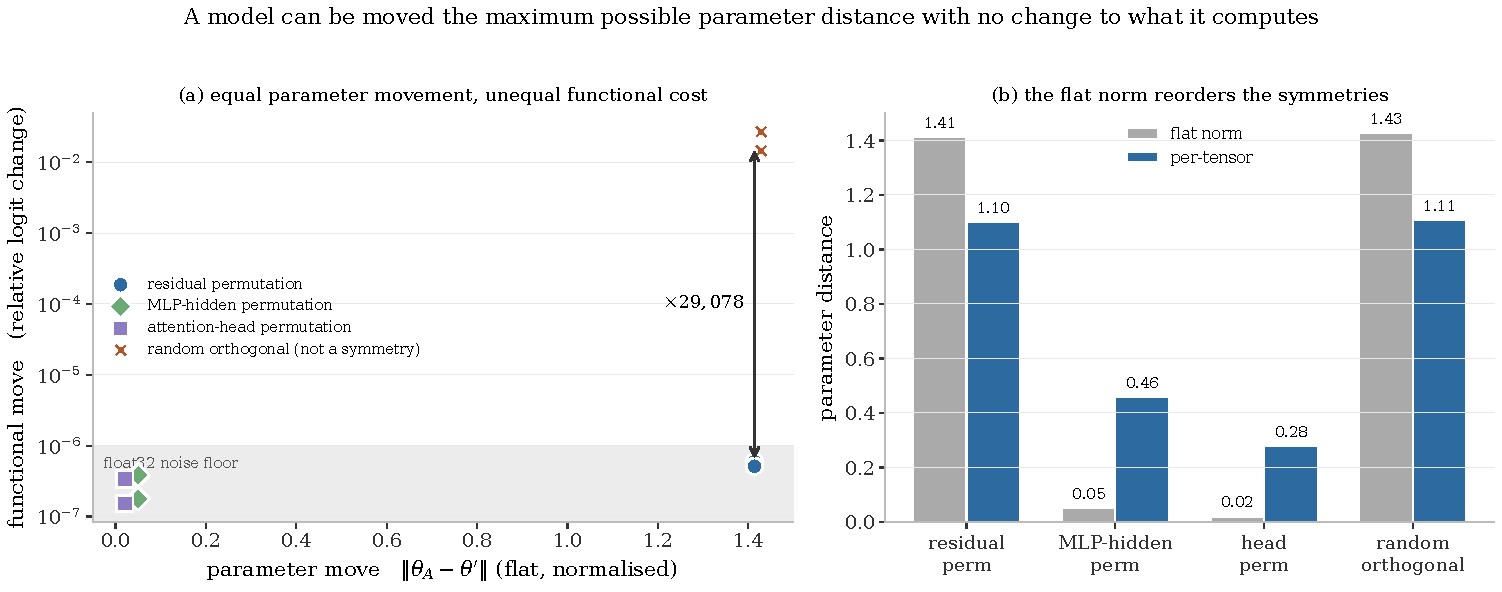
\includegraphics[width=\textwidth,height=0.74\textheight,keepaspectratio]{figures/fig23_invariance.pdf}
  \end{center}
  \vspace{-0.5em}\begin{center}\tiny A valid permutation moves the weights maximally and preserves the function; a random orthogonal moves them as far and breaks it \par {\tiny\texttt{\detokenize{fig23_invariance.pdf}}}\end{center}
\end{frame}

\begin{frame}{The provenance ladder}
  \begin{center}
    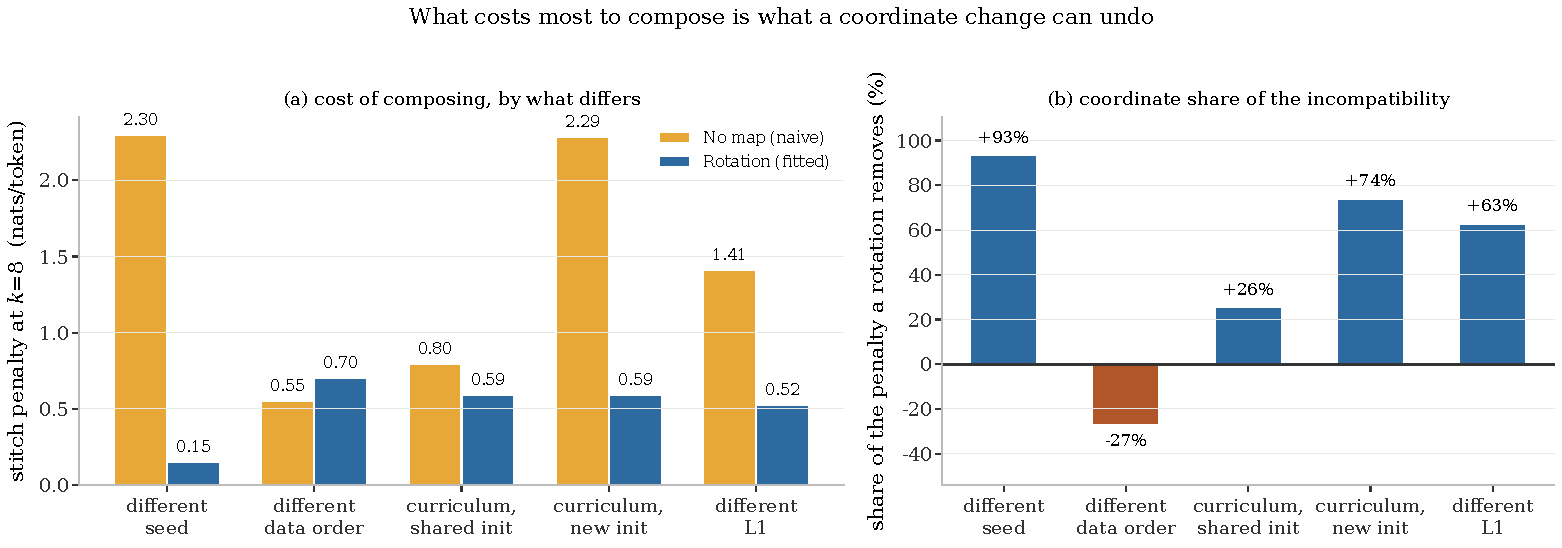
\includegraphics[width=\textwidth,height=0.74\textheight,keepaspectratio]{figures/fig21_provenance_ladder.pdf}
  \end{center}
  \vspace{-0.5em}\begin{center}\tiny Cost of composing at a mid-depth seam, and the share a fitted map removes \par {\tiny\texttt{\detokenize{fig21_provenance_ladder.pdf}}}\end{center}
\end{frame}

\begin{frame}{Stitch curves}
  \begin{center}
    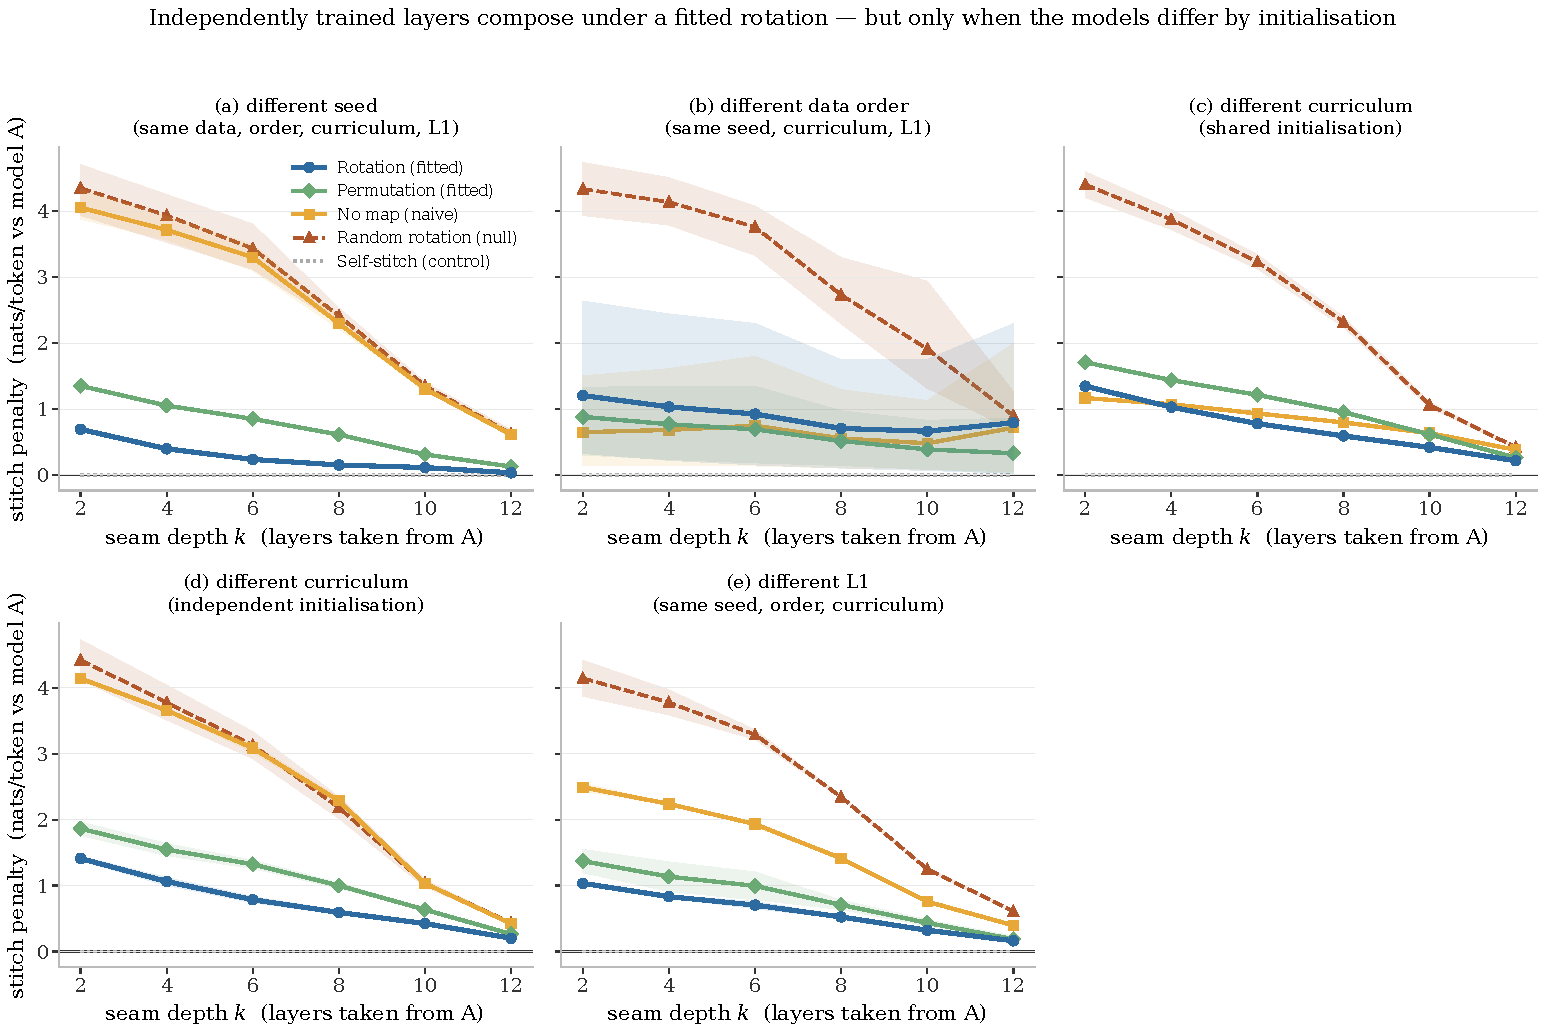
\includegraphics[width=\textwidth,height=0.74\textheight,keepaspectratio]{figures/fig20_stitch_curves.pdf}
  \end{center}
  \vspace{-0.5em}\begin{center}\tiny Penalty as a function of the seam depth \par {\tiny\texttt{\detokenize{fig20_stitch_curves.pdf}}}\end{center}
\end{frame}

\begin{frame}{The diagnostic}
  \begin{center}
    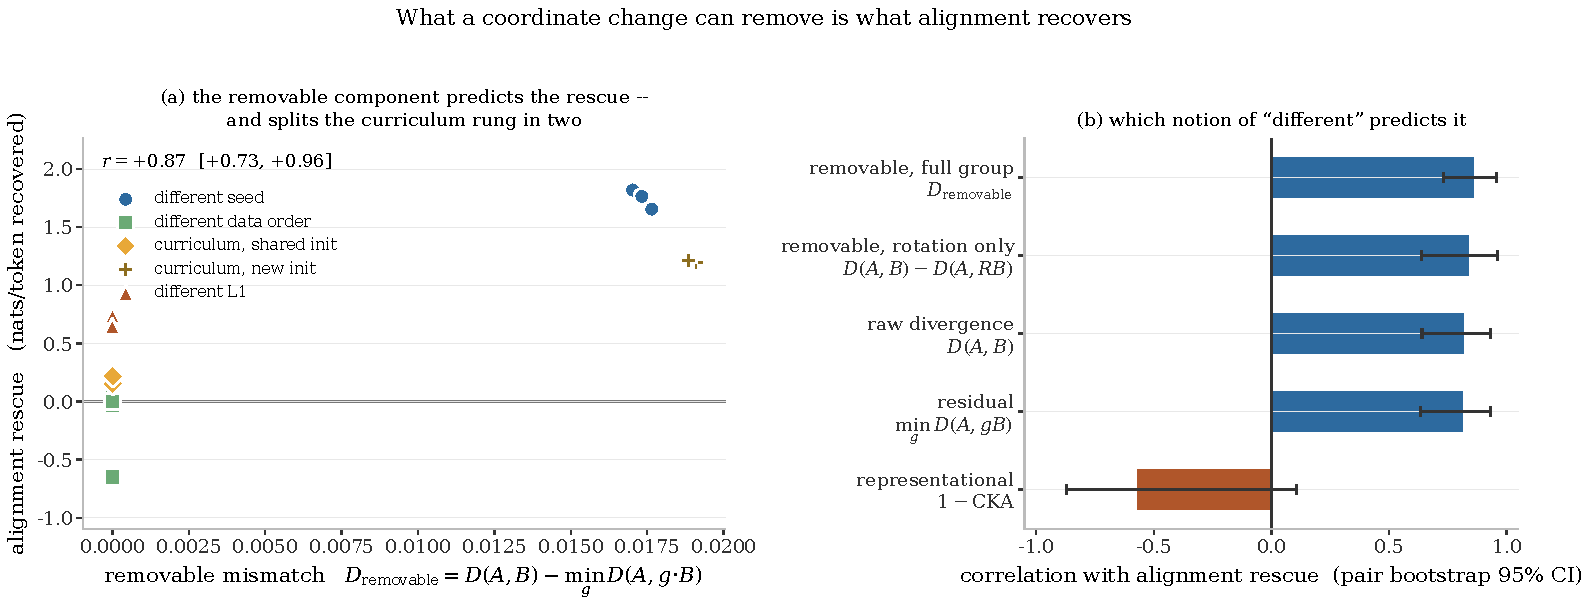
\includegraphics[width=\textwidth,height=0.74\textheight,keepaspectratio]{figures/fig22_signature.pdf}
  \end{center}
  \vspace{-0.5em}\begin{center}\tiny Removable component against the rescue alignment delivers, one point per pair \par {\tiny\texttt{\detokenize{fig22_signature.pdf}}}\end{center}
\end{frame}

\begin{frame}{2,320 merges, cut on initialisation}
  \begin{center}
    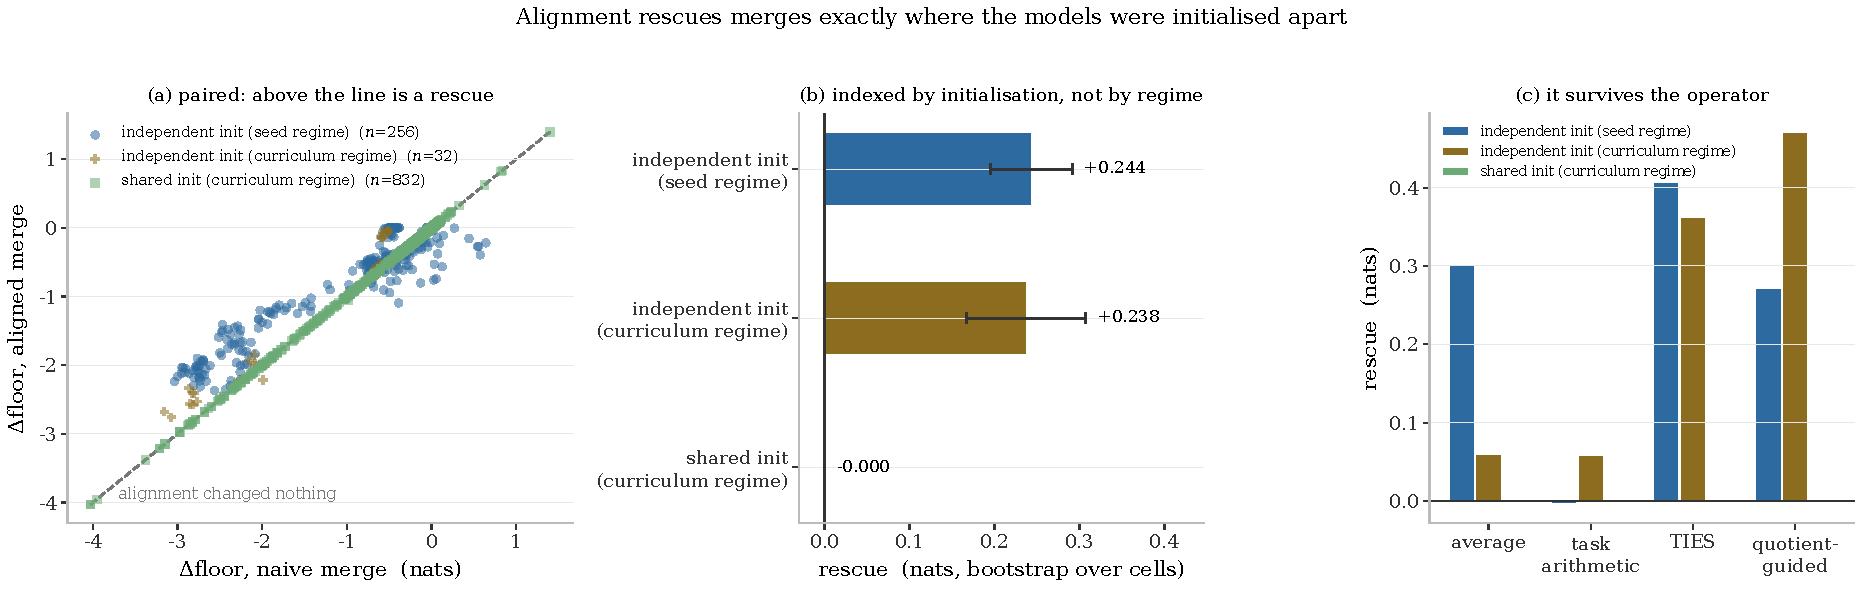
\includegraphics[width=\textwidth,height=0.74\textheight,keepaspectratio]{figures/fig26_merge_rescue.pdf}
  \end{center}
  \vspace{-0.5em}\begin{center}\tiny Paired naive vs aligned per cell; effect size by class; operator invariance \par {\tiny\texttt{\detokenize{fig26_merge_rescue.pdf}}}\end{center}
\end{frame}

\begin{frame}{The distance-matched control}
  \begin{center}
    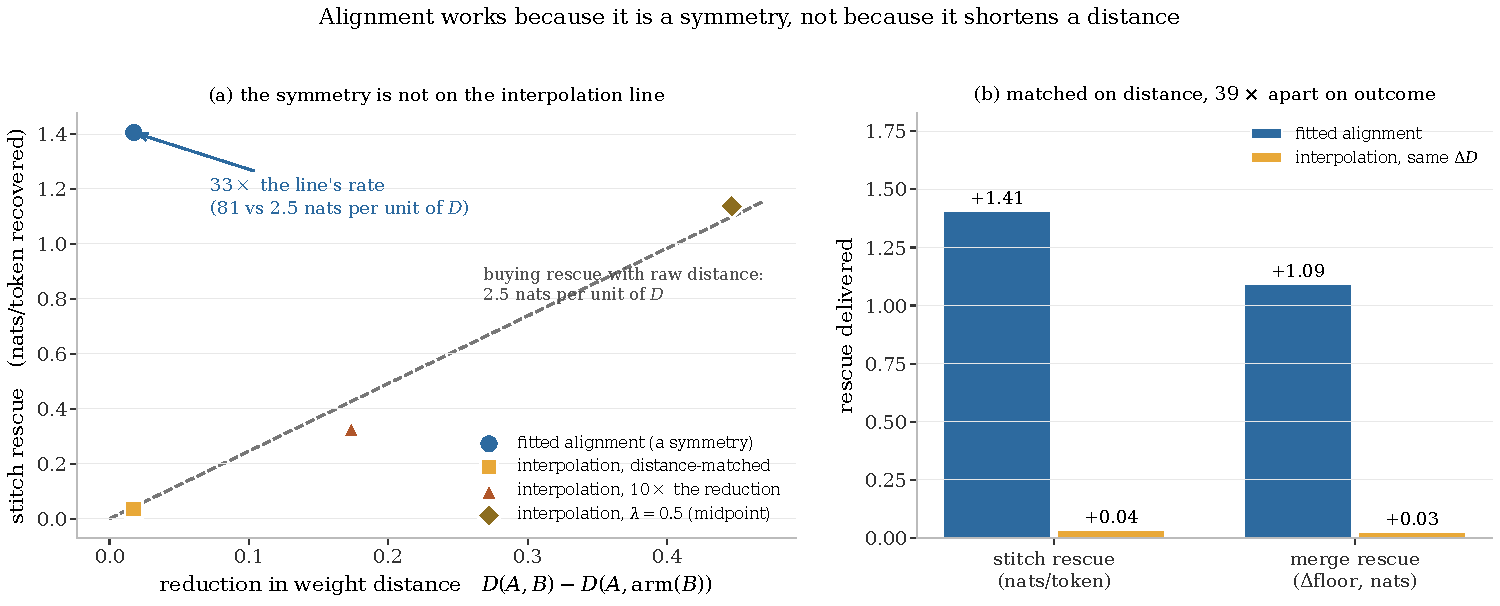
\includegraphics[width=\textwidth,height=0.74\textheight,keepaspectratio]{figures/fig25_distance_matched.pdf}
  \end{center}
  \vspace{-0.5em}\begin{center}\tiny Rescue against the reduction in weight distance that bought it \par {\tiny\texttt{\detokenize{fig25_distance_matched.pdf}}}\end{center}
\end{frame}

\begin{frame}{The symmetry-class bake-off}
  \begin{center}
    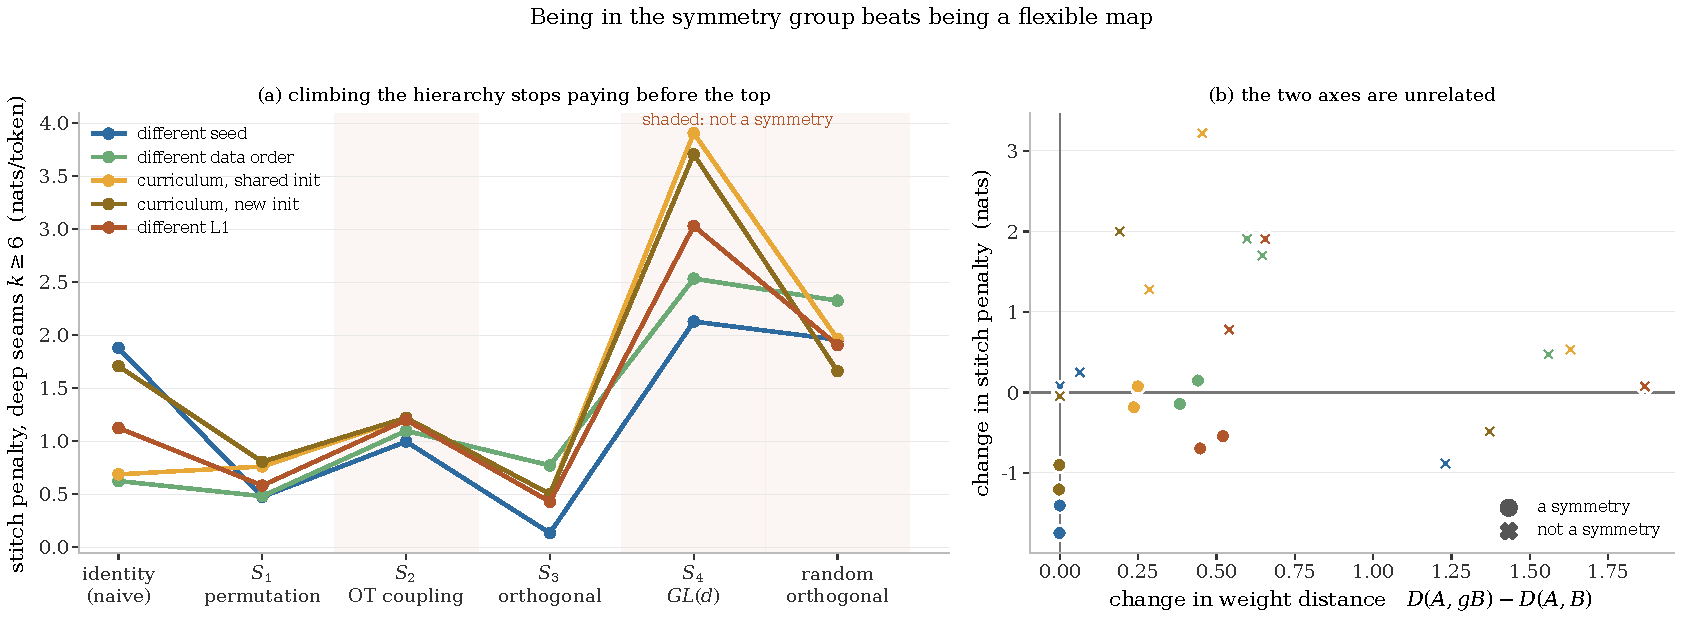
\includegraphics[width=\textwidth,height=0.74\textheight,keepaspectratio]{figures/fig27_group_ladder.pdf}
  \end{center}
  \vspace{-0.5em}\begin{center}\tiny Benefit peaks at the orthogonal class and collapses at GL(d) \par {\tiny\texttt{\detokenize{fig27_group_ladder.pdf}}}\end{center}
\end{frame}

\begin{frame}{The training trajectory}
  \begin{center}
    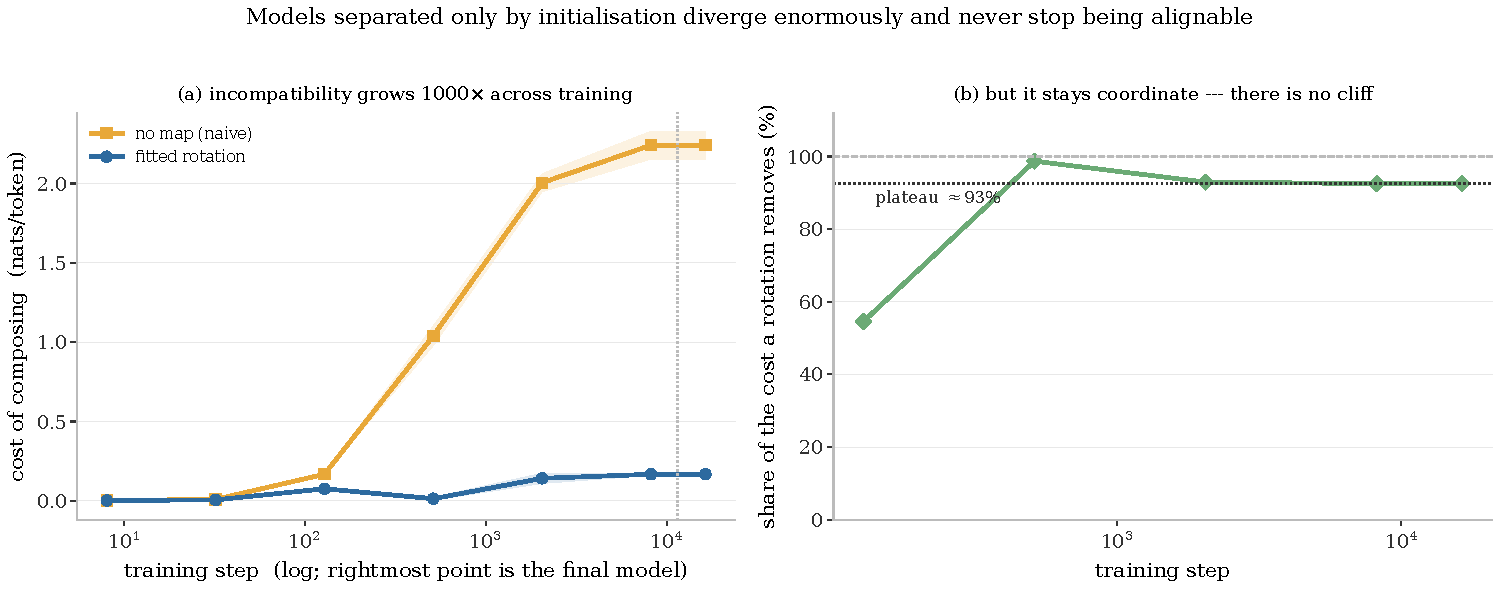
\includegraphics[width=\textwidth,height=0.74\textheight,keepaspectratio]{figures/fig24_trajectory.pdf}
  \end{center}
  \vspace{-0.5em}\begin{center}\tiny Cost of composing grows 916x while the removable share stays above 92\% \par {\tiny\texttt{\detokenize{fig24_trajectory.pdf}}}\end{center}
\end{frame}

\begin{frame}{External replication: PolyPythia}
  \begin{center}
    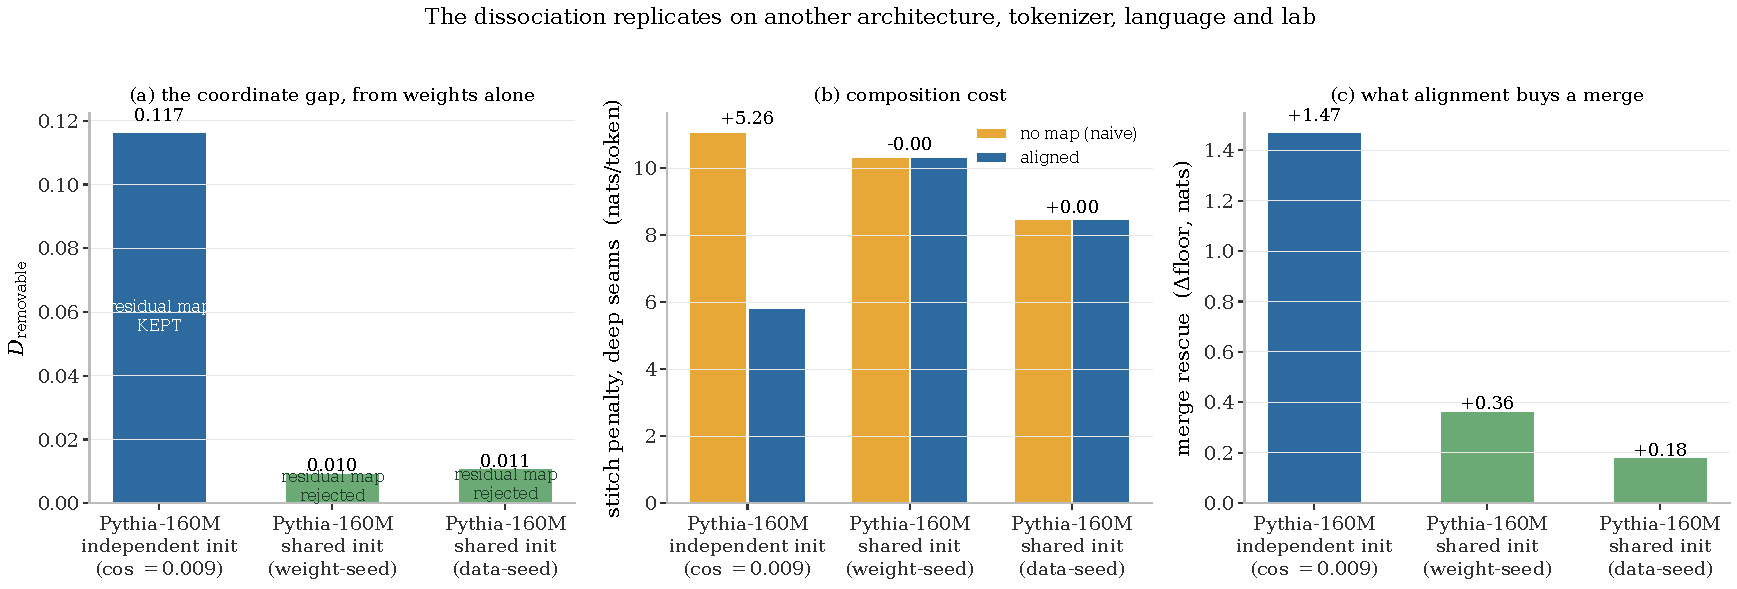
\includegraphics[width=\textwidth,height=0.74\textheight,keepaspectratio]{figures/fig28_external.pdf}
  \end{center}
  \vspace{-0.5em}\begin{center}\tiny A different architecture, tokenizer, language, corpus and lab \par {\tiny\texttt{\detokenize{fig28_external.pdf}}}\end{center}
\end{frame}

\section{Tables}

\begin{frame}{Table 1}
  \centering
  \scriptsize
  \small
\begin{tabular}{lrrr}
\toprule
transformation & $D$ & flat $\lVert\cdot\rVert$ & logit change \\
\midrule
residual permutation      & $1.1006$ & $1.4139$ & $5.8\times10^{-7}$ \\
MLP-hidden permutation    & $0.4598$ & $0.0501$ & $3.4\times10^{-7}$ \\
head permutation          & $0.2808$ & $0.0206$ & $3.0\times10^{-7}$ \\
\textbf{random orthogonal}& $1.1070$ & $1.4287$ & $\mathbf{1.7\times10^{-2}}$ \\
\bottomrule
\end{tabular}
  \vspace{0.6em}
  \begin{center}\tiny Mean over five checkpoints. Only the last is not a symmetry.\end{center}
\end{frame}

\begin{frame}{Table 2}
  \centering
  \scriptsize
  \small
\begin{tabular}{lrrrr}
\toprule
what differs & $n$ & naive & aligned & coord.\ share \\
\midrule
\textbf{initialisation}       & 3 & $2.298$ & $\mathbf{0.150}$ & $\mathbf{+93\%}$ \\
data order                    & 4 & $0.553$ & $0.705$ & $-27\%$ \\
curriculum, shared init       & 2 & $0.796$ & $0.592$ & $+26\%$ \\
curriculum, new init          & 2 & $2.287$ & $0.593$ & $\mathbf{+74\%}$ \\
first language                & 2 & $1.412$ & $0.524$ & $+63\%$ \\
\bottomrule
\end{tabular}
  \vspace{0.6em}
  \begin{center}\tiny Stitch penalty (nats/token) at seam $k{=}8$ of $14$. The self-stitch control $B{:=}A$ is
exactly $0.000$ at every seam and rung; a random orthogonal is worse than no map everywhere, by
factors of two to five.\end{center}
\end{frame}

\begin{frame}{Table 3}
  \centering
  \scriptsize
  \small
\begin{tabular}{lrrrr}
\toprule
& pairs & rescue & 95\% CI & improved \\
\midrule
indep.\ init (seed regime)  & 64  & $+0.244$ & $[+0.163,+0.321]$ & $73\%$ \\
indep.\ init (curric.\ reg.)& 8   & $+0.238$ & $[+0.214,+0.261]$ & $94\%$ \\
\textbf{shared init}        & 208 & $-0.000$ & $[-0.000,+0.000]$ & $7\%$ \\
\bottomrule
\end{tabular}
  \vspace{0.6em}
  \begin{center}\tiny Cut on initialisation, not on the experiment's own regime labels.\end{center}
\end{frame}

\begin{frame}{Table 4}
  \centering
  \scriptsize
  \small
\begin{tabular}{lrrrrr}
\toprule
what differs & id. & $S_1$ & $S_2$ & $S_3$ & $S_4$ \\
\midrule
initialisation        & $1.880$ & $0.474$ & $0.995$ & $\mathbf{0.132}$ & $2.128$ \\
data order            & $0.624$ & $\mathbf{0.480}$ & $1.097$ & $0.770$ & $2.534$ \\
curric., shared init  & $0.686$ & $0.761$ & $1.217$ & $\mathbf{0.501}$ & $3.906$ \\
curric., new init     & $1.707$ & $0.805$ & $1.220$ & $\mathbf{0.500}$ & $3.707$ \\
first language        & $1.124$ & $0.581$ & $1.199$ & $\mathbf{0.428}$ & $3.030$ \\
\bottomrule
\end{tabular}
  \vspace{0.6em}
  \begin{center}\tiny Stitch penalty, deep seams. A random orthogonal scores $1.66$--$2.33$ across these rungs.\end{center}
\end{frame}

\begin{frame}{Table 5}
  \centering
  \scriptsize
  \small
\begin{tabular}{lcc}
\toprule
checkpoint & shared init & independent init \\
\midrule
\texttt{step-0}    & $1.0000$ & $0.0003$ \\
\texttt{step-2}    & $1.0000$ & $0.0003$ \\
\texttt{step-16}   & $1.0000$ & $0.0003$ \\
\texttt{step-128}  & $1.0000$ & $0.0003$ \\
\texttt{step-1024} & $1.0000$ & $0.0003$ \\
\texttt{step-2048} & $1.0000$ & $0.0003$ \\
\texttt{main}      & $\mathbf{1.0000}$ & $\mathbf{0.0003}$ \\
\bottomrule
\end{tabular}
  \vspace{0.6em}
  \begin{center}\tiny Identity-match fraction on the per-layer MLP hidden axis, mean over pairs. Chance is
$1/768 = 0.0013$. The shared-init column is $1.0000$ at every checkpoint and its minimum over
\emph{every layer of every checkpoint} is also $1.0000$: not one unit out of $3072 \times 14$ ever
swaps. The residual basis gives the same answer ($1.0000$ against $0.0007$).\end{center}
\end{frame}

\begin{frame}{Table 6}
  \centering
  \scriptsize
  \small
\begin{tabular}{lrrrr}
\toprule
Pythia-160M & cos & $\Drem$ & stitch & merge \\
\midrule
indep.\ init (\texttt{seed})   & $0.009$ & $\mathbf{0.117}$ & $11.08{\to}5.82$ & $\mathbf{+1.47}$ \\
shared (\texttt{weight-seed})  & $0.538$ & $0.010$ & $10.33{\to}10.33$ & $+0.37$ \\
shared (\texttt{data-seed})    & $0.549$ & $0.011$ & $8.49{\to}8.49$ & $+0.18$ \\
\bottomrule
\end{tabular}
  \vspace{0.6em}
  \begin{center}\tiny The residual-basis factor survives acceptance on exactly the independently initialised pairs.\end{center}
\end{frame}

\begin{frame}{Table 7}
  \centering
  \scriptsize
  \small
\begin{tabular}{lrrrr}
\toprule
predictor & AUROC & AUPRC & prec. & rec. \\
\midrule
$\mathrm{QMD}_{\text{per-tensor}}$ & $\mathbf{0.944}$ & $\mathbf{0.796}$ & $0.727$ & $0.760$ \\
weight cosine                      & $0.933$ & $0.712$ & $0.557$ & $0.881$ \\
$\Drem$ share                      & $0.926$ & $0.699$ & $0.679$ & $0.882$ \\
naive merge barrier                & $0.919$ & $0.789$ & $0.589$ & $0.811$ \\
search verdict (binary)            & $0.802$ & $0.589$ & $0.351$ & $0.928$ \\
CKA                                & $0.319$ & $0.177$ & $0.252$ & $0.997$ \\
\bottomrule
\end{tabular}
  \vspace{0.6em}
  \begin{center}\tiny Held-out prediction of ``will aligning this pair improve $\Delta$floor'', $1{,}120$ cells /
$280$ pairs, base rate $0.250$, split on pairs over $200$ repetitions.\end{center}
\end{frame}

\begin{frame}{Table 8}
  \centering
  \scriptsize
  \small
\begin{tabular}{lrrrr}
\toprule
$k$ & 2 & 3 & 4 & 5 \\
\midrule
naive $\Delta$floor   & $-1.864$ & $-3.276$ & $-3.739$ & $-3.950$ \\
aligned $\Delta$floor & $-0.992$ & $-1.325$ & $-1.376$ & $\mathbf{-1.494}$ \\
rescue                & $+0.871$ & $+1.951$ & $+2.363$ & $\mathbf{+2.455}$ \\
\bottomrule
\end{tabular}
  \vspace{0.6em}
  \begin{center}\tiny $k$-way merging of independently initialised models, unweighted average, all carried into
model 1's frame.\end{center}
\end{frame}

\begin{frame}{Table 9}
  \centering
  \scriptsize
  \small
\begin{tabular}{llrrr}
\toprule
what differs & language & $n$ & naive & coordinate share \\
\midrule
independent init & \texttt{nld-eng} & 16 & $2.236$ & $+92\%$ $[+91, +93]$ \\
independent init & \texttt{deu-eng} & 6  & $2.324$ & $+89\%$ $[+81, +94]$ \\
independent init & \texttt{zho-eng} & 6  & $2.122$ & $+93\%$ $[+91, +95]$ \\
data order (shared init) & \texttt{nld-eng} & 8 & $0.567$ & $-26\%$ $[-50, +2]$ \\
\bottomrule
\end{tabular}
  \vspace{0.6em}
  \begin{center}\tiny The provenance ladder across three language pairs, pair-level bootstrap intervals.\end{center}
\end{frame}

\begin{frame}{Table 10}
  \centering
  \scriptsize
  \small
\begin{tabular}{lrrrr}
\toprule
& $n$ & $\Drem$ & residual factor kept & merge rescue \\
\midrule
Pythia-14M  & 36 & $0.122$ & $36/36$ & $+23.6$ $[+21.5, +25.8]$ \\
Pythia-70M  & 36 & $0.097$ & $36/36$ & $+6.1$ $[+4.4, +7.6]$ \\
Pythia-160M & 2  & $0.117$ & $2/2$   & $+1.5$ \\
\bottomrule
\end{tabular}
  \vspace{0.6em}
  \begin{center}\tiny External replication across three scales, all $\binom{9}{2}$ reseeded pairs at 14M and 70M.\end{center}
\end{frame}

\begin{frame}{Table 11}
  \centering
  \scriptsize
  \begin{tabular}{lrrr}
\toprule
arm & $\Delta D$ & stitch rescue & per unit $\Delta D$ \\
\midrule
fitted alignment       & $0.0173$ & $\mathbf{+1.405}$ & $\mathbf{81.1}$ \\
interpolation, matched & $0.0173$ & $+0.036$ & $2.1$ \\
interpolation, $10\times$ & $0.1733$ & $+0.327$ & $1.9$ \\
interpolation, $\lambda{=}0.5$ & $0.4466$ & $+1.138$ & $2.5$ \\
\bottomrule
\end{tabular}
\end{frame}

\section{Representational analysis (jrf\_beetle)}

\subsection{Layer-wise CKA}

\begin{frame}{fig01: Layerwise CKA eng nld main combined}
  \begin{center}
    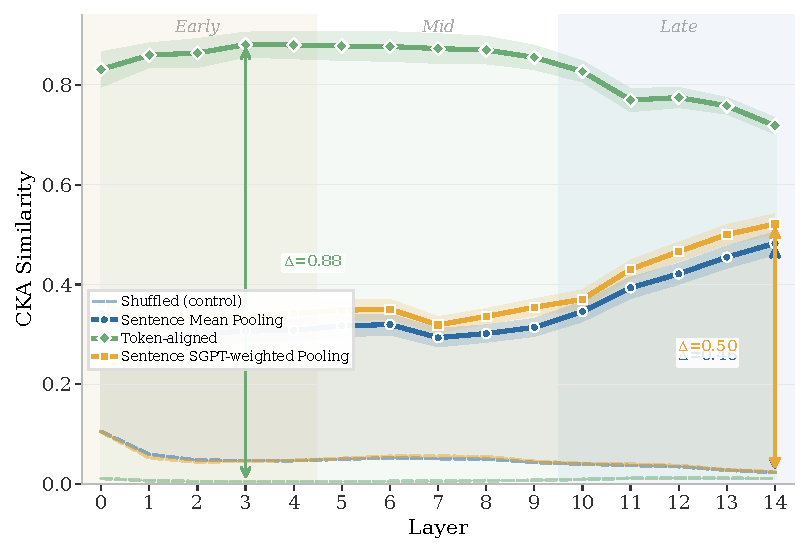
\includegraphics[width=\textwidth,height=0.74\textheight,keepaspectratio]{figures/fig01_layerwise_cka_eng_nld_main_combined.pdf}
  \end{center}
  \vspace{-0.5em}\begin{center}\tiny {\tiny\texttt{\detokenize{fig01_layerwise_cka_eng_nld_main_combined.pdf}}}\end{center}
\end{frame}

\begin{frame}{fig01: Layerwise CKA eng nld main panels}
  \begin{center}
    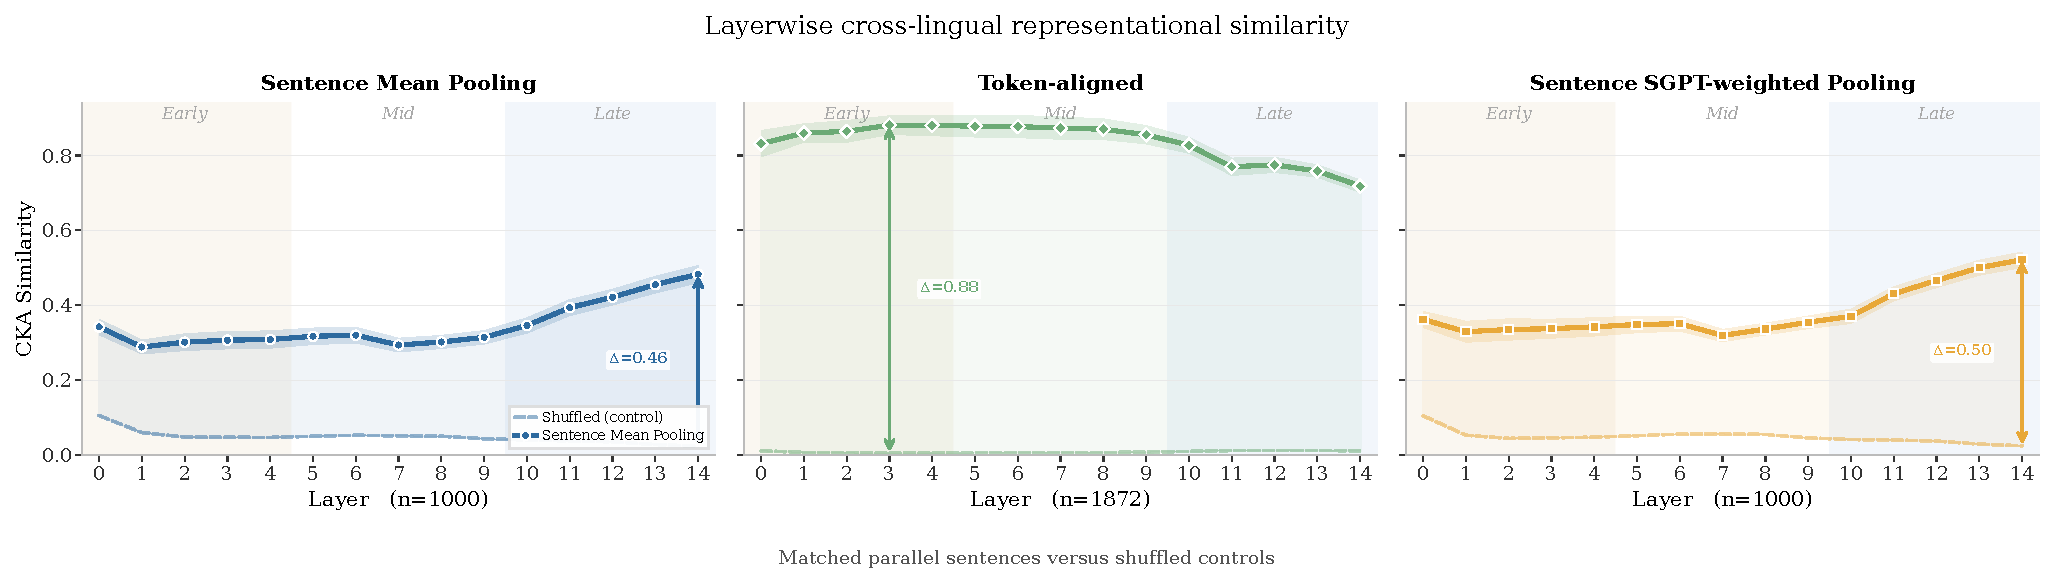
\includegraphics[width=\textwidth,height=0.74\textheight,keepaspectratio]{figures/fig01_layerwise_cka_eng_nld_main_panels.pdf}
  \end{center}
  \vspace{-0.5em}\begin{center}\tiny {\tiny\texttt{\detokenize{fig01_layerwise_cka_eng_nld_main_panels.pdf}}}\end{center}
\end{frame}

\begin{frame}{fig01: Layerwise CKA bilingual}
  \begin{center}
    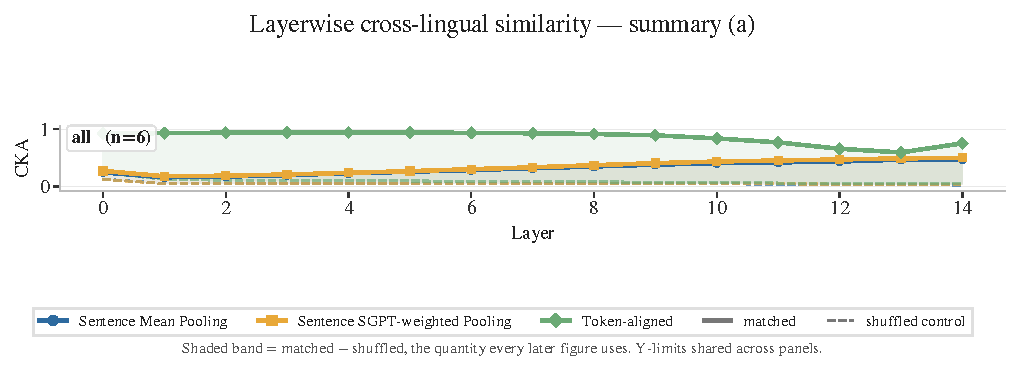
\includegraphics[width=\textwidth,height=0.74\textheight,keepaspectratio]{figures/fig01a_layerwise_cka_bilingual.pdf}
  \end{center}
  \vspace{-0.5em}\begin{center}\tiny {\tiny\texttt{\detokenize{fig01a_layerwise_cka_bilingual.pdf}}}\end{center}
\end{frame}

\begin{frame}{fig01: Layerwise CKA families}
  \begin{center}
    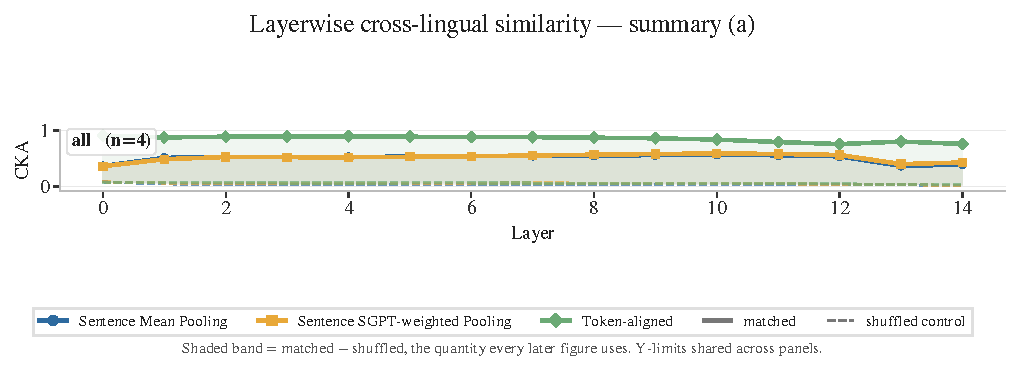
\includegraphics[width=\textwidth,height=0.74\textheight,keepaspectratio]{figures/fig01a_layerwise_cka_families.pdf}
  \end{center}
  \vspace{-0.5em}\begin{center}\tiny {\tiny\texttt{\detokenize{fig01a_layerwise_cka_families.pdf}}}\end{center}
\end{frame}

\begin{frame}{fig01: Layerwise CKA mono}
  \begin{center}
    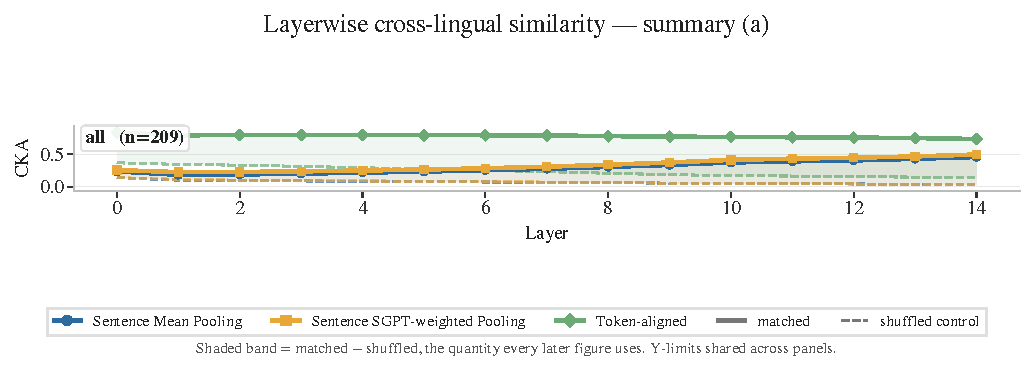
\includegraphics[width=\textwidth,height=0.74\textheight,keepaspectratio]{figures/fig01a_layerwise_cka_mono.pdf}
  \end{center}
  \vspace{-0.5em}\begin{center}\tiny {\tiny\texttt{\detokenize{fig01a_layerwise_cka_mono.pdf}}}\end{center}
\end{frame}

\begin{frame}{fig01: Layerwise CKA bilingual}
  \begin{center}
    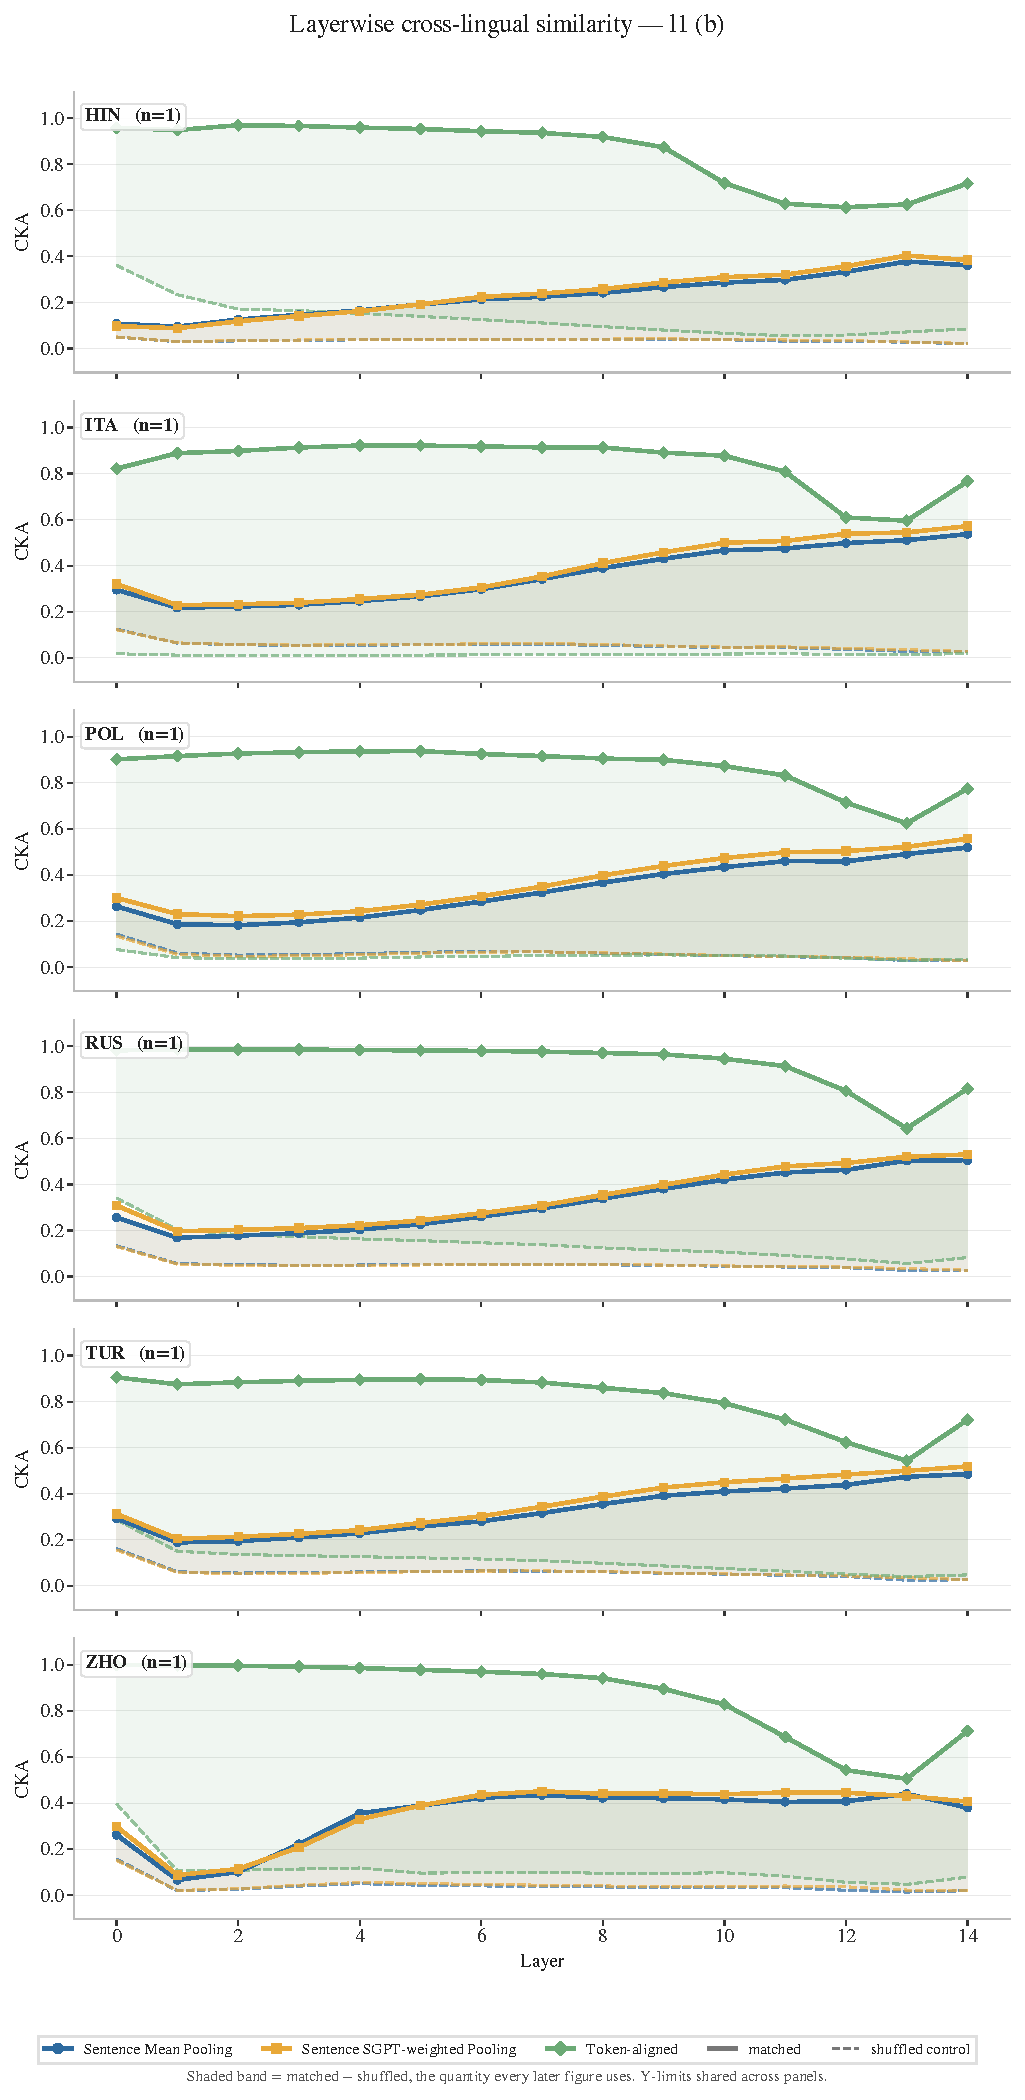
\includegraphics[width=\textwidth,height=0.74\textheight,keepaspectratio]{figures/fig01b_layerwise_cka_bilingual.pdf}
  \end{center}
  \vspace{-0.5em}\begin{center}\tiny {\tiny\texttt{\detokenize{fig01b_layerwise_cka_bilingual.pdf}}}\end{center}
\end{frame}

\begin{frame}{fig01: Layerwise CKA families}
  \begin{center}
    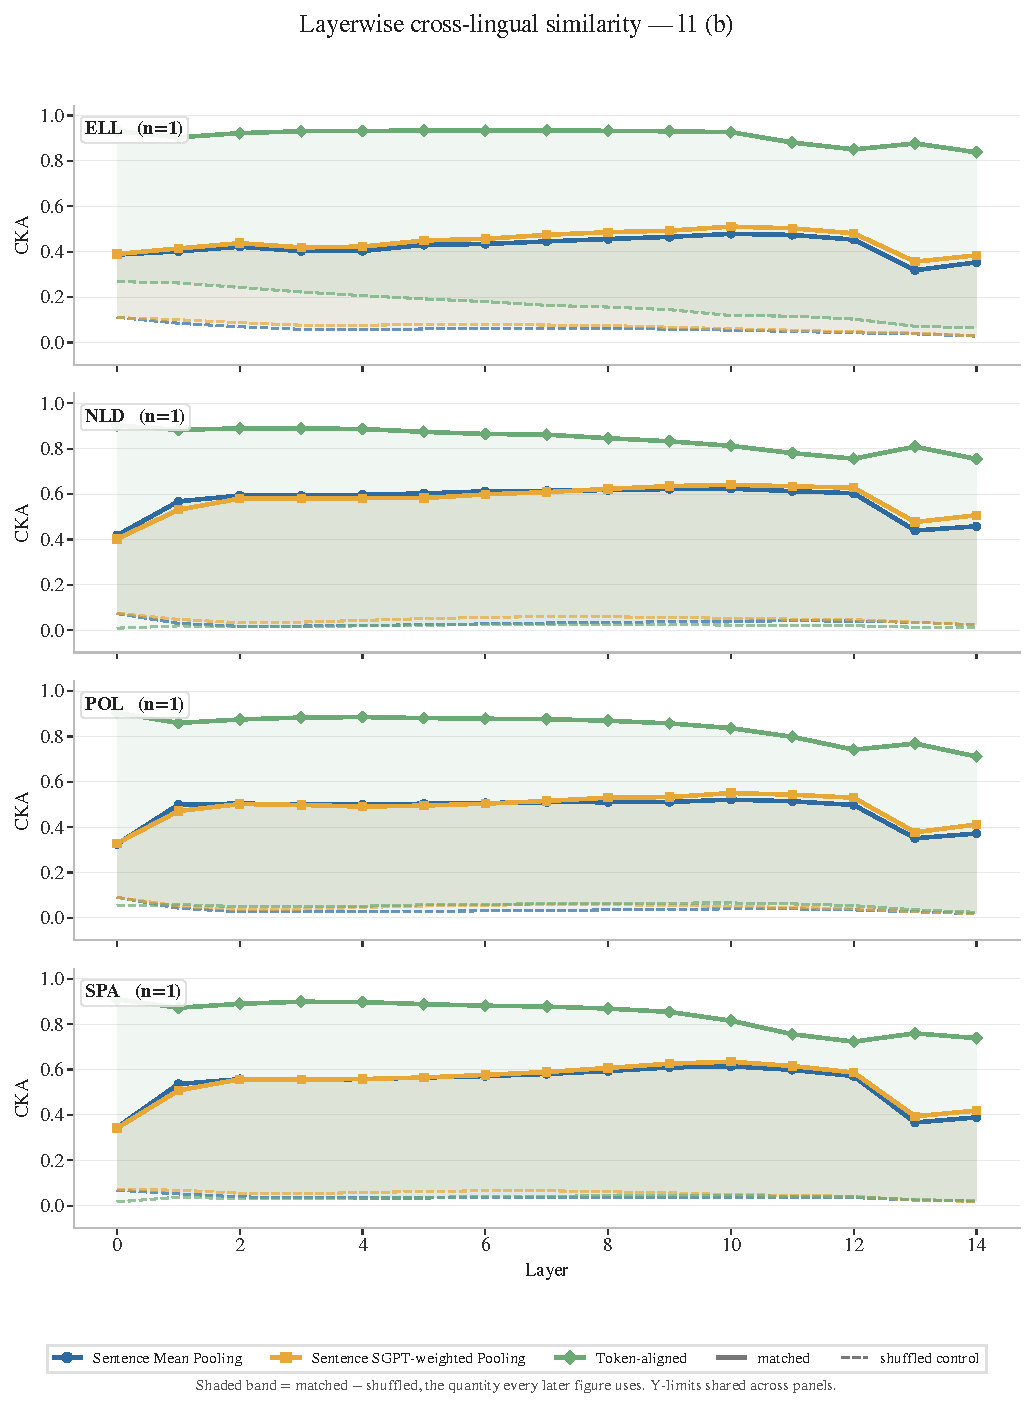
\includegraphics[width=\textwidth,height=0.74\textheight,keepaspectratio]{figures/fig01b_layerwise_cka_families.pdf}
  \end{center}
  \vspace{-0.5em}\begin{center}\tiny {\tiny\texttt{\detokenize{fig01b_layerwise_cka_families.pdf}}}\end{center}
\end{frame}

\begin{frame}{fig01: Layerwise CKA mono}
  \begin{center}
    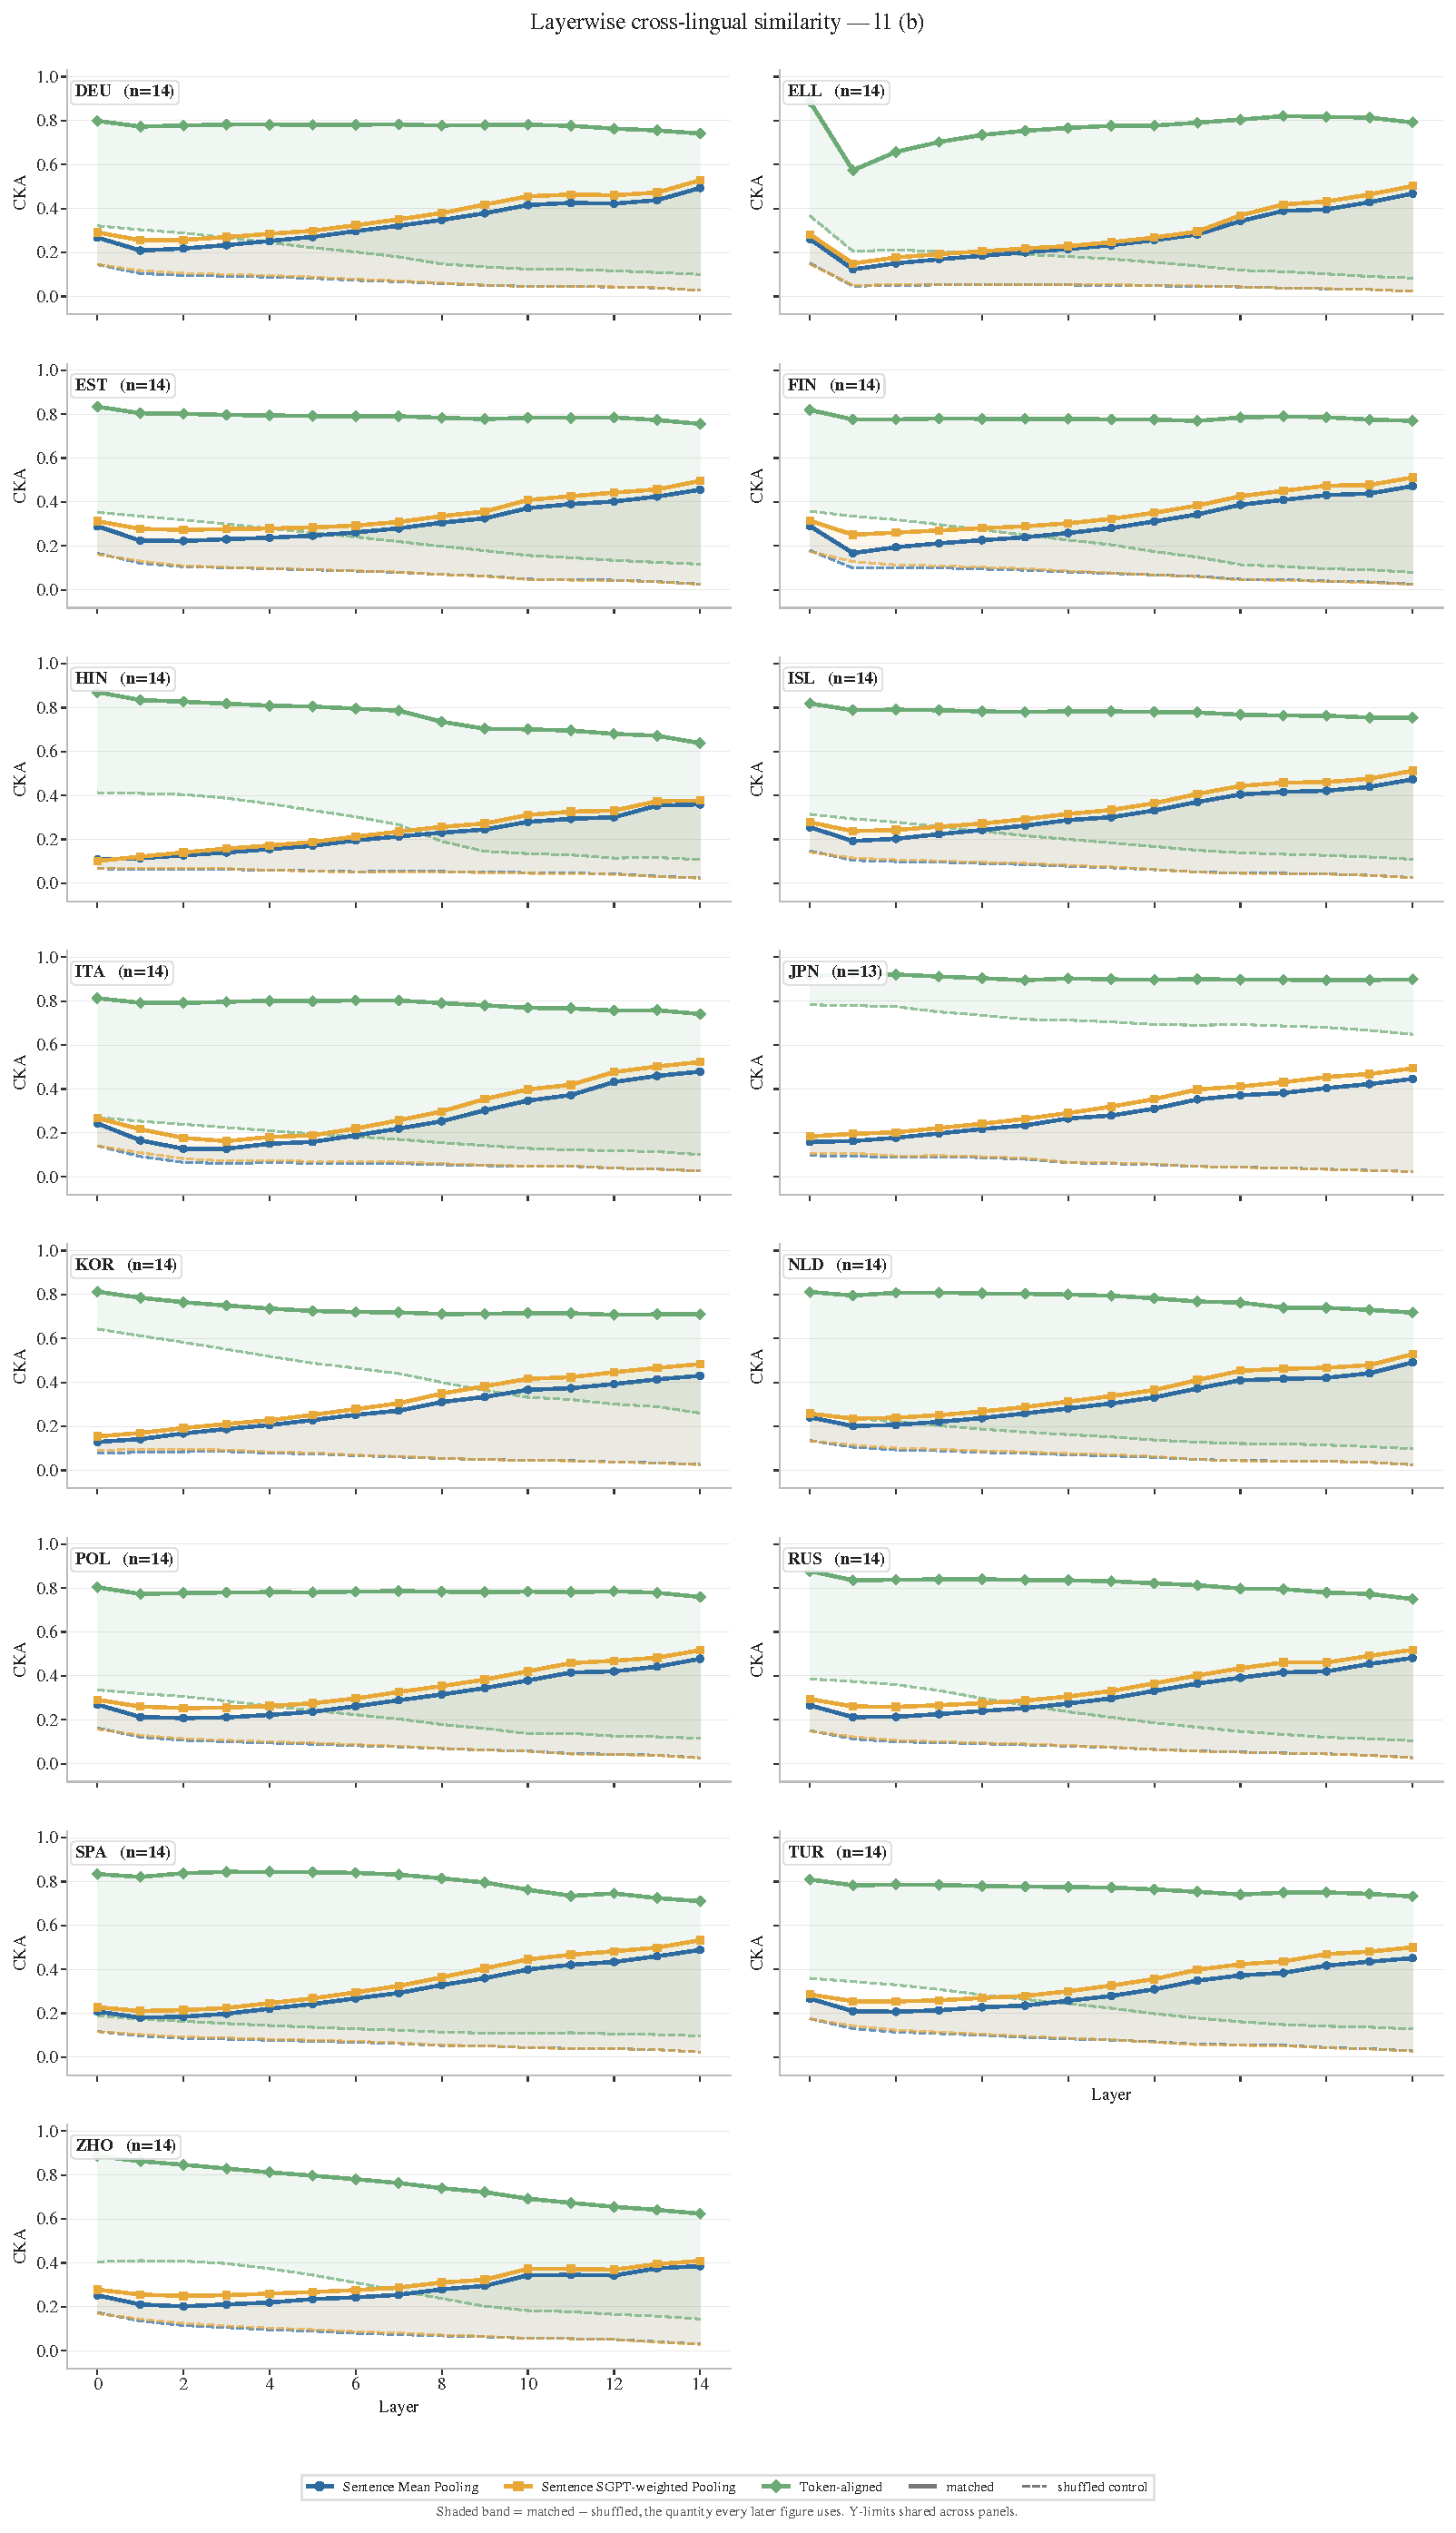
\includegraphics[width=\textwidth,height=0.74\textheight,keepaspectratio]{figures/fig01b_layerwise_cka_mono.pdf}
  \end{center}
  \vspace{-0.5em}\begin{center}\tiny {\tiny\texttt{\detokenize{fig01b_layerwise_cka_mono.pdf}}}\end{center}
\end{frame}

\begin{frame}{fig01: Layerwise CKA bilingual}
  \begin{center}
    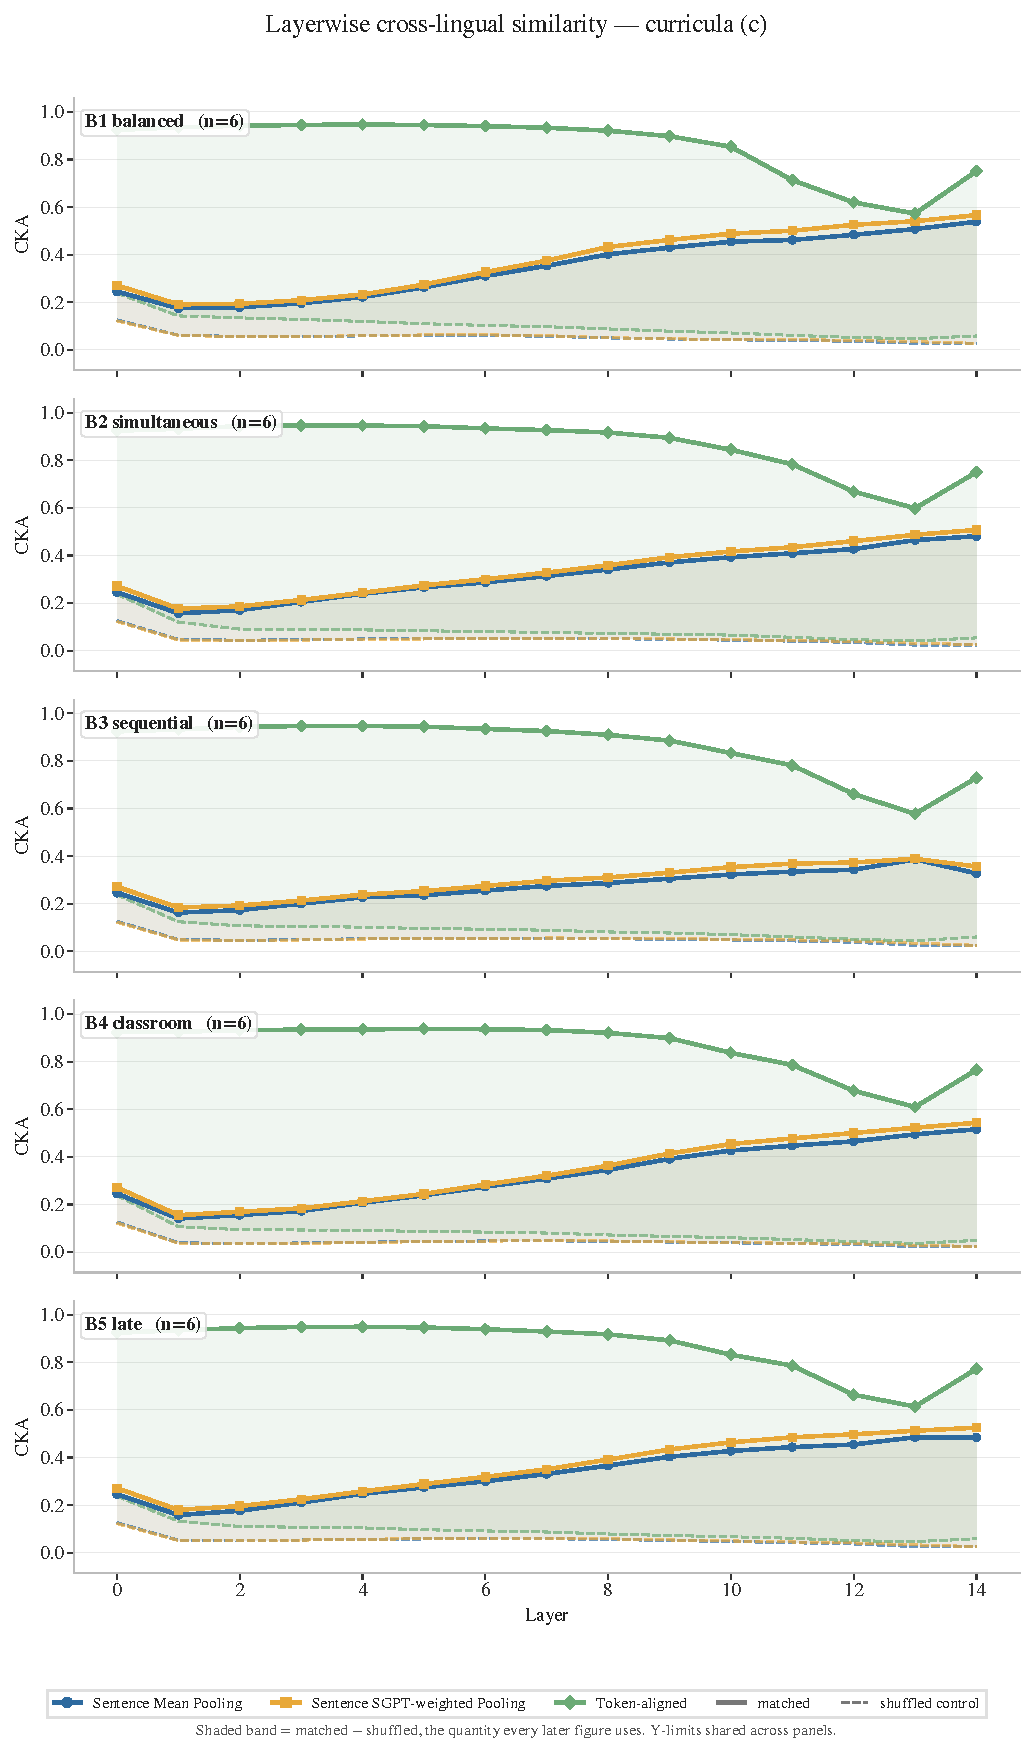
\includegraphics[width=\textwidth,height=0.74\textheight,keepaspectratio]{figures/fig01c_layerwise_cka_bilingual.pdf}
  \end{center}
  \vspace{-0.5em}\begin{center}\tiny {\tiny\texttt{\detokenize{fig01c_layerwise_cka_bilingual.pdf}}}\end{center}
\end{frame}

\begin{frame}{fig01: Layerwise CKA families}
  \begin{center}
    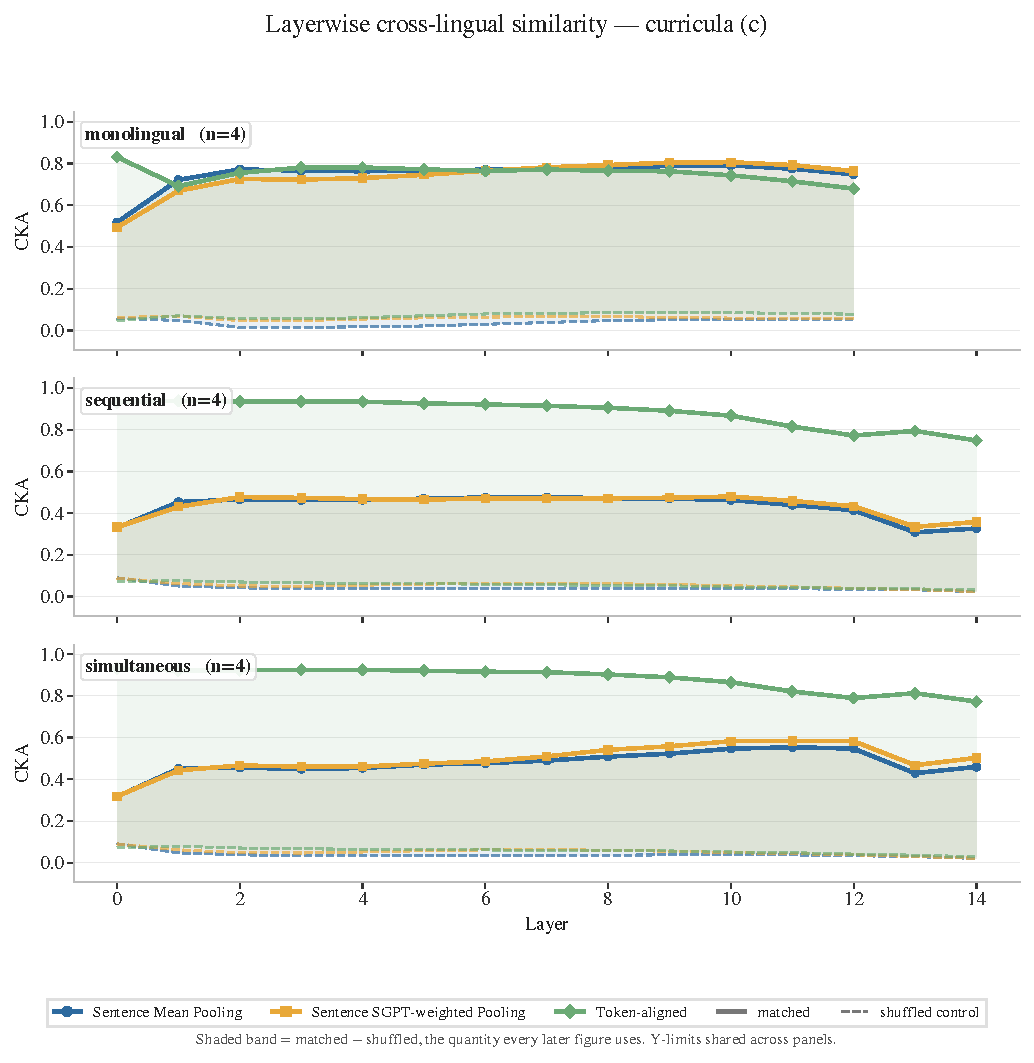
\includegraphics[width=\textwidth,height=0.74\textheight,keepaspectratio]{figures/fig01c_layerwise_cka_families.pdf}
  \end{center}
  \vspace{-0.5em}\begin{center}\tiny {\tiny\texttt{\detokenize{fig01c_layerwise_cka_families.pdf}}}\end{center}
\end{frame}

\begin{frame}{fig01: Layerwise CKA bilingual}
  \begin{center}
    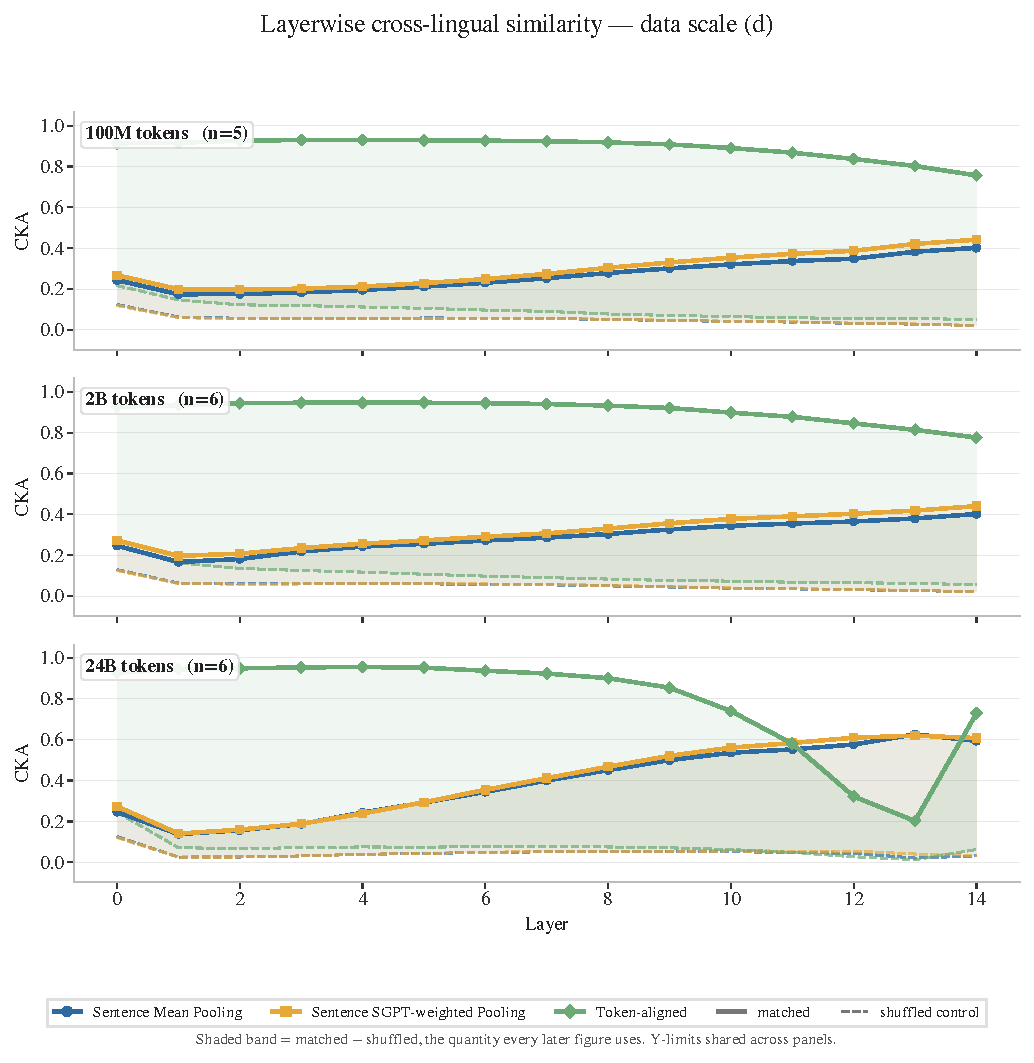
\includegraphics[width=\textwidth,height=0.74\textheight,keepaspectratio]{figures/fig01d_layerwise_cka_bilingual.pdf}
  \end{center}
  \vspace{-0.5em}\begin{center}\tiny {\tiny\texttt{\detokenize{fig01d_layerwise_cka_bilingual.pdf}}}\end{center}
\end{frame}

\begin{frame}{fig01: Layerwise CKA families}
  \begin{center}
    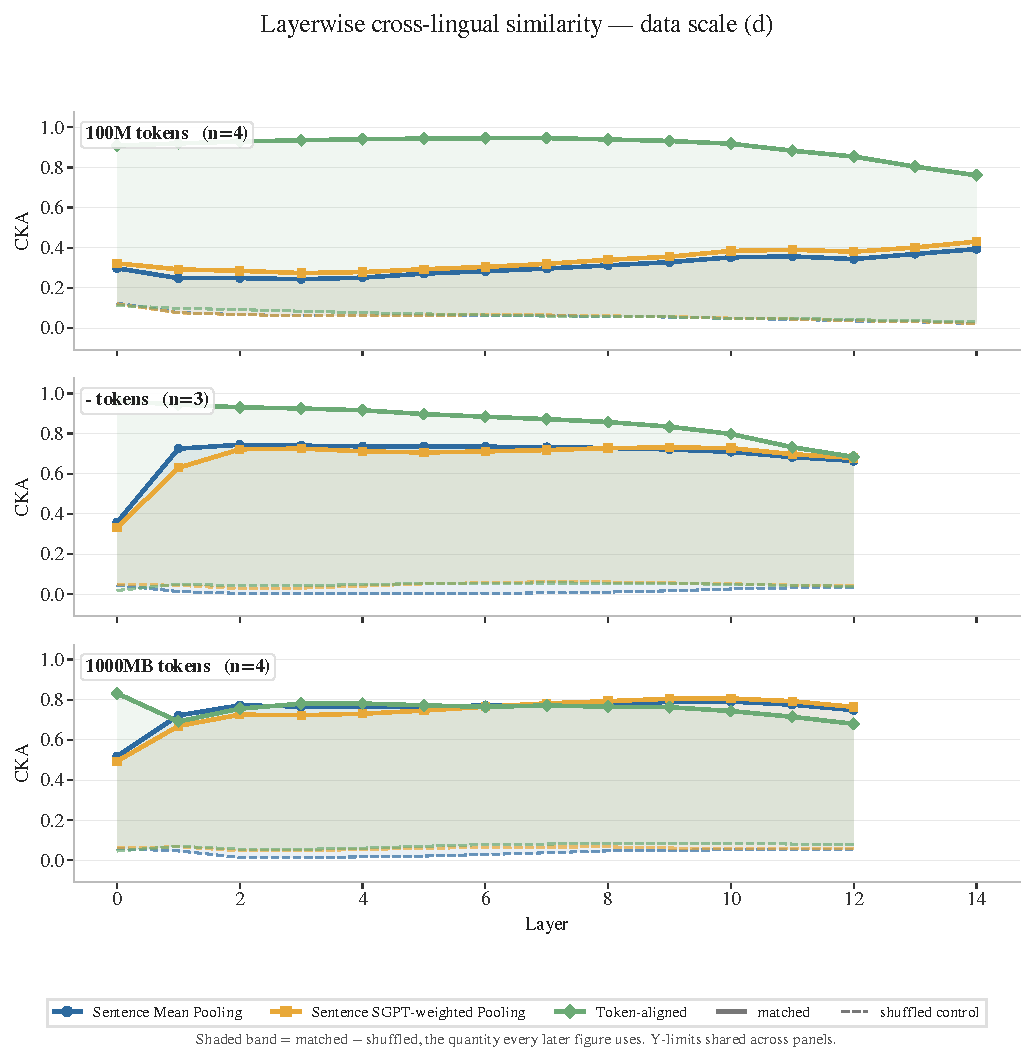
\includegraphics[width=\textwidth,height=0.74\textheight,keepaspectratio]{figures/fig01d_layerwise_cka_families.pdf}
  \end{center}
  \vspace{-0.5em}\begin{center}\tiny {\tiny\texttt{\detokenize{fig01d_layerwise_cka_families.pdf}}}\end{center}
\end{frame}

\subsection{Pairwise CKA across languages}

\begin{frame}{fig02: Pairwise CKA FineWeb-100M 14lang}
  \begin{center}
    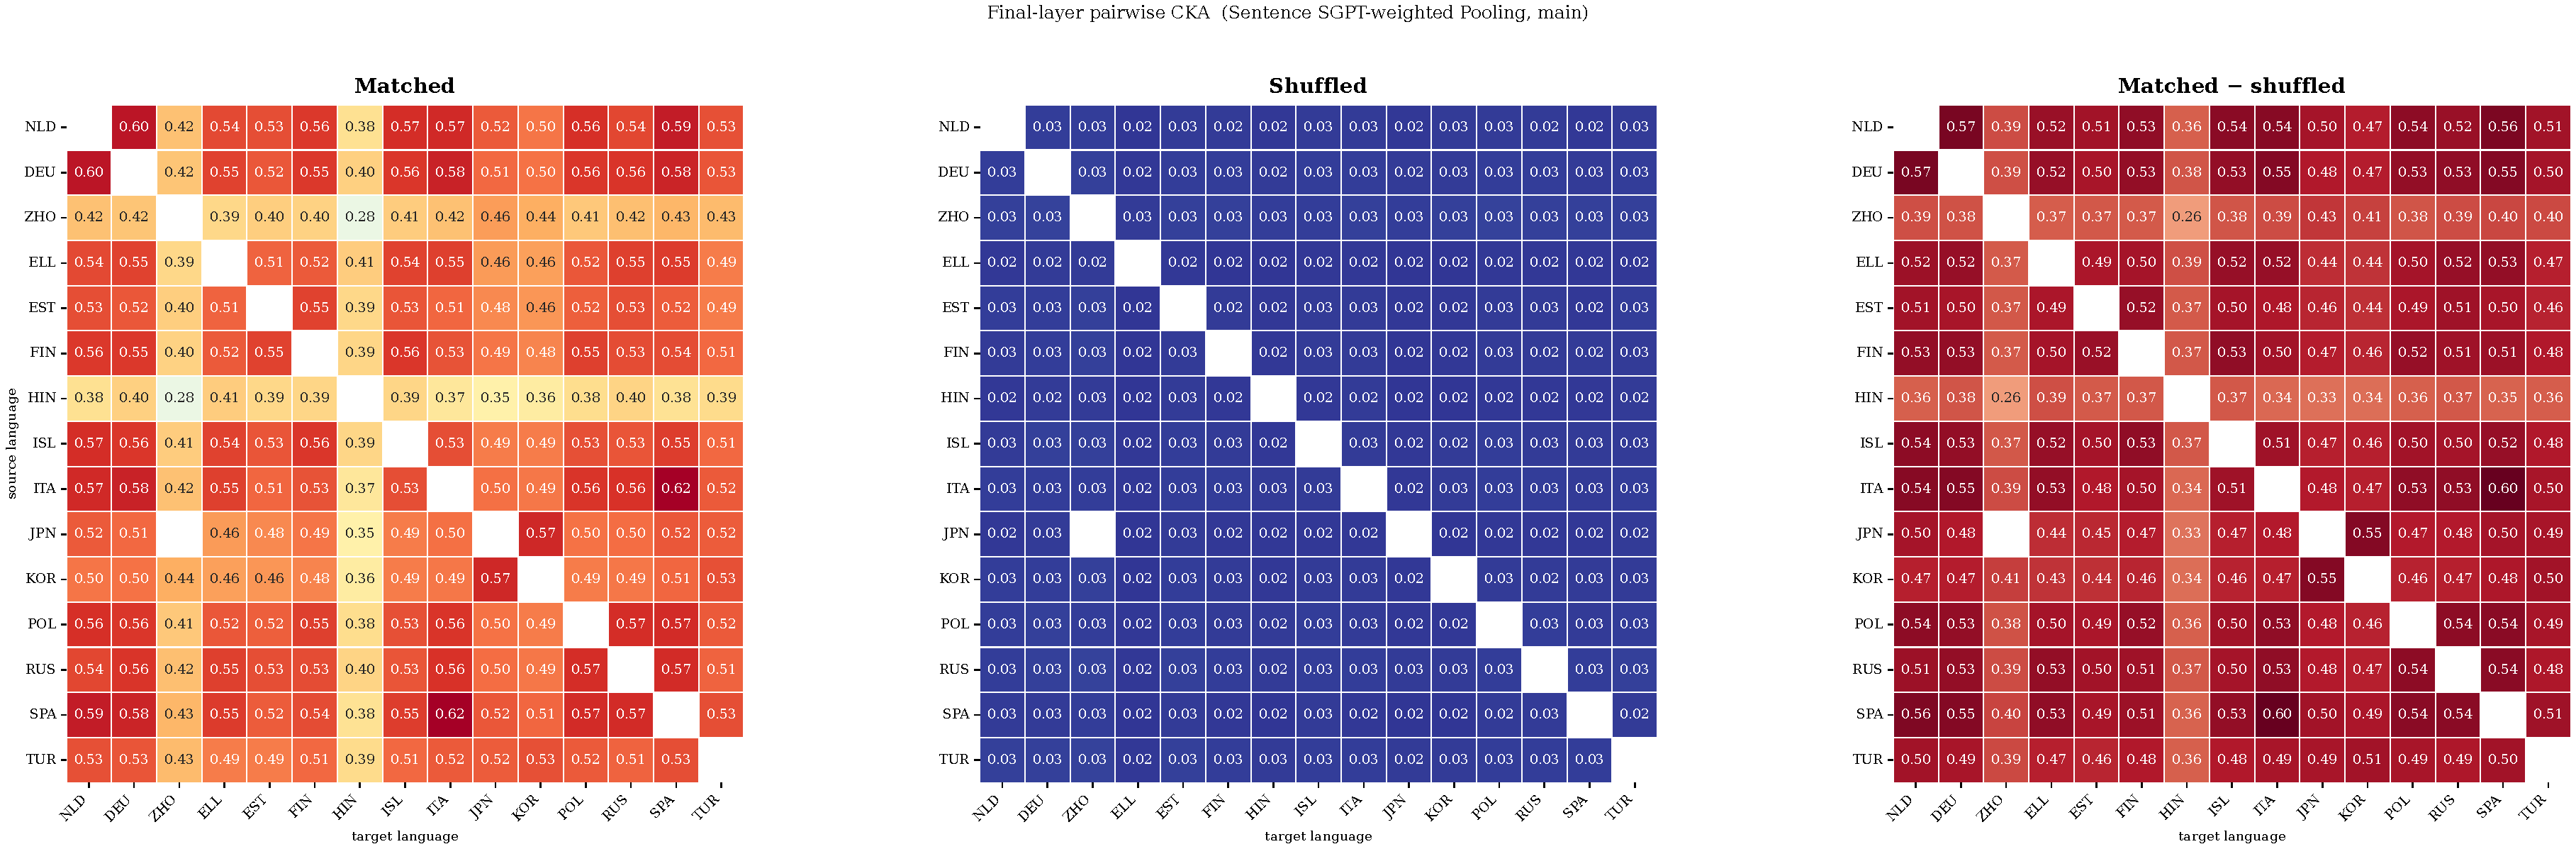
\includegraphics[width=\textwidth,height=0.74\textheight,keepaspectratio]{figures/fig02_pairwise_cka_fw100m_14lang.pdf}
  \end{center}
  \vspace{-0.5em}\begin{center}\tiny {\tiny\texttt{\detokenize{fig02_pairwise_cka_fw100m_14lang.pdf}}}\end{center}
\end{frame}

\begin{frame}{fig02: Pairwise CKA FineWeb-100M 14lang triangular}
  \begin{center}
    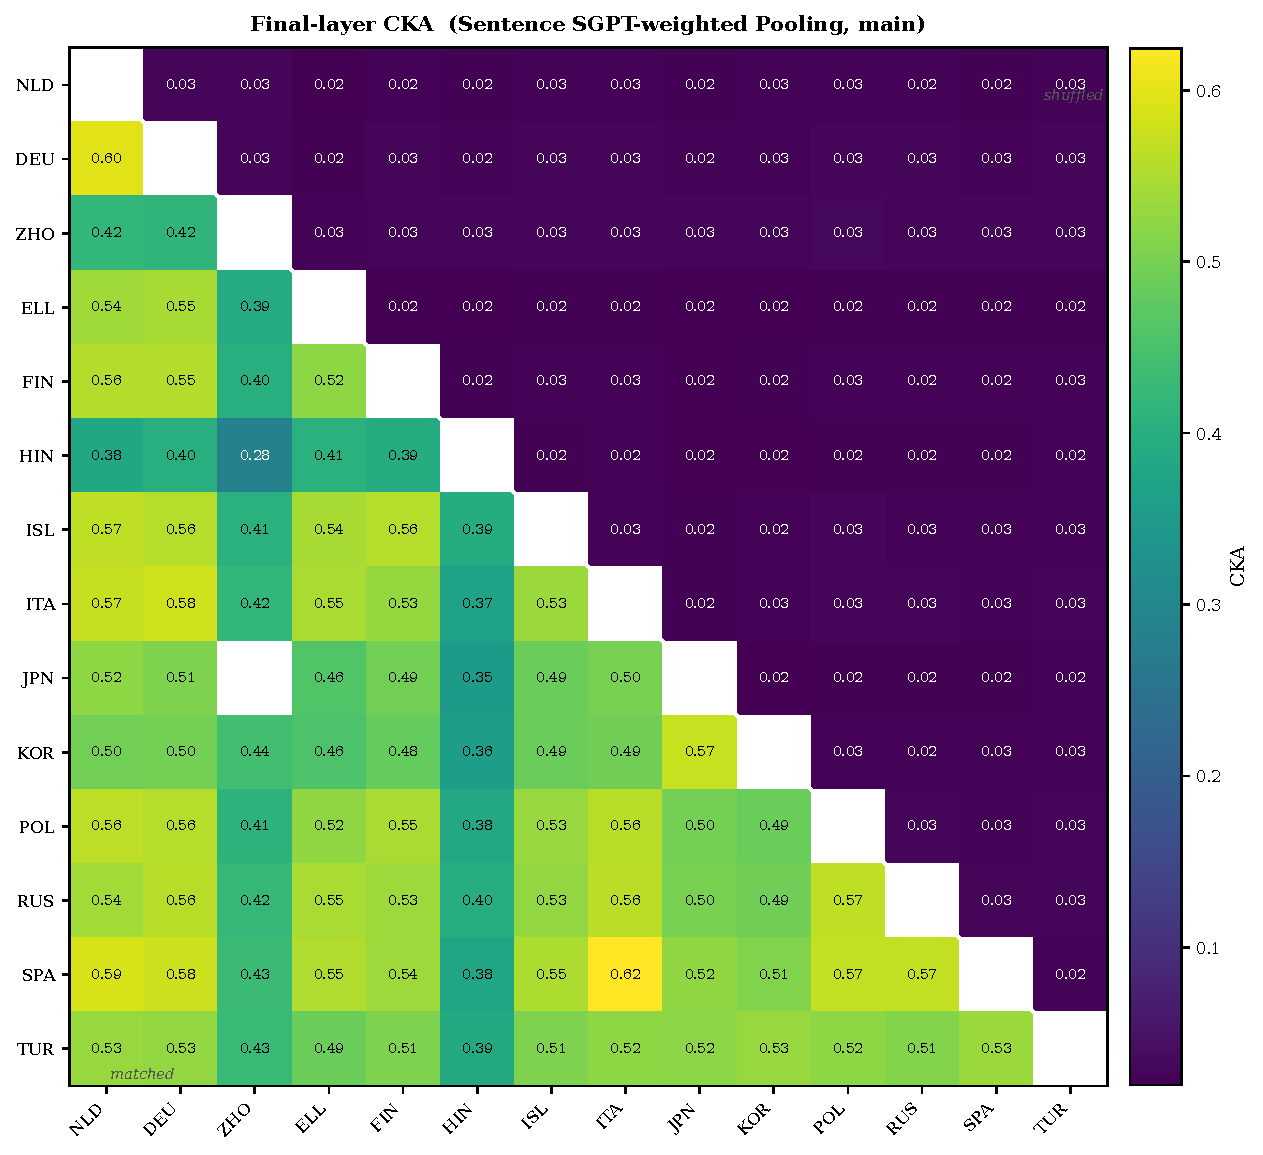
\includegraphics[width=\textwidth,height=0.74\textheight,keepaspectratio]{figures/fig02_pairwise_cka_fw100m_14lang_triangular.pdf}
  \end{center}
  \vspace{-0.5em}\begin{center}\tiny {\tiny\texttt{\detokenize{fig02_pairwise_cka_fw100m_14lang_triangular.pdf}}}\end{center}
\end{frame}

\begin{frame}{fig02: Pairwise CKA main SGPT pooling triangular}
  \begin{center}
    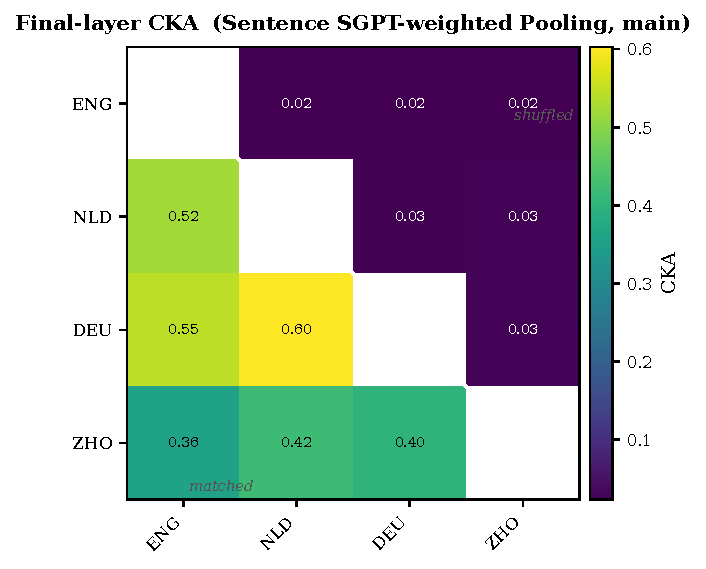
\includegraphics[width=\textwidth,height=0.74\textheight,keepaspectratio]{figures/fig02_pairwise_cka_main_sgpt_triangular.pdf}
  \end{center}
  \vspace{-0.5em}\begin{center}\tiny {\tiny\texttt{\detokenize{fig02_pairwise_cka_main_sgpt_triangular.pdf}}}\end{center}
\end{frame}

\begin{frame}{fig02: Pairwise CKA main SGPT pooling triptych}
  \begin{center}
    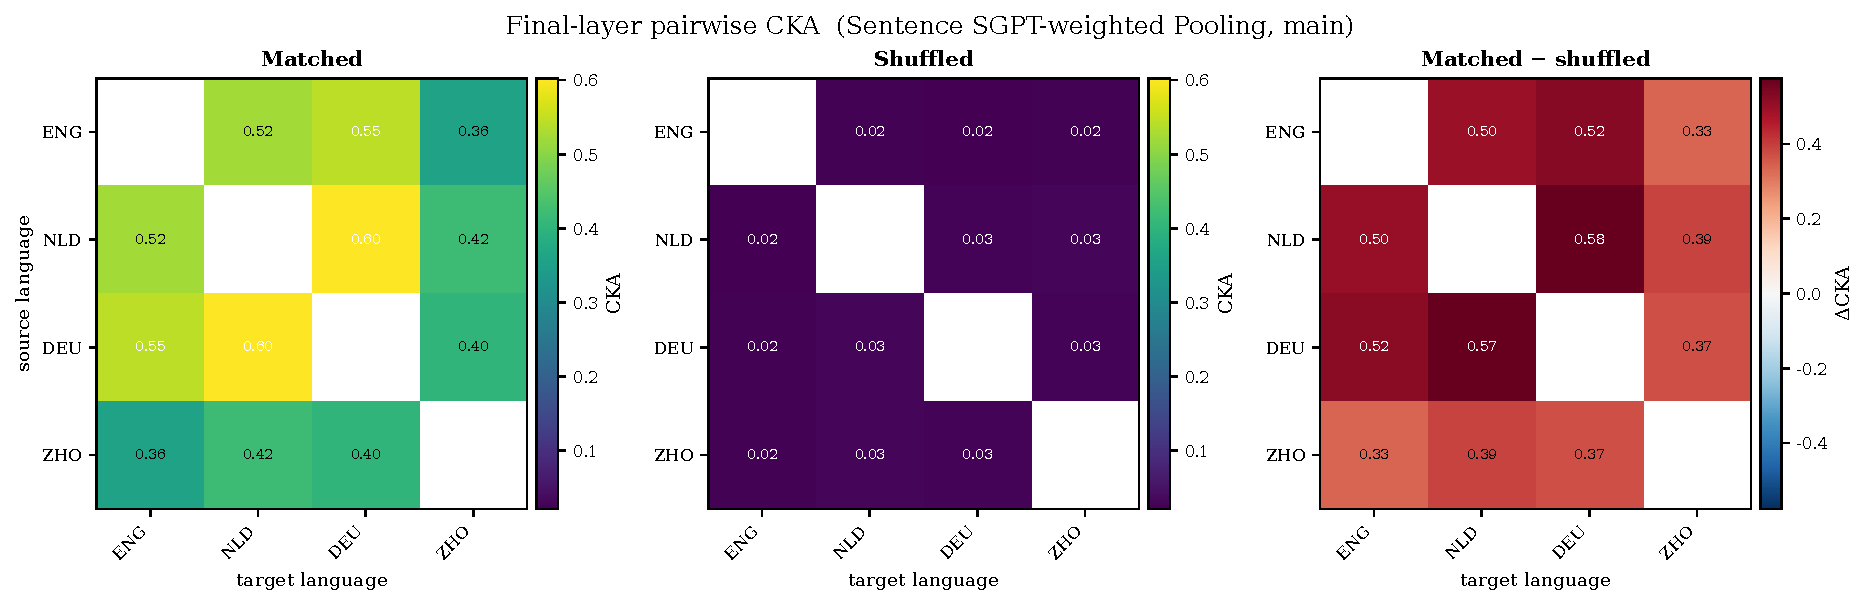
\includegraphics[width=\textwidth,height=0.74\textheight,keepaspectratio]{figures/fig02_pairwise_cka_main_sgpt_triptych.pdf}
  \end{center}
  \vspace{-0.5em}\begin{center}\tiny {\tiny\texttt{\detokenize{fig02_pairwise_cka_main_sgpt_triptych.pdf}}}\end{center}
\end{frame}

\subsection{Training scale}

\begin{frame}{fig03: Training scale humanscale}
  \begin{center}
    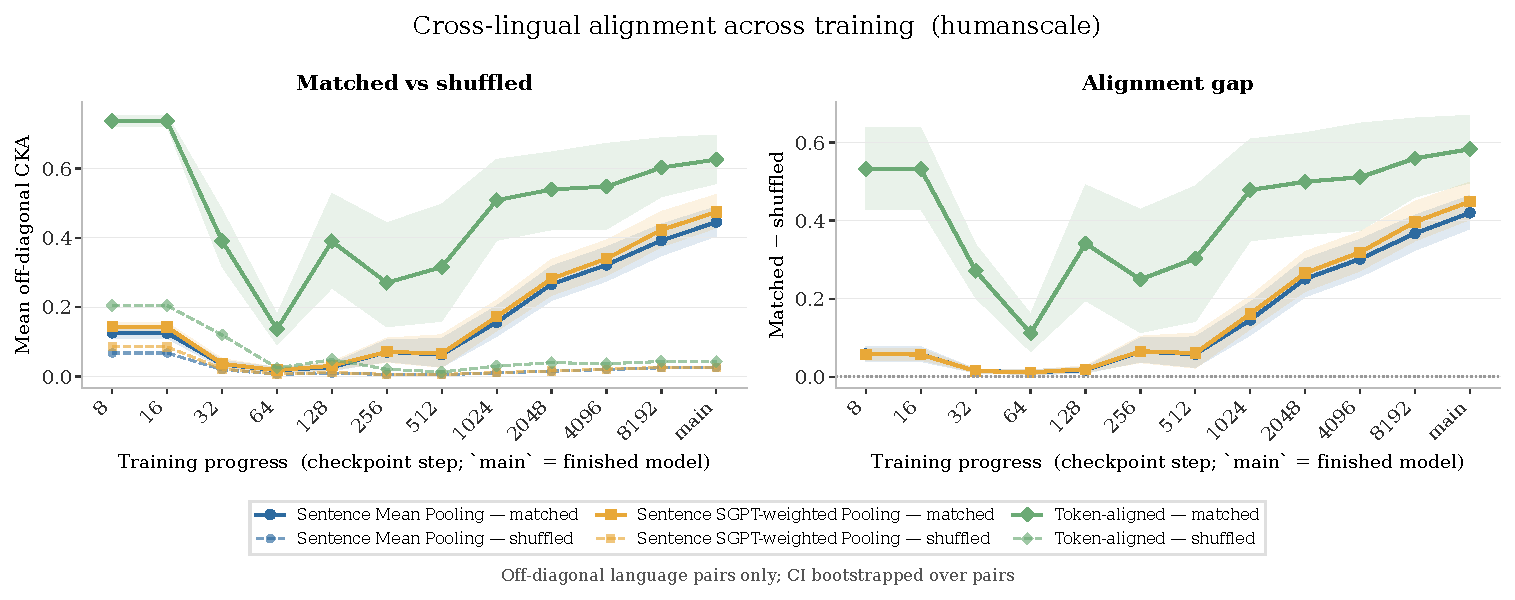
\includegraphics[width=\textwidth,height=0.74\textheight,keepaspectratio]{figures/fig03_training_scale_humanscale.pdf}
  \end{center}
  \vspace{-0.5em}\begin{center}\tiny {\tiny\texttt{\detokenize{fig03_training_scale_humanscale.pdf}}}\end{center}
\end{frame}

\subsection{Cross-size comparisons}

\begin{frame}{fig04: Crosssize mean pool}
  \begin{center}
    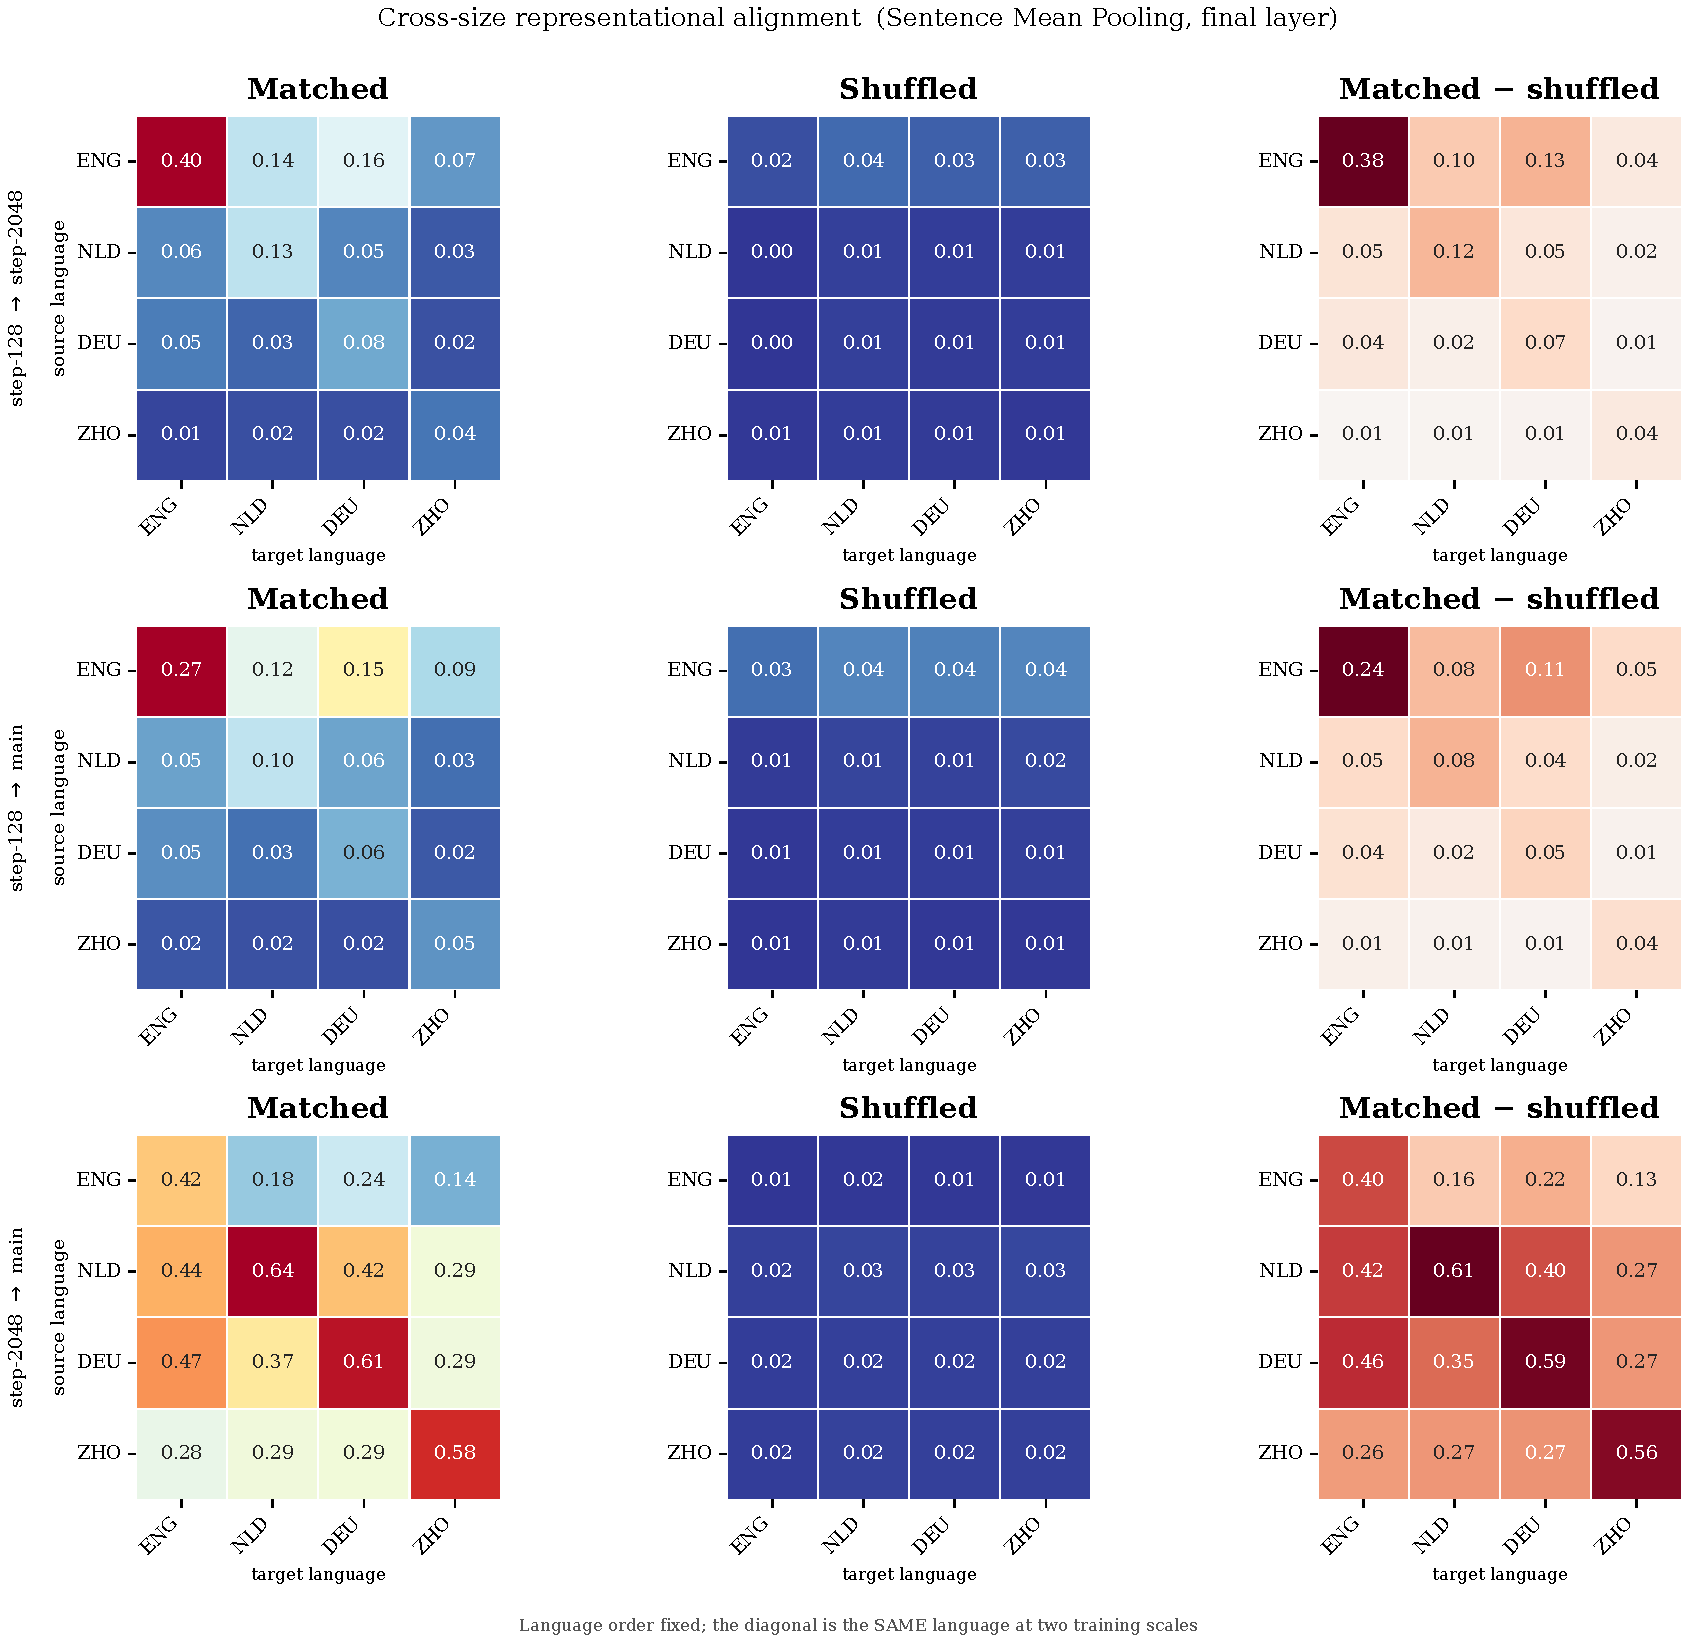
\includegraphics[width=\textwidth,height=0.74\textheight,keepaspectratio]{figures/fig04_crosssize_mean_pool.pdf}
  \end{center}
  \vspace{-0.5em}\begin{center}\tiny {\tiny\texttt{\detokenize{fig04_crosssize_mean_pool.pdf}}}\end{center}
\end{frame}

\begin{frame}{fig04: Crosssize SGPT pooling}
  \begin{center}
    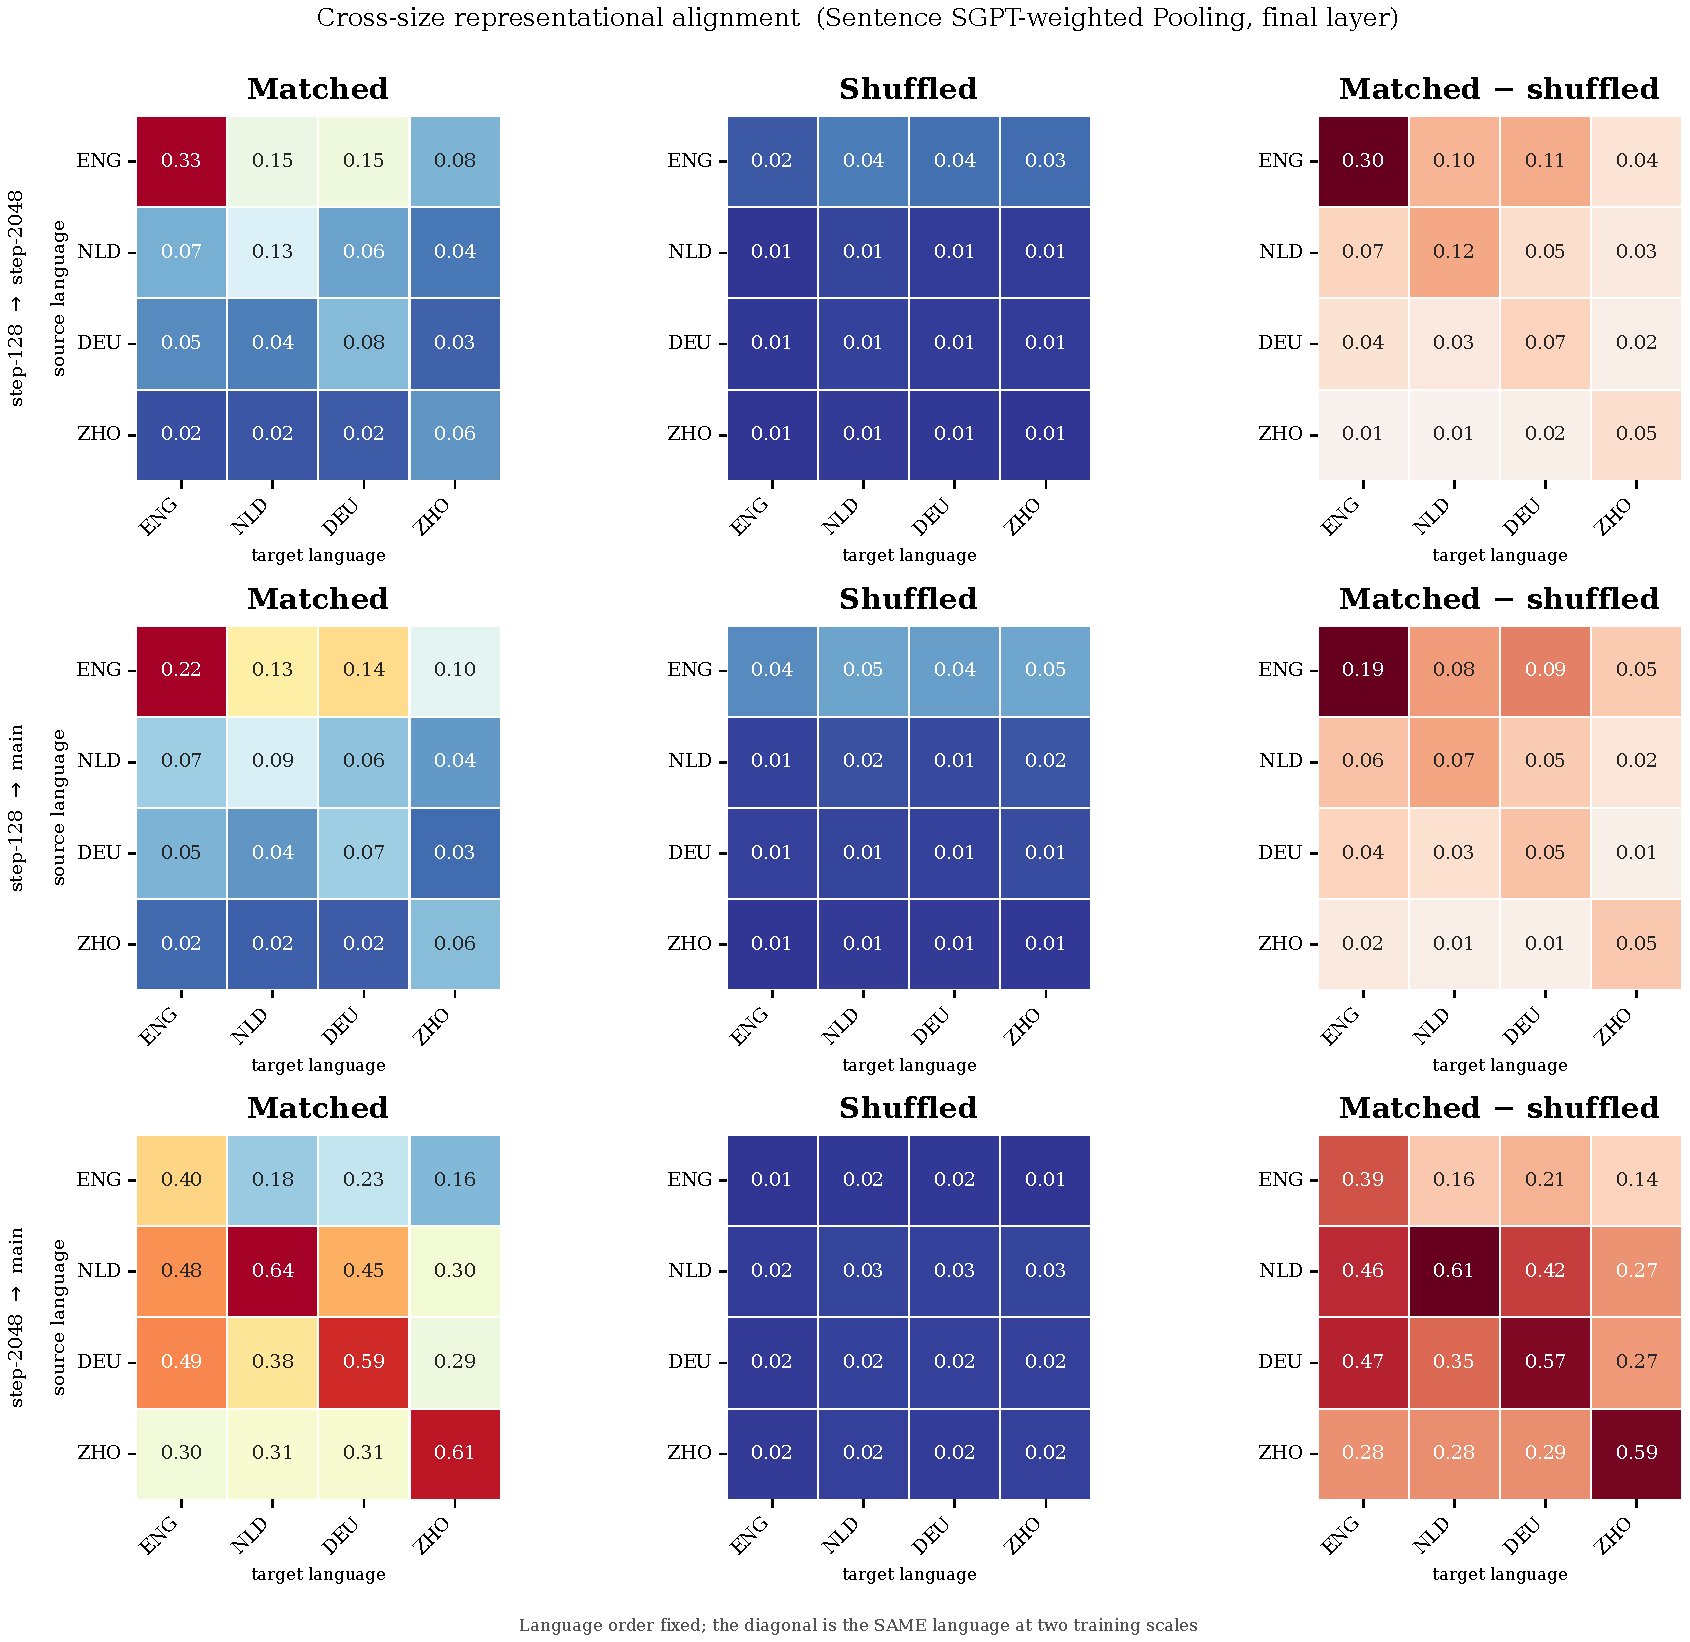
\includegraphics[width=\textwidth,height=0.74\textheight,keepaspectratio]{figures/fig04_crosssize_sgpt.pdf}
  \end{center}
  \vspace{-0.5em}\begin{center}\tiny {\tiny\texttt{\detokenize{fig04_crosssize_sgpt.pdf}}}\end{center}
\end{frame}

\begin{frame}{fig04: Crosssize token aligned}
  \begin{center}
    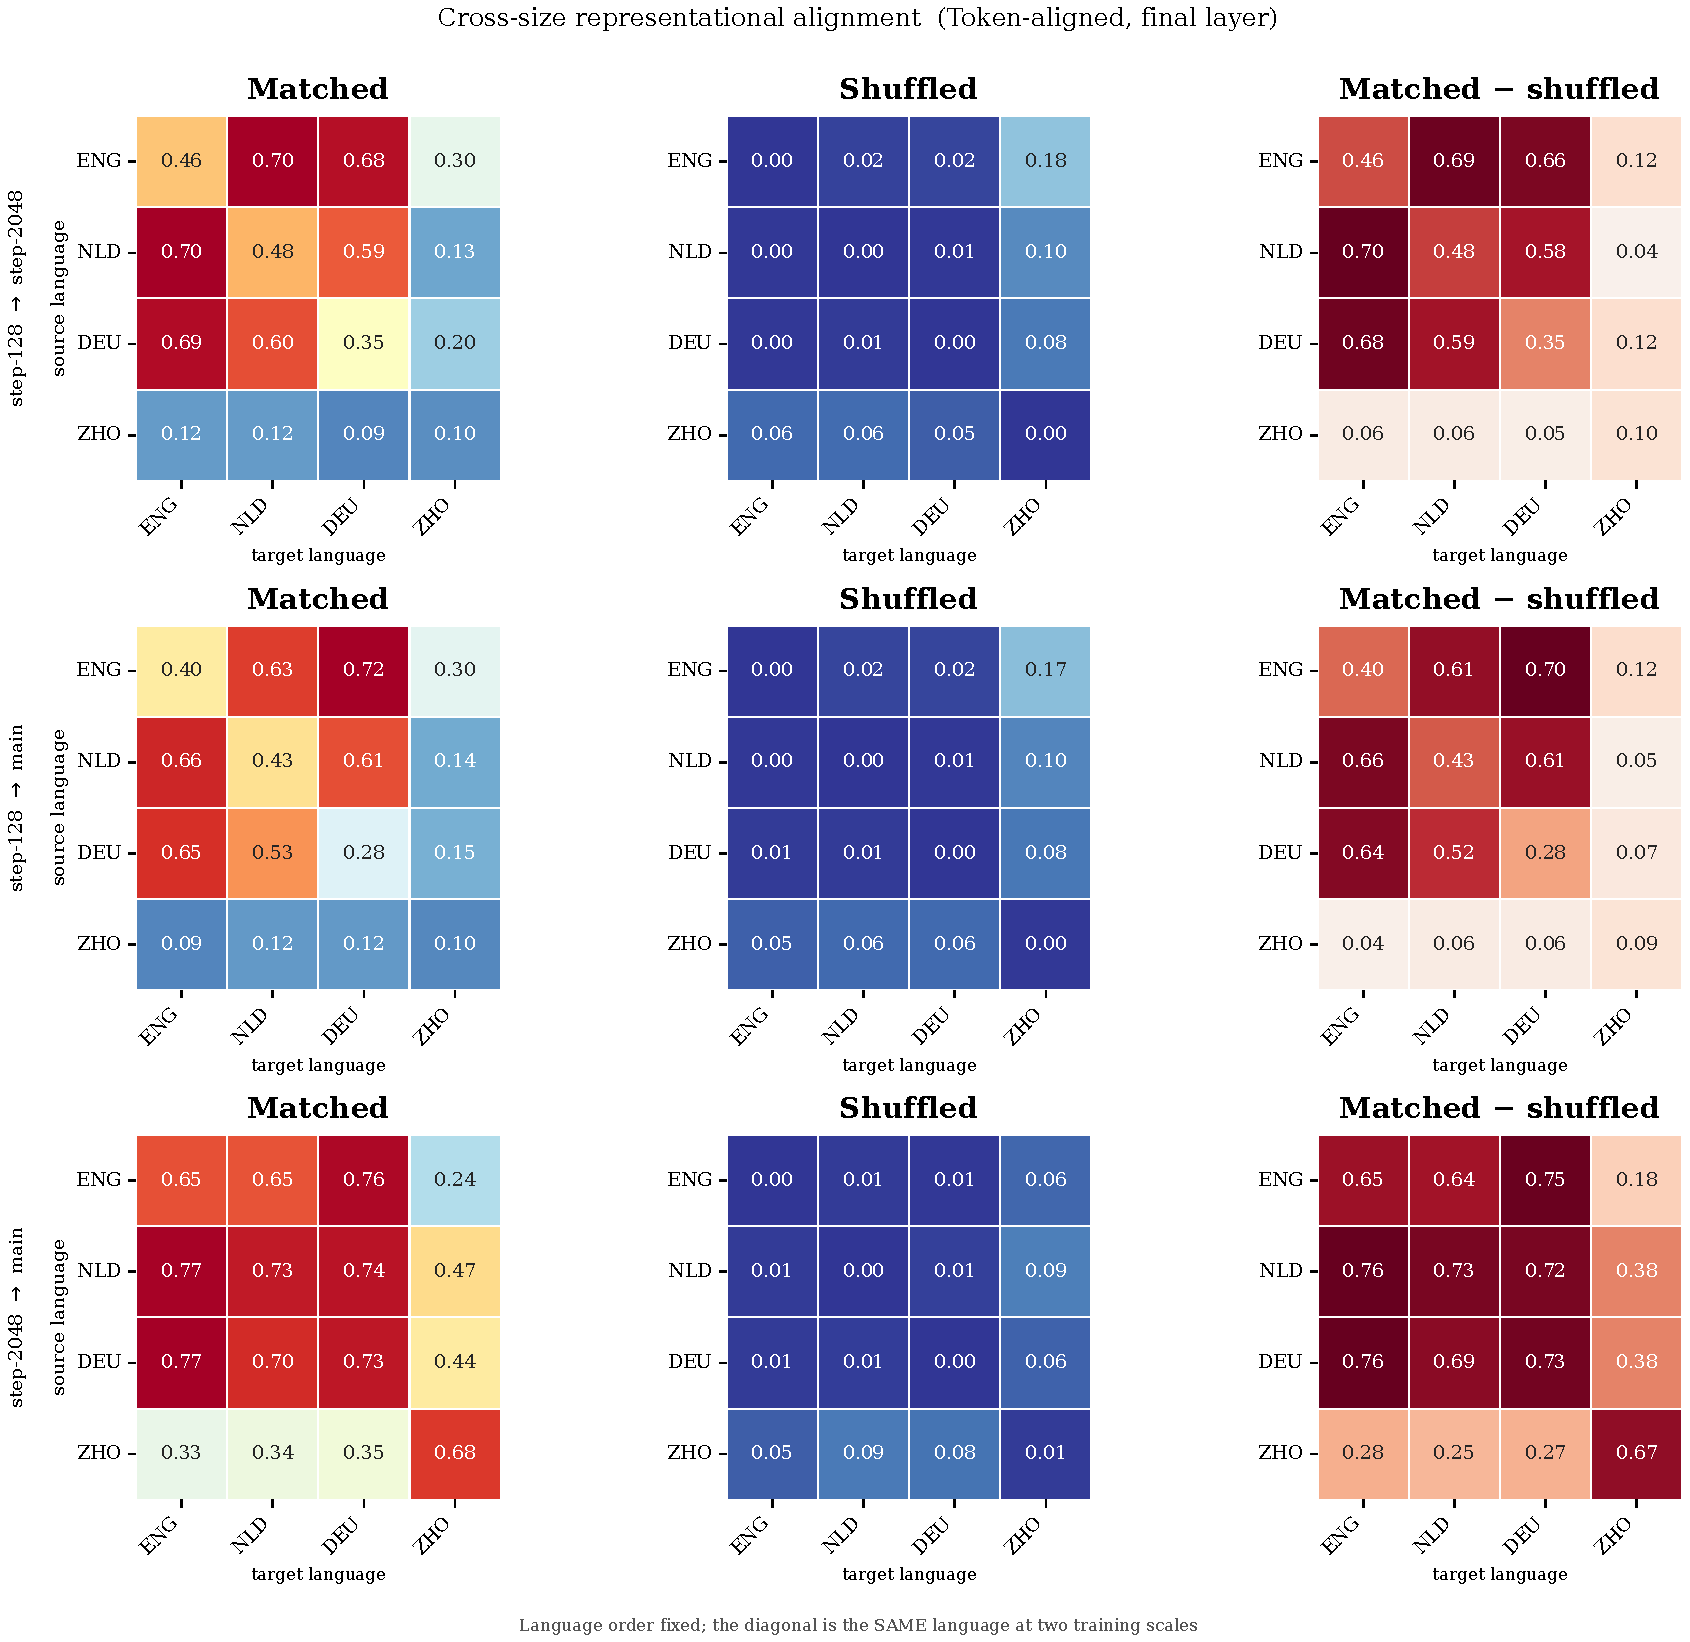
\includegraphics[width=\textwidth,height=0.74\textheight,keepaspectratio]{figures/fig04_crosssize_token_aligned.pdf}
  \end{center}
  \vspace{-0.5em}\begin{center}\tiny {\tiny\texttt{\detokenize{fig04_crosssize_token_aligned.pdf}}}\end{center}
\end{frame}

\subsection{Model families}

\begin{frame}{fig05: Families SGPT pooling delta}
  \begin{center}
    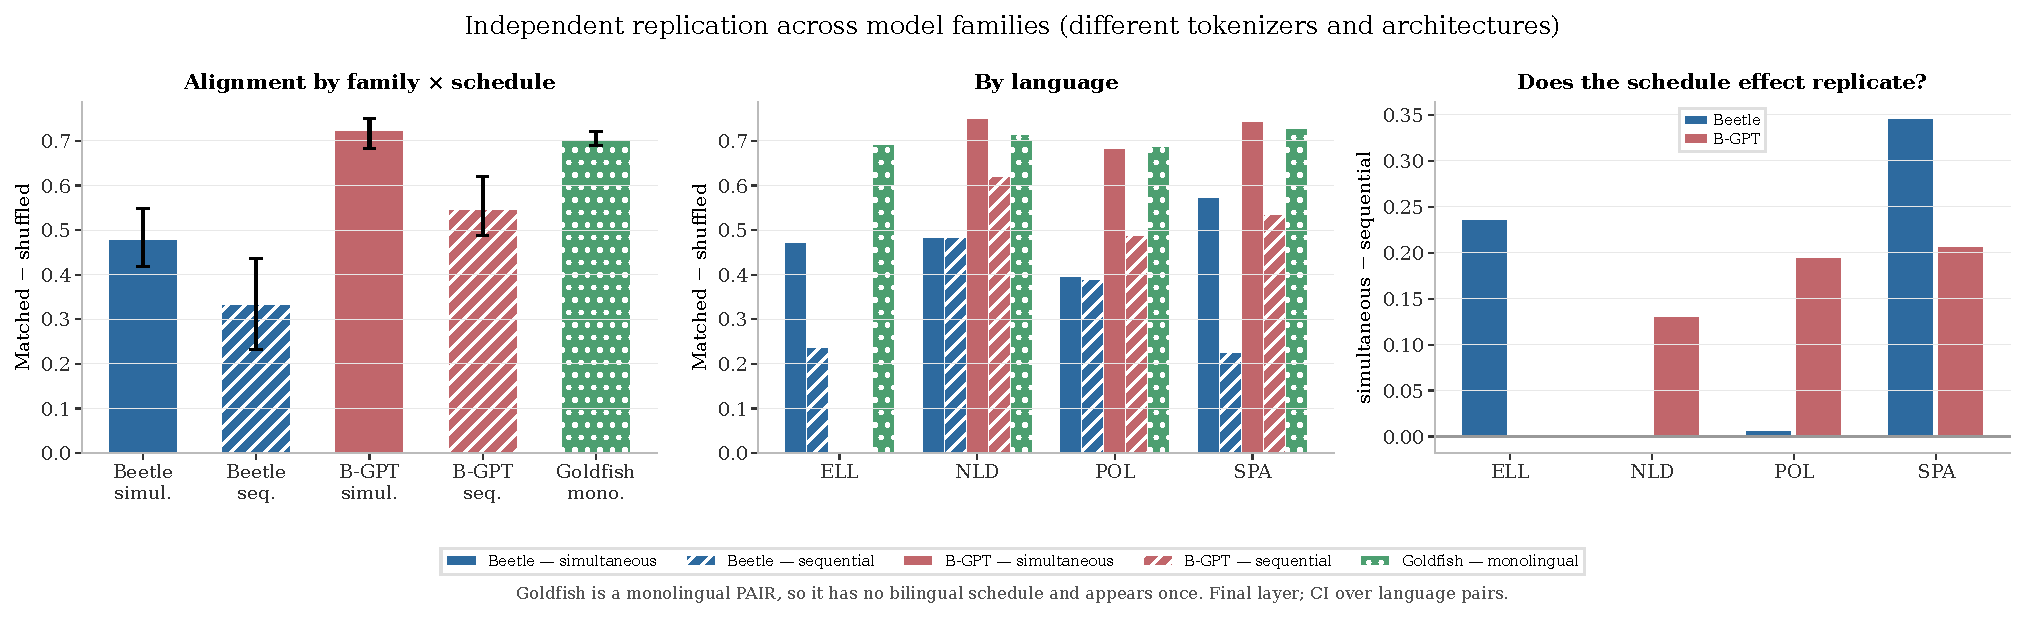
\includegraphics[width=\textwidth,height=0.74\textheight,keepaspectratio]{figures/fig05_families_sgpt_delta.pdf}
  \end{center}
  \vspace{-0.5em}\begin{center}\tiny {\tiny\texttt{\detokenize{fig05_families_sgpt_delta.pdf}}}\end{center}
\end{frame}

\subsection{Reconstruction}

\begin{frame}{fig07: Reconstruction bilingual}
  \begin{center}
    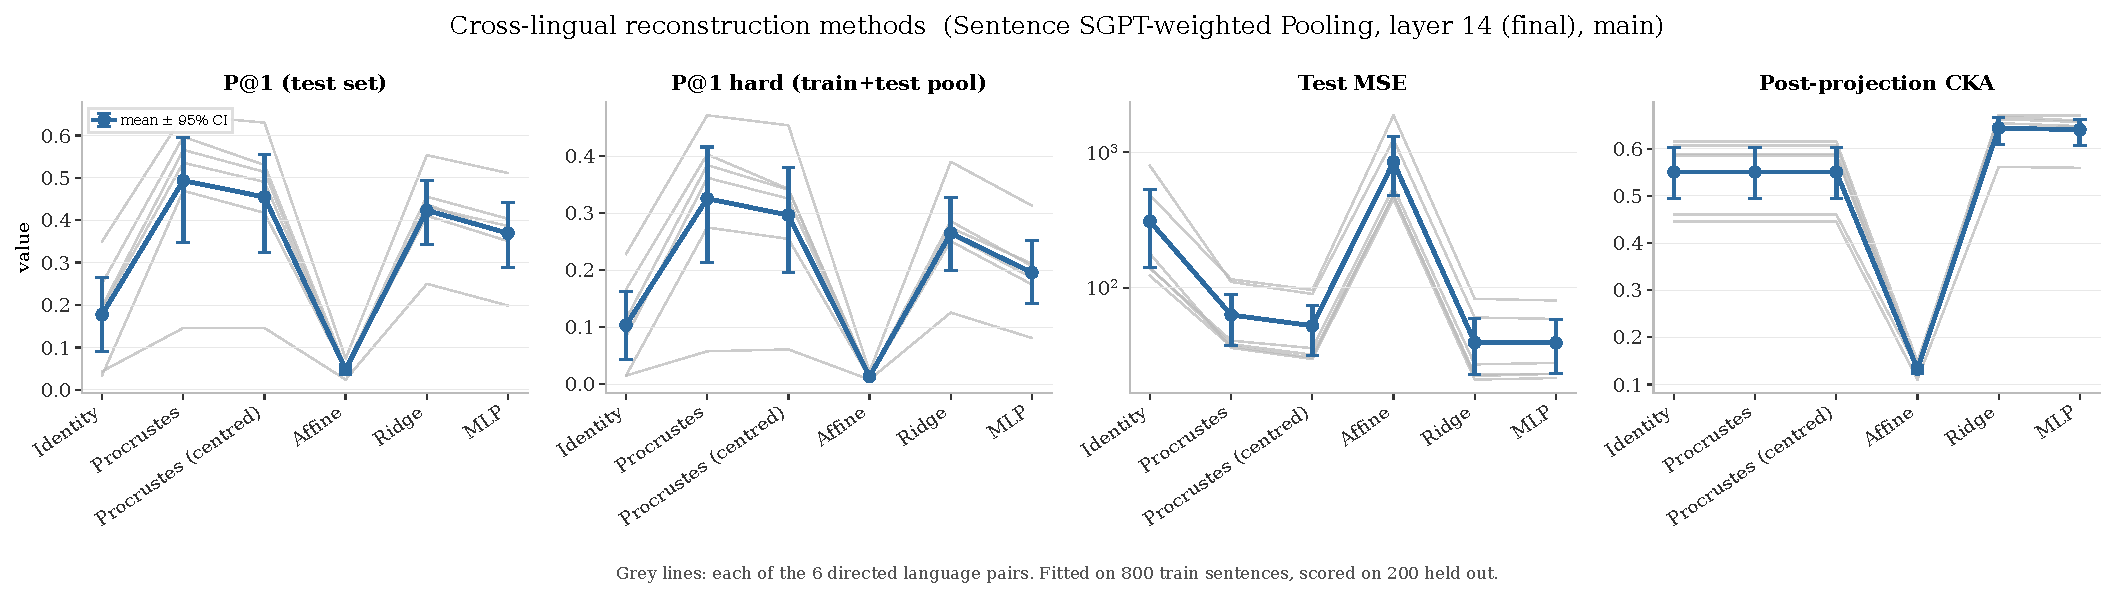
\includegraphics[width=\textwidth,height=0.74\textheight,keepaspectratio]{figures/fig07_reconstruction_bilingual.pdf}
  \end{center}
  \vspace{-0.5em}\begin{center}\tiny {\tiny\texttt{\detokenize{fig07_reconstruction_bilingual.pdf}}}\end{center}
\end{frame}

\begin{frame}{fig07: Reconstruction methods SGPT pooling final}
  \begin{center}
    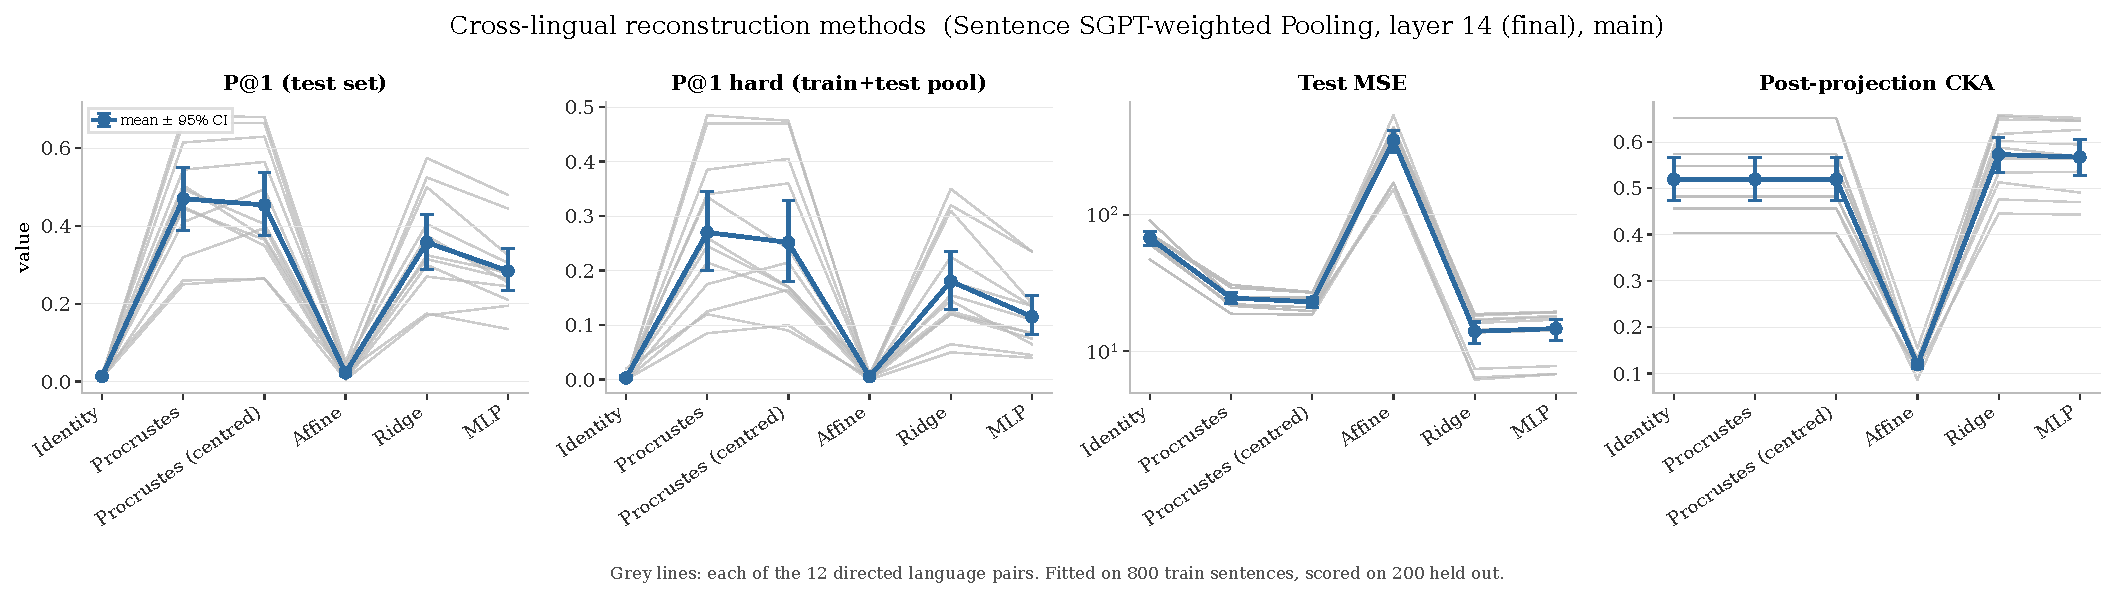
\includegraphics[width=\textwidth,height=0.74\textheight,keepaspectratio]{figures/fig07_reconstruction_methods_sgpt_final.pdf}
  \end{center}
  \vspace{-0.5em}\begin{center}\tiny {\tiny\texttt{\detokenize{fig07_reconstruction_methods_sgpt_final.pdf}}}\end{center}
\end{frame}

\subsection{Procrustes vs affine and ridge}

\begin{frame}{fig08: Procrustes vs affine}
  \begin{center}
    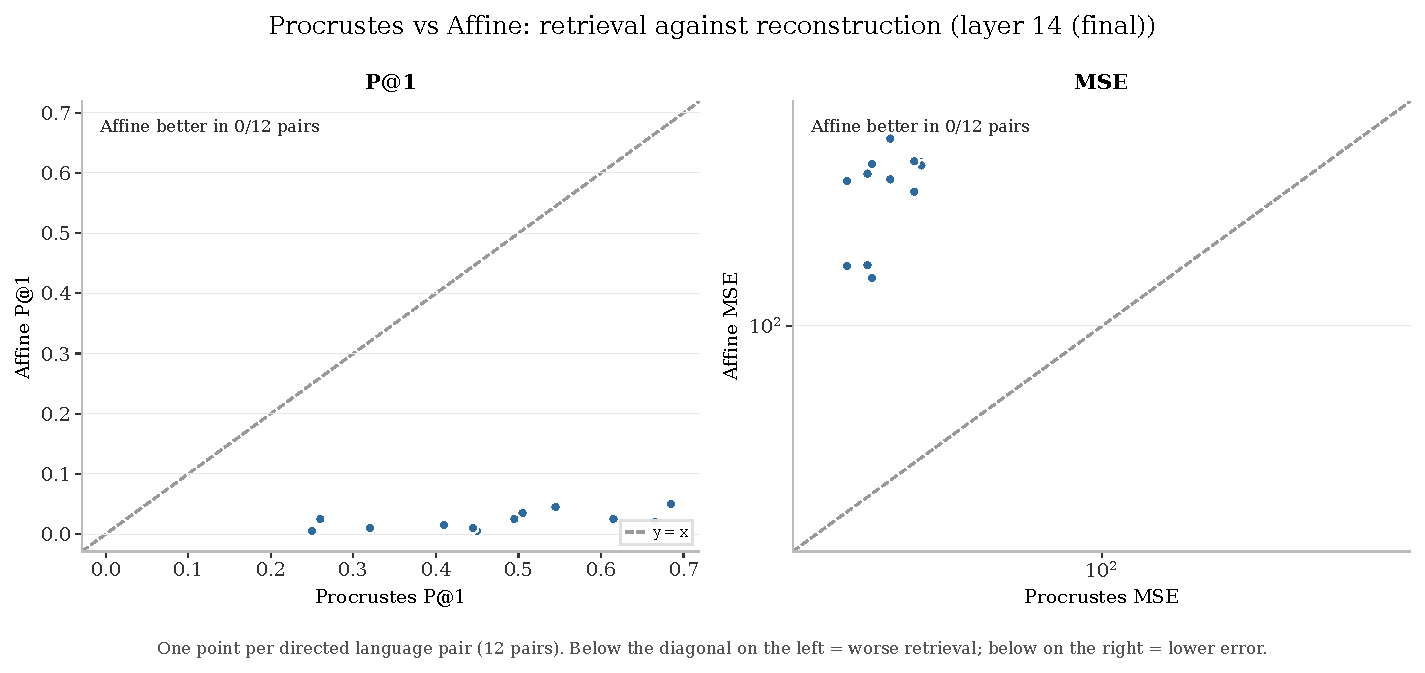
\includegraphics[width=\textwidth,height=0.74\textheight,keepaspectratio]{figures/fig08_procrustes_vs_affine.pdf}
  \end{center}
  \vspace{-0.5em}\begin{center}\tiny {\tiny\texttt{\detokenize{fig08_procrustes_vs_affine.pdf}}}\end{center}
\end{frame}

\begin{frame}{fig08: Procrustes vs ridge}
  \begin{center}
    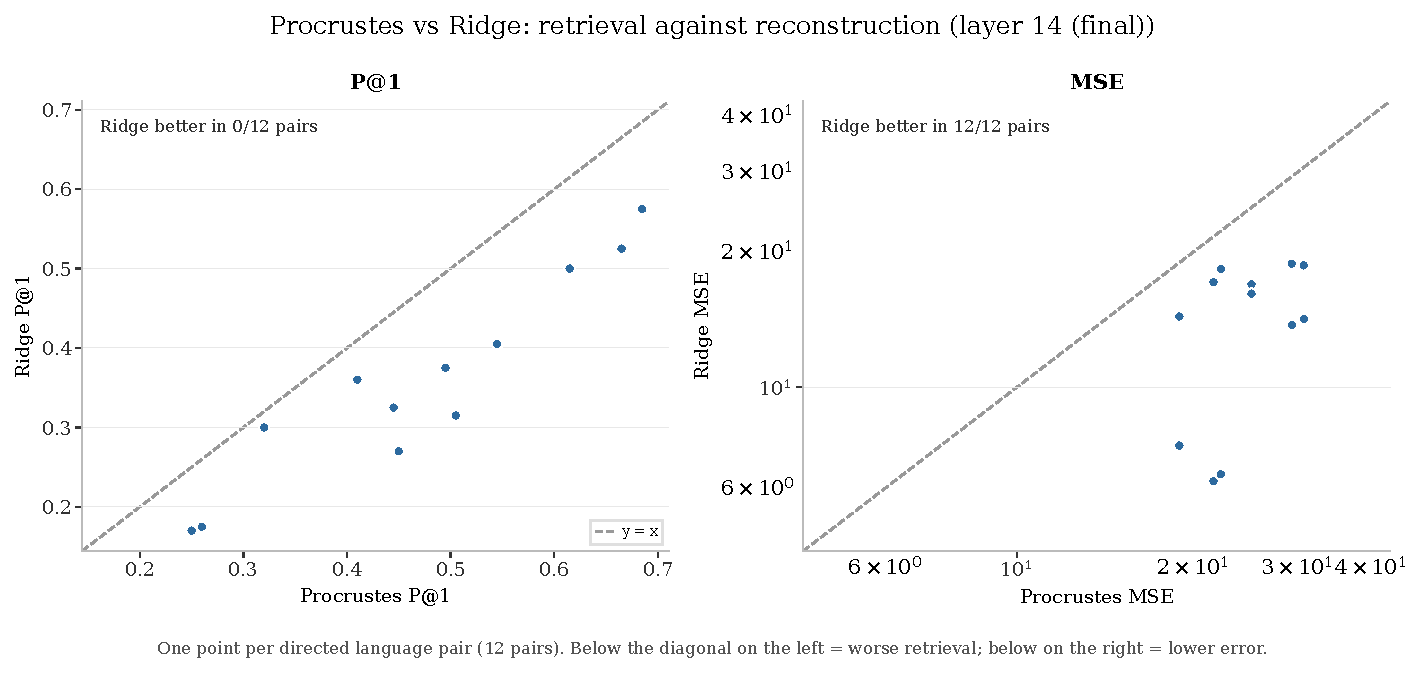
\includegraphics[width=\textwidth,height=0.74\textheight,keepaspectratio]{figures/fig08_procrustes_vs_ridge.pdf}
  \end{center}
  \vspace{-0.5em}\begin{center}\tiny {\tiny\texttt{\detokenize{fig08_procrustes_vs_ridge.pdf}}}\end{center}
\end{frame}

\subsection{Layer-wise Procrustes retrieval}

\begin{frame}{fig09: Layerwise procrustes p at 1 bilingual}
  \begin{center}
    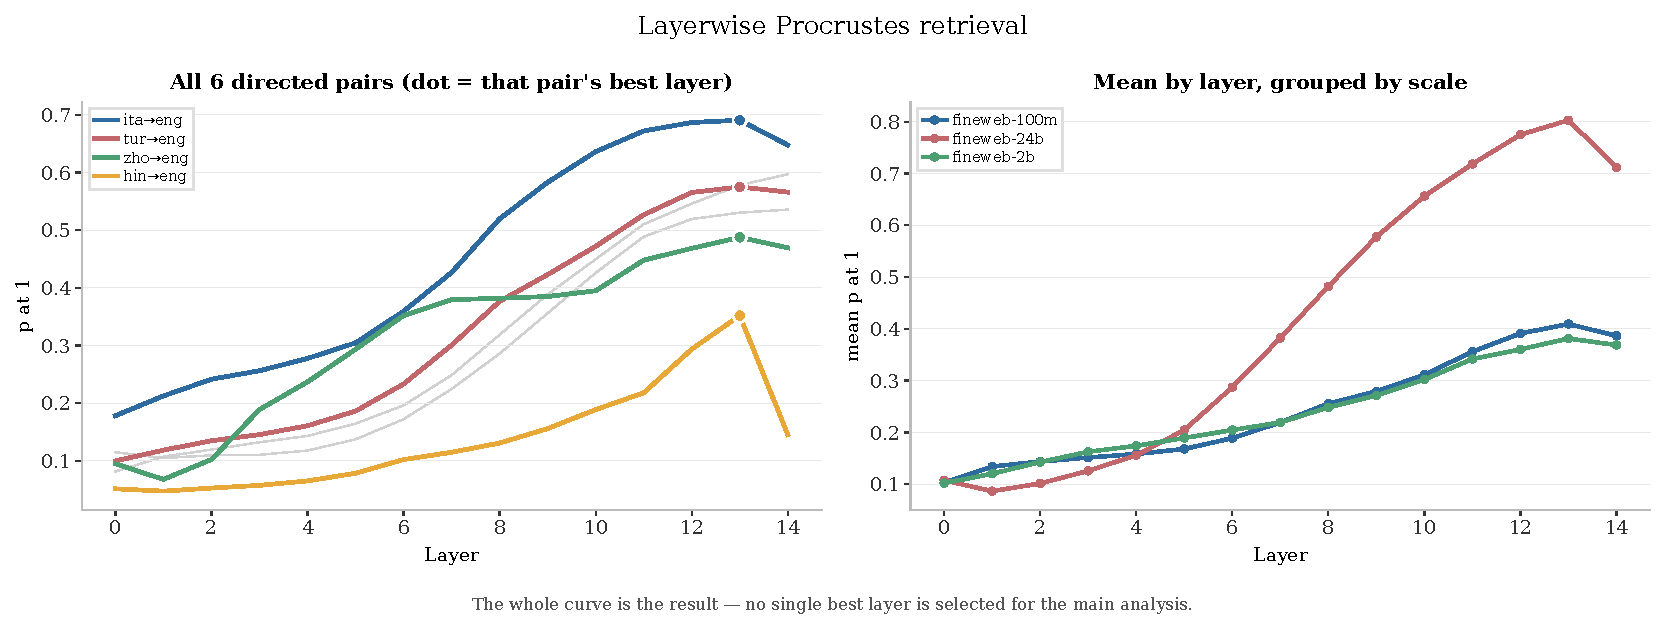
\includegraphics[width=\textwidth,height=0.74\textheight,keepaspectratio]{figures/fig09_layerwise_procrustes_p_at_1_bilingual.pdf}
  \end{center}
  \vspace{-0.5em}\begin{center}\tiny {\tiny\texttt{\detokenize{fig09_layerwise_procrustes_p_at_1_bilingual.pdf}}}\end{center}
\end{frame}

\begin{frame}{fig09: Layerwise procrustes p at 1 mono}
  \begin{center}
    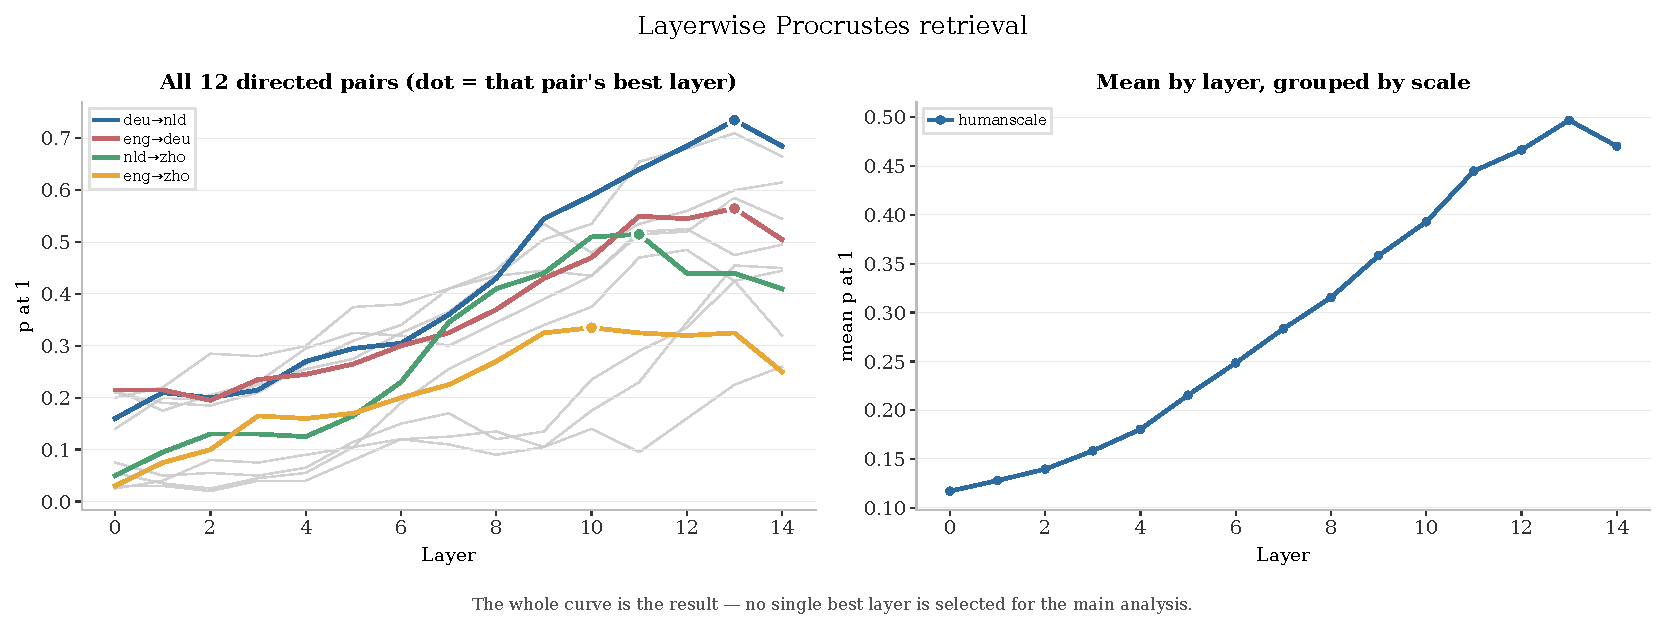
\includegraphics[width=\textwidth,height=0.74\textheight,keepaspectratio]{figures/fig09_layerwise_procrustes_p_at_1_mono.pdf}
  \end{center}
  \vspace{-0.5em}\begin{center}\tiny {\tiny\texttt{\detokenize{fig09_layerwise_procrustes_p_at_1_mono.pdf}}}\end{center}
\end{frame}

\subsection{Method x metric x layer}

\begin{frame}{fig10: Method metric layer bilingual}
  \begin{center}
    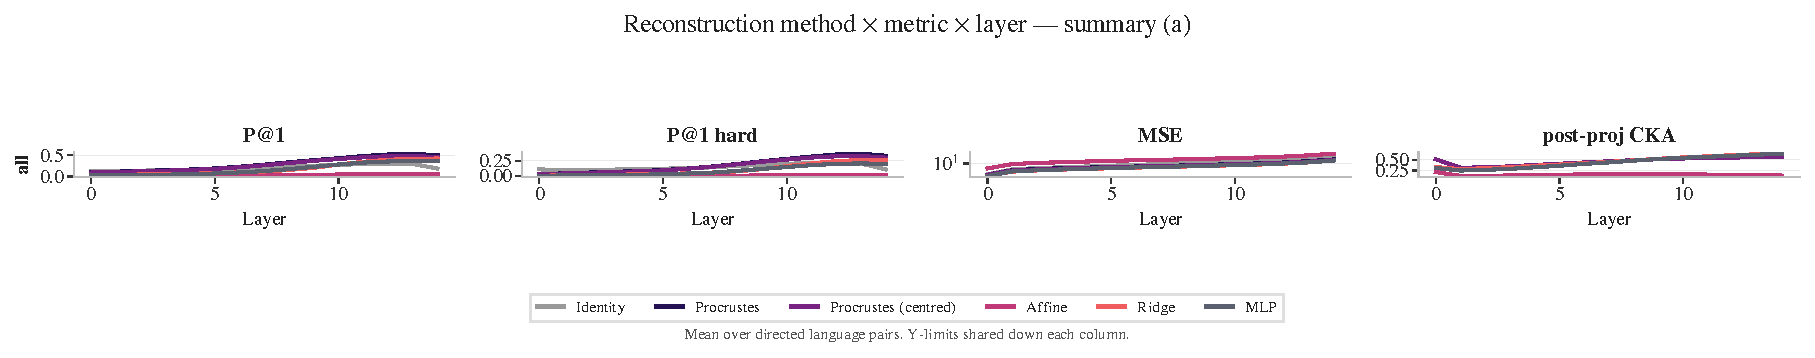
\includegraphics[width=\textwidth,height=0.74\textheight,keepaspectratio]{figures/fig10a_method_metric_layer_bilingual.pdf}
  \end{center}
  \vspace{-0.5em}\begin{center}\tiny {\tiny\texttt{\detokenize{fig10a_method_metric_layer_bilingual.pdf}}}\end{center}
\end{frame}

\begin{frame}{fig10: Method metric layer mono}
  \begin{center}
    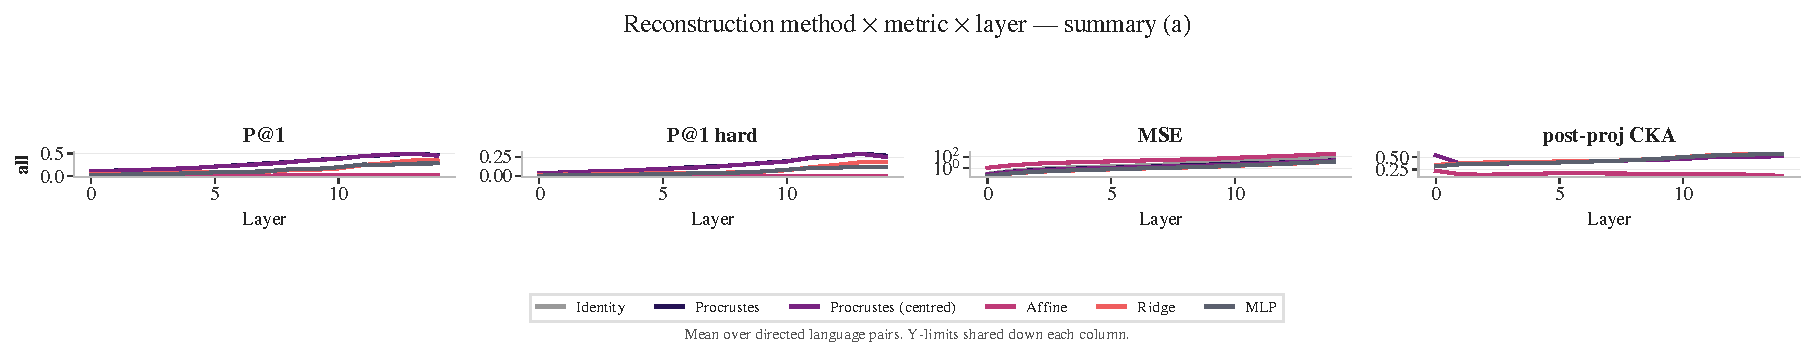
\includegraphics[width=\textwidth,height=0.74\textheight,keepaspectratio]{figures/fig10a_method_metric_layer_mono.pdf}
  \end{center}
  \vspace{-0.5em}\begin{center}\tiny {\tiny\texttt{\detokenize{fig10a_method_metric_layer_mono.pdf}}}\end{center}
\end{frame}

\begin{frame}{fig10: Method metric layer bilingual}
  \begin{center}
    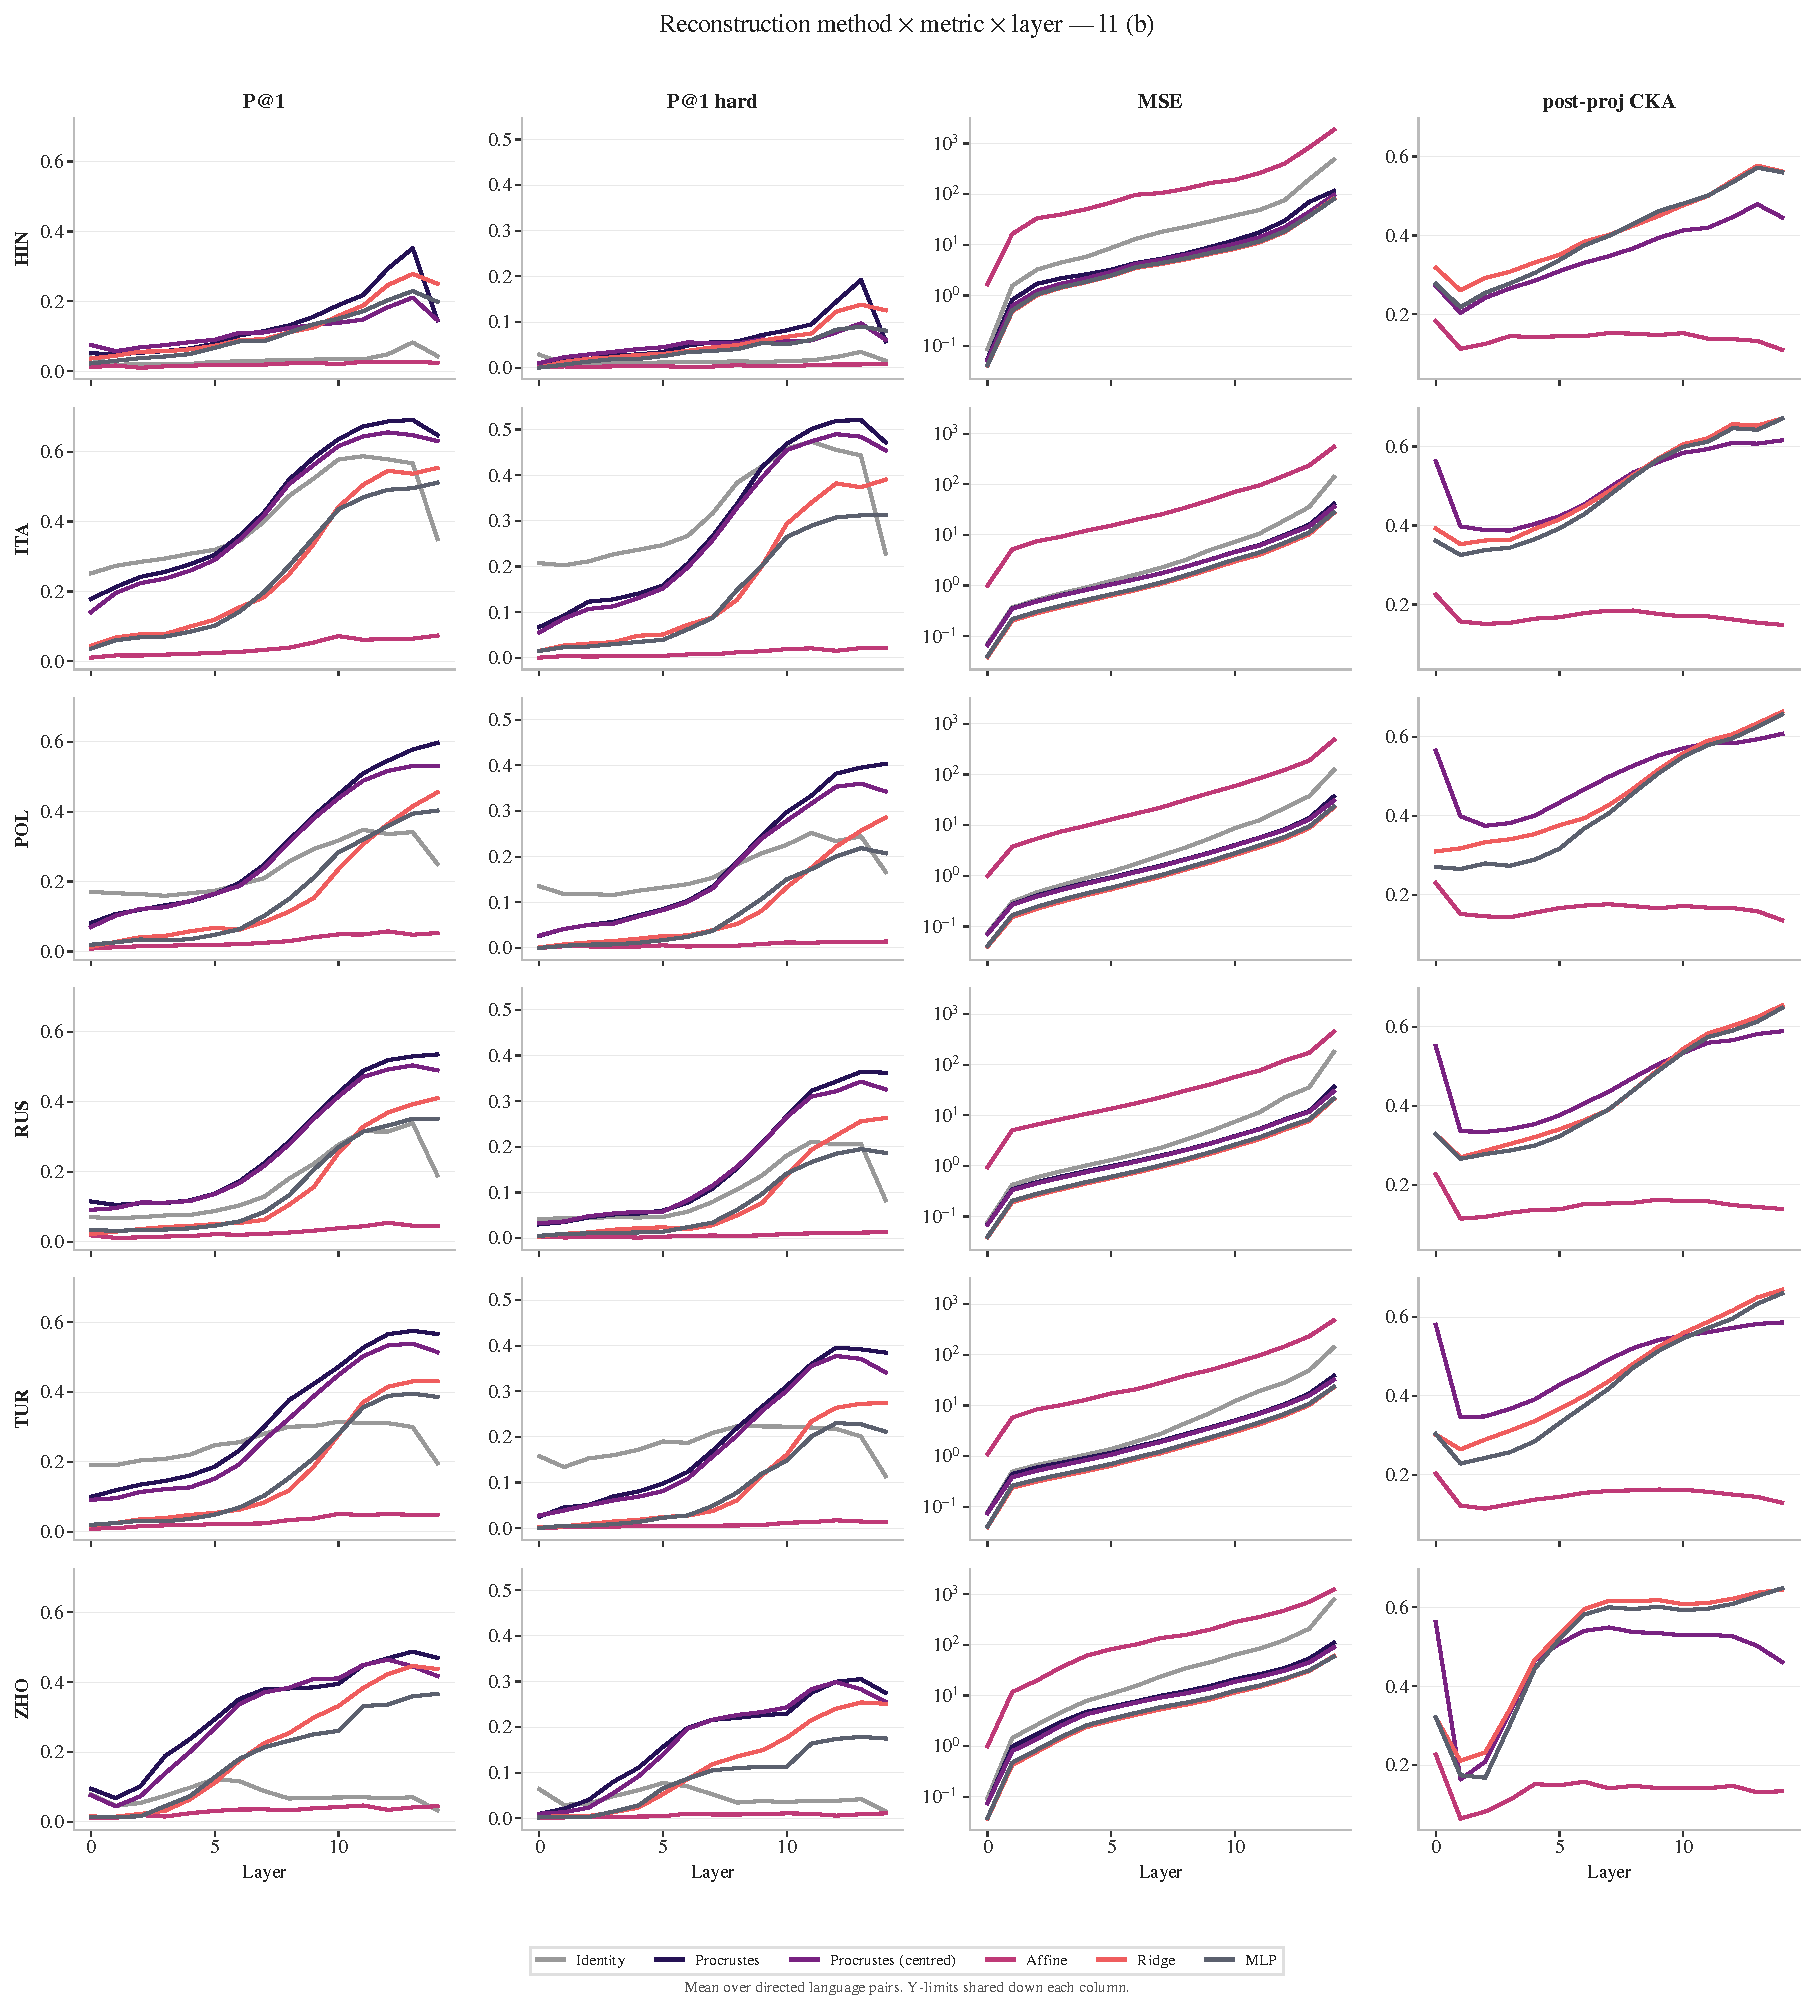
\includegraphics[width=\textwidth,height=0.74\textheight,keepaspectratio]{figures/fig10b_method_metric_layer_bilingual.pdf}
  \end{center}
  \vspace{-0.5em}\begin{center}\tiny {\tiny\texttt{\detokenize{fig10b_method_metric_layer_bilingual.pdf}}}\end{center}
\end{frame}

\begin{frame}{fig10: Method metric layer mono}
  \begin{center}
    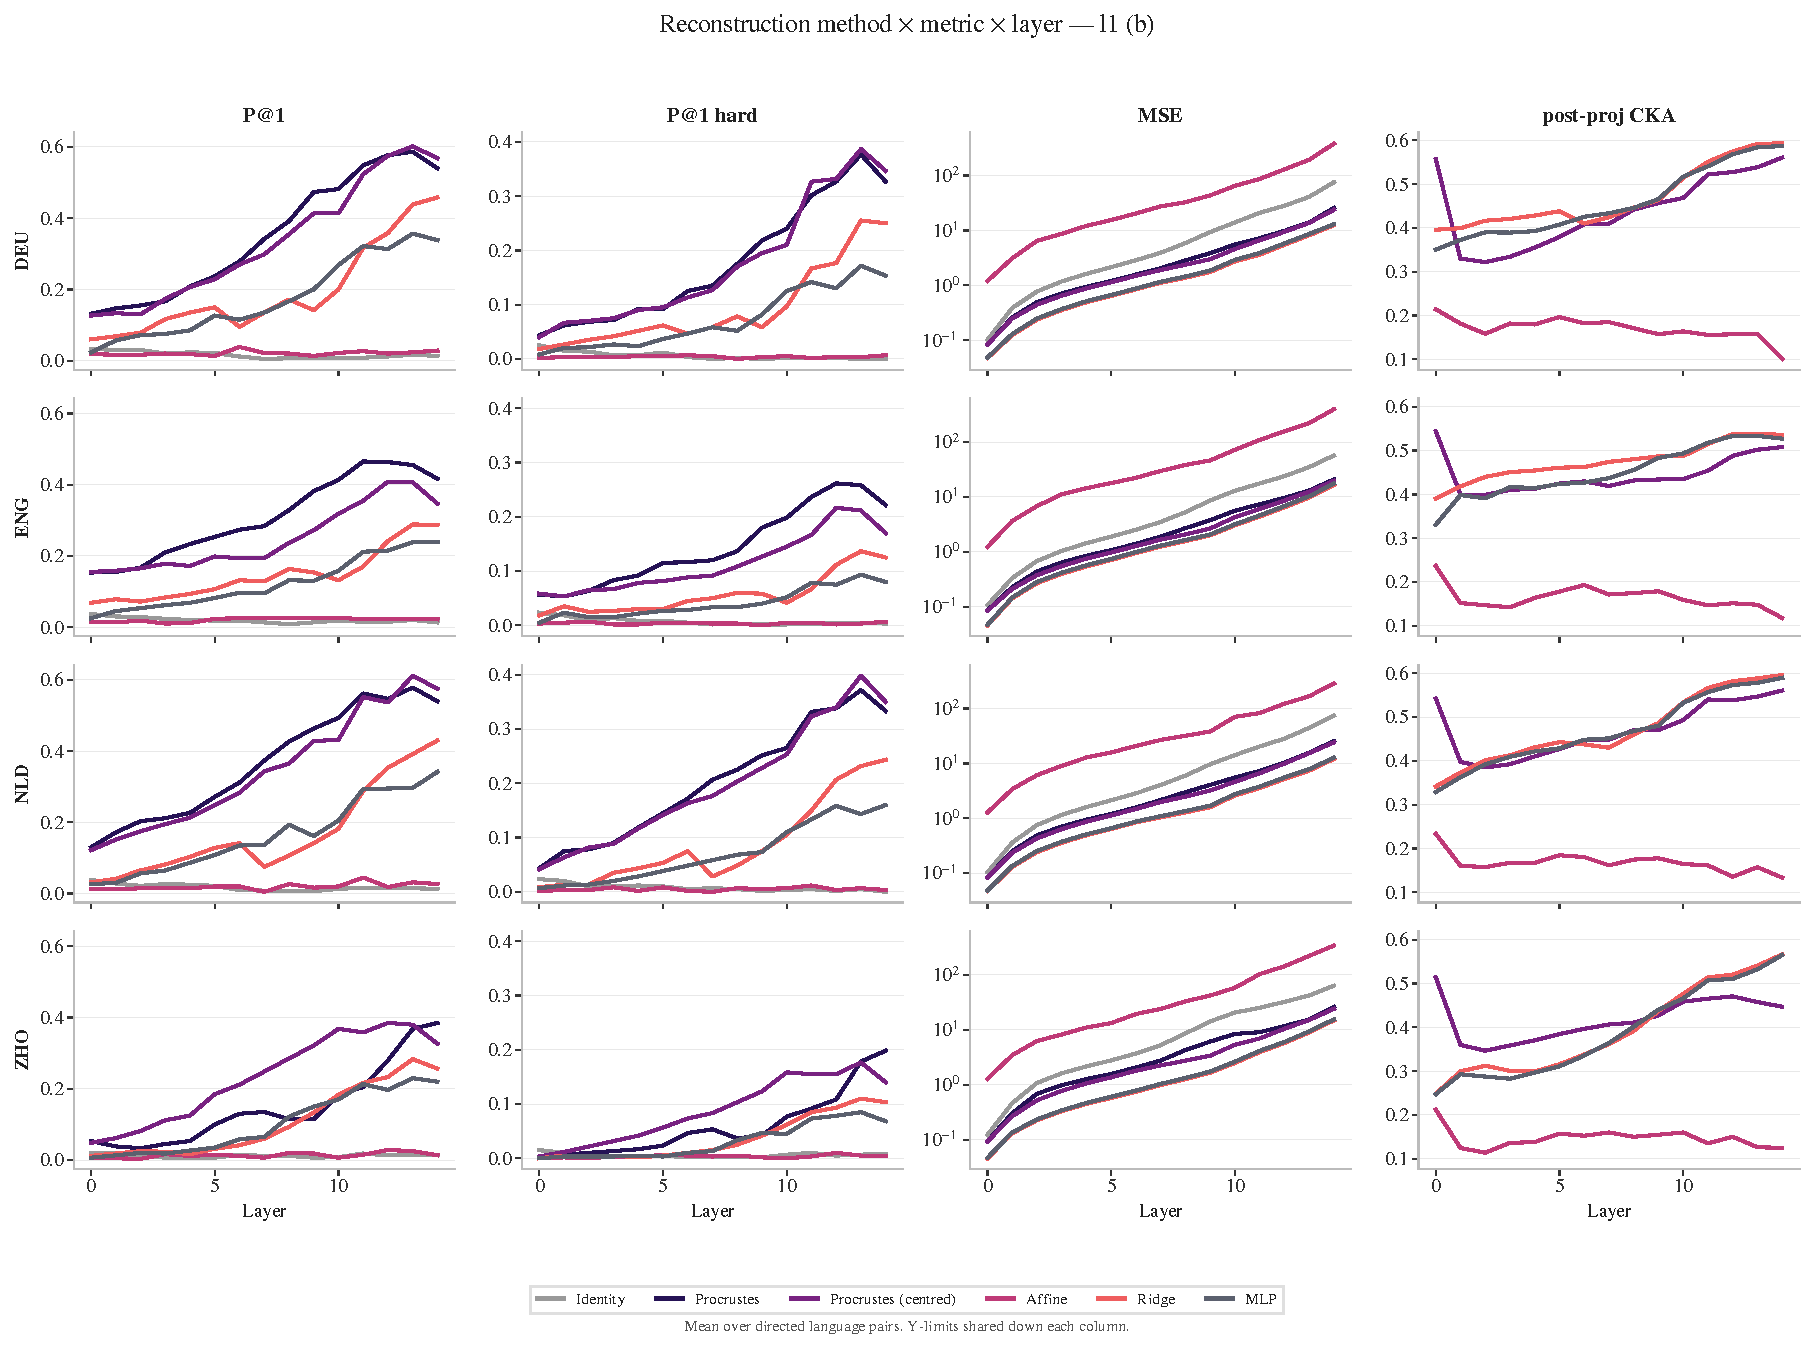
\includegraphics[width=\textwidth,height=0.74\textheight,keepaspectratio]{figures/fig10b_method_metric_layer_mono.pdf}
  \end{center}
  \vspace{-0.5em}\begin{center}\tiny {\tiny\texttt{\detokenize{fig10b_method_metric_layer_mono.pdf}}}\end{center}
\end{frame}

\begin{frame}{fig10: Method metric layer bilingual}
  \begin{center}
    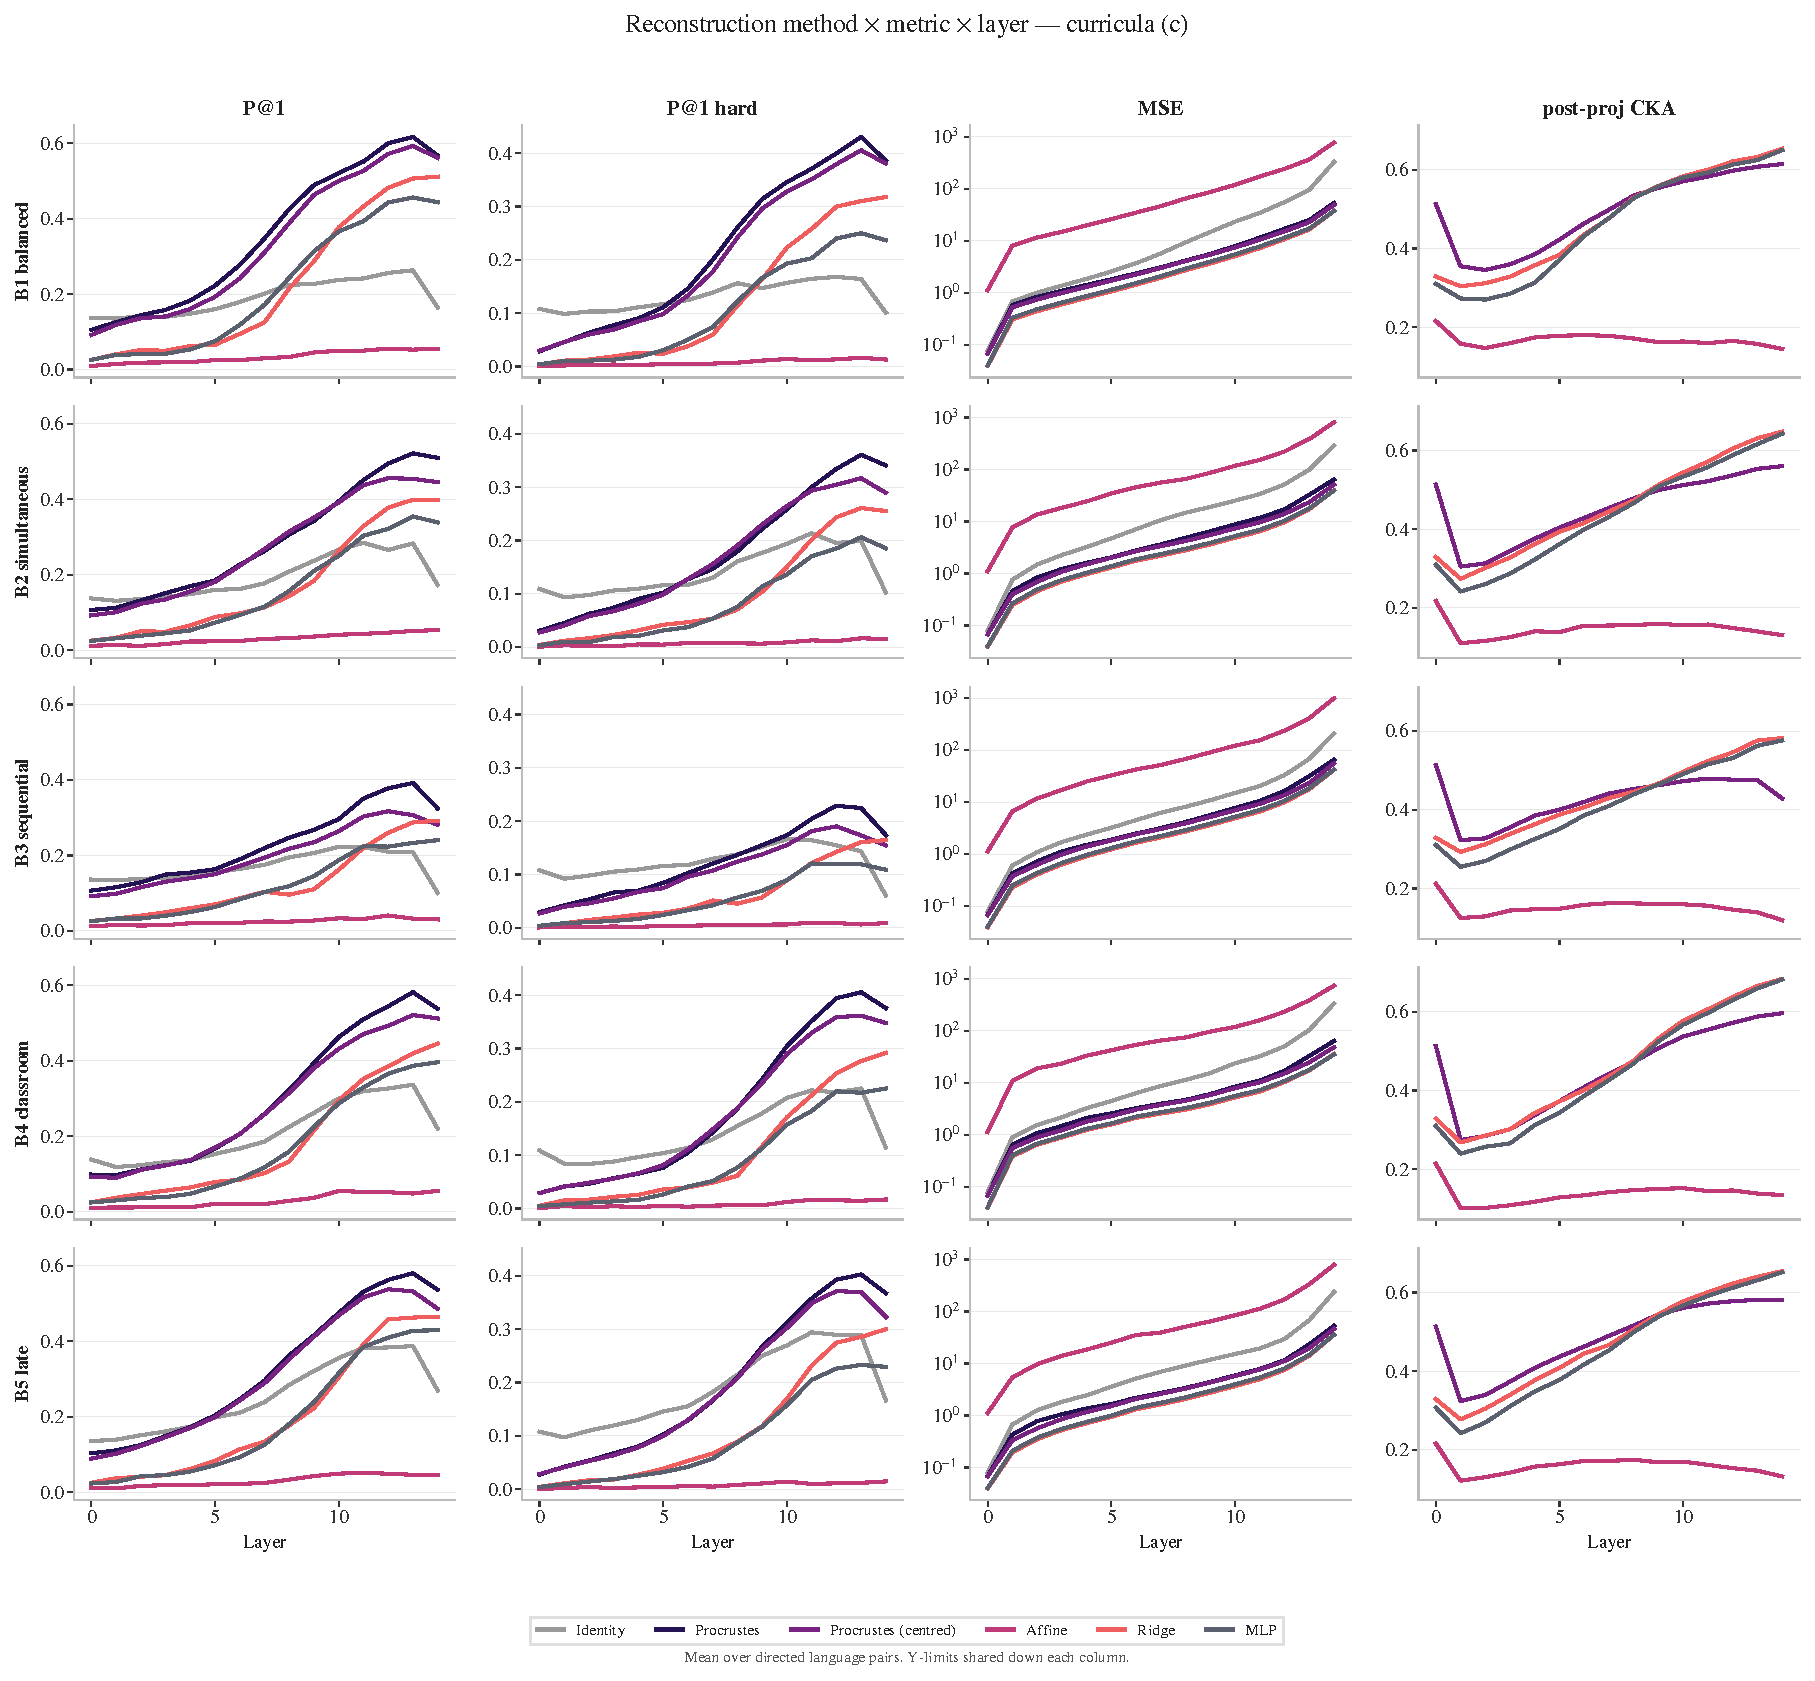
\includegraphics[width=\textwidth,height=0.74\textheight,keepaspectratio]{figures/fig10c_method_metric_layer_bilingual.pdf}
  \end{center}
  \vspace{-0.5em}\begin{center}\tiny {\tiny\texttt{\detokenize{fig10c_method_metric_layer_bilingual.pdf}}}\end{center}
\end{frame}

\begin{frame}{fig10: Method metric layer bilingual}
  \begin{center}
    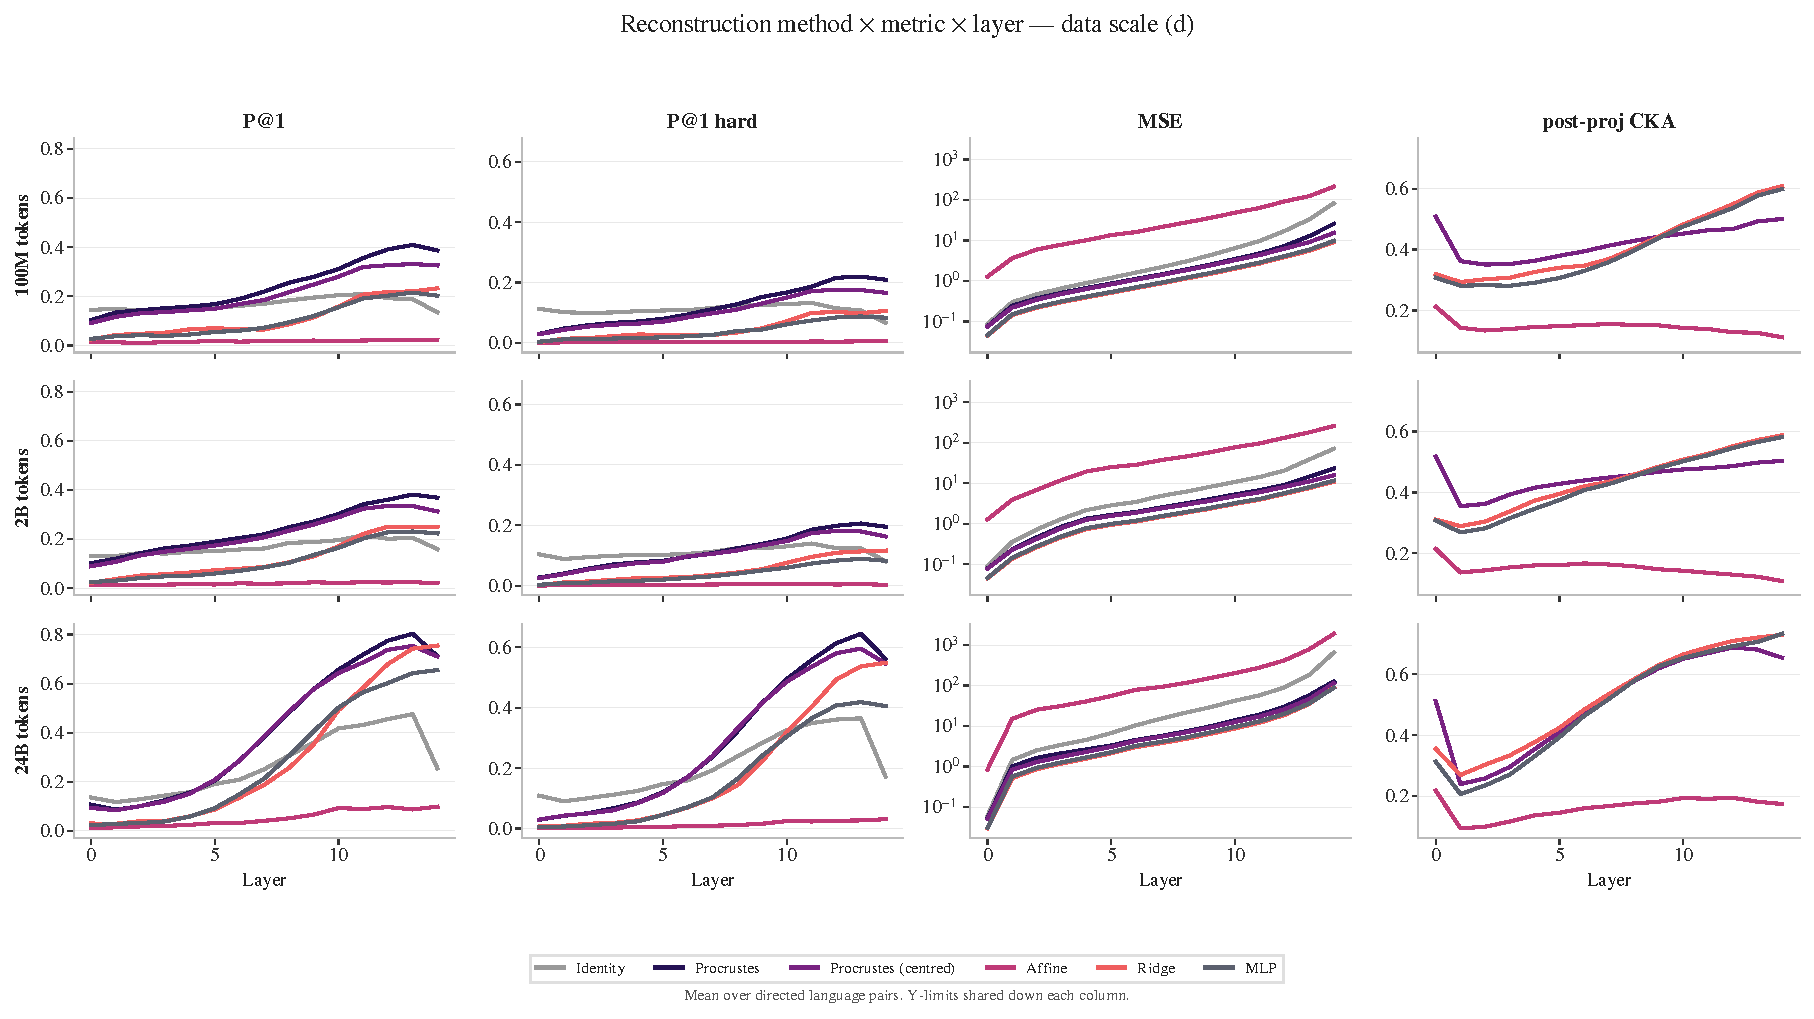
\includegraphics[width=\textwidth,height=0.74\textheight,keepaspectratio]{figures/fig10d_method_metric_layer_bilingual.pdf}
  \end{center}
  \vspace{-0.5em}\begin{center}\tiny {\tiny\texttt{\detokenize{fig10d_method_metric_layer_bilingual.pdf}}}\end{center}
\end{frame}

\subsection{Activation patching}

\begin{frame}{fig14: Patching}
  \begin{center}
    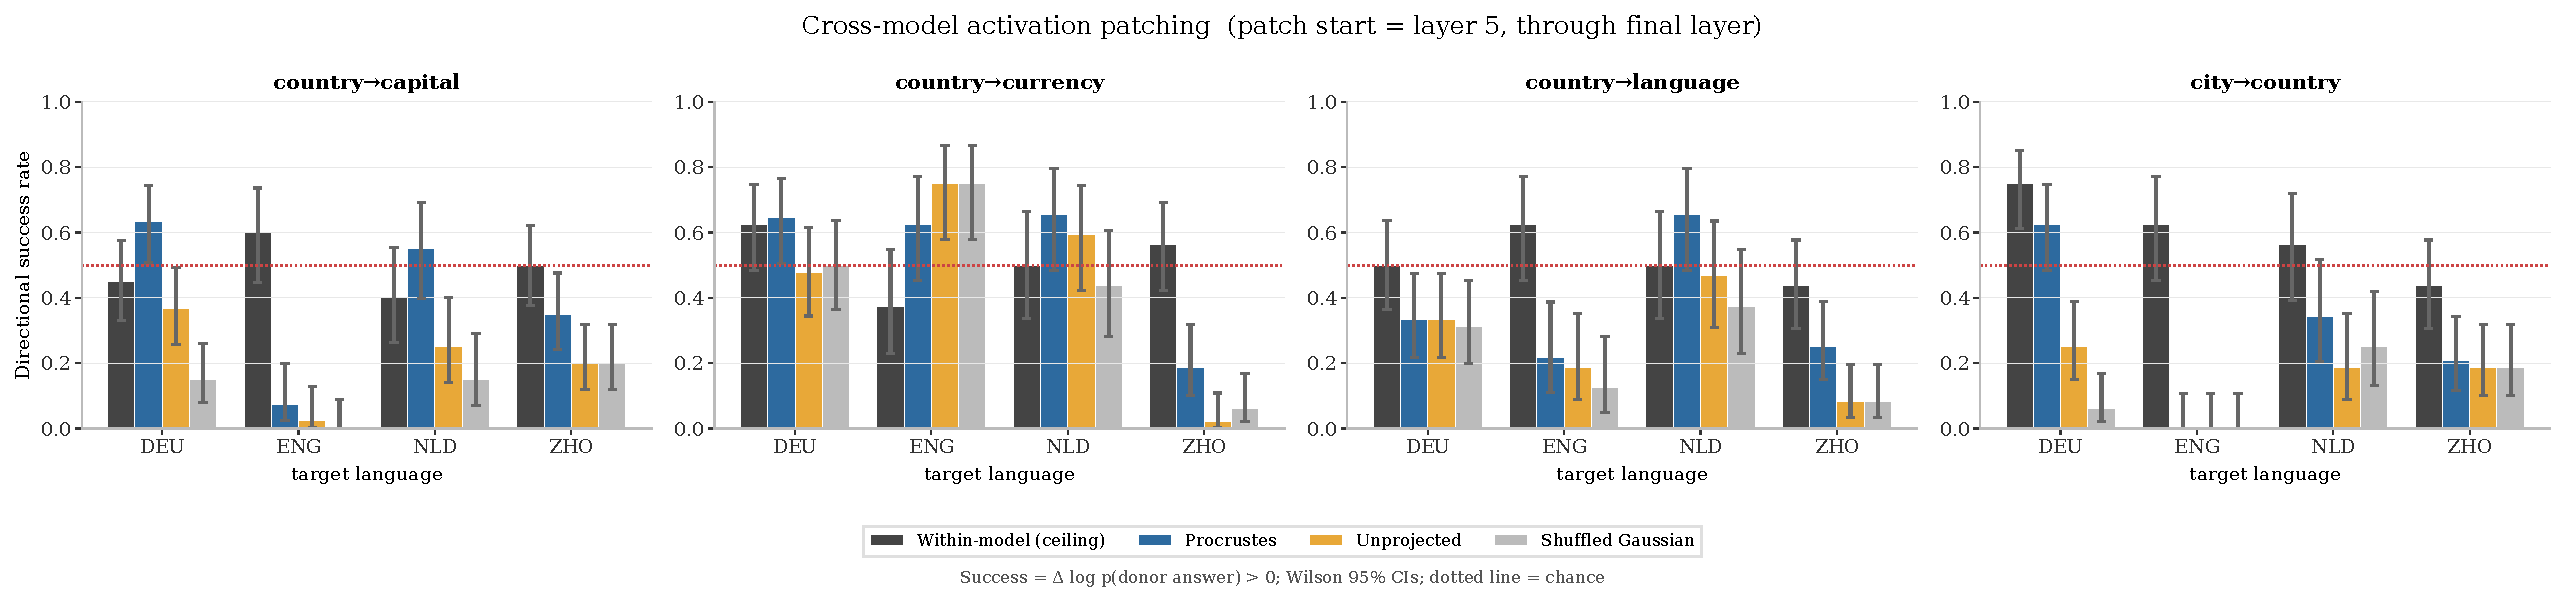
\includegraphics[width=\textwidth,height=0.74\textheight,keepaspectratio]{figures/fig14_patching.pdf}
  \end{center}
  \vspace{-0.5em}\begin{center}\tiny {\tiny\texttt{\detokenize{fig14_patching.pdf}}}\end{center}
\end{frame}

\subsection{Activation patching}

\begin{frame}{fig15: Patching}
  \begin{center}
    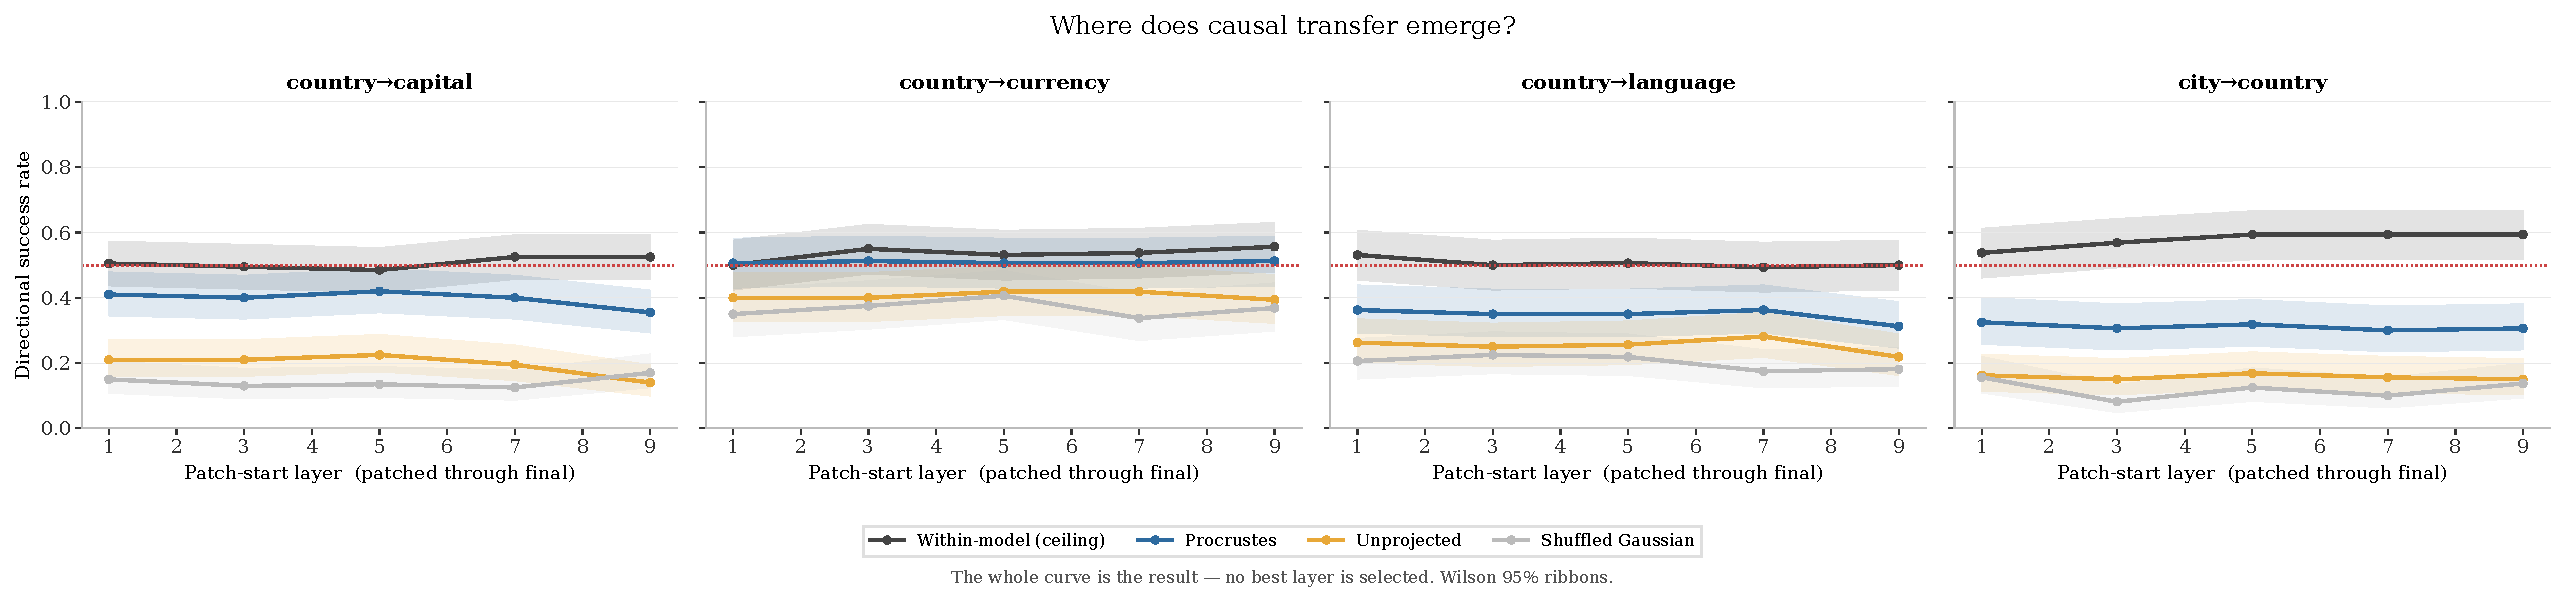
\includegraphics[width=\textwidth,height=0.74\textheight,keepaspectratio]{figures/fig15_patching.pdf}
  \end{center}
  \vspace{-0.5em}\begin{center}\tiny {\tiny\texttt{\detokenize{fig15_patching.pdf}}}\end{center}
\end{frame}

\subsection{Activation patching}

\begin{frame}{fig16: Patching}
  \begin{center}
    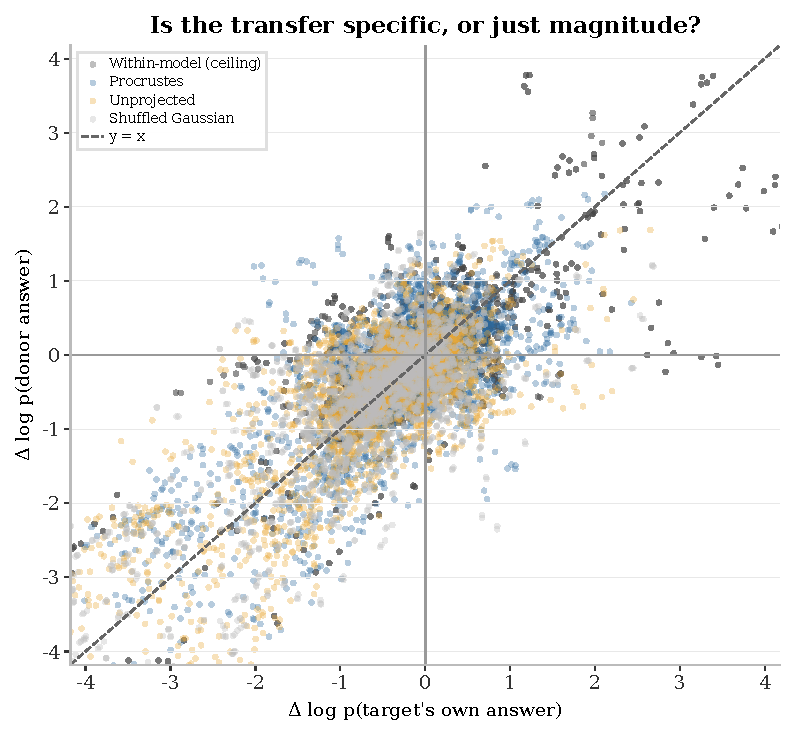
\includegraphics[width=\textwidth,height=0.74\textheight,keepaspectratio]{figures/fig16_patching.pdf}
  \end{center}
  \vspace{-0.5em}\begin{center}\tiny {\tiny\texttt{\detokenize{fig16_patching.pdf}}}\end{center}
\end{frame}

\subsection{Pooling robustness}

\begin{frame}{fig17: Pooling robustness FineWeb-100M}
  \begin{center}
    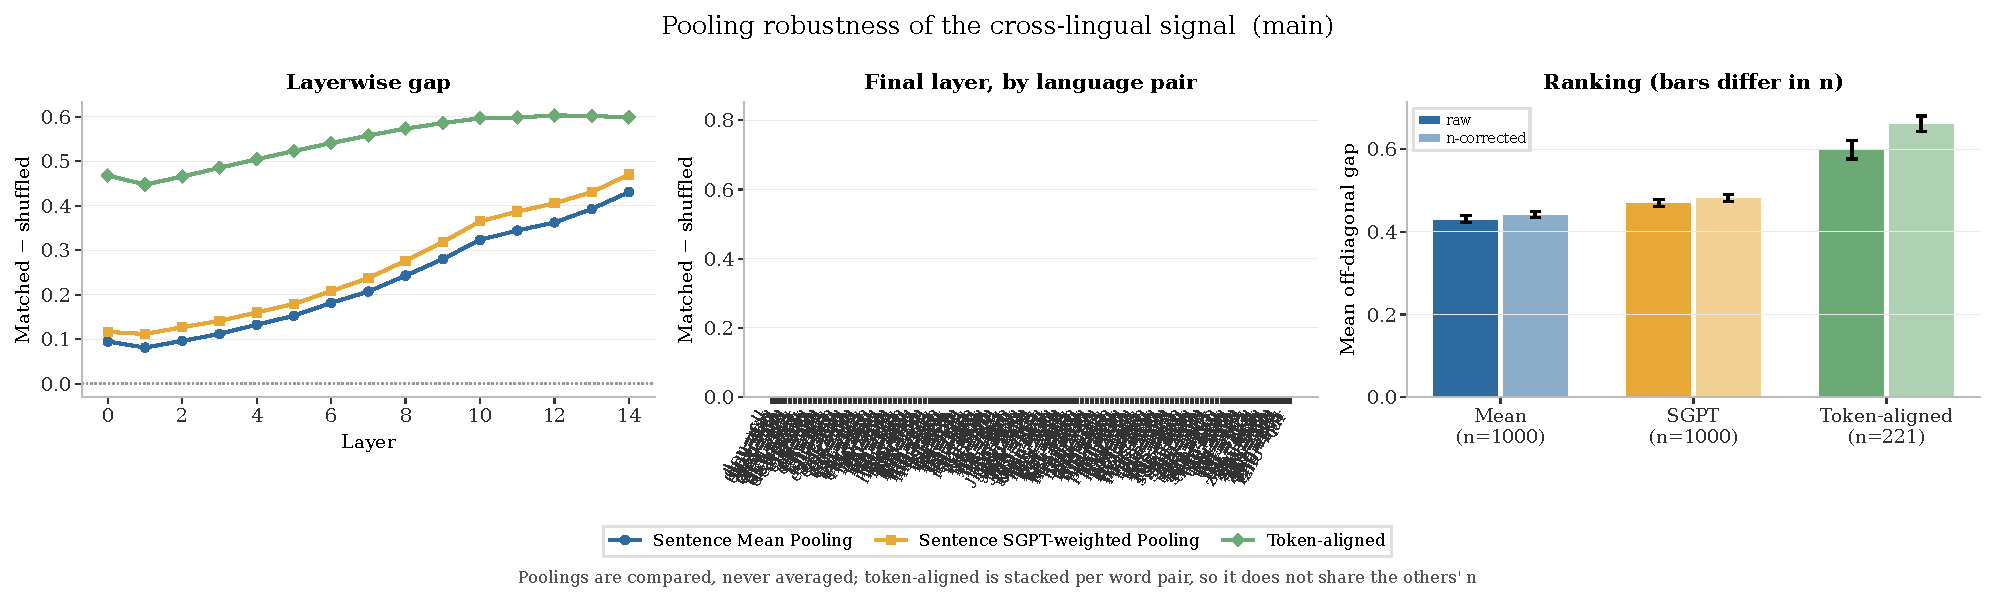
\includegraphics[width=\textwidth,height=0.74\textheight,keepaspectratio]{figures/fig17_pooling_robustness_fw100m.pdf}
  \end{center}
  \vspace{-0.5em}\begin{center}\tiny {\tiny\texttt{\detokenize{fig17_pooling_robustness_fw100m.pdf}}}\end{center}
\end{frame}

\begin{frame}{fig17: Pooling robustness main}
  \begin{center}
    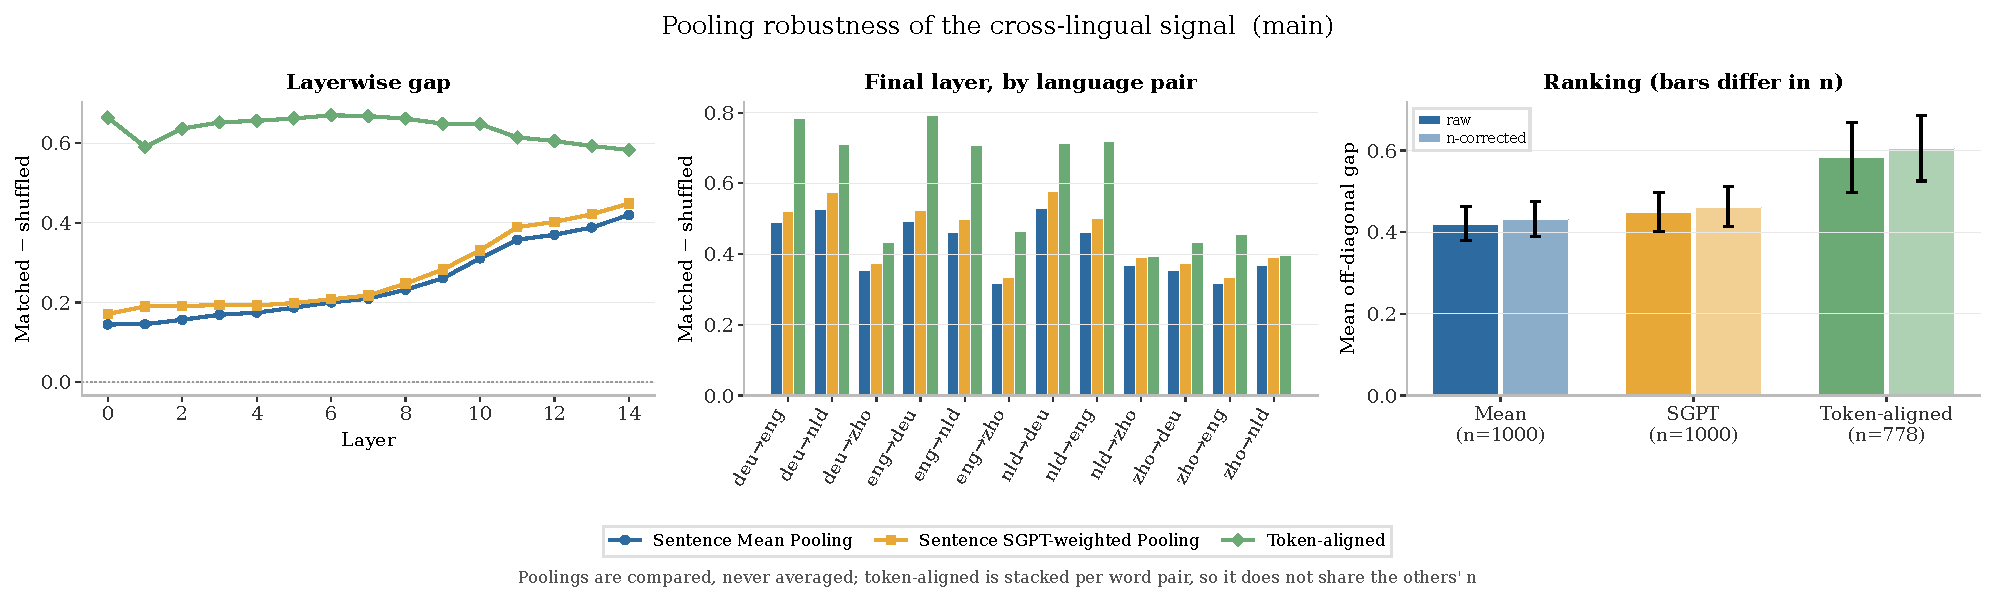
\includegraphics[width=\textwidth,height=0.74\textheight,keepaspectratio]{figures/fig17_pooling_robustness_main.pdf}
  \end{center}
  \vspace{-0.5em}\begin{center}\tiny {\tiny\texttt{\detokenize{fig17_pooling_robustness_main.pdf}}}\end{center}
\end{frame}

\subsection{Quantity and condition}

\begin{frame}{fig18: Quantity condition SGPT pooling delta}
  \begin{center}
    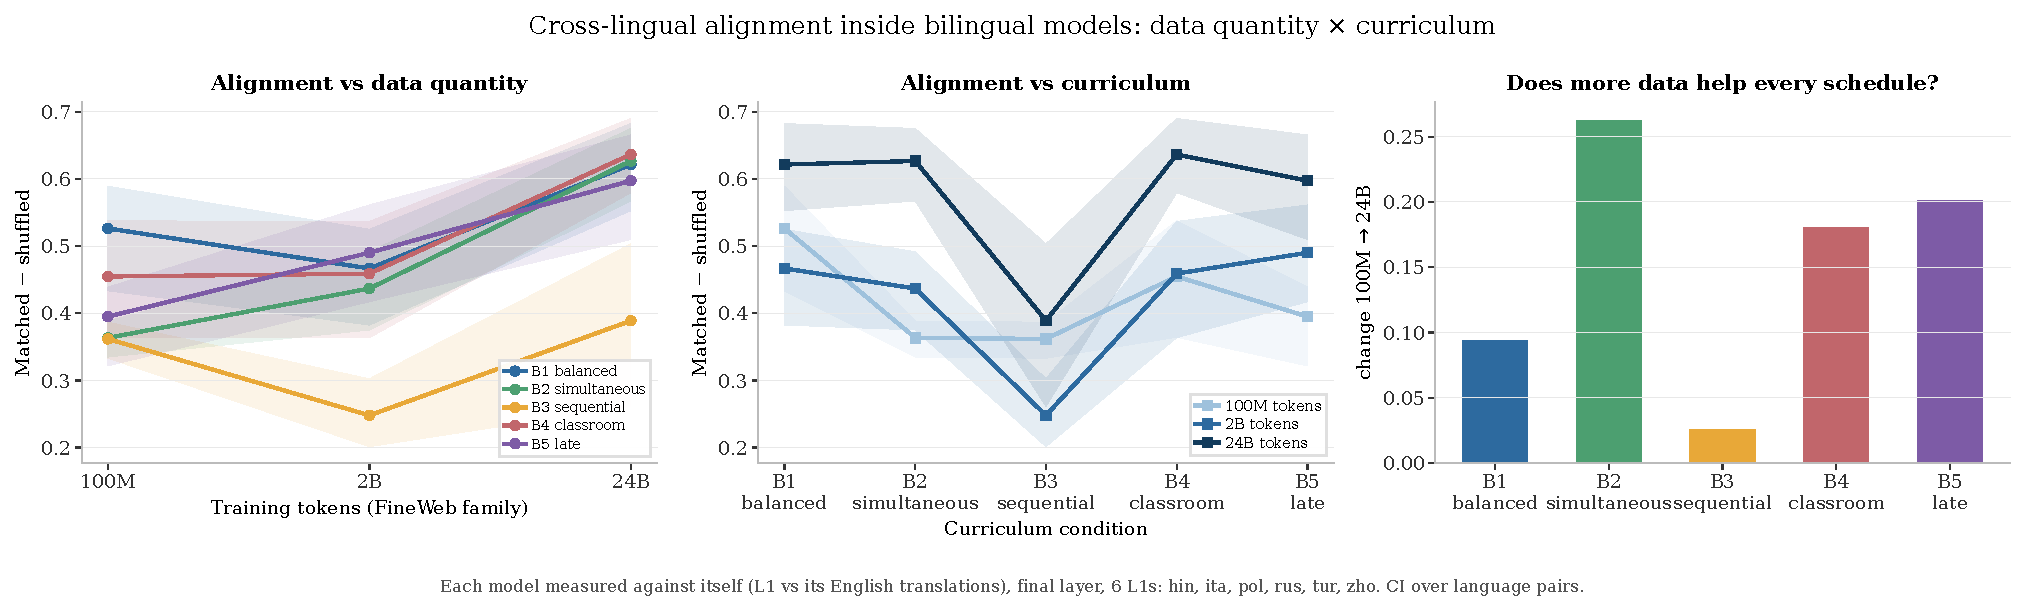
\includegraphics[width=\textwidth,height=0.74\textheight,keepaspectratio]{figures/fig18_quantity_condition_sgpt_delta.pdf}
  \end{center}
  \vspace{-0.5em}\begin{center}\tiny {\tiny\texttt{\detokenize{fig18_quantity_condition_sgpt_delta.pdf}}}\end{center}
\end{frame}

\subsection{Three effects}

\begin{frame}{fig19: Three effects SGPT pooling}
  \begin{center}
    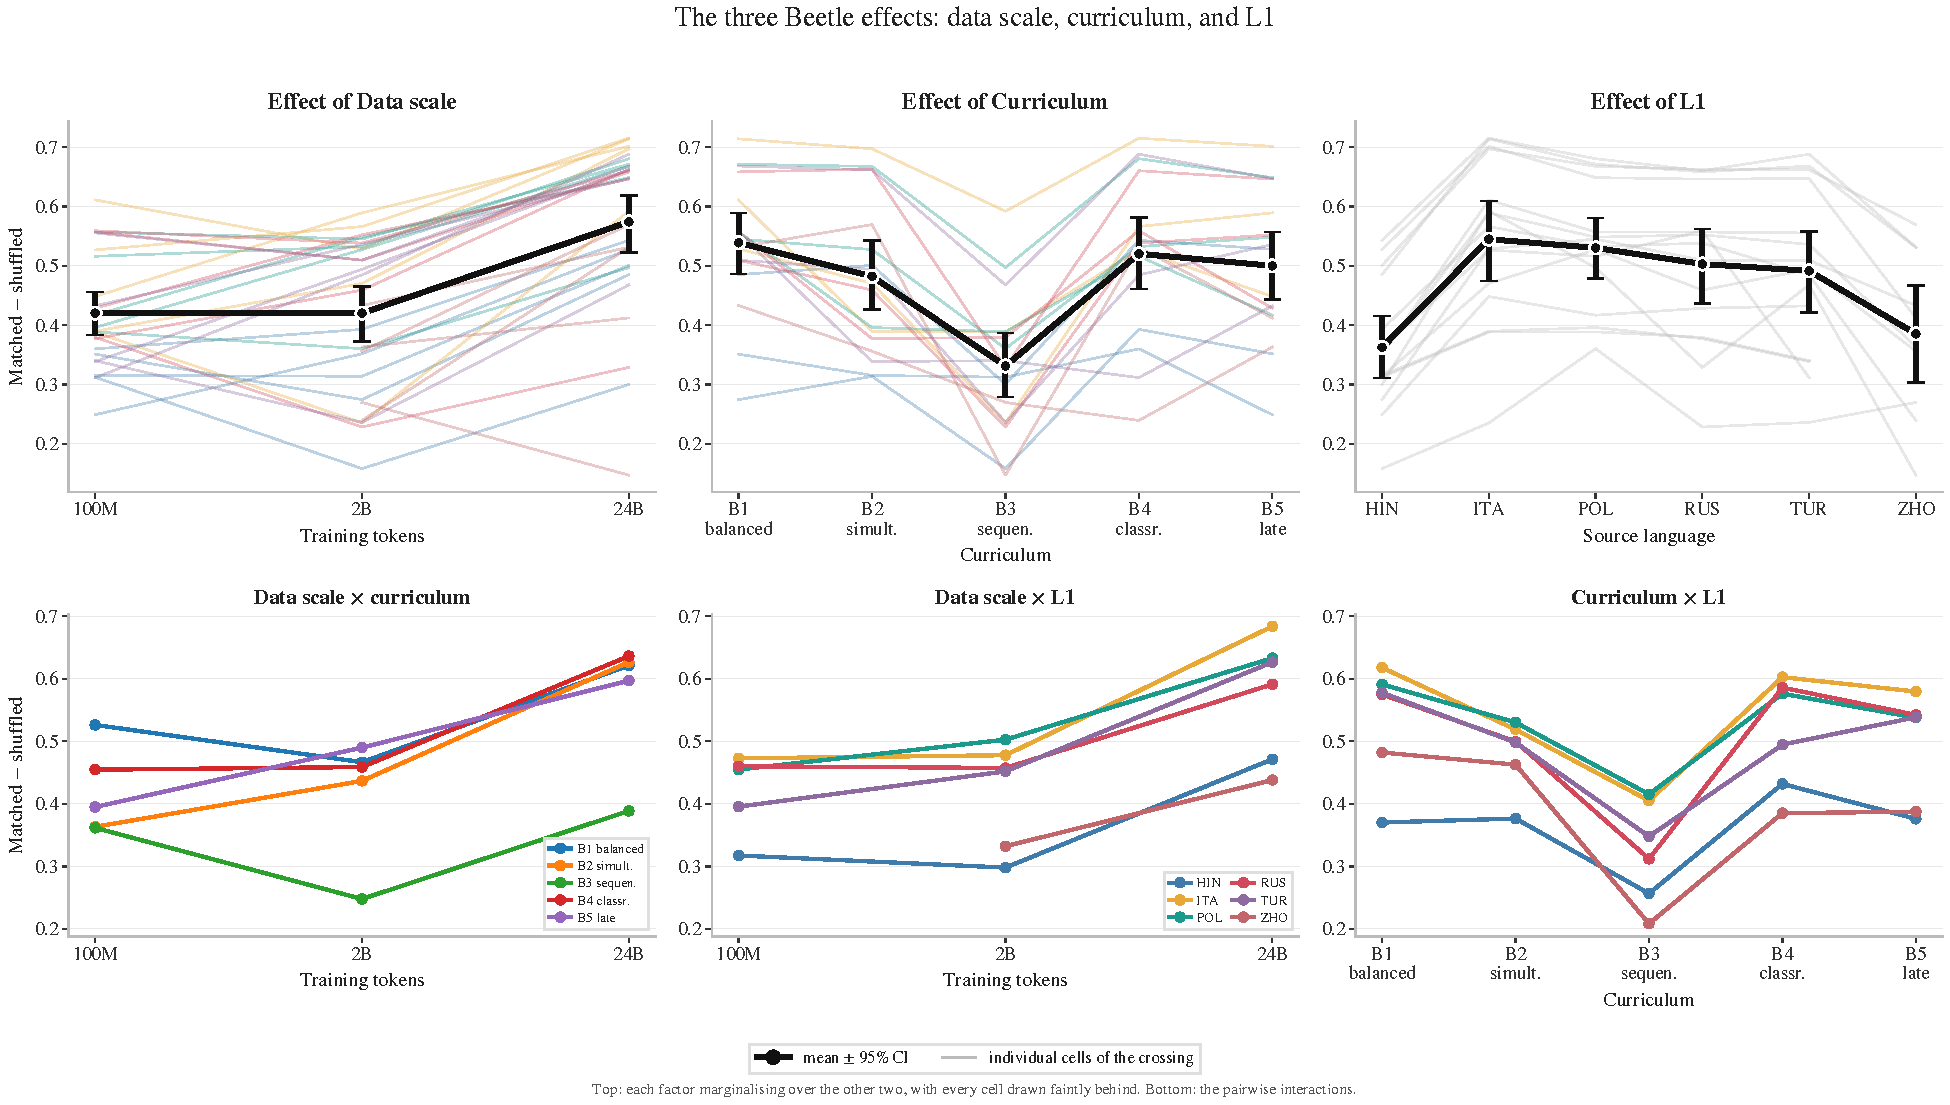
\includegraphics[width=\textwidth,height=0.74\textheight,keepaspectratio]{figures/fig19_three_effects_sgpt.pdf}
  \end{center}
  \vspace{-0.5em}\begin{center}\tiny {\tiny\texttt{\detokenize{fig19_three_effects_sgpt.pdf}}}\end{center}
\end{frame}

\subsection{Layer-wise profiles by condition}

\begin{frame}{gfE2: Layerwise bilingual}
  \begin{center}
    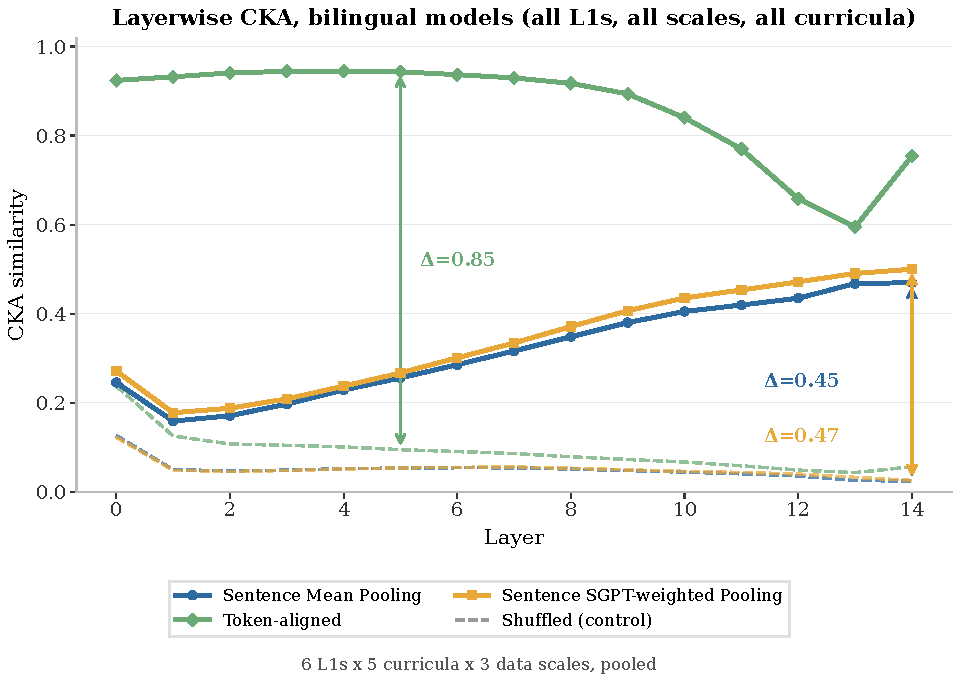
\includegraphics[width=\textwidth,height=0.74\textheight,keepaspectratio]{figures/gfE2_layerwise_bilingual.pdf}
  \end{center}
  \vspace{-0.5em}\begin{center}\tiny {\tiny\texttt{\detokenize{gfE2_layerwise_bilingual.pdf}}}\end{center}
\end{frame}

\begin{frame}{gfE2: Layerwise curr b1}
  \begin{center}
    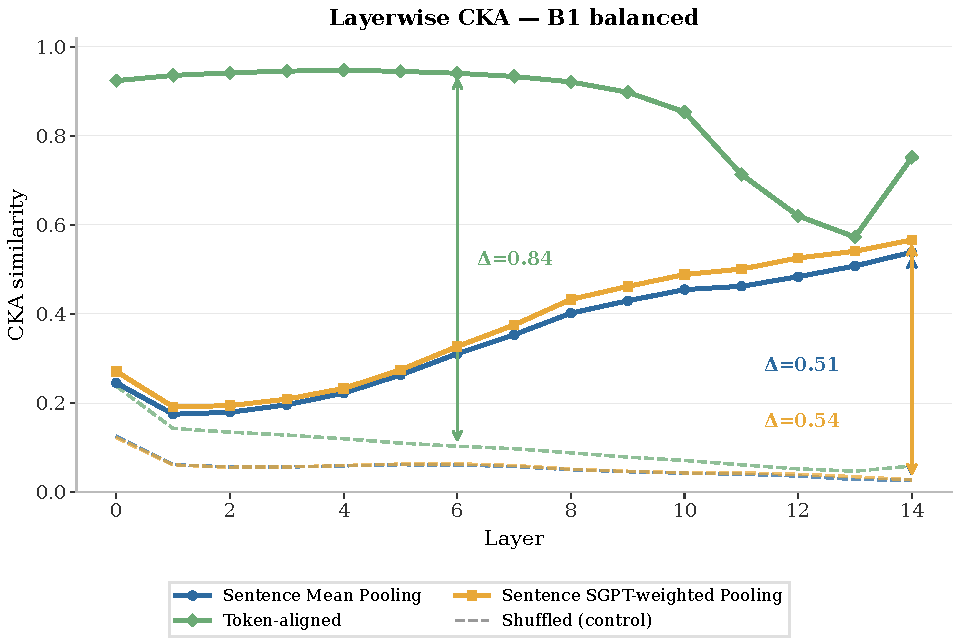
\includegraphics[width=\textwidth,height=0.74\textheight,keepaspectratio]{figures/gfE2_layerwise_curr_b1.pdf}
  \end{center}
  \vspace{-0.5em}\begin{center}\tiny {\tiny\texttt{\detokenize{gfE2_layerwise_curr_b1.pdf}}}\end{center}
\end{frame}

\begin{frame}{gfE2: Layerwise curr b2}
  \begin{center}
    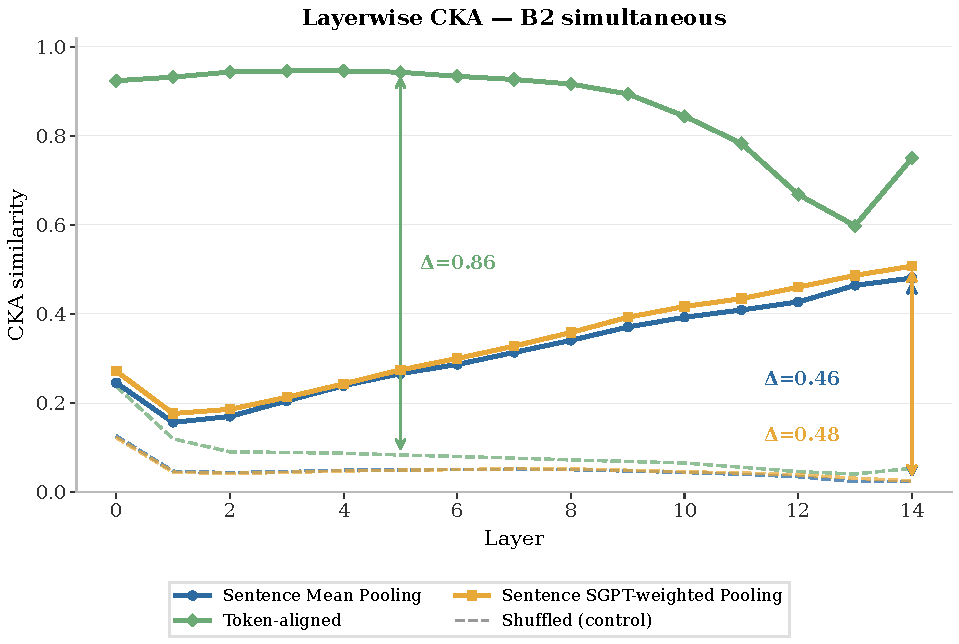
\includegraphics[width=\textwidth,height=0.74\textheight,keepaspectratio]{figures/gfE2_layerwise_curr_b2.pdf}
  \end{center}
  \vspace{-0.5em}\begin{center}\tiny {\tiny\texttt{\detokenize{gfE2_layerwise_curr_b2.pdf}}}\end{center}
\end{frame}

\begin{frame}{gfE2: Layerwise curr b3}
  \begin{center}
    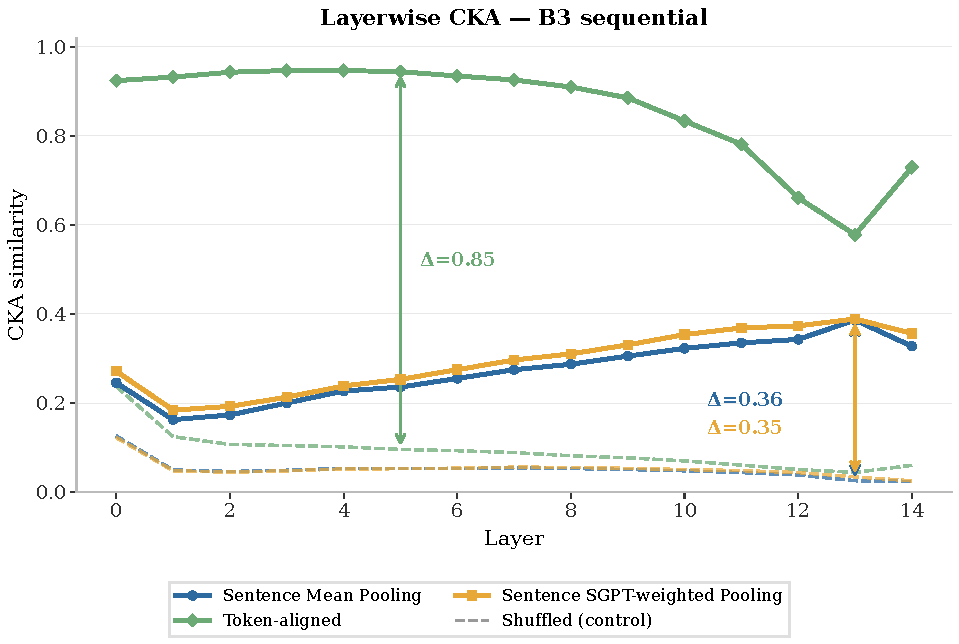
\includegraphics[width=\textwidth,height=0.74\textheight,keepaspectratio]{figures/gfE2_layerwise_curr_b3.pdf}
  \end{center}
  \vspace{-0.5em}\begin{center}\tiny {\tiny\texttt{\detokenize{gfE2_layerwise_curr_b3.pdf}}}\end{center}
\end{frame}

\begin{frame}{gfE2: Layerwise curr b4}
  \begin{center}
    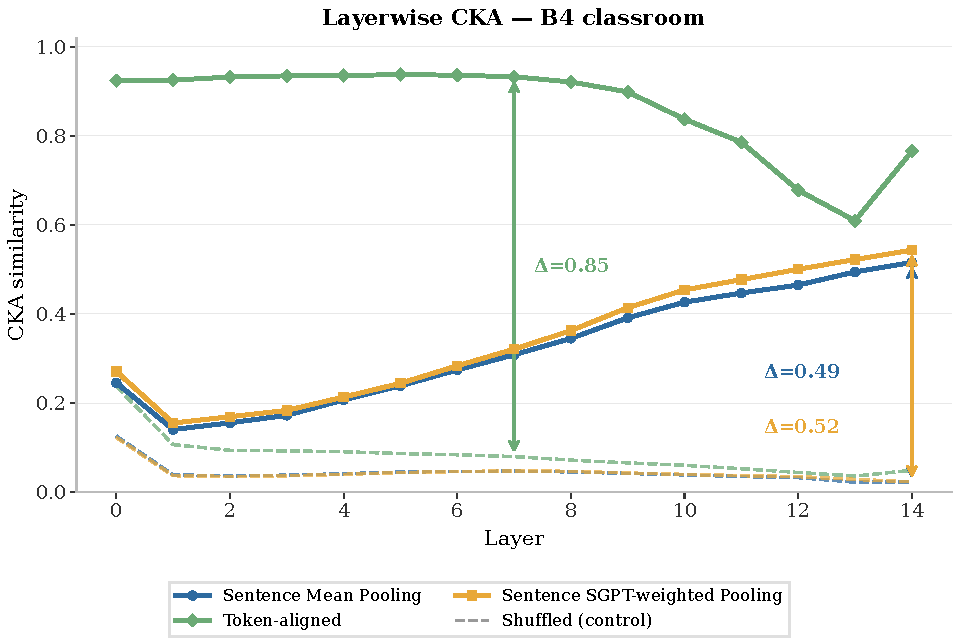
\includegraphics[width=\textwidth,height=0.74\textheight,keepaspectratio]{figures/gfE2_layerwise_curr_b4.pdf}
  \end{center}
  \vspace{-0.5em}\begin{center}\tiny {\tiny\texttt{\detokenize{gfE2_layerwise_curr_b4.pdf}}}\end{center}
\end{frame}

\begin{frame}{gfE2: Layerwise curr b5}
  \begin{center}
    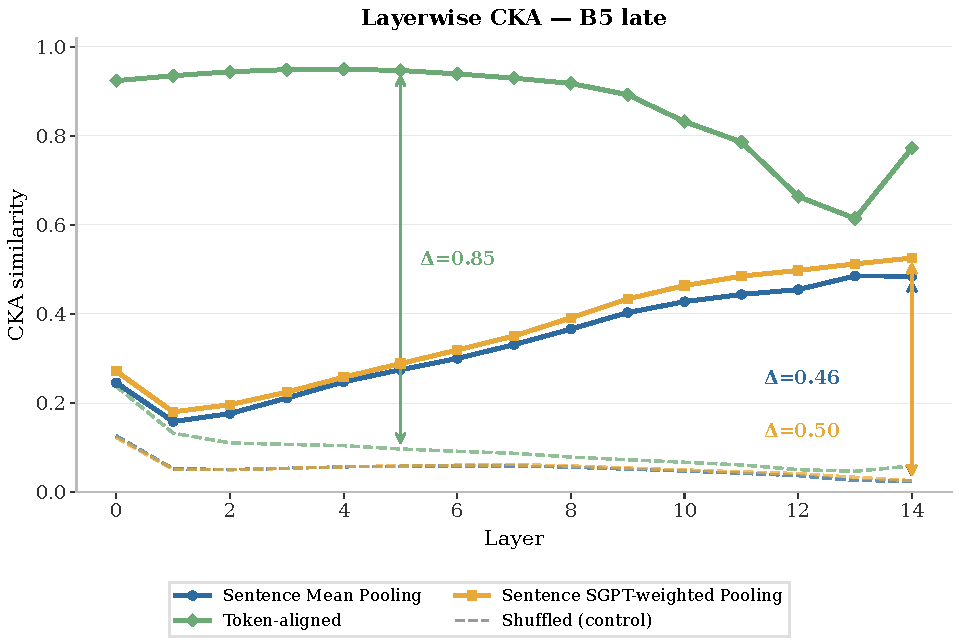
\includegraphics[width=\textwidth,height=0.74\textheight,keepaspectratio]{figures/gfE2_layerwise_curr_b5.pdf}
  \end{center}
  \vspace{-0.5em}\begin{center}\tiny {\tiny\texttt{\detokenize{gfE2_layerwise_curr_b5.pdf}}}\end{center}
\end{frame}

\begin{frame}{gfE2: Layerwise scale 100M}
  \begin{center}
    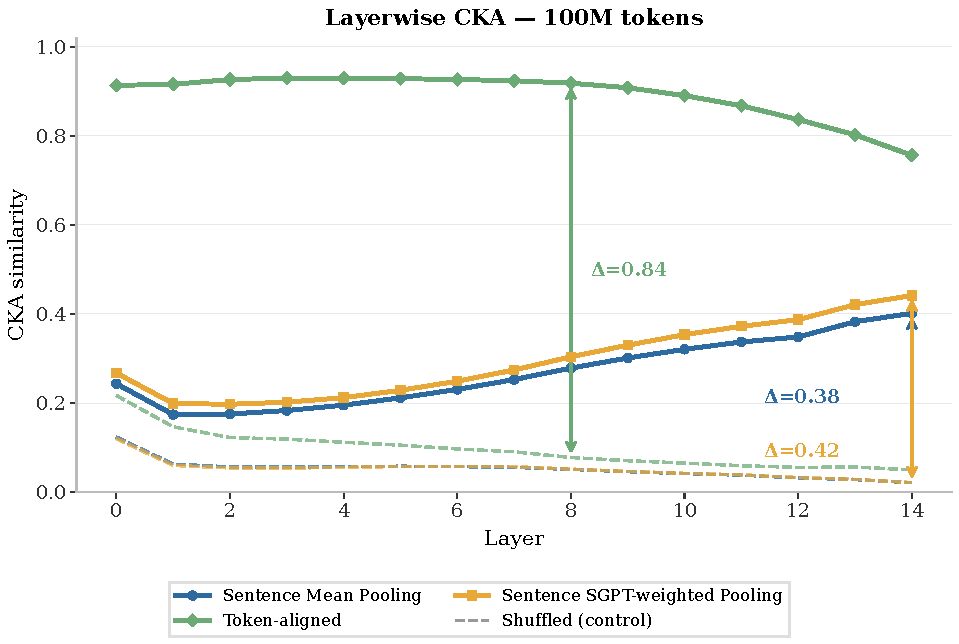
\includegraphics[width=\textwidth,height=0.74\textheight,keepaspectratio]{figures/gfE2_layerwise_scale_100M.pdf}
  \end{center}
  \vspace{-0.5em}\begin{center}\tiny {\tiny\texttt{\detokenize{gfE2_layerwise_scale_100M.pdf}}}\end{center}
\end{frame}

\begin{frame}{gfE2: Layerwise scale 24B}
  \begin{center}
    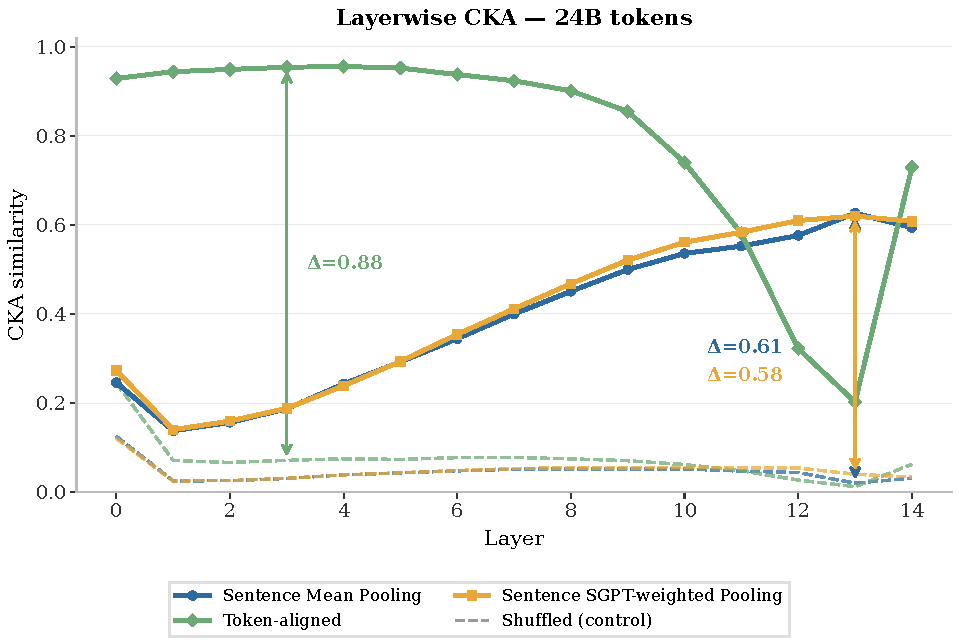
\includegraphics[width=\textwidth,height=0.74\textheight,keepaspectratio]{figures/gfE2_layerwise_scale_24B.pdf}
  \end{center}
  \vspace{-0.5em}\begin{center}\tiny {\tiny\texttt{\detokenize{gfE2_layerwise_scale_24B.pdf}}}\end{center}
\end{frame}

\begin{frame}{gfE2: Layerwise scale 2B}
  \begin{center}
    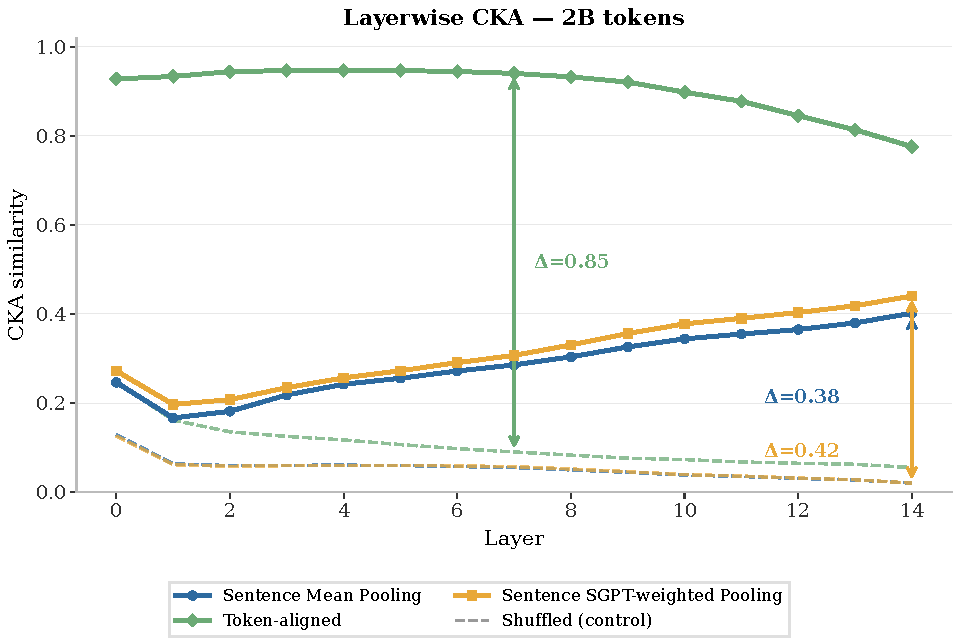
\includegraphics[width=\textwidth,height=0.74\textheight,keepaspectratio]{figures/gfE2_layerwise_scale_2B.pdf}
  \end{center}
  \vspace{-0.5em}\begin{center}\tiny {\tiny\texttt{\detokenize{gfE2_layerwise_scale_2B.pdf}}}\end{center}
\end{frame}

\subsection{Triangular similarity, monolingual}

\begin{frame}{gfE3: Triangular mono FineWeb-100M}
  \begin{center}
    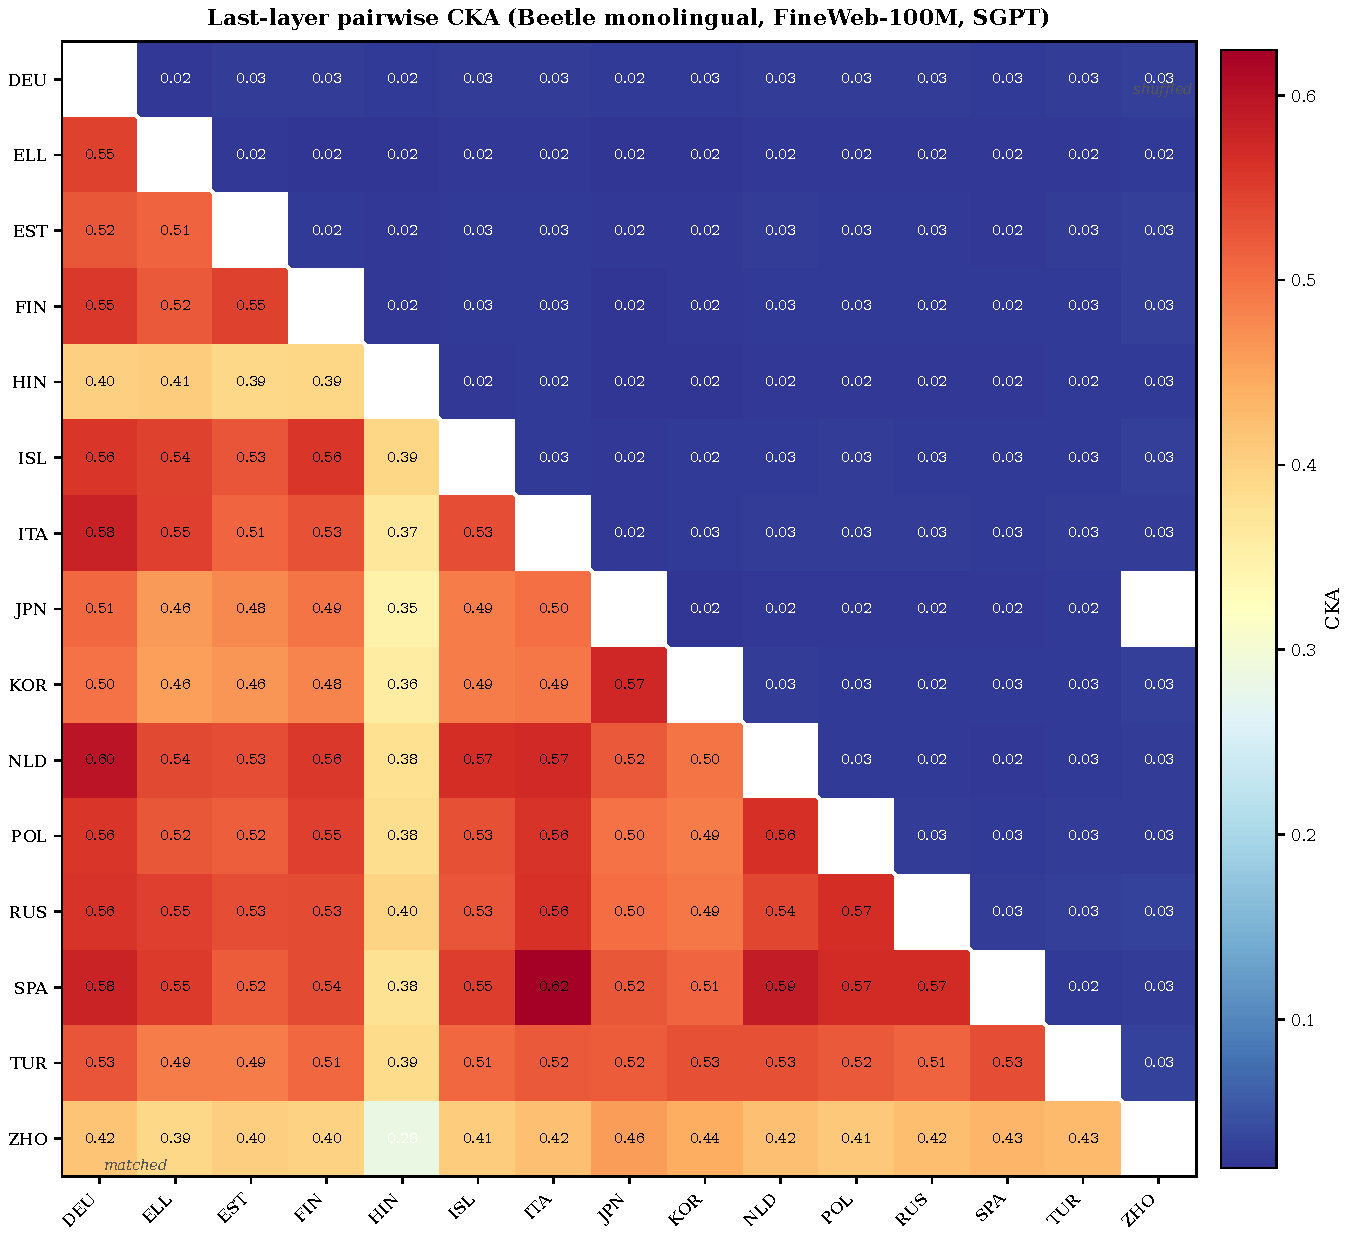
\includegraphics[width=\textwidth,height=0.74\textheight,keepaspectratio]{figures/gfE3_triangular_mono_fw100m.pdf}
  \end{center}
  \vspace{-0.5em}\begin{center}\tiny {\tiny\texttt{\detokenize{gfE3_triangular_mono_fw100m.pdf}}}\end{center}
\end{frame}

\subsection{Scaling}

\begin{frame}{gfE4: Scaling curriculum}
  \begin{center}
    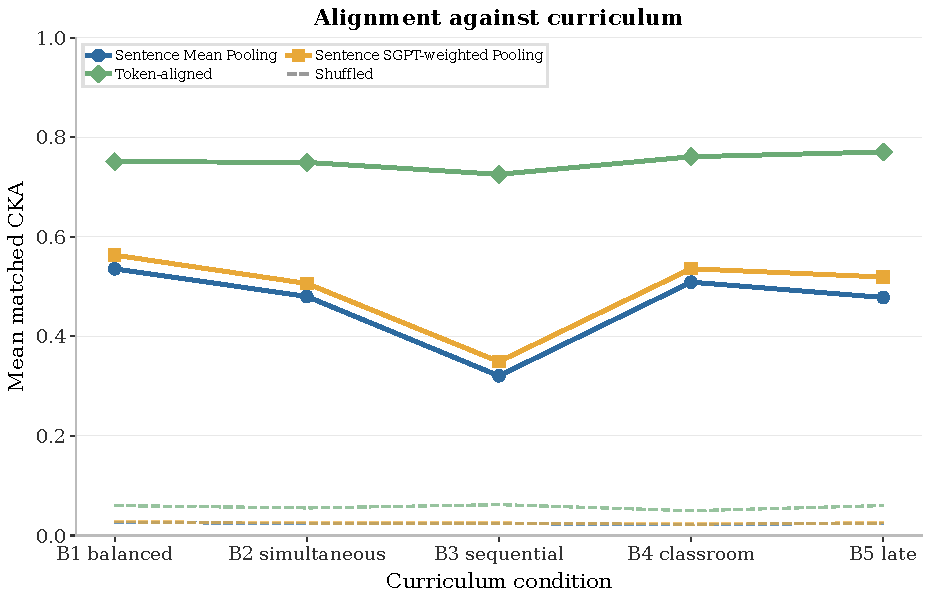
\includegraphics[width=\textwidth,height=0.74\textheight,keepaspectratio]{figures/gfE4_scaling_curriculum.pdf}
  \end{center}
  \vspace{-0.5em}\begin{center}\tiny {\tiny\texttt{\detokenize{gfE4_scaling_curriculum.pdf}}}\end{center}
\end{frame}

\begin{frame}{gfE4: Scaling quantity}
  \begin{center}
    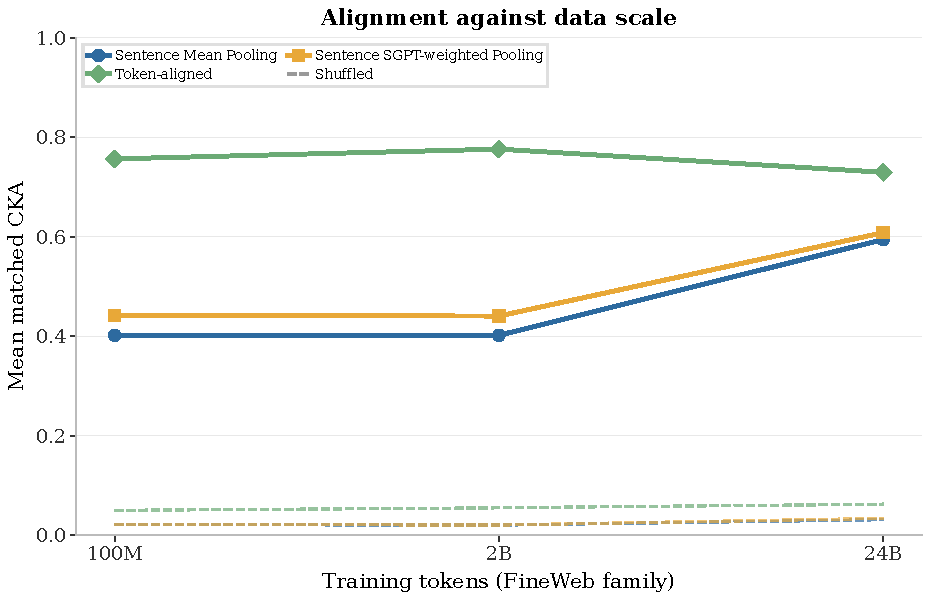
\includegraphics[width=\textwidth,height=0.74\textheight,keepaspectratio]{figures/gfE4_scaling_quantity.pdf}
  \end{center}
  \vspace{-0.5em}\begin{center}\tiny {\tiny\texttt{\detokenize{gfE4_scaling_quantity.pdf}}}\end{center}
\end{frame}

\subsection{PCA of representations}

\begin{frame}{gfE5: PCA eng deu}
  \begin{center}
    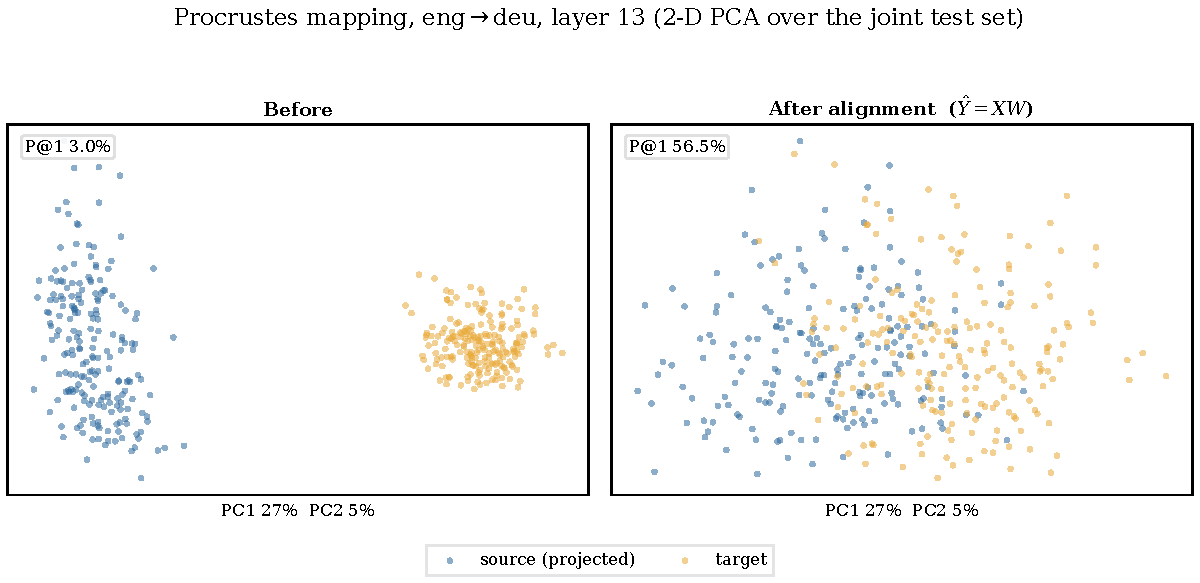
\includegraphics[width=\textwidth,height=0.74\textheight,keepaspectratio]{figures/gfE5_pca_eng_deu.pdf}
  \end{center}
  \vspace{-0.5em}\begin{center}\tiny {\tiny\texttt{\detokenize{gfE5_pca_eng_deu.pdf}}}\end{center}
\end{frame}

\begin{frame}{gfE5: PCA eng nld}
  \begin{center}
    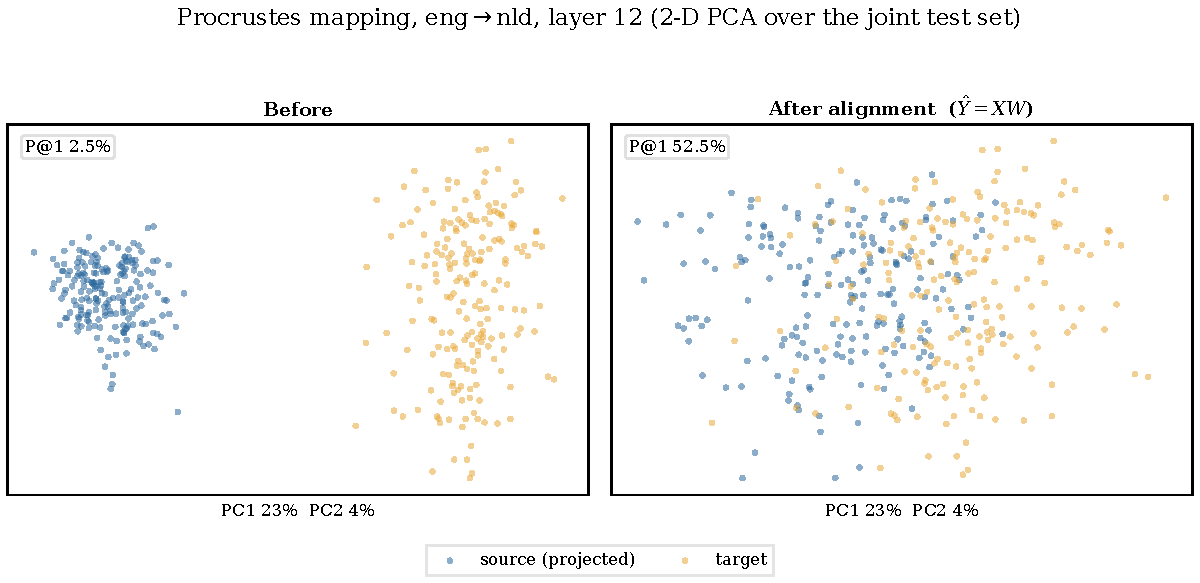
\includegraphics[width=\textwidth,height=0.74\textheight,keepaspectratio]{figures/gfE5_pca_eng_nld.pdf}
  \end{center}
  \vspace{-0.5em}\begin{center}\tiny {\tiny\texttt{\detokenize{gfE5_pca_eng_nld.pdf}}}\end{center}
\end{frame}

\begin{frame}{gfE5: PCA eng zho}
  \begin{center}
    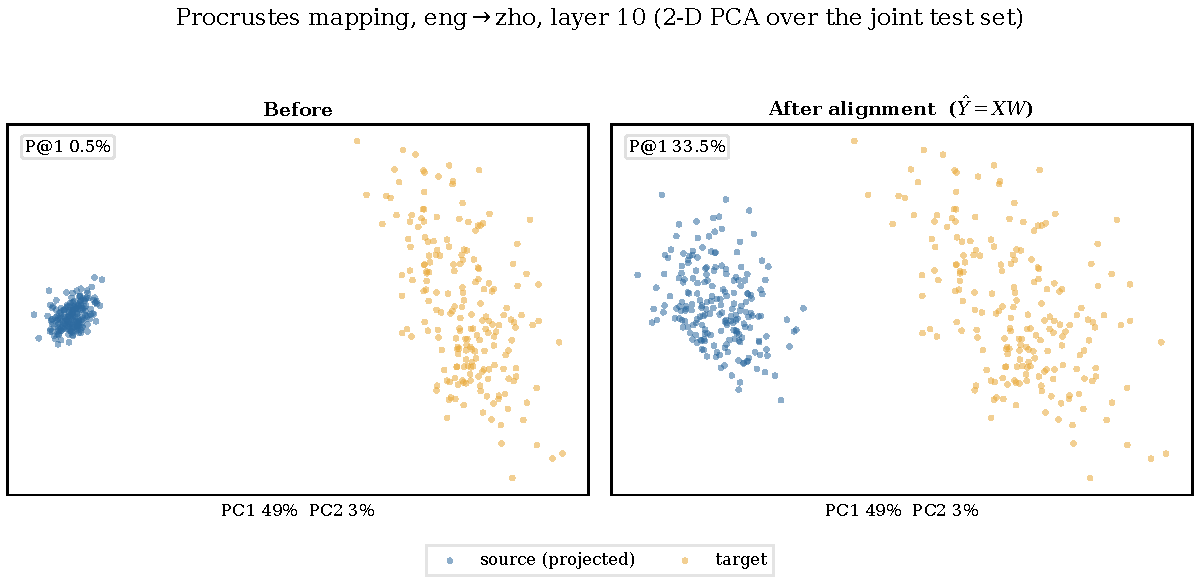
\includegraphics[width=\textwidth,height=0.74\textheight,keepaspectratio]{figures/gfE5_pca_eng_zho.pdf}
  \end{center}
  \vspace{-0.5em}\begin{center}\tiny {\tiny\texttt{\detokenize{gfE5_pca_eng_zho.pdf}}}\end{center}
\end{frame}

\begin{frame}{gfE5: PCA nld deu}
  \begin{center}
    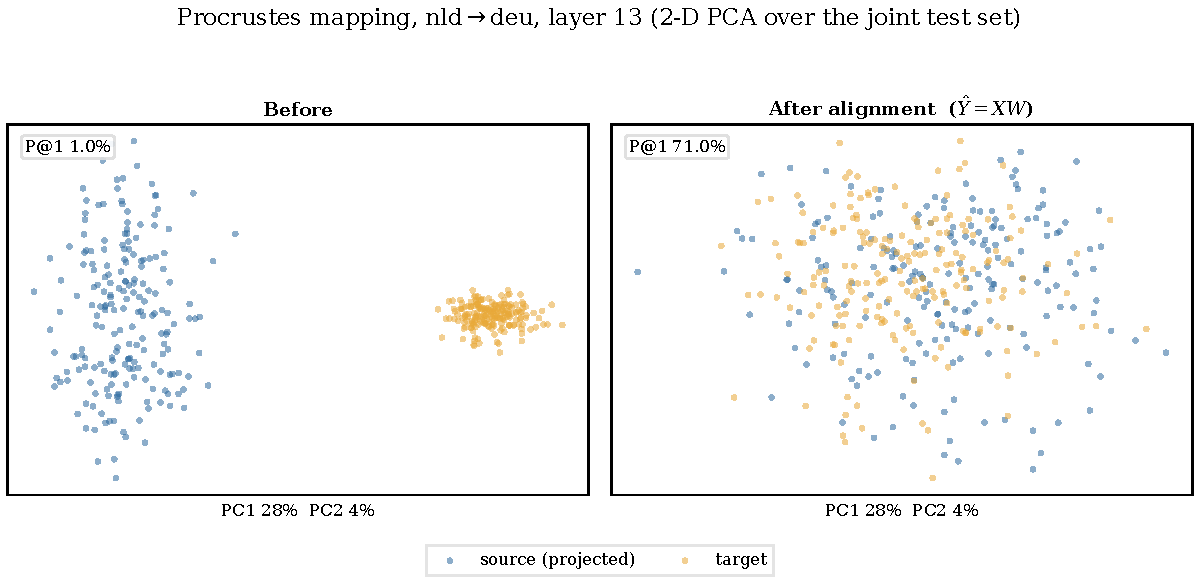
\includegraphics[width=\textwidth,height=0.74\textheight,keepaspectratio]{figures/gfE5_pca_nld_deu.pdf}
  \end{center}
  \vspace{-0.5em}\begin{center}\tiny {\tiny\texttt{\detokenize{gfE5_pca_nld_deu.pdf}}}\end{center}
\end{frame}

\subsection{Beetle vs Goldfish}

\begin{frame}{gfE10: Beetle vs goldfish mean pool}
  \begin{center}
    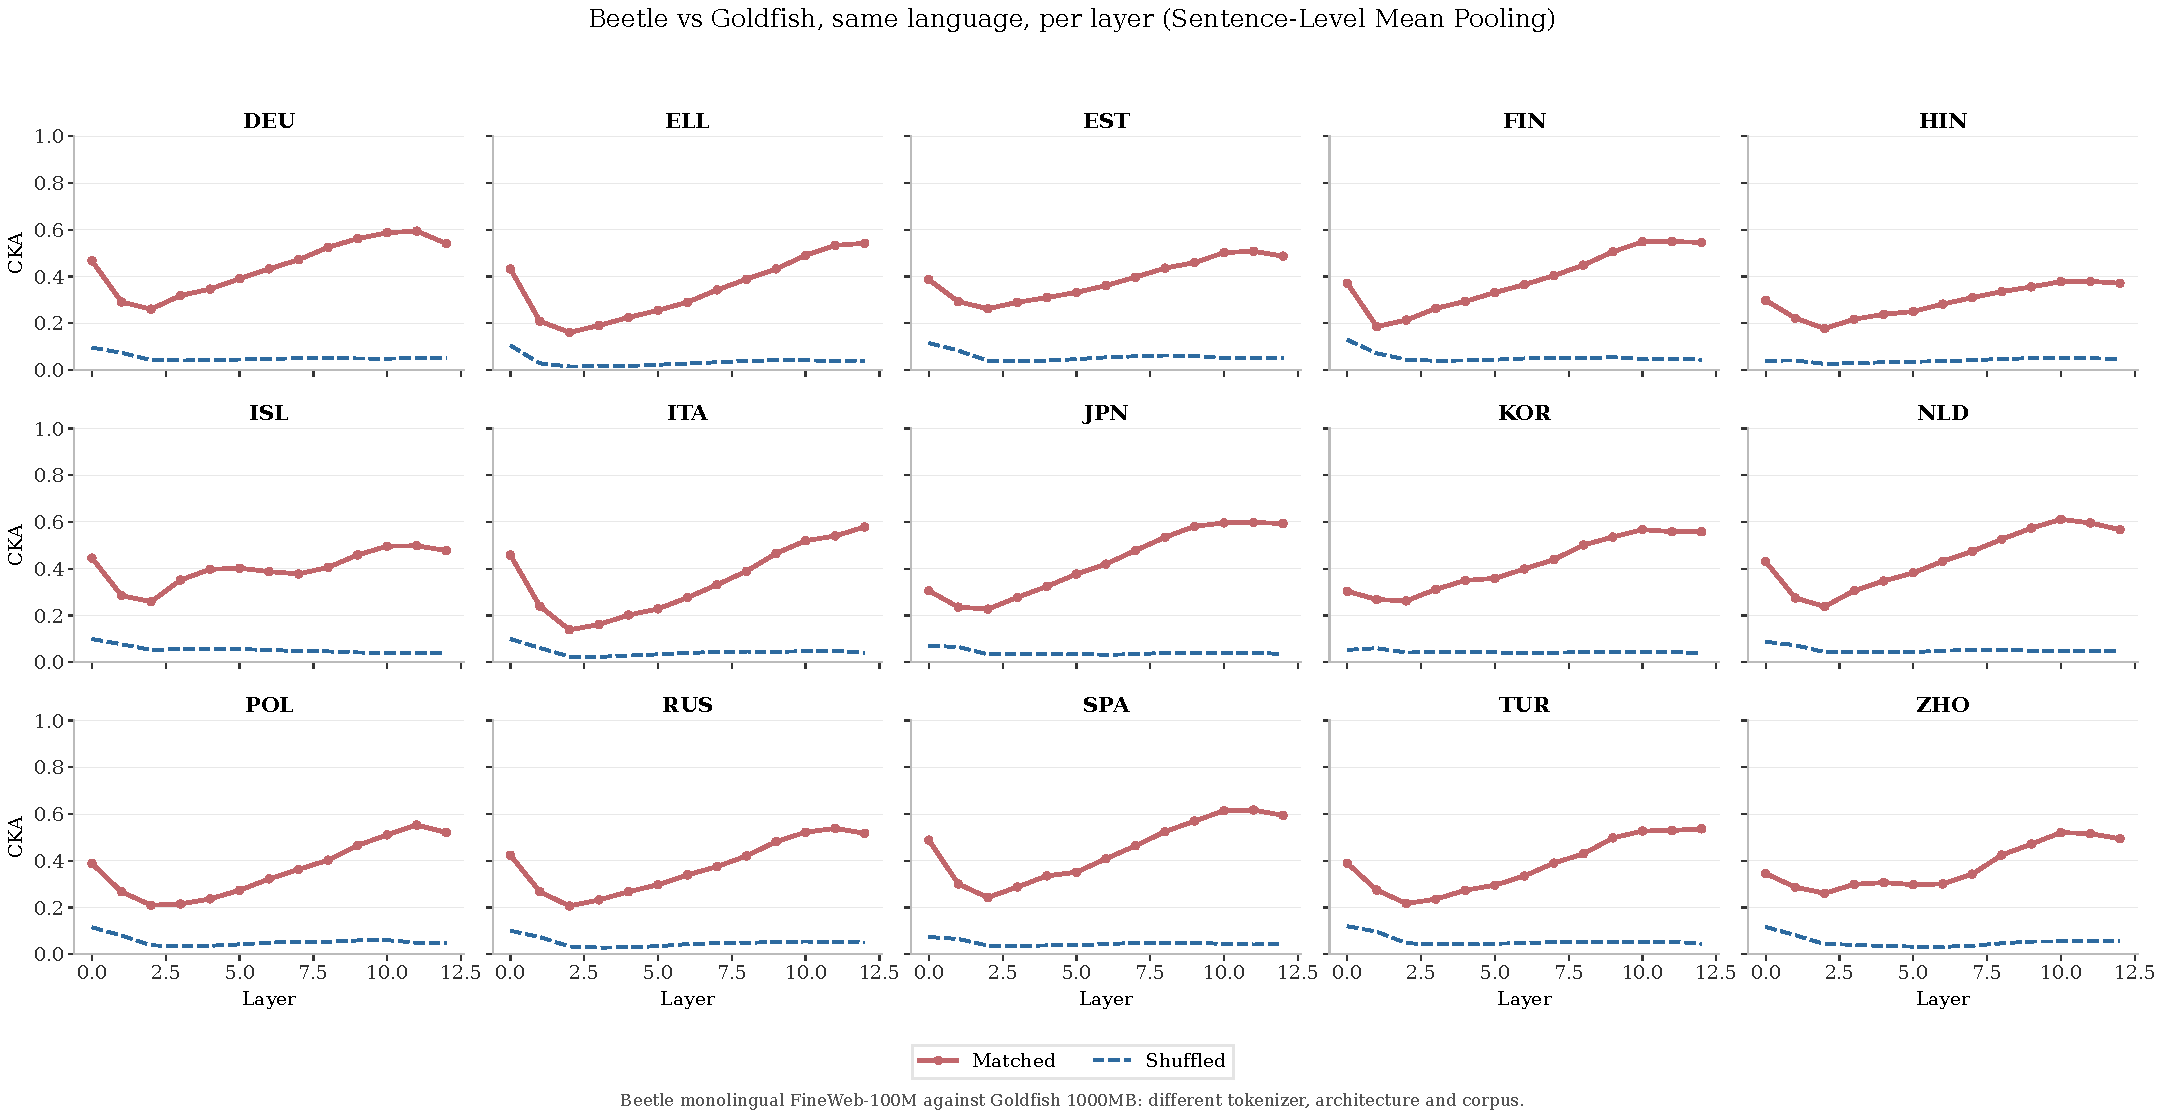
\includegraphics[width=\textwidth,height=0.74\textheight,keepaspectratio]{figures/gfE10_beetle_vs_goldfish_mean_pool.pdf}
  \end{center}
  \vspace{-0.5em}\begin{center}\tiny {\tiny\texttt{\detokenize{gfE10_beetle_vs_goldfish_mean_pool.pdf}}}\end{center}
\end{frame}

\begin{frame}{gfE10: Beetle vs goldfish SGPT pooling}
  \begin{center}
    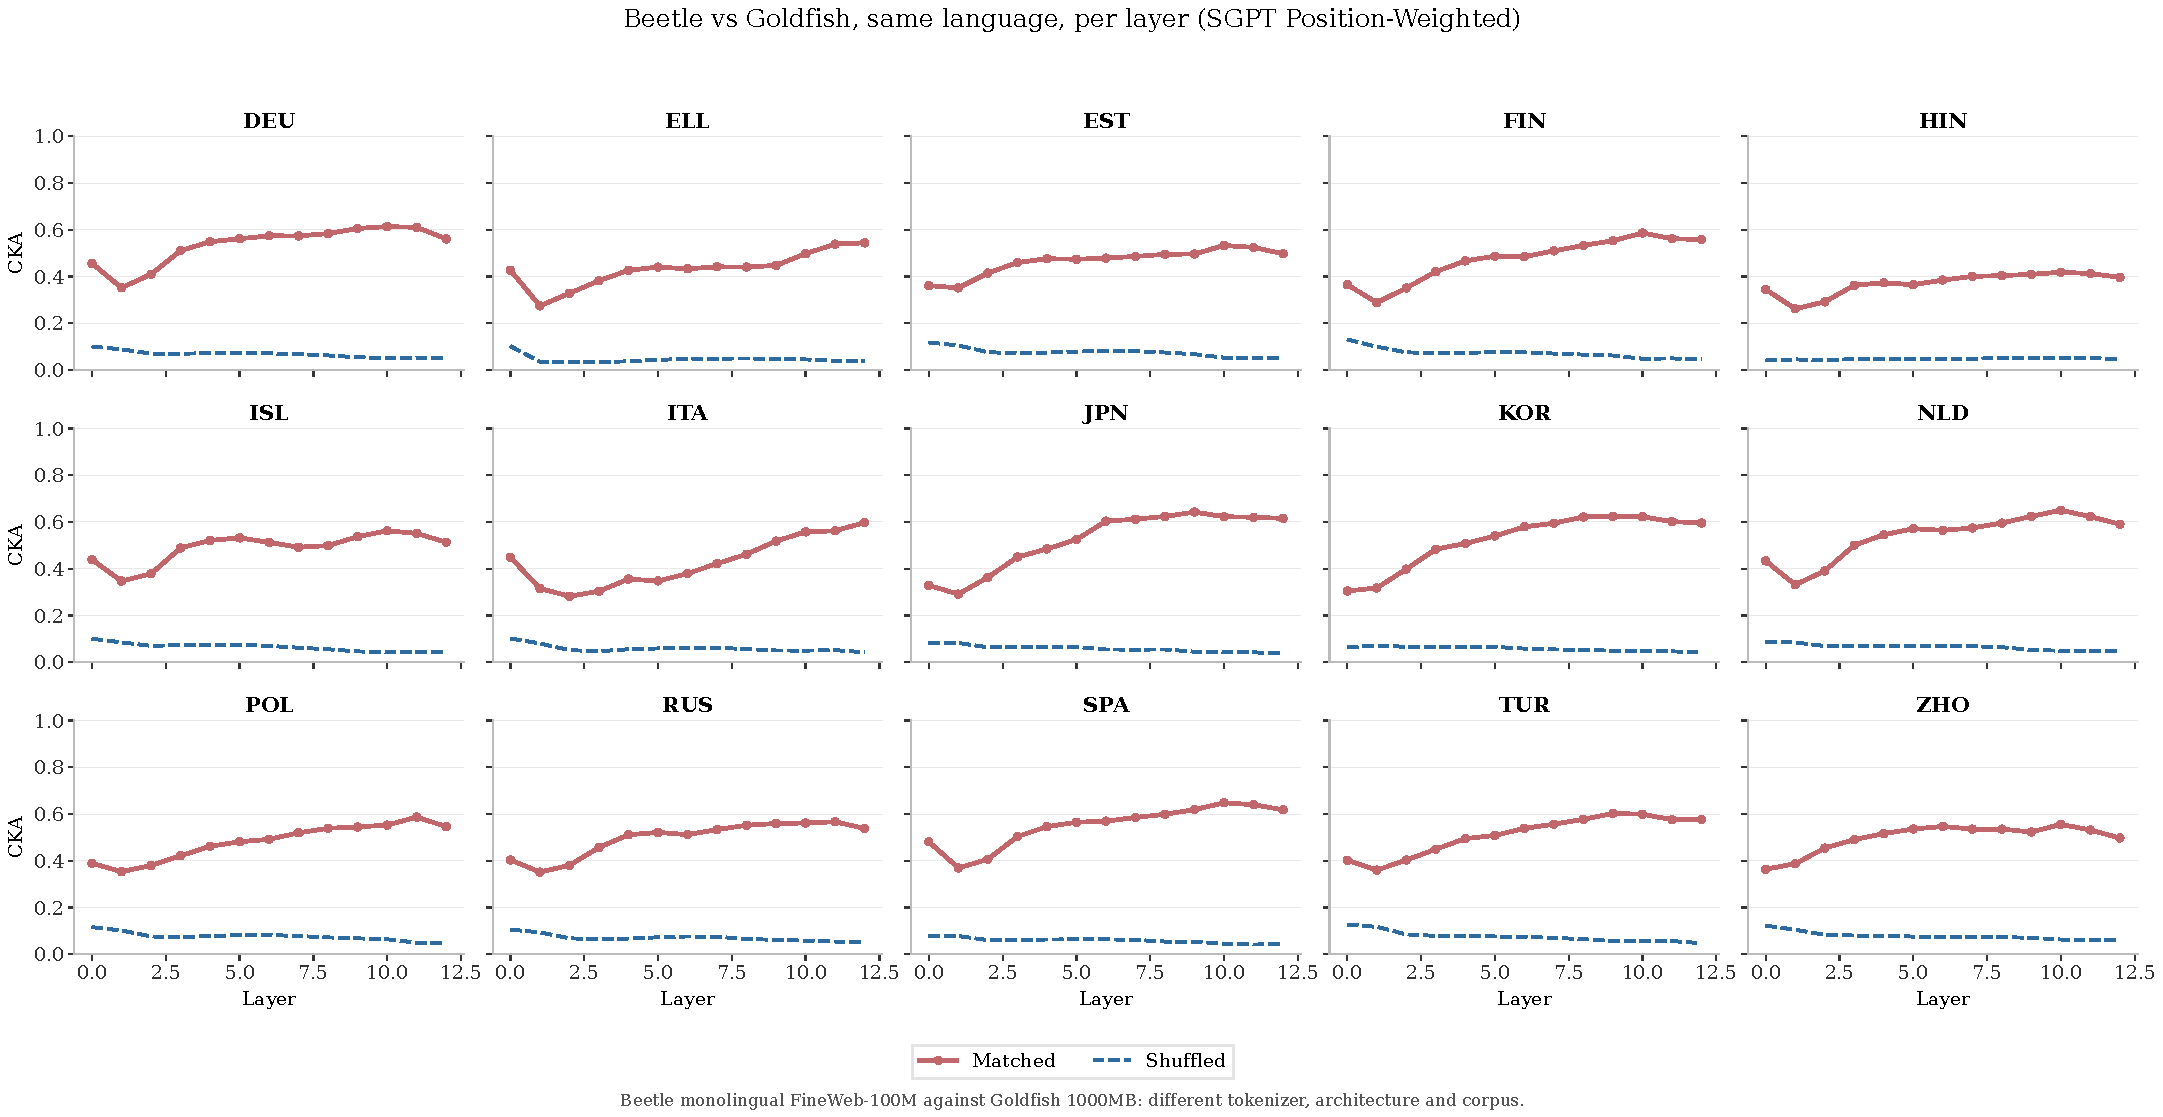
\includegraphics[width=\textwidth,height=0.74\textheight,keepaspectratio]{figures/gfE10_beetle_vs_goldfish_sgpt.pdf}
  \end{center}
  \vspace{-0.5em}\begin{center}\tiny {\tiny\texttt{\detokenize{gfE10_beetle_vs_goldfish_sgpt.pdf}}}\end{center}
\end{frame}

\begin{frame}{gfE10: Beetle vs goldfish token aligned}
  \begin{center}
    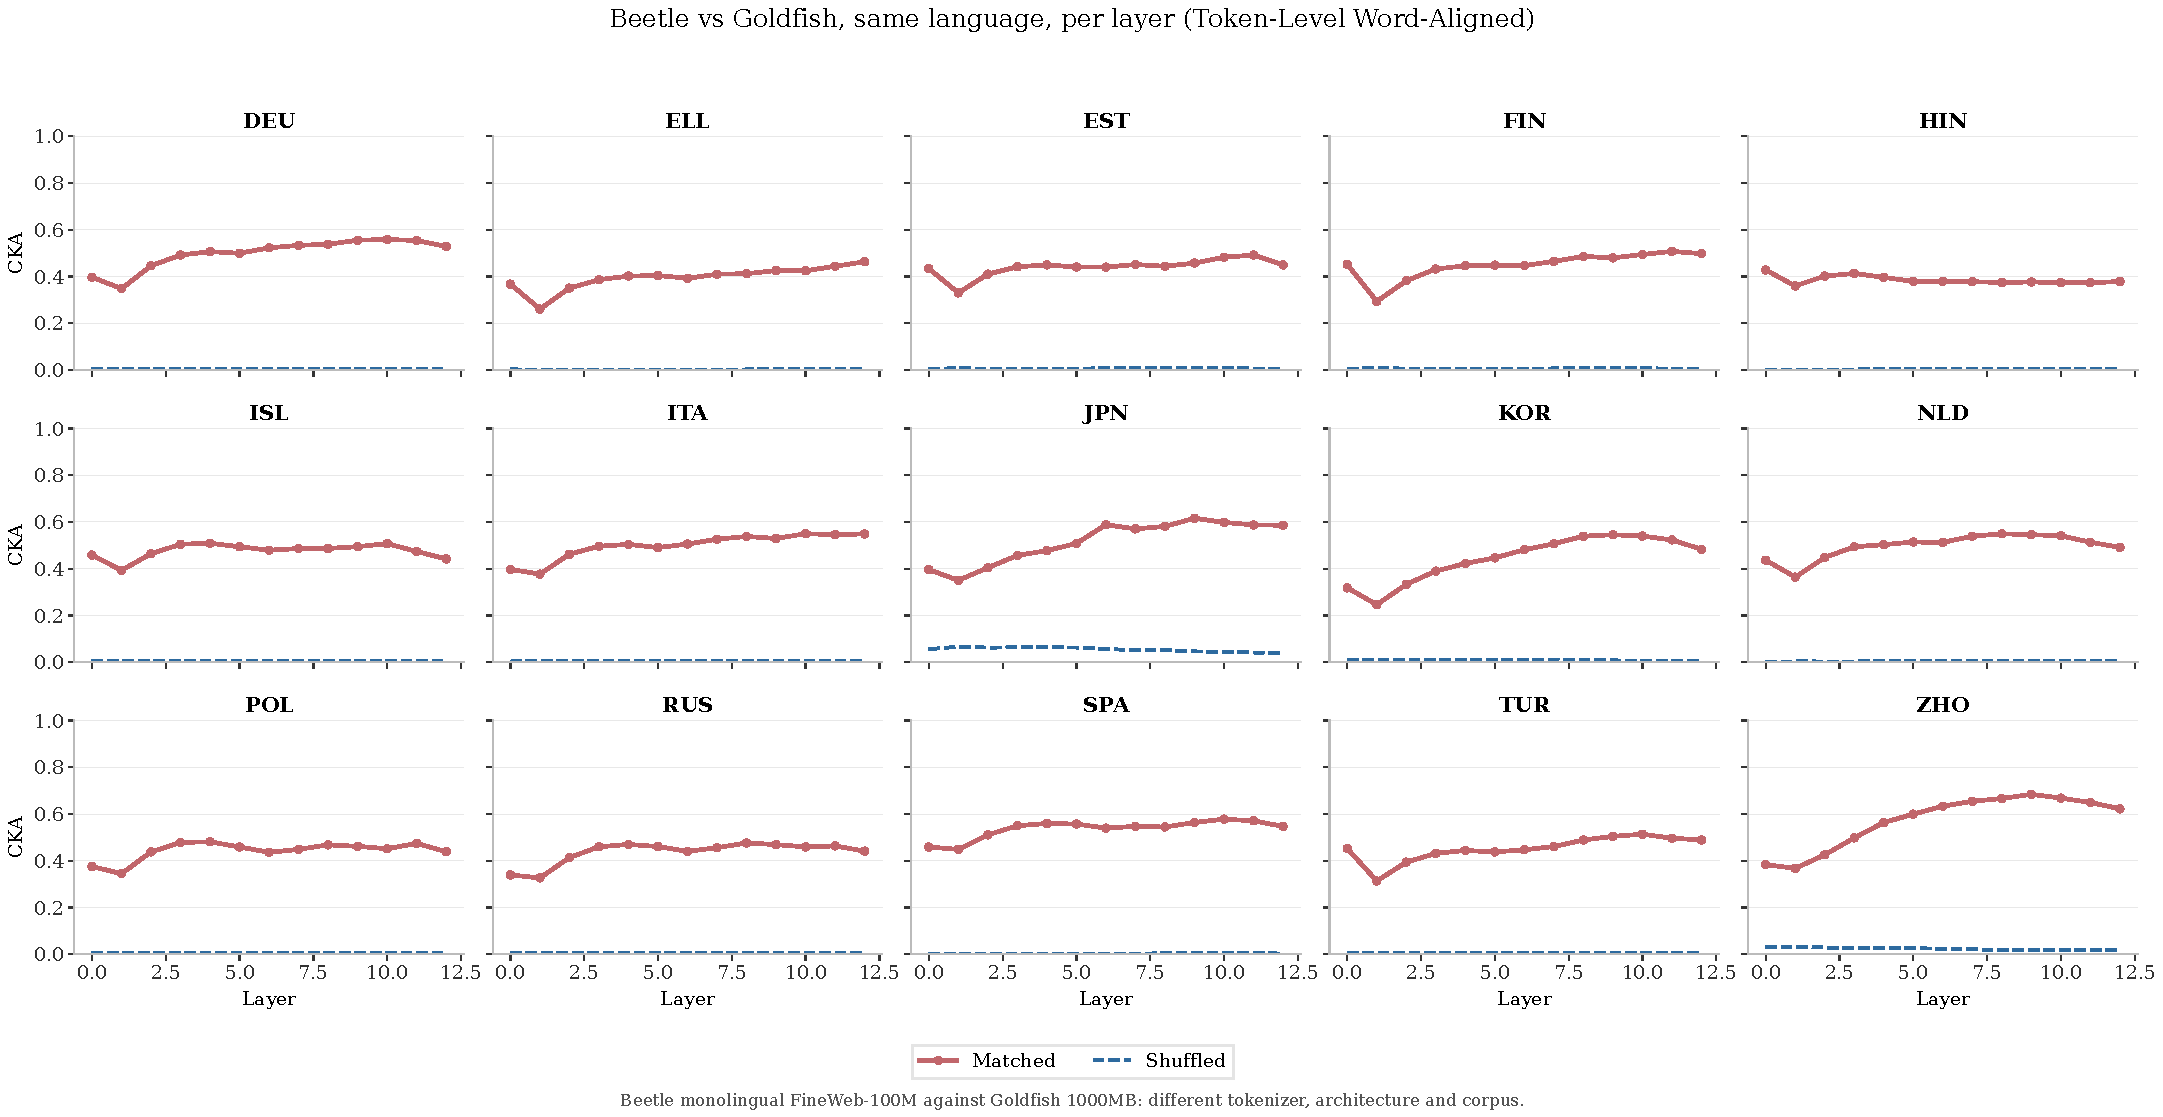
\includegraphics[width=\textwidth,height=0.74\textheight,keepaspectratio]{figures/gfE10_beetle_vs_goldfish_token_aligned.pdf}
  \end{center}
  \vspace{-0.5em}\begin{center}\tiny {\tiny\texttt{\detokenize{gfE10_beetle_vs_goldfish_token_aligned.pdf}}}\end{center}
\end{frame}

\subsection{Curriculum and scale grids}

\begin{frame}{gfE14: Crossing l1 curriculum}
  \begin{center}
    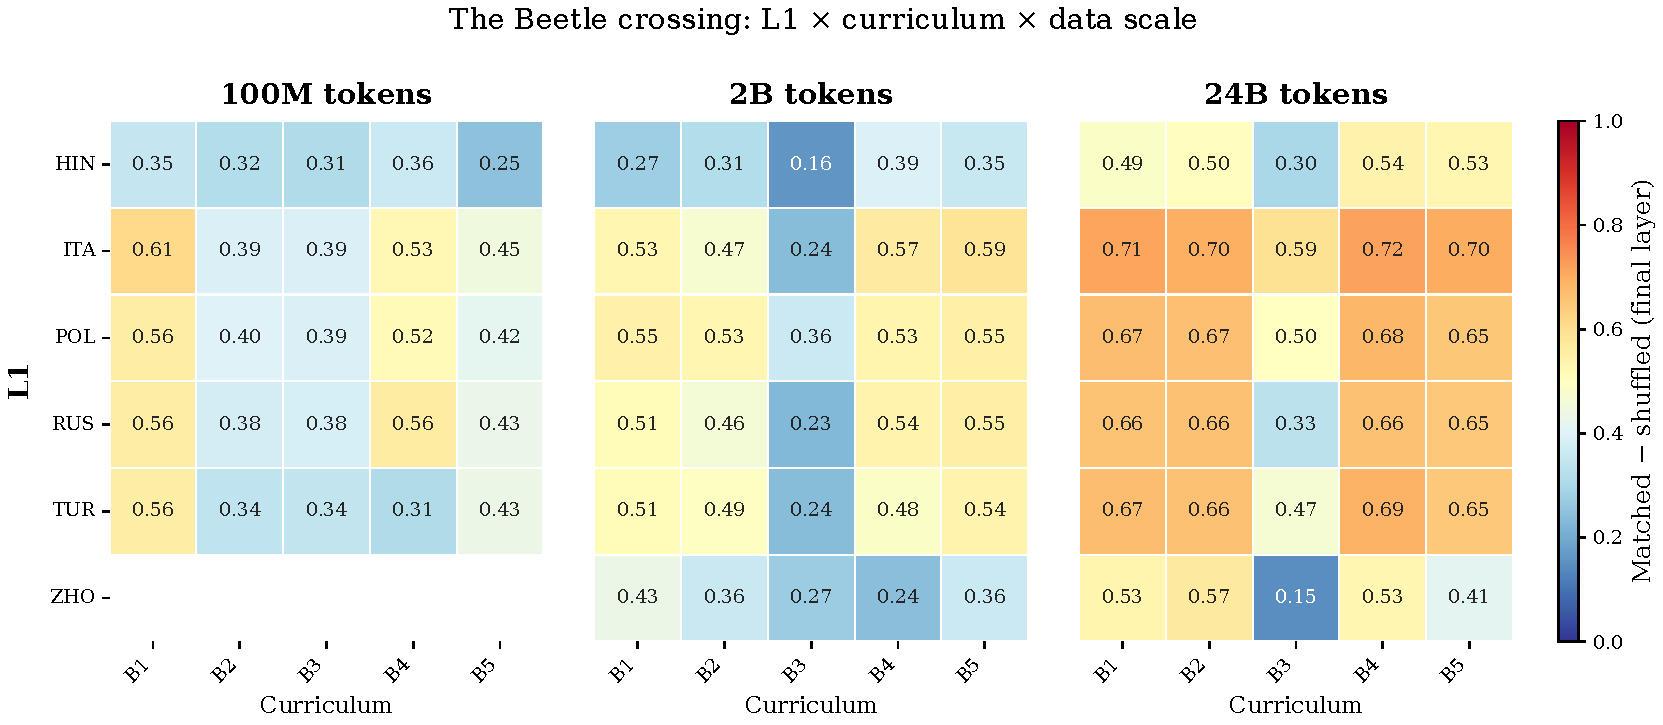
\includegraphics[width=\textwidth,height=0.74\textheight,keepaspectratio]{figures/gfE14_crossing_l1_curriculum.pdf}
  \end{center}
  \vspace{-0.5em}\begin{center}\tiny {\tiny\texttt{\detokenize{gfE14_crossing_l1_curriculum.pdf}}}\end{center}
\end{frame}

\begin{frame}{gfE14: Grid by curriculum}
  \begin{center}
    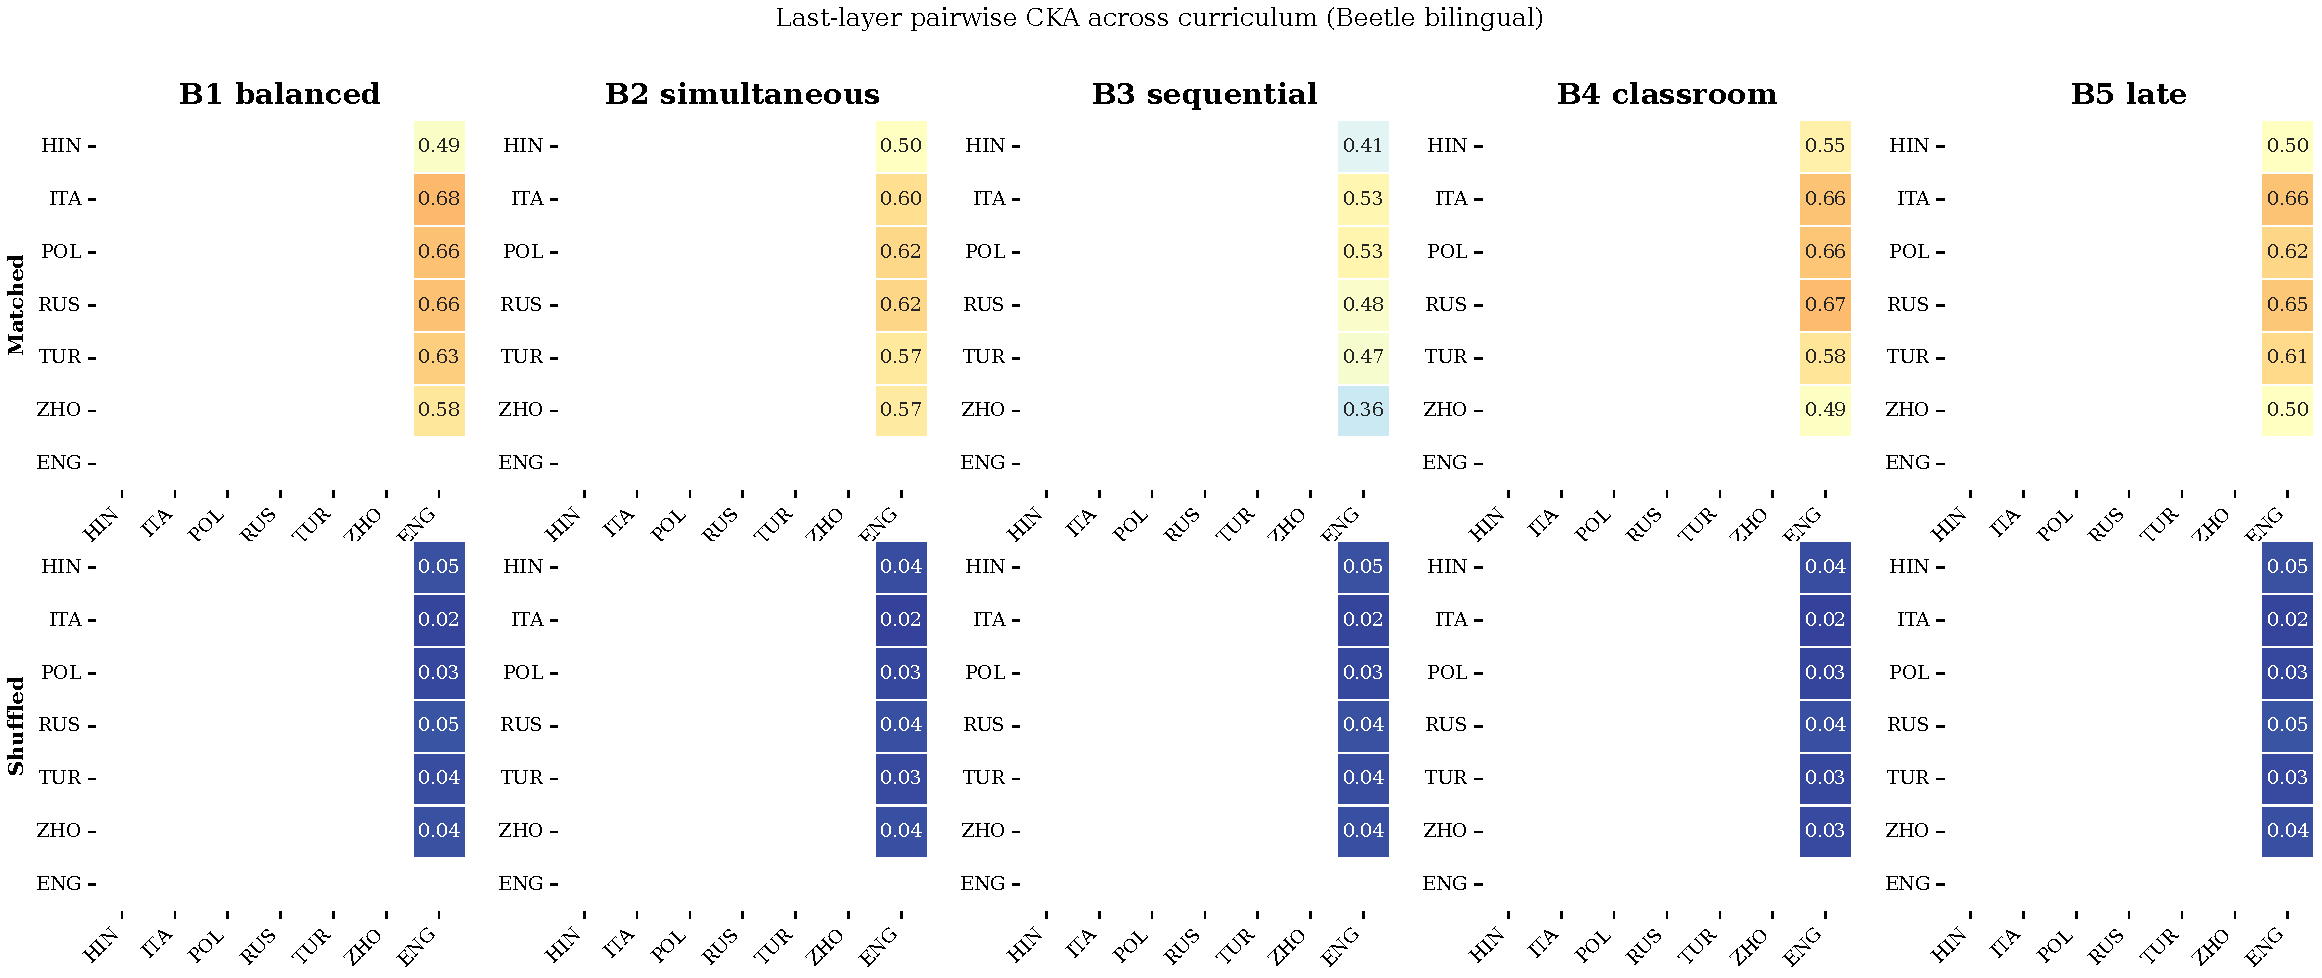
\includegraphics[width=\textwidth,height=0.74\textheight,keepaspectratio]{figures/gfE14_grid_by_curriculum.pdf}
  \end{center}
  \vspace{-0.5em}\begin{center}\tiny {\tiny\texttt{\detokenize{gfE14_grid_by_curriculum.pdf}}}\end{center}
\end{frame}

\begin{frame}{gfE14: Grid by scale}
  \begin{center}
    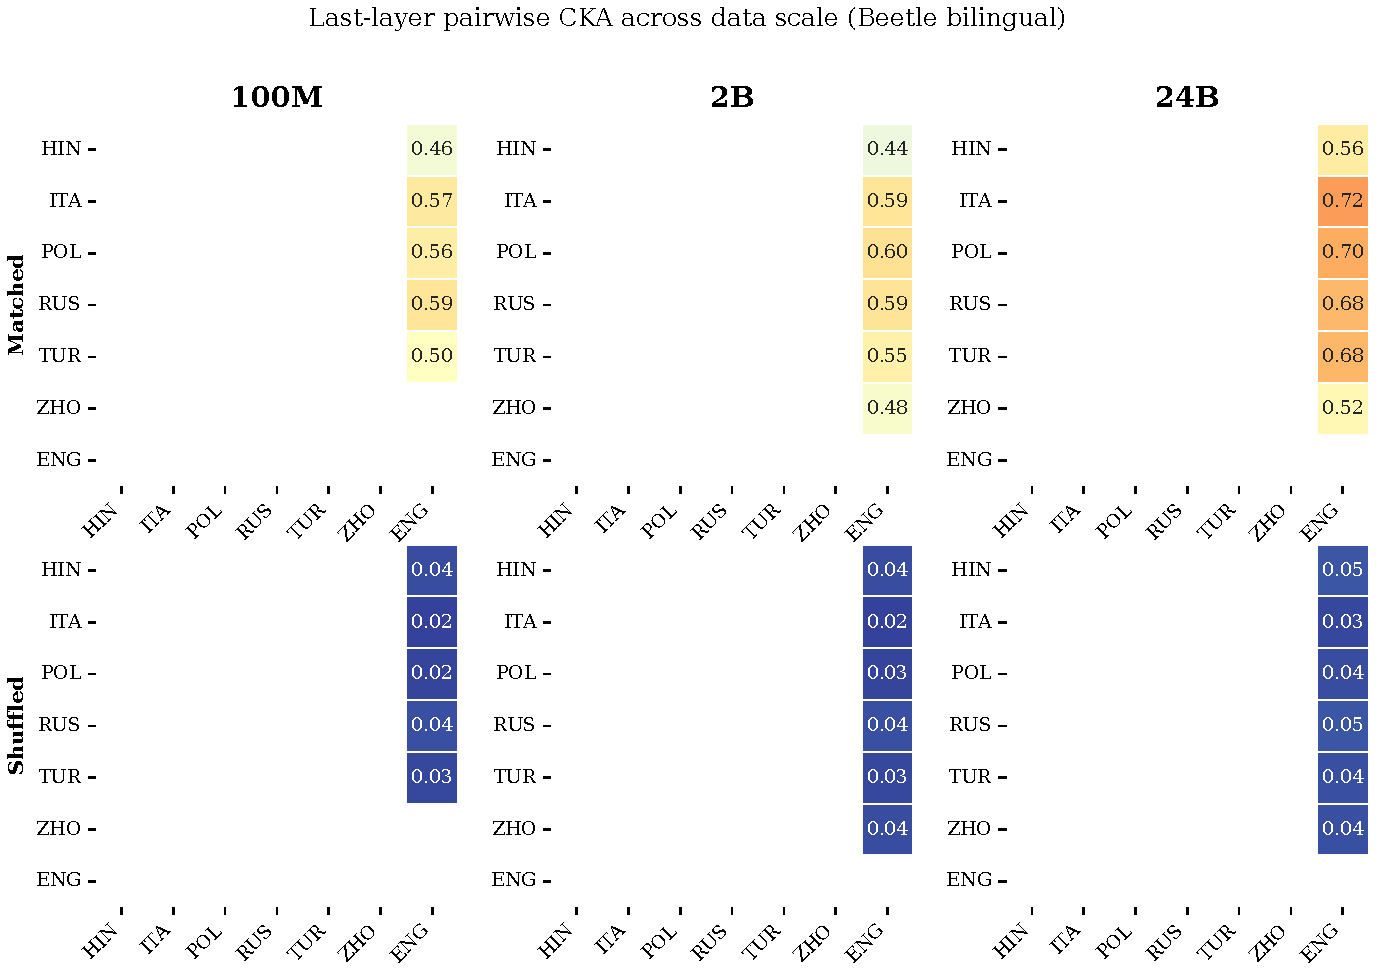
\includegraphics[width=\textwidth,height=0.74\textheight,keepaspectratio]{figures/gfE14_grid_by_scale.pdf}
  \end{center}
  \vspace{-0.5em}\begin{center}\tiny {\tiny\texttt{\detokenize{gfE14_grid_by_scale.pdf}}}\end{center}
\end{frame}

\begin{frame}{gfE14: Grid mono}
  \begin{center}
    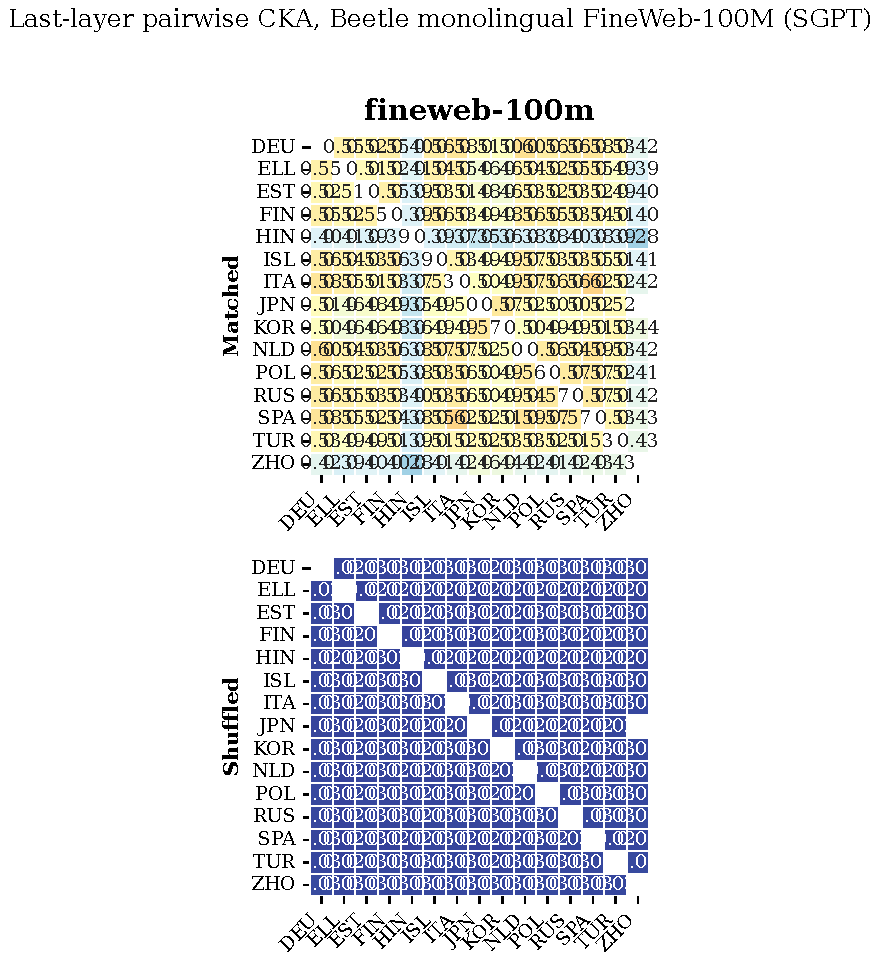
\includegraphics[width=\textwidth,height=0.74\textheight,keepaspectratio]{figures/gfE14_grid_mono.pdf}
  \end{center}
  \vspace{-0.5em}\begin{center}\tiny {\tiny\texttt{\detokenize{gfE14_grid_mono.pdf}}}\end{center}
\end{frame}

\begin{frame}{gfE14: Matrix mean pool}
  \begin{center}
    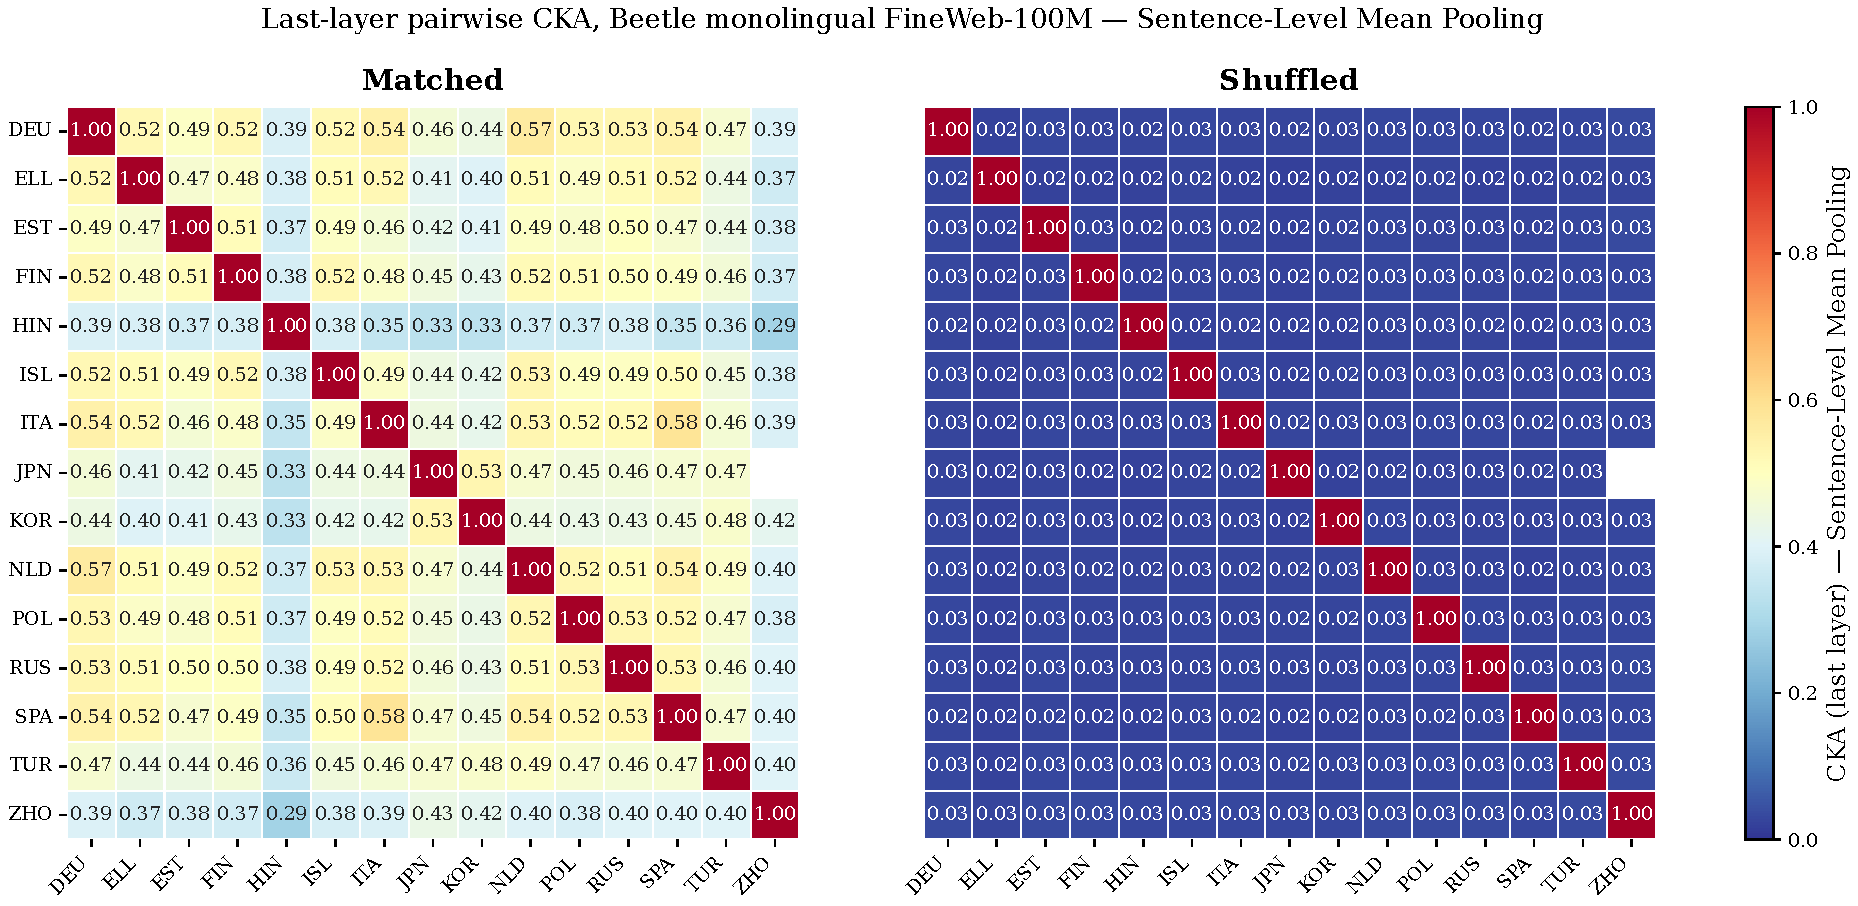
\includegraphics[width=\textwidth,height=0.74\textheight,keepaspectratio]{figures/gfE14_matrix_mean_pool.pdf}
  \end{center}
  \vspace{-0.5em}\begin{center}\tiny {\tiny\texttt{\detokenize{gfE14_matrix_mean_pool.pdf}}}\end{center}
\end{frame}

\begin{frame}{gfE14: Matrix SGPT pooling}
  \begin{center}
    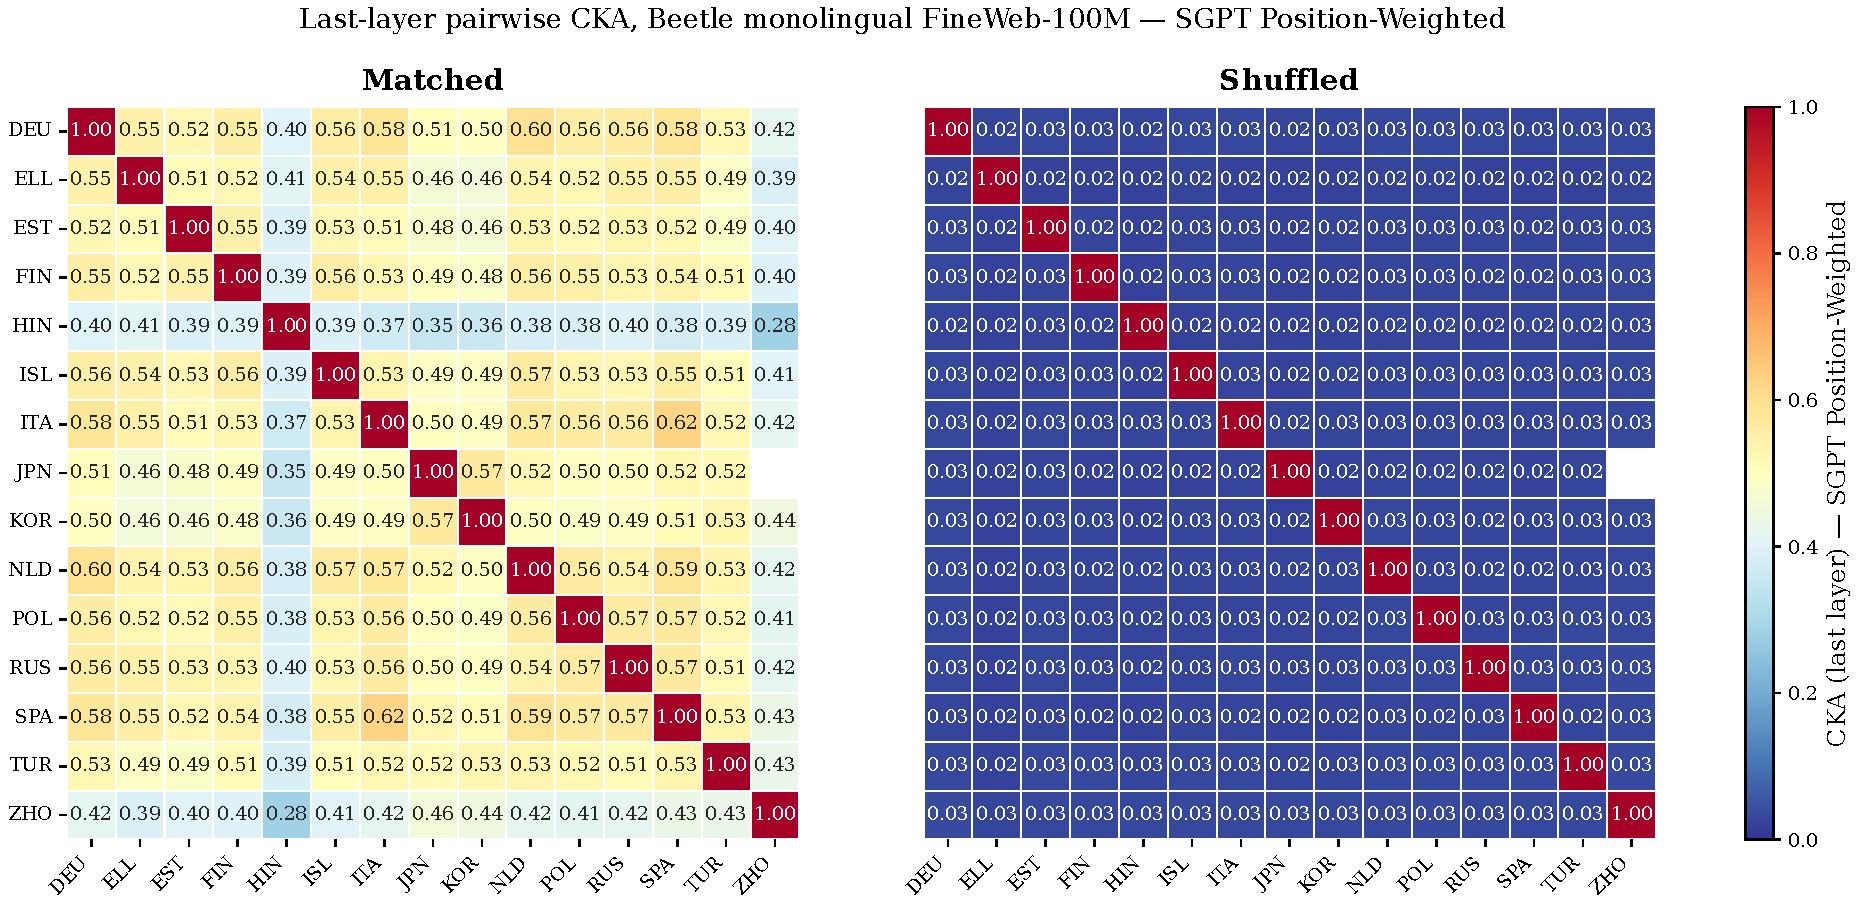
\includegraphics[width=\textwidth,height=0.74\textheight,keepaspectratio]{figures/gfE14_matrix_sgpt.pdf}
  \end{center}
  \vspace{-0.5em}\begin{center}\tiny {\tiny\texttt{\detokenize{gfE14_matrix_sgpt.pdf}}}\end{center}
\end{frame}

\begin{frame}{gfE14: Matrix token aligned}
  \begin{center}
    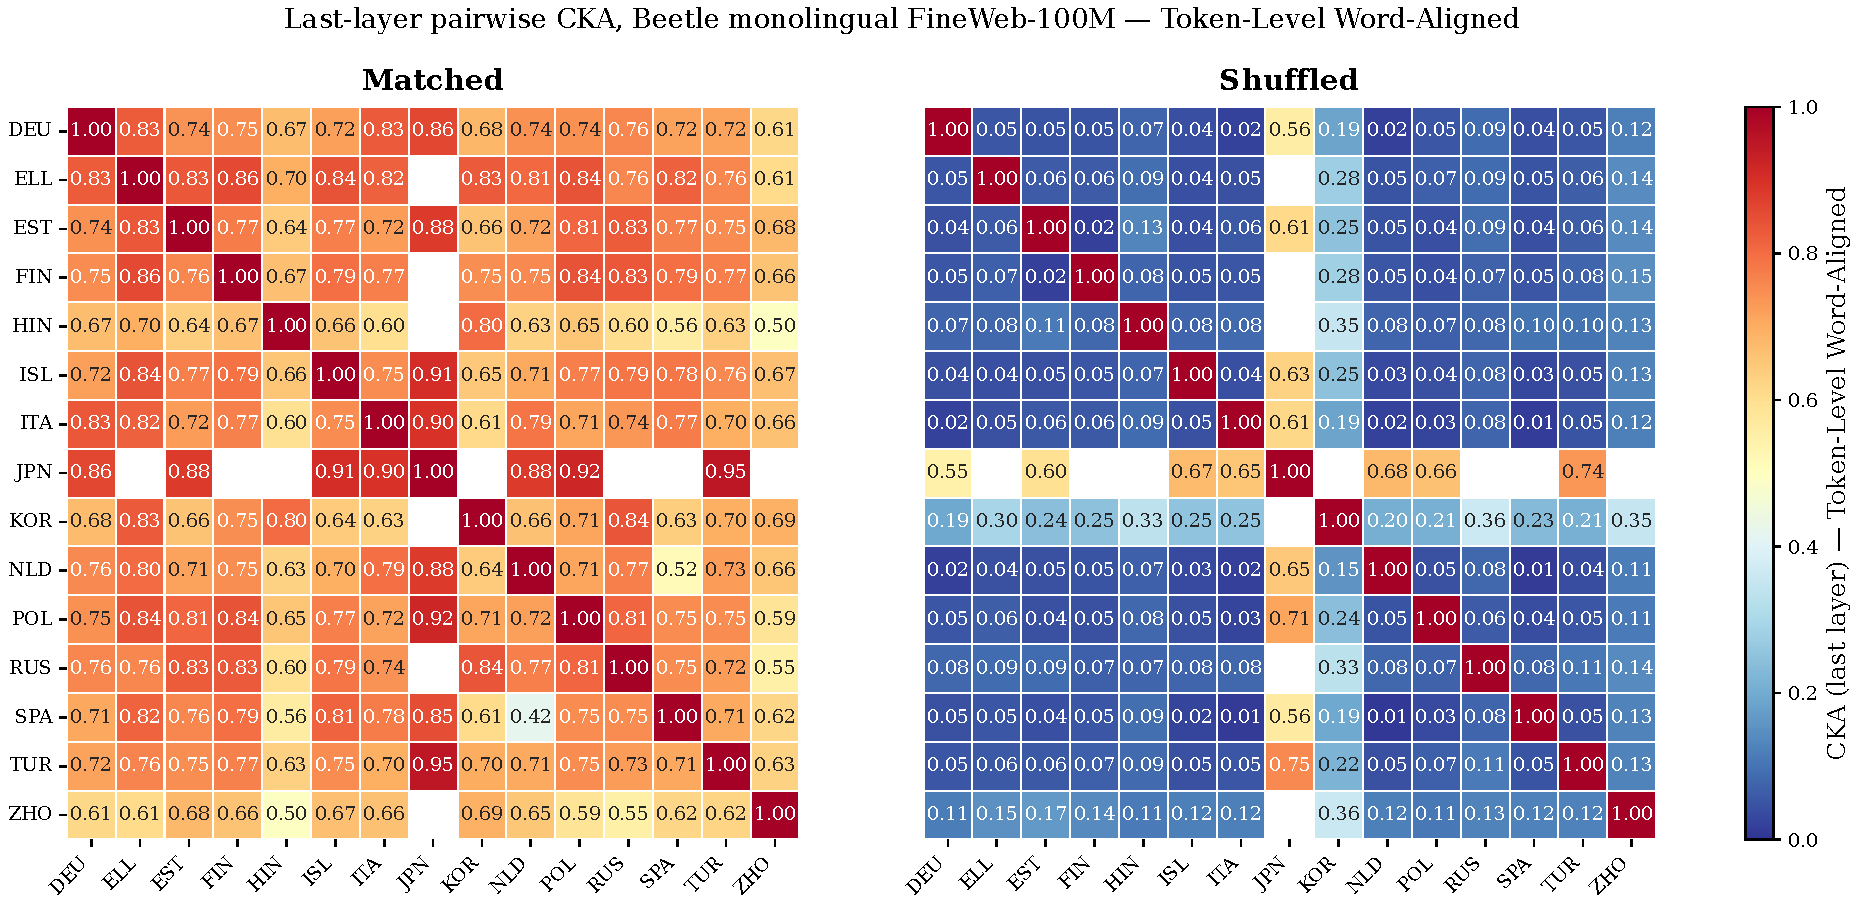
\includegraphics[width=\textwidth,height=0.74\textheight,keepaspectratio]{figures/gfE14_matrix_token_aligned.pdf}
  \end{center}
  \vspace{-0.5em}\begin{center}\tiny {\tiny\texttt{\detokenize{gfE14_matrix_token_aligned.pdf}}}\end{center}
\end{frame}

\subsection{PCA grids}

\begin{frame}{gfE18: PCA grid eng deu}
  \begin{center}
    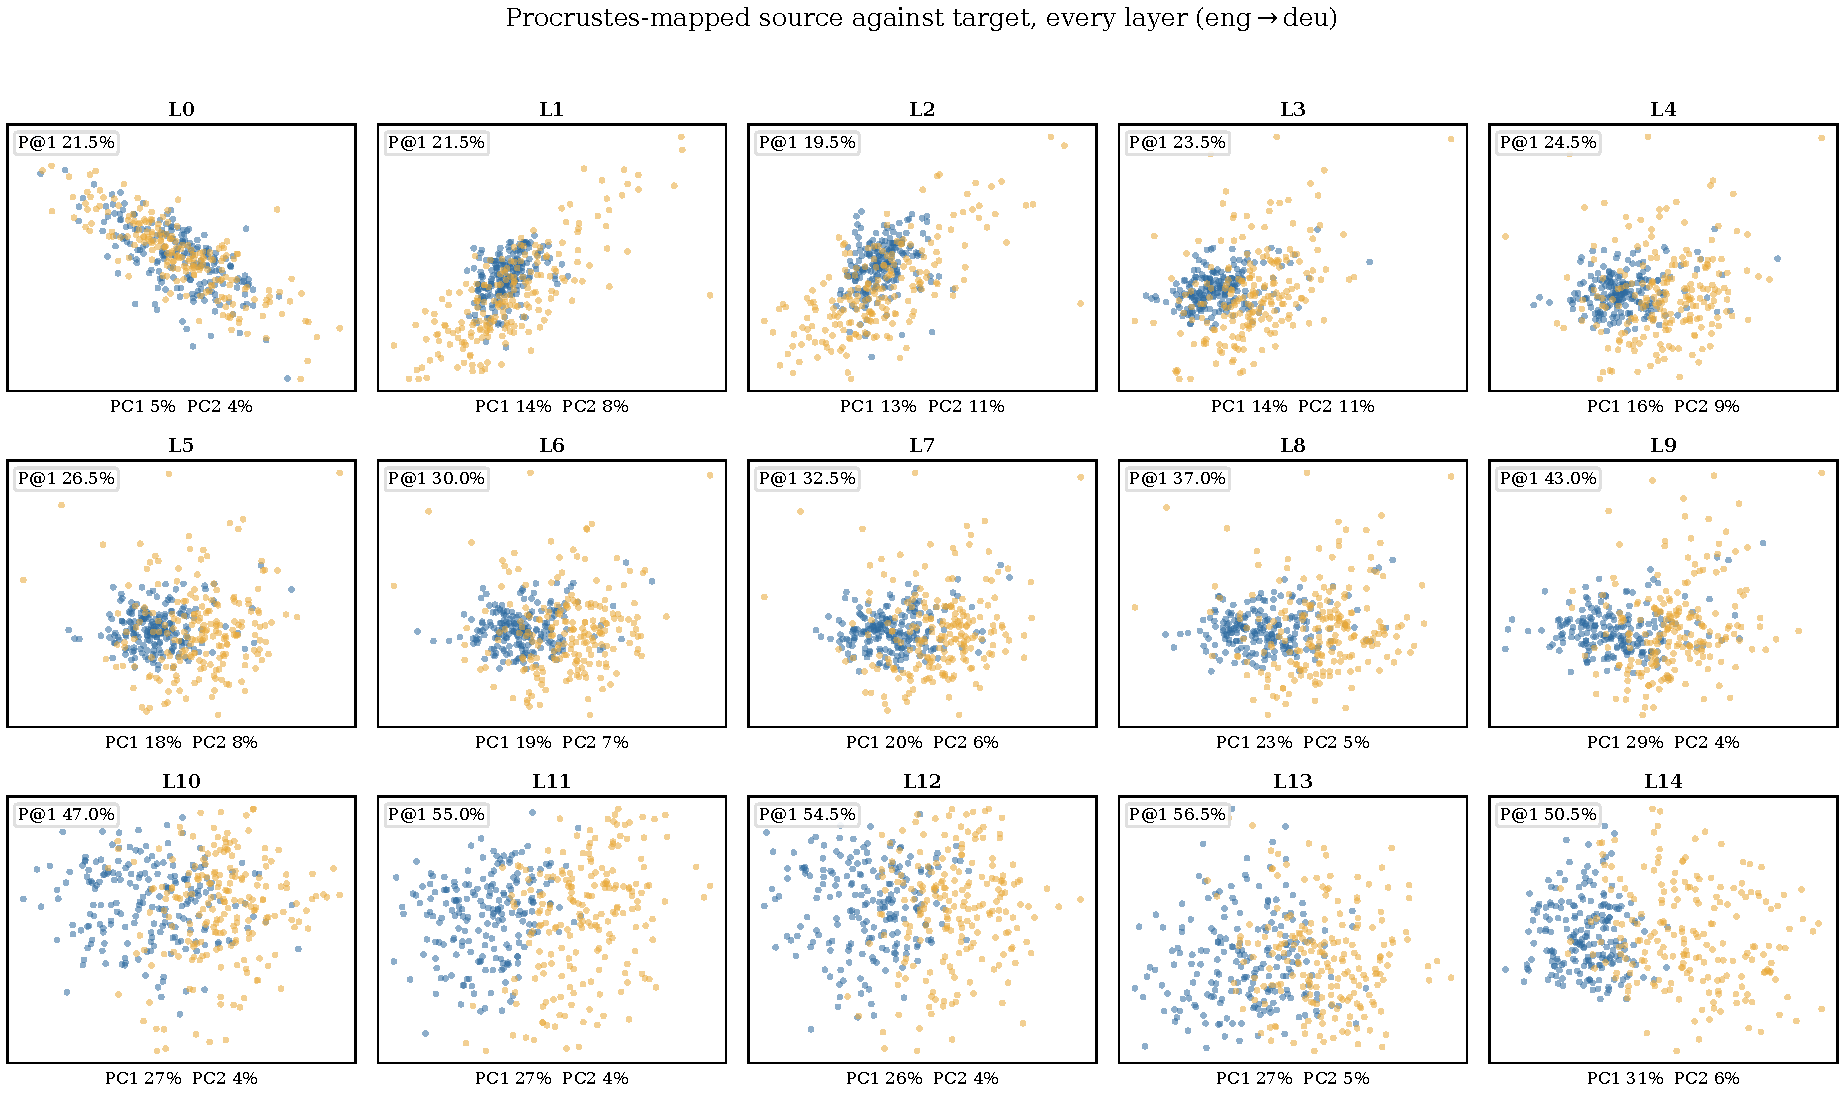
\includegraphics[width=\textwidth,height=0.74\textheight,keepaspectratio]{figures/gfE18_pca_grid_eng_deu.pdf}
  \end{center}
  \vspace{-0.5em}\begin{center}\tiny {\tiny\texttt{\detokenize{gfE18_pca_grid_eng_deu.pdf}}}\end{center}
\end{frame}

\begin{frame}{gfE18: PCA grid eng nld}
  \begin{center}
    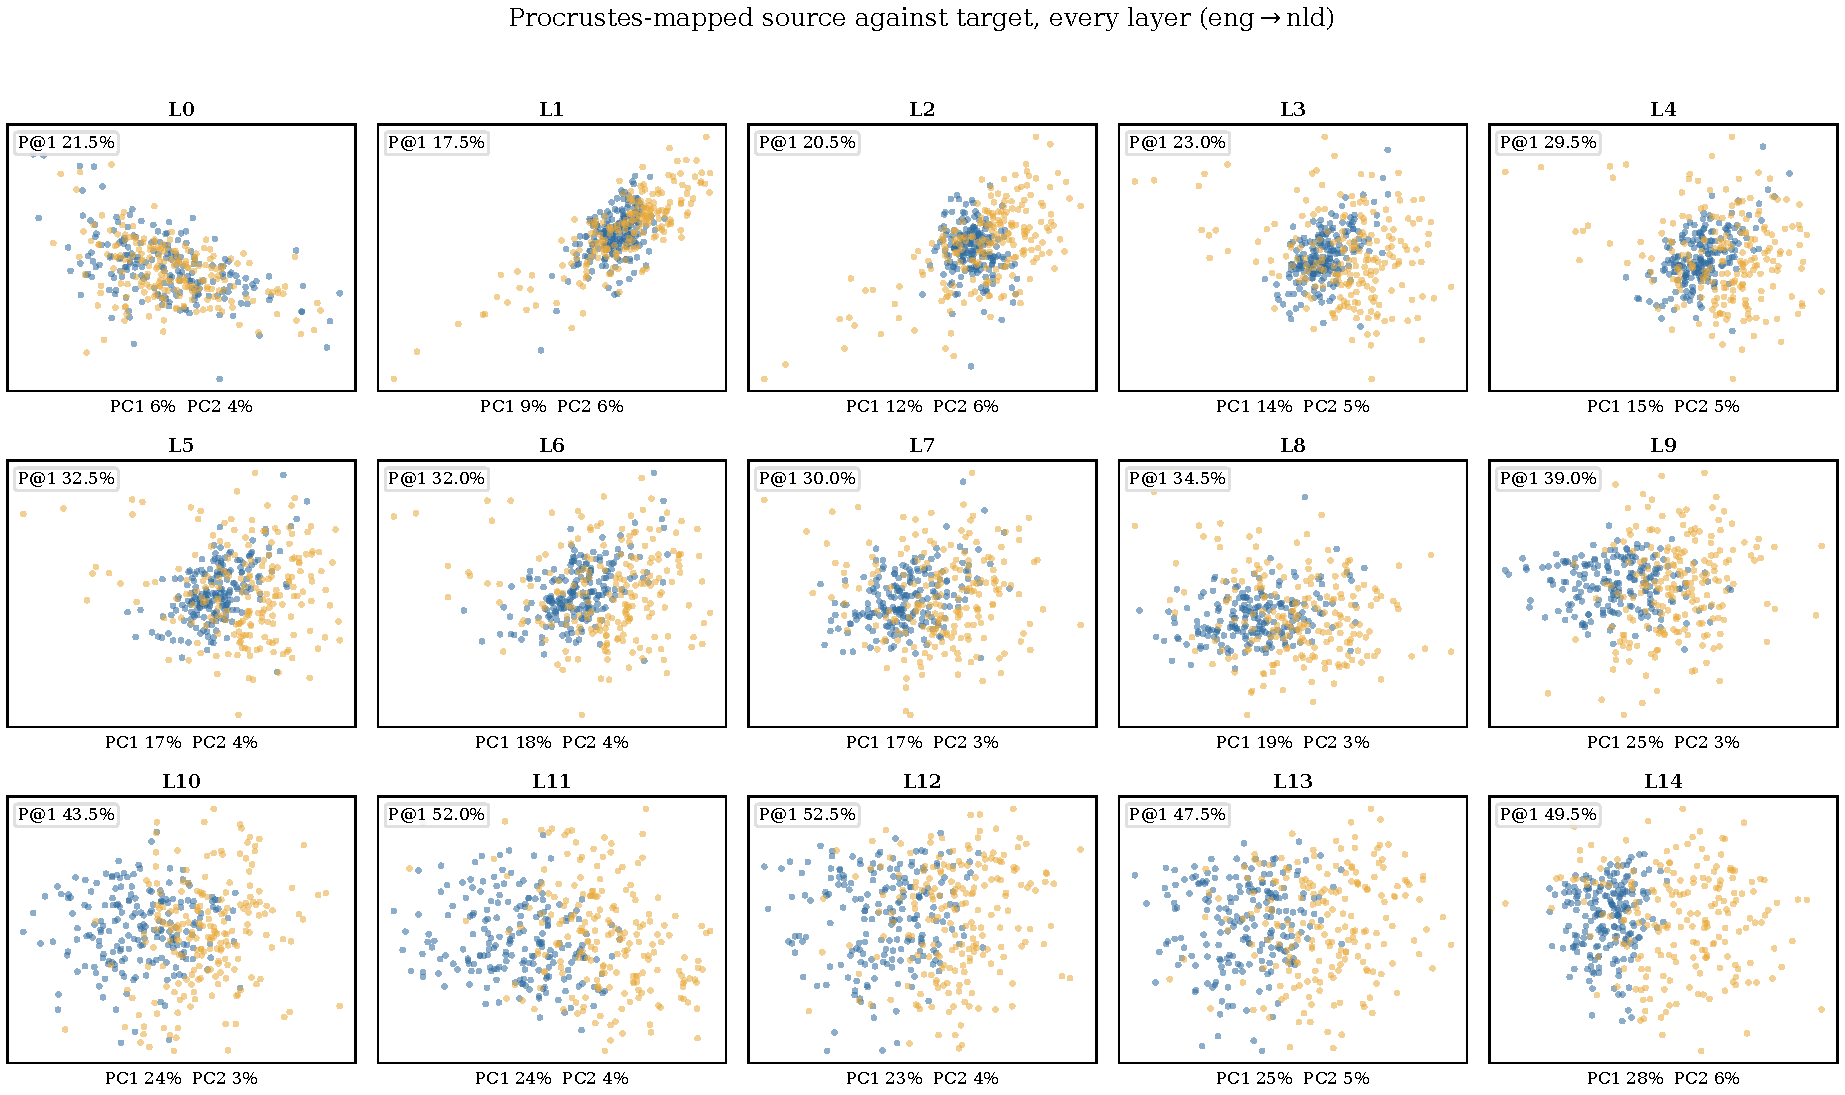
\includegraphics[width=\textwidth,height=0.74\textheight,keepaspectratio]{figures/gfE18_pca_grid_eng_nld.pdf}
  \end{center}
  \vspace{-0.5em}\begin{center}\tiny {\tiny\texttt{\detokenize{gfE18_pca_grid_eng_nld.pdf}}}\end{center}
\end{frame}

\begin{frame}{gfE18: PCA grid eng zho}
  \begin{center}
    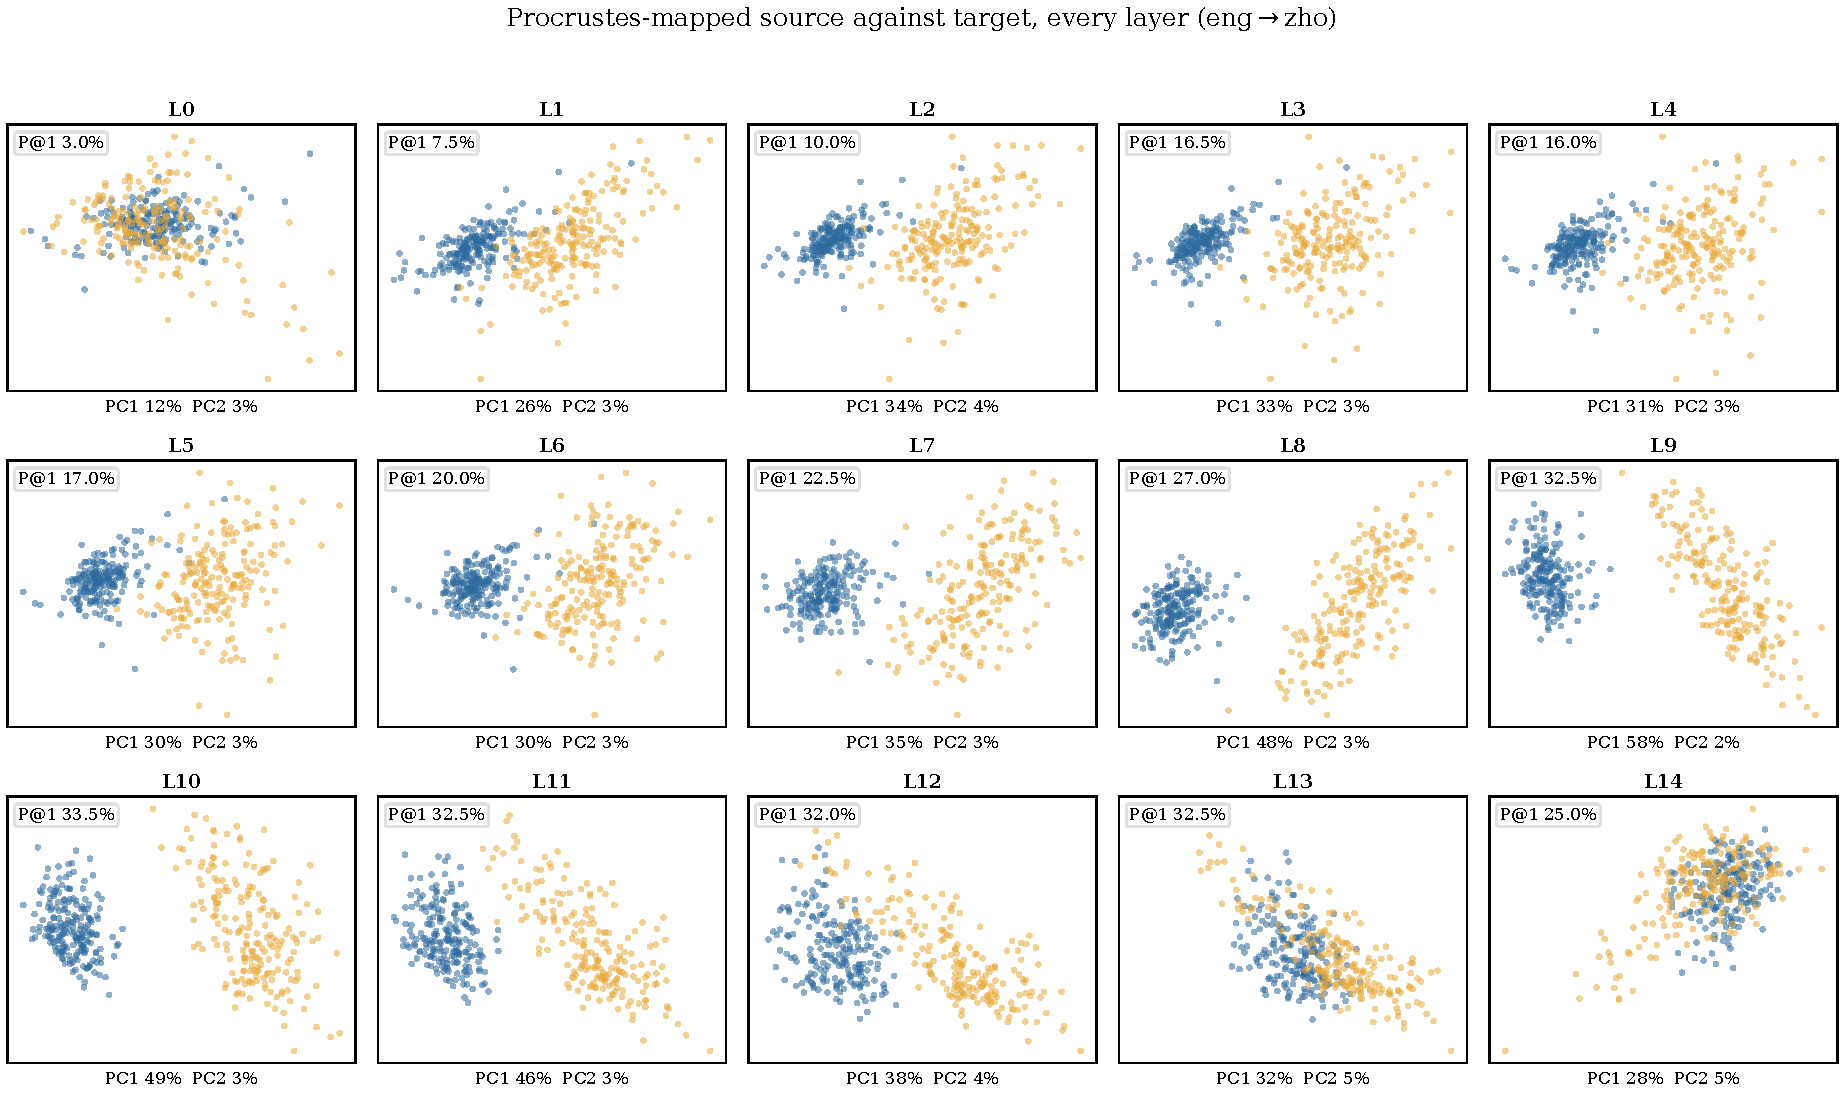
\includegraphics[width=\textwidth,height=0.74\textheight,keepaspectratio]{figures/gfE18_pca_grid_eng_zho.pdf}
  \end{center}
  \vspace{-0.5em}\begin{center}\tiny {\tiny\texttt{\detokenize{gfE18_pca_grid_eng_zho.pdf}}}\end{center}
\end{frame}

\begin{frame}{gfE18: PCA grid nld deu}
  \begin{center}
    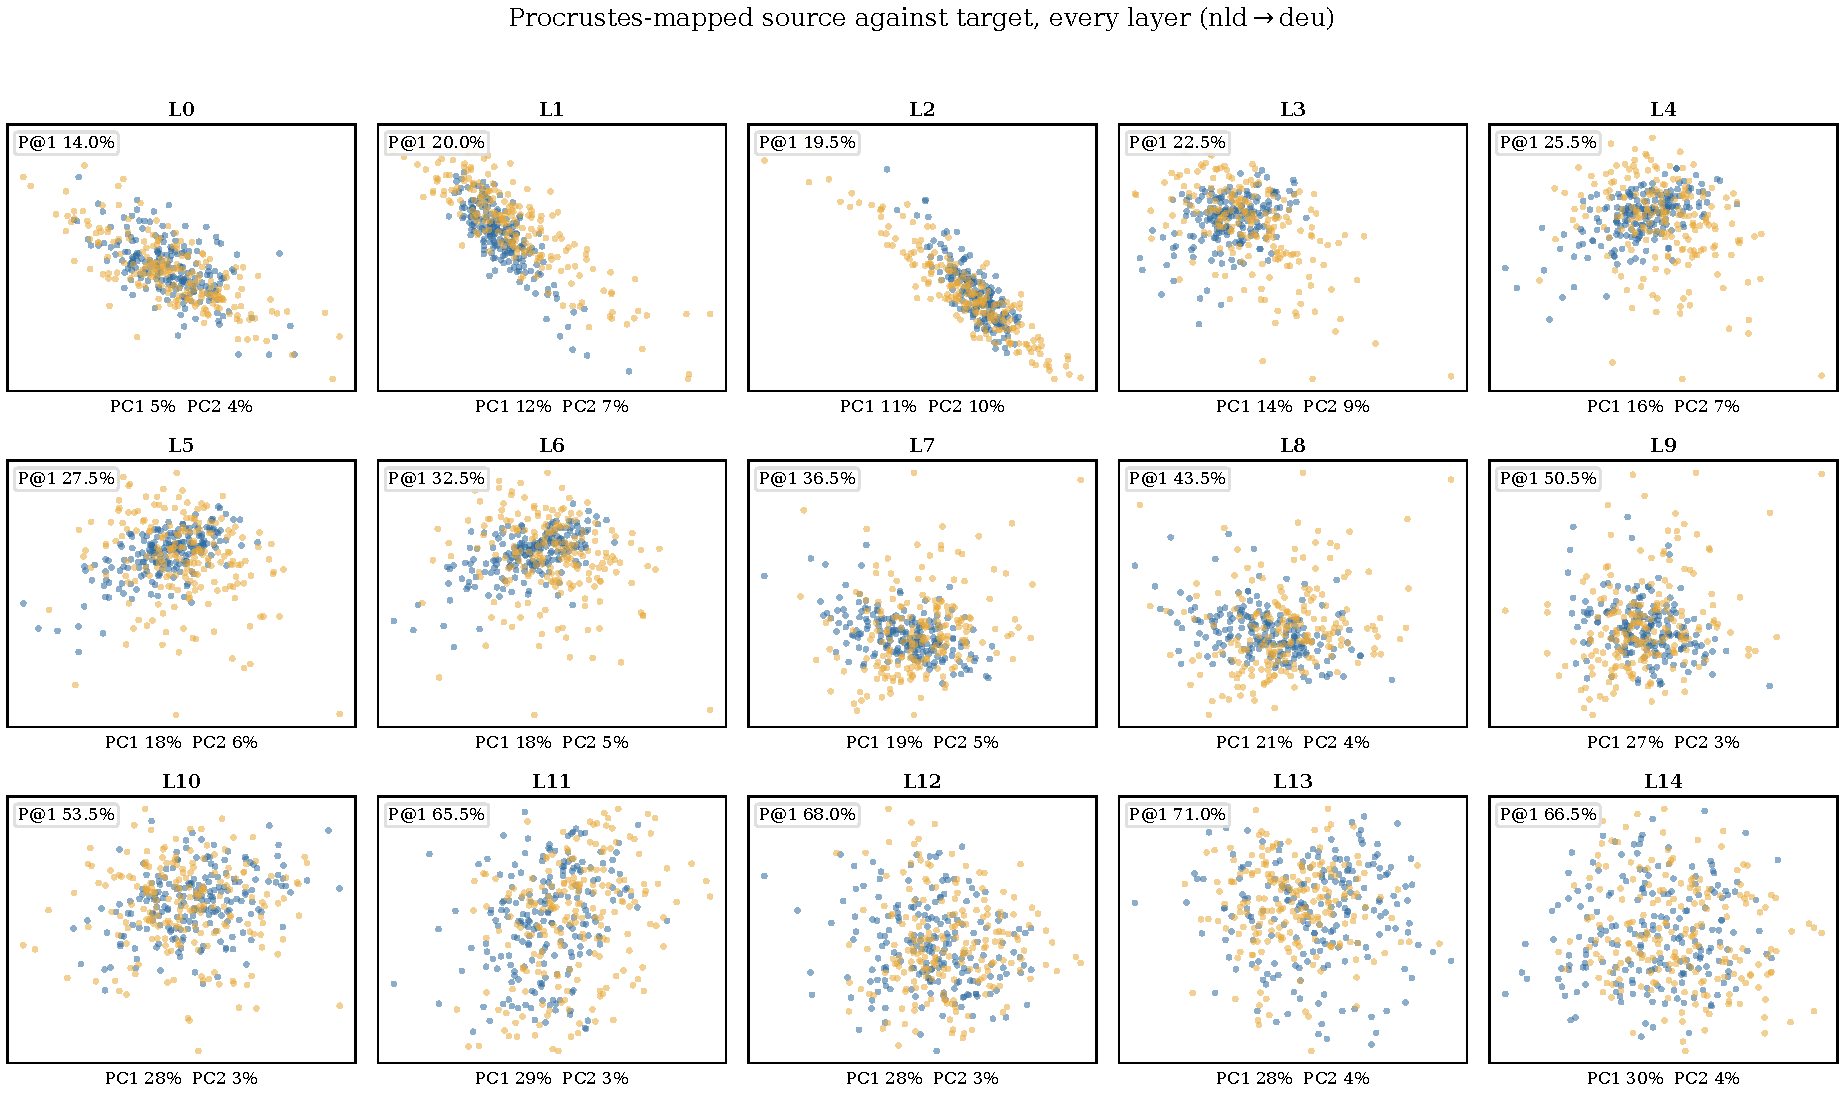
\includegraphics[width=\textwidth,height=0.74\textheight,keepaspectratio]{figures/gfE18_pca_grid_nld_deu.pdf}
  \end{center}
  \vspace{-0.5em}\begin{center}\tiny {\tiny\texttt{\detokenize{gfE18_pca_grid_nld_deu.pdf}}}\end{center}
\end{frame}

\section{Additional panels}

\begin{frame}{Slides fig10 horse race}
  \begin{center}
    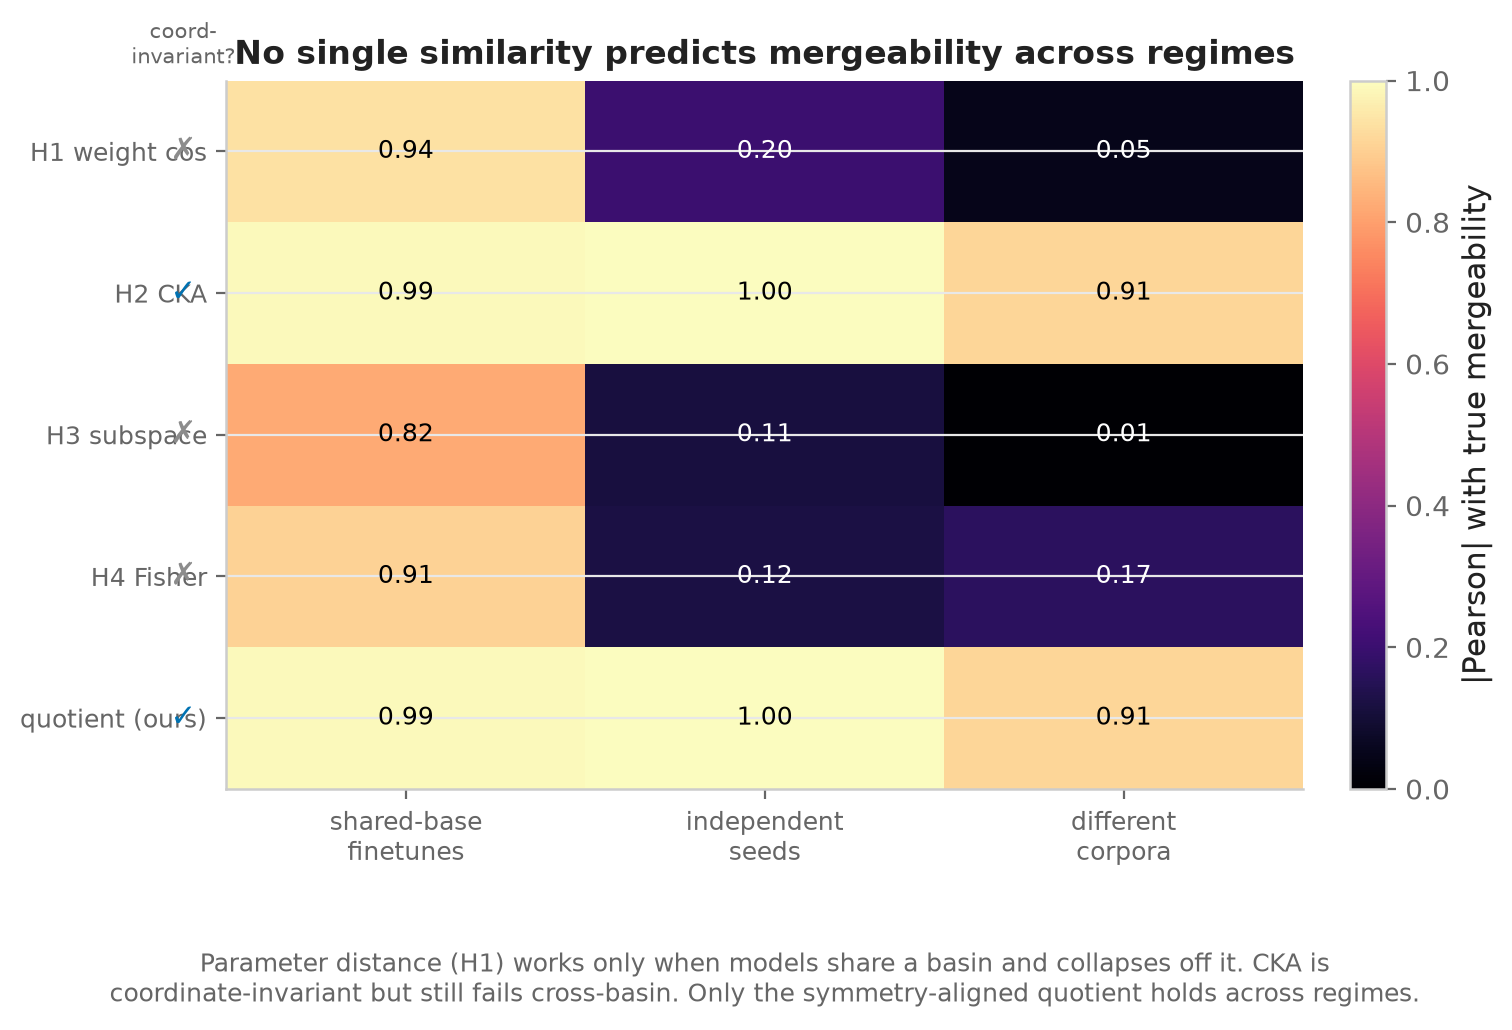
\includegraphics[width=\textwidth,height=0.74\textheight,keepaspectratio]{figures/slides_fig10_horse_race.png}
  \end{center}
  \vspace{-0.5em}\begin{center}\tiny {\tiny\texttt{\detokenize{slides_fig10_horse_race.png}}}\end{center}
\end{frame}

\begin{frame}{Slides fig11 variance partition}
  \begin{center}
    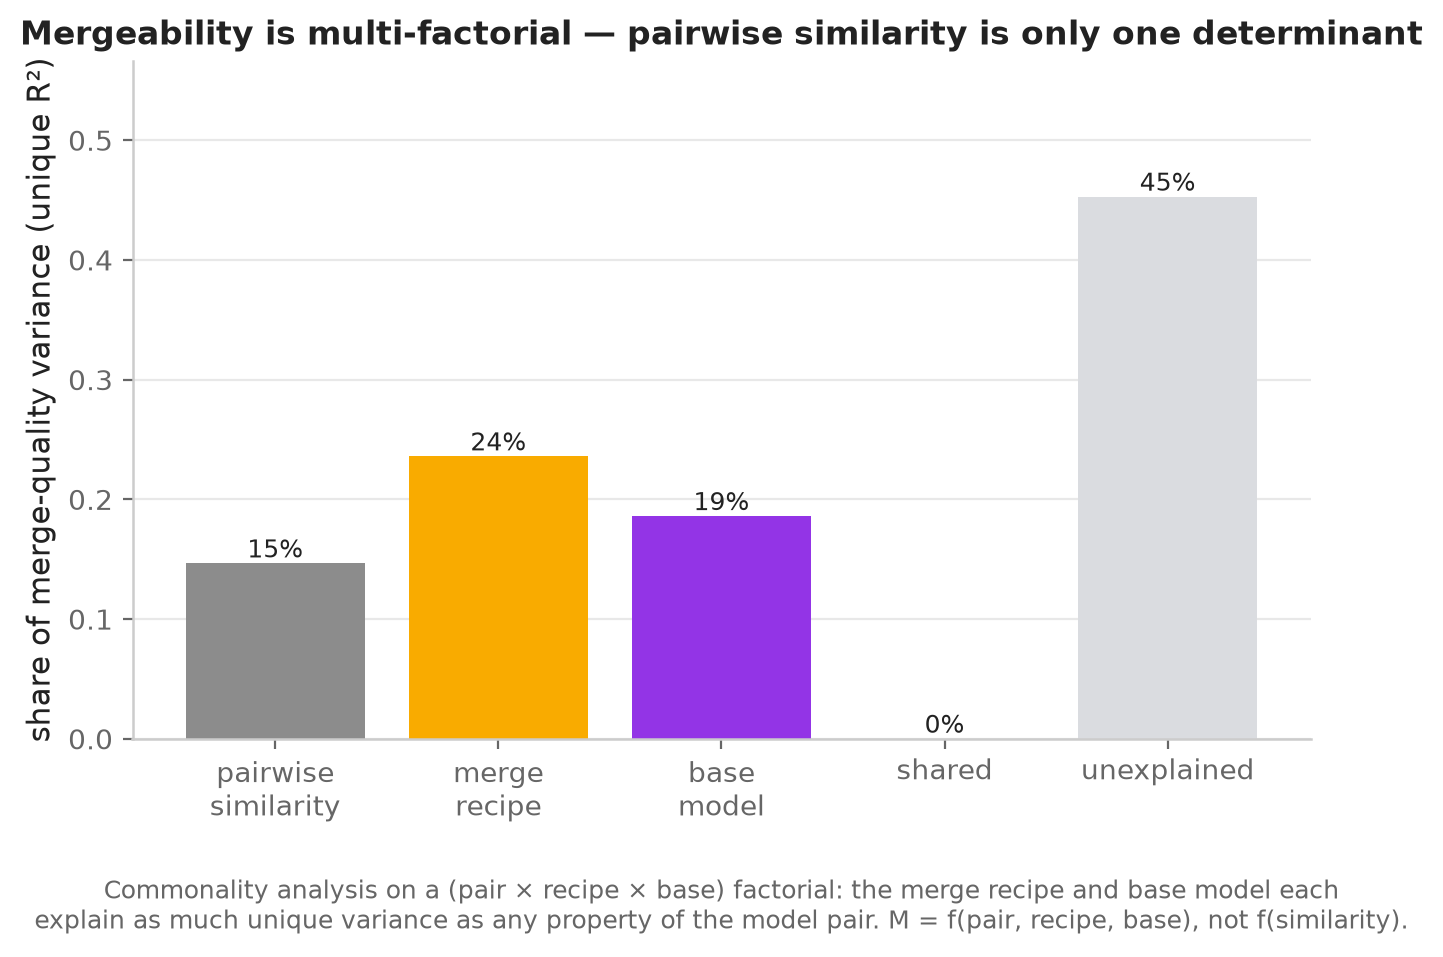
\includegraphics[width=\textwidth,height=0.74\textheight,keepaspectratio]{figures/slides_fig11_variance_partition.png}
  \end{center}
  \vspace{-0.5em}\begin{center}\tiny {\tiny\texttt{\detokenize{slides_fig11_variance_partition.png}}}\end{center}
\end{frame}

\begin{frame}{Slides fig12 goldfish regime}
  \begin{center}
    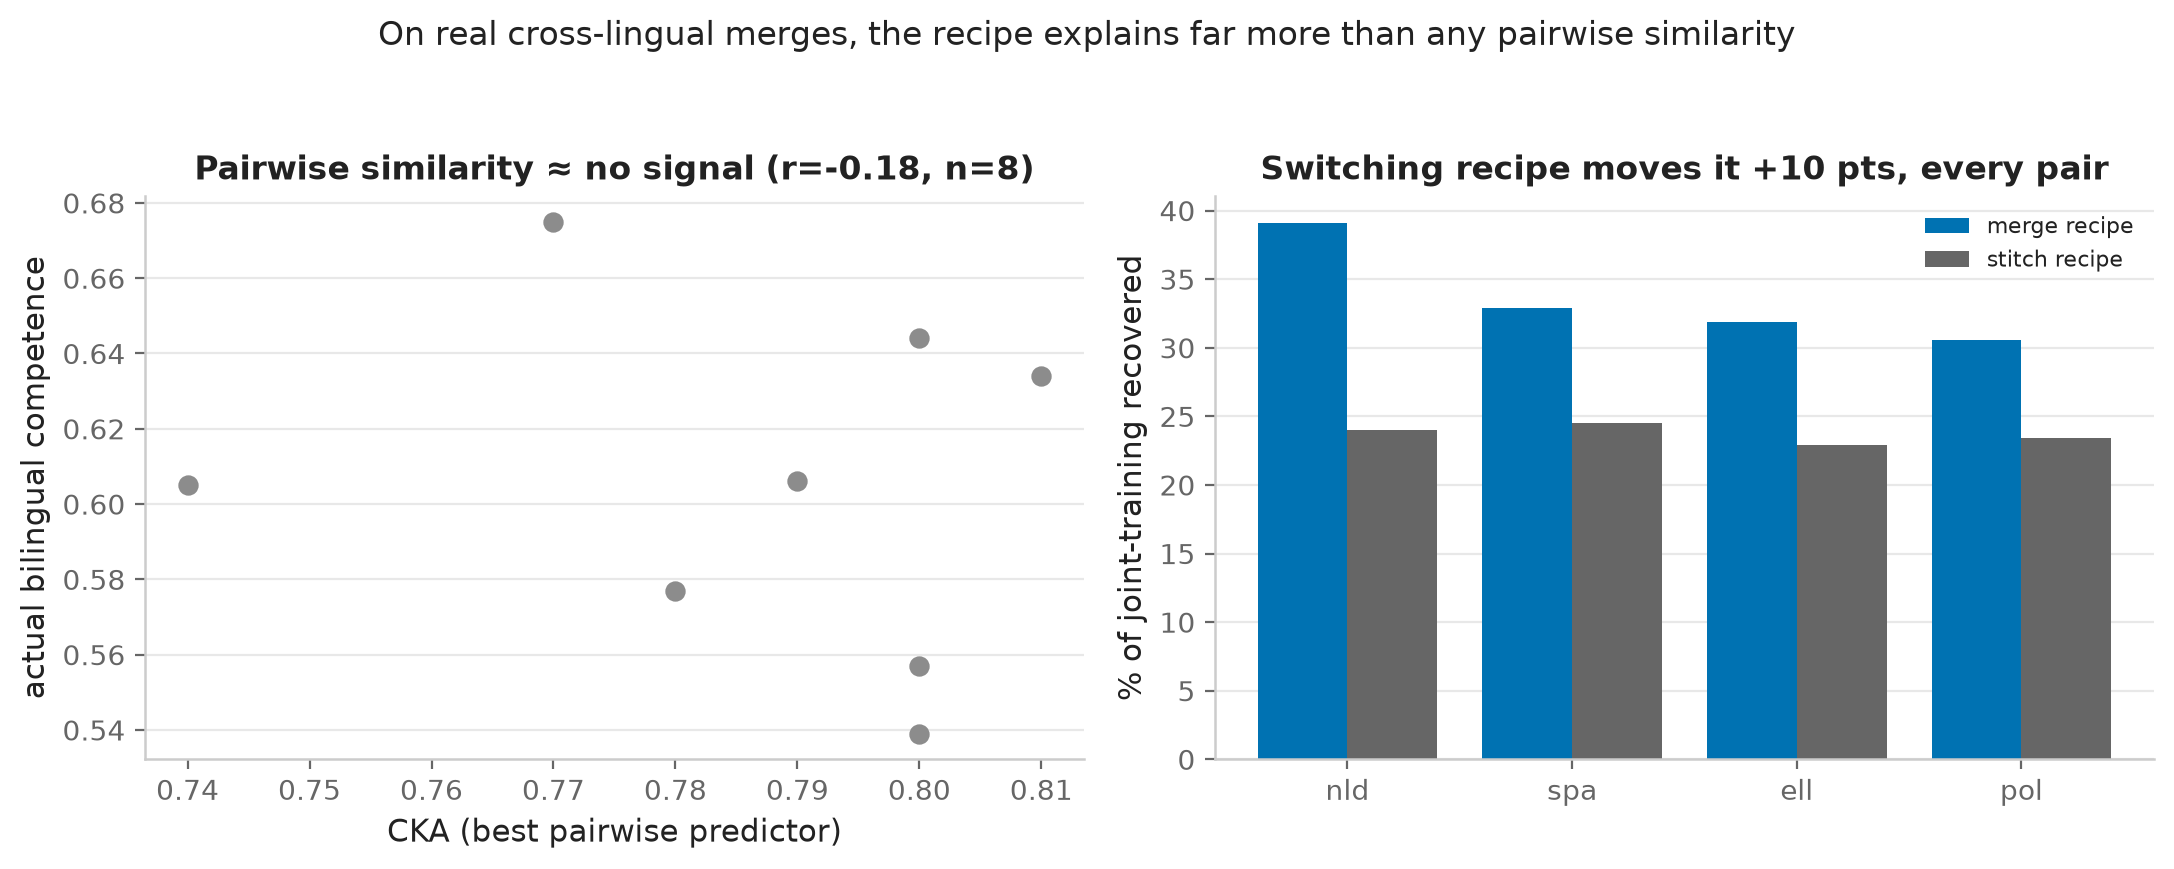
\includegraphics[width=\textwidth,height=0.74\textheight,keepaspectratio]{figures/slides_fig12_goldfish_regime.png}
  \end{center}
  \vspace{-0.5em}\begin{center}\tiny {\tiny\texttt{\detokenize{slides_fig12_goldfish_regime.png}}}\end{center}
\end{frame}

\begin{frame}{Slides fig13 mergeeval}
  \begin{center}
    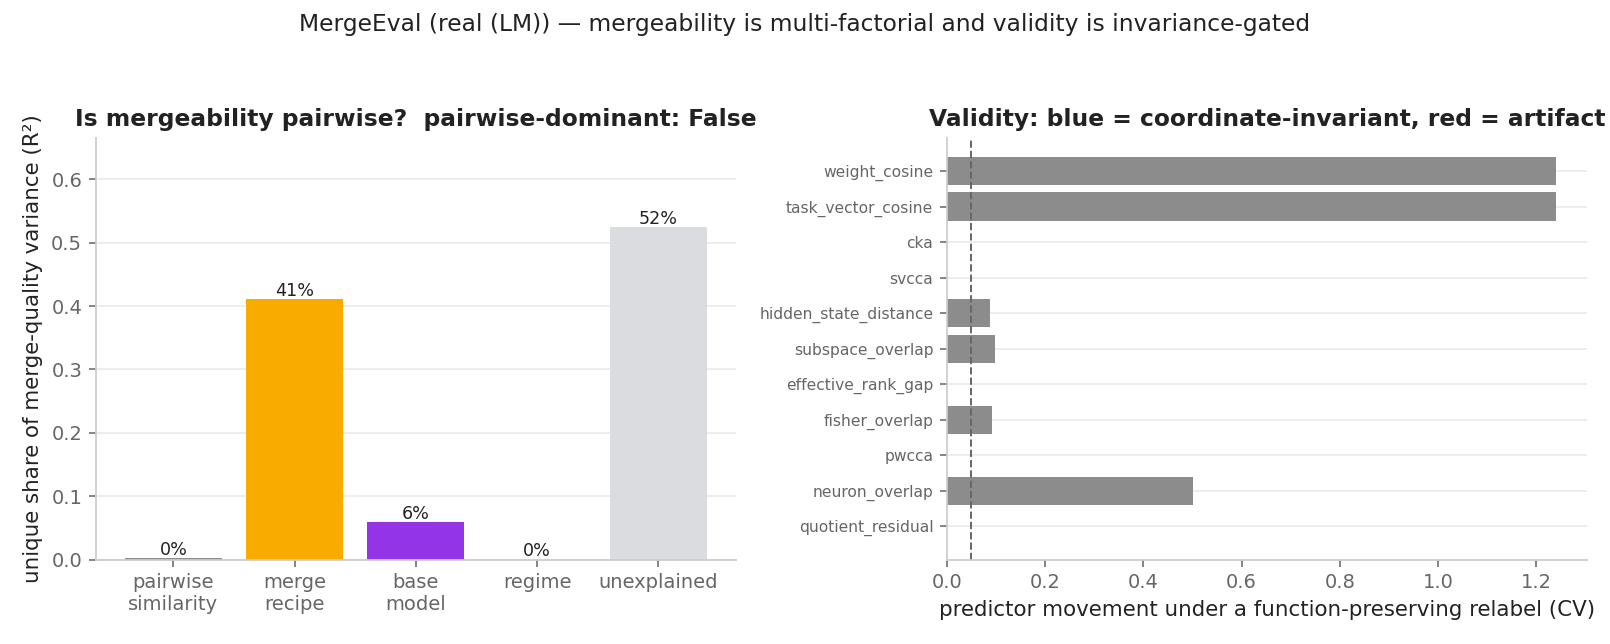
\includegraphics[width=\textwidth,height=0.74\textheight,keepaspectratio]{figures/slides_fig13_mergeeval.png}
  \end{center}
  \vspace{-0.5em}\begin{center}\tiny {\tiny\texttt{\detokenize{slides_fig13_mergeeval.png}}}\end{center}
\end{frame}

\begin{frame}{Slides fig15 mergebench}
  \begin{center}
    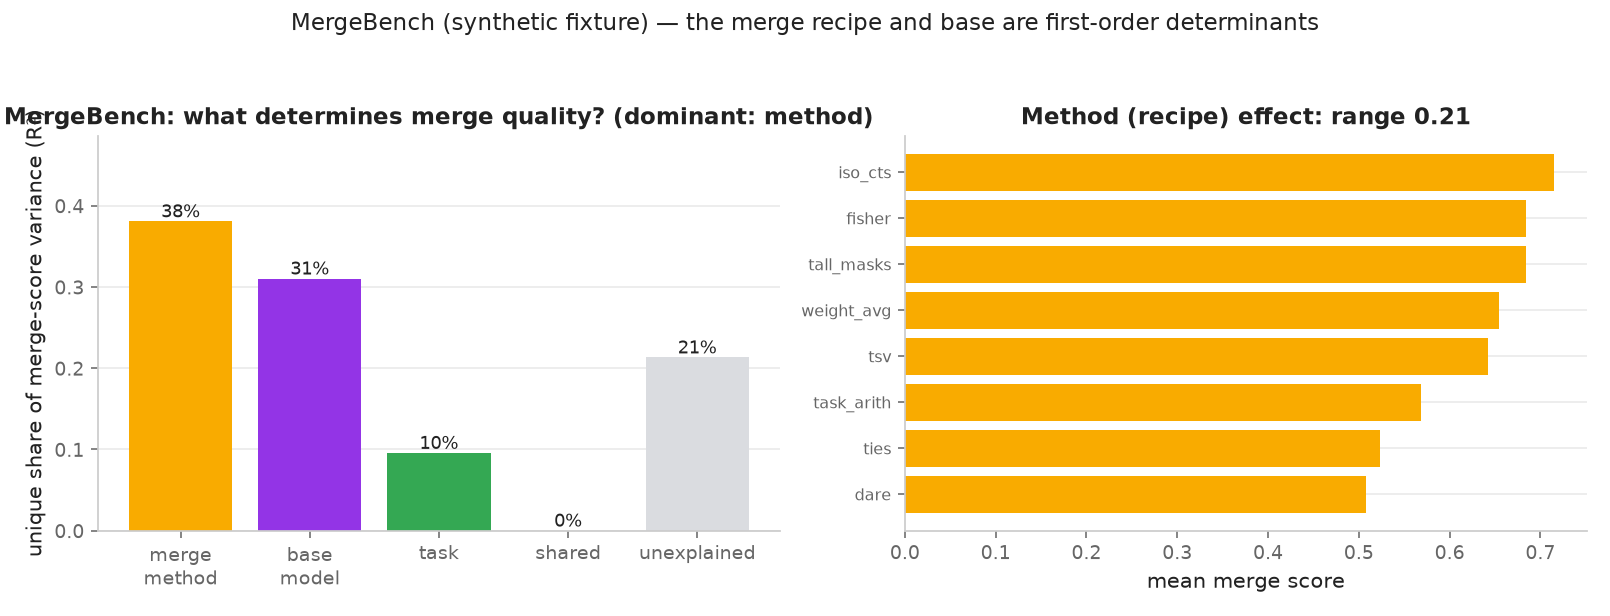
\includegraphics[width=\textwidth,height=0.74\textheight,keepaspectratio]{figures/slides_fig15_mergebench.png}
  \end{center}
  \vspace{-0.5em}\begin{center}\tiny {\tiny\texttt{\detokenize{slides_fig15_mergebench.png}}}\end{center}
\end{frame}

\begin{frame}{Slides fig16 structure}
  \begin{center}
    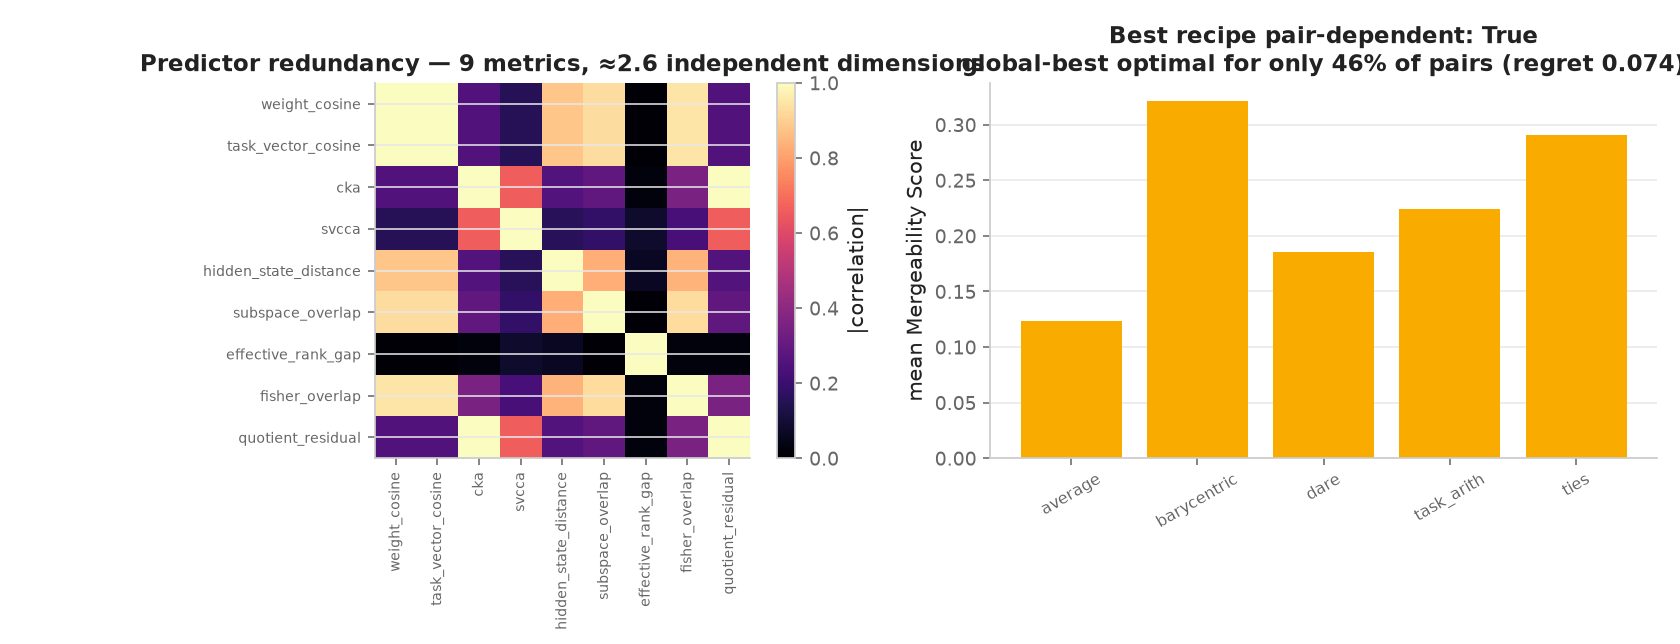
\includegraphics[width=\textwidth,height=0.74\textheight,keepaspectratio]{figures/slides_fig16_structure.png}
  \end{center}
  \vspace{-0.5em}\begin{center}\tiny {\tiny\texttt{\detokenize{slides_fig16_structure.png}}}\end{center}
\end{frame}

\begin{frame}{Slides fig17 invariance spectrum}
  \begin{center}
    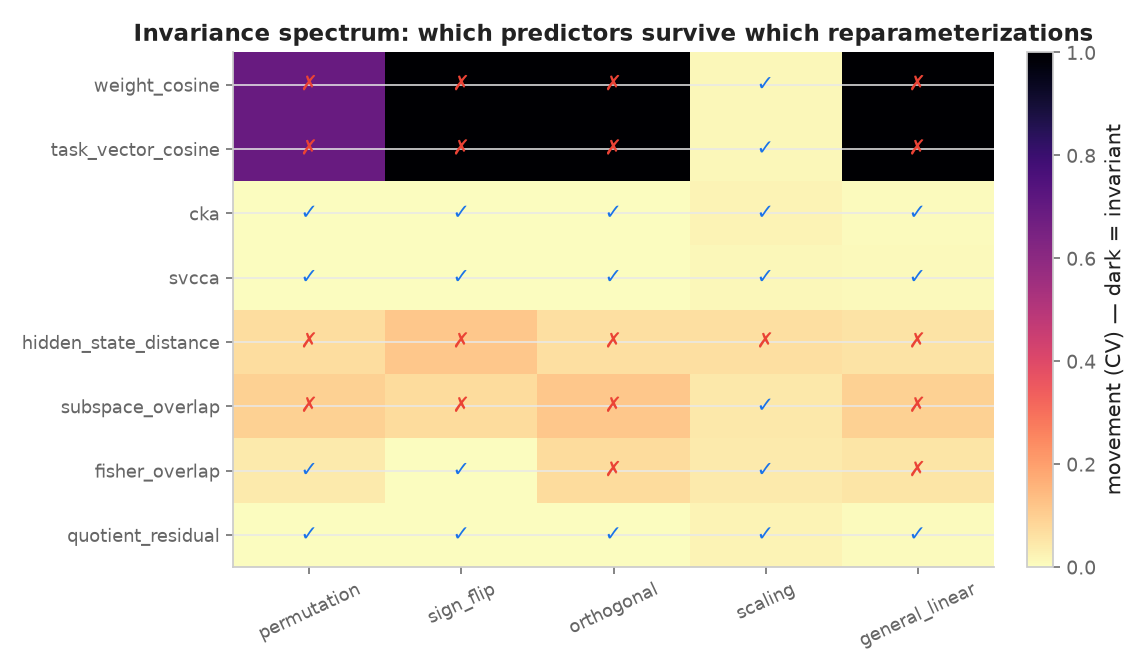
\includegraphics[width=\textwidth,height=0.74\textheight,keepaspectratio]{figures/slides_fig17_invariance_spectrum.png}
  \end{center}
  \vspace{-0.5em}\begin{center}\tiny {\tiny\texttt{\detokenize{slides_fig17_invariance_spectrum.png}}}\end{center}
\end{frame}

\begin{frame}{Slides fig18 cross study}
  \begin{center}
    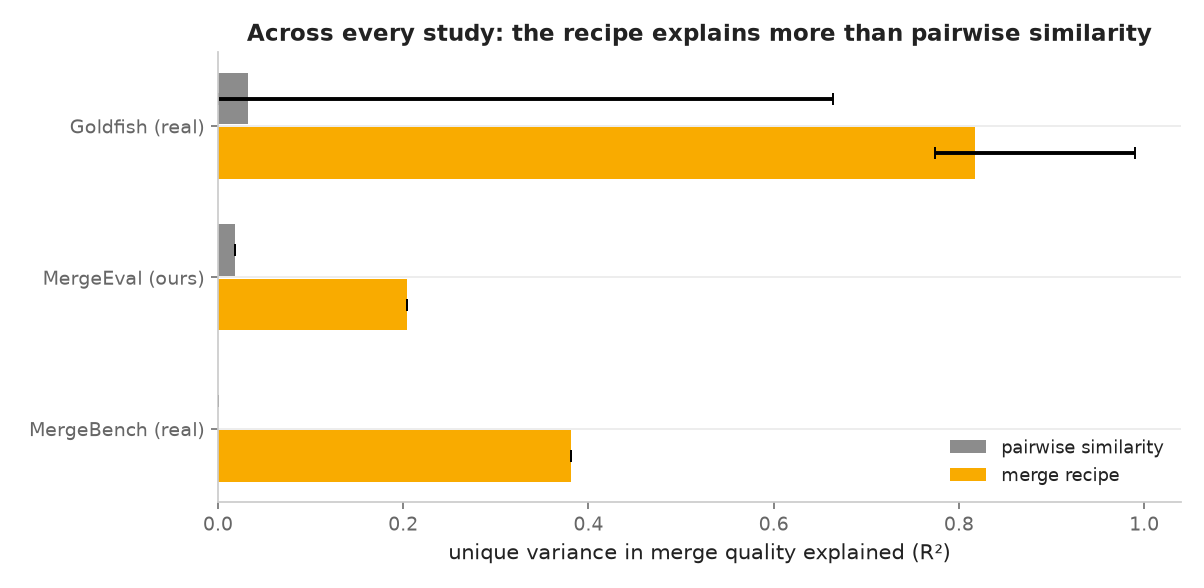
\includegraphics[width=\textwidth,height=0.74\textheight,keepaspectratio]{figures/slides_fig18_cross_study.png}
  \end{center}
  \vspace{-0.5em}\begin{center}\tiny {\tiny\texttt{\detokenize{slides_fig18_cross_study.png}}}\end{center}
\end{frame}

\begin{frame}{Slides fig19 community merges}
  \begin{center}
    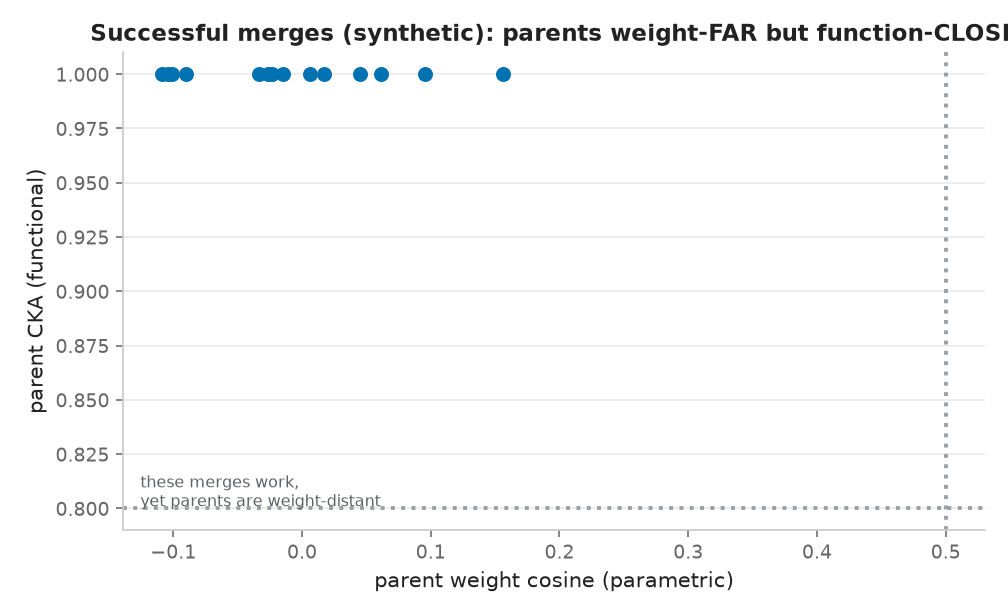
\includegraphics[width=\textwidth,height=0.74\textheight,keepaspectratio]{figures/slides_fig19_community_merges.png}
  \end{center}
  \vspace{-0.5em}\begin{center}\tiny {\tiny\texttt{\detokenize{slides_fig19_community_merges.png}}}\end{center}
\end{frame}

\begin{frame}{Slides fig6 invariance falsification}
  \begin{center}
    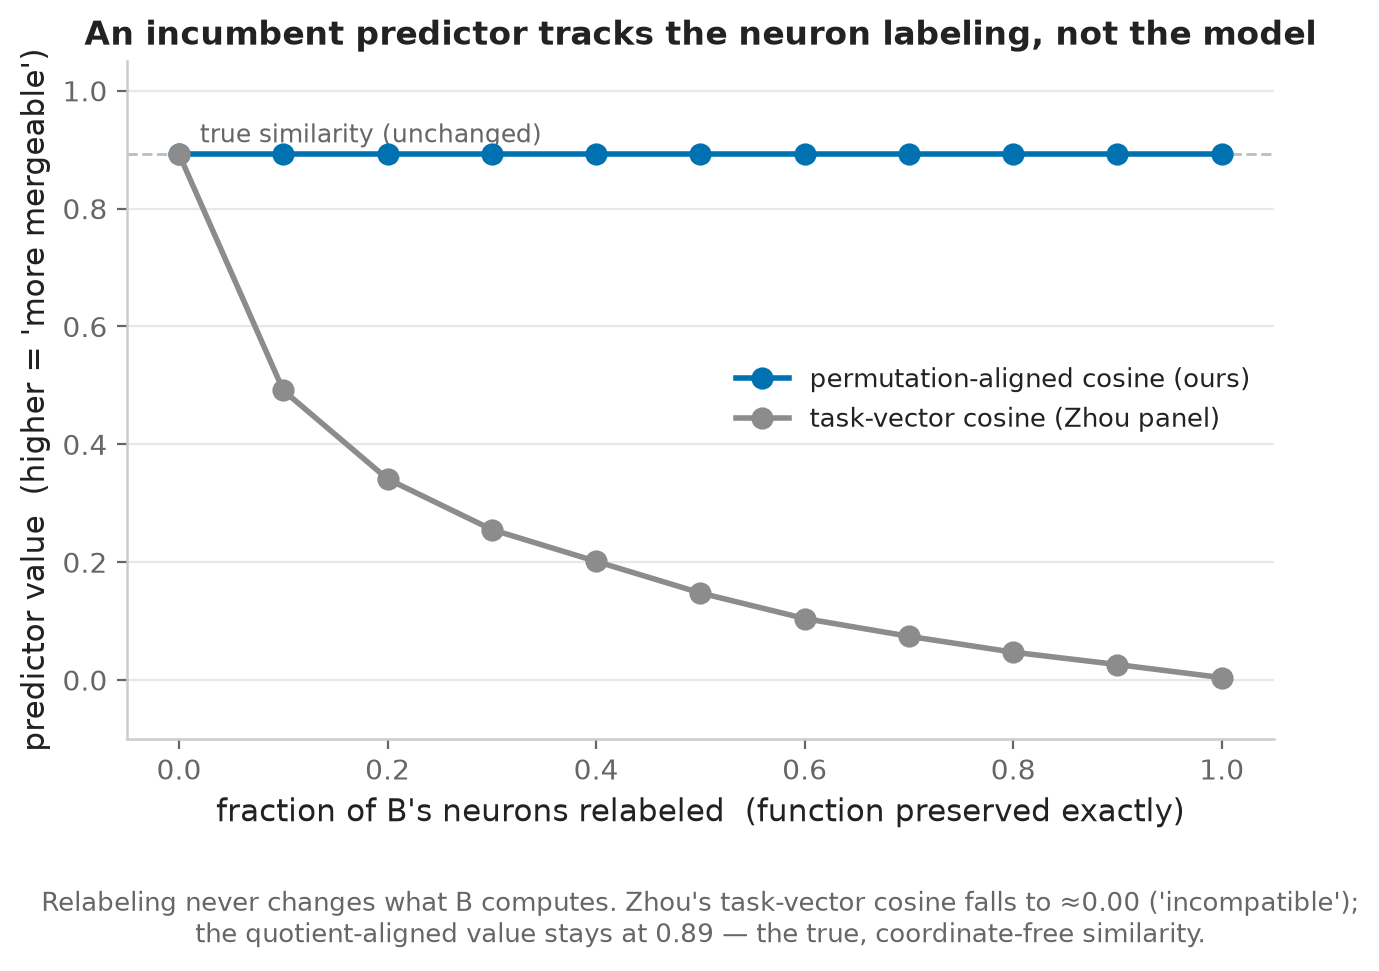
\includegraphics[width=\textwidth,height=0.74\textheight,keepaspectratio]{figures/slides_fig6_invariance_falsification.png}
  \end{center}
  \vspace{-0.5em}\begin{center}\tiny {\tiny\texttt{\detokenize{slides_fig6_invariance_falsification.png}}}\end{center}
\end{frame}

\begin{frame}{Beetle initial}
  \begin{center}
    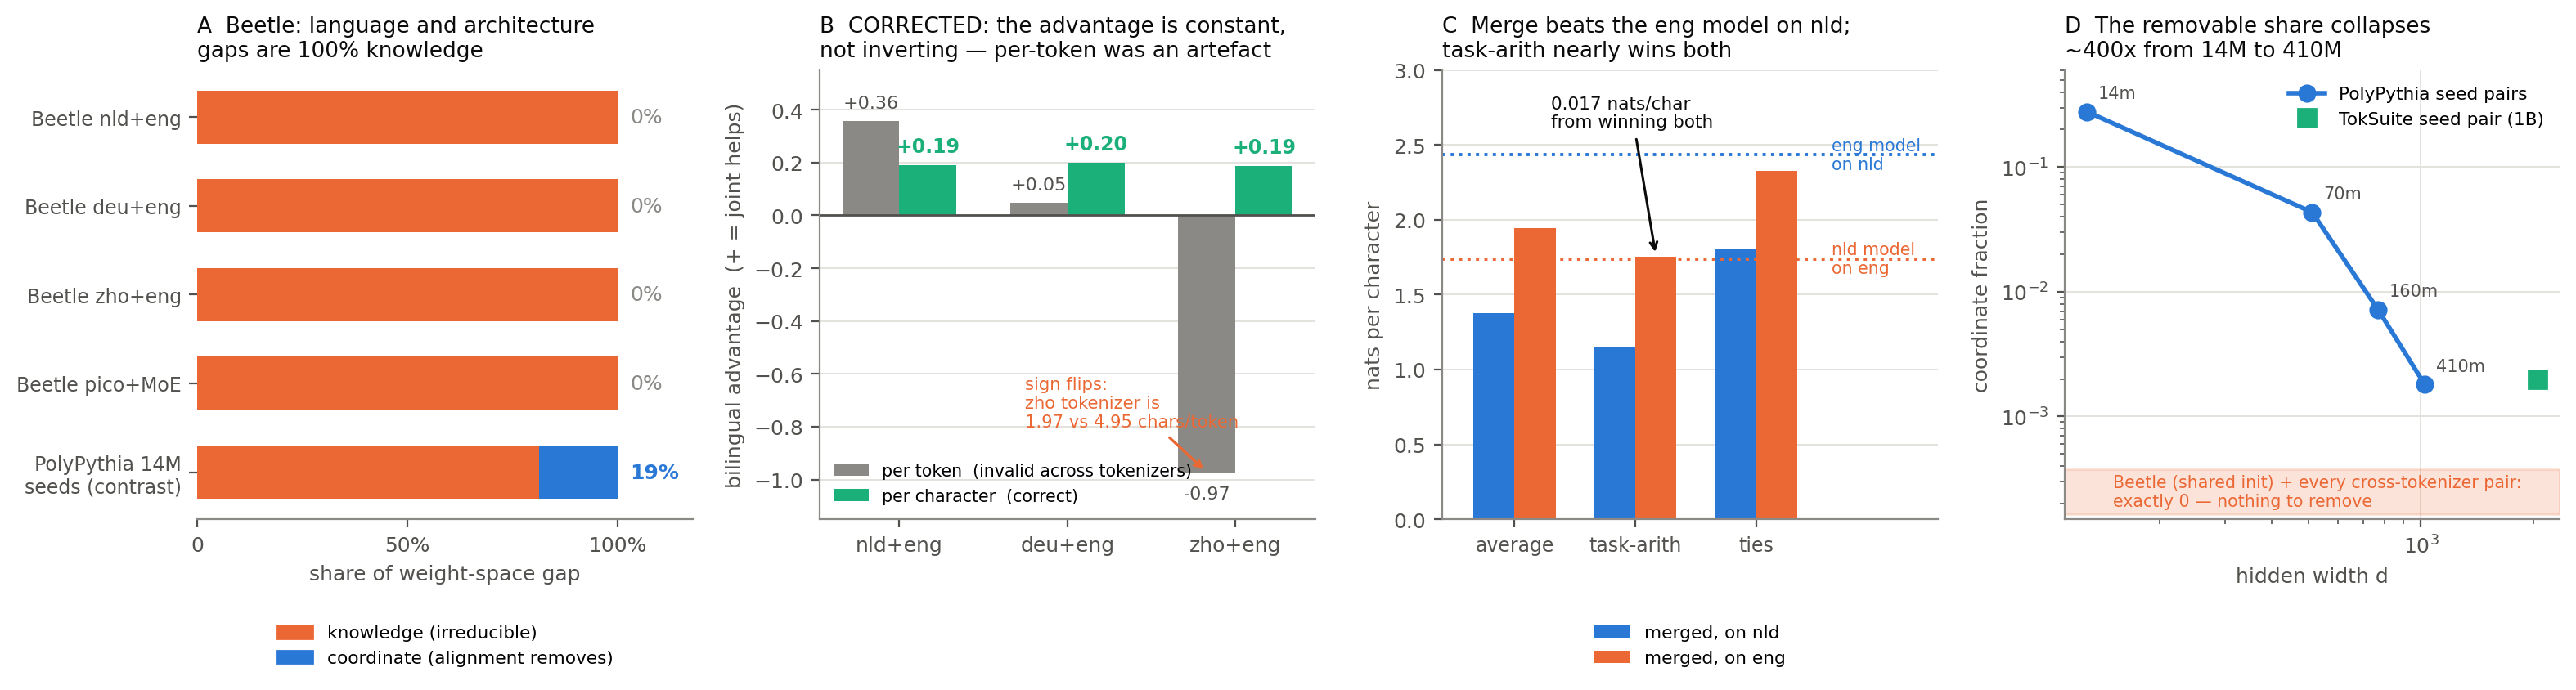
\includegraphics[width=\textwidth,height=0.74\textheight,keepaspectratio]{figures/beetle_initial.png}
  \end{center}
  \vspace{-0.5em}\begin{center}\tiny {\tiny\texttt{\detokenize{beetle_initial.png}}}\end{center}
\end{frame}

\begin{frame}{Fig rq5 schedule recovery}
  \begin{center}
    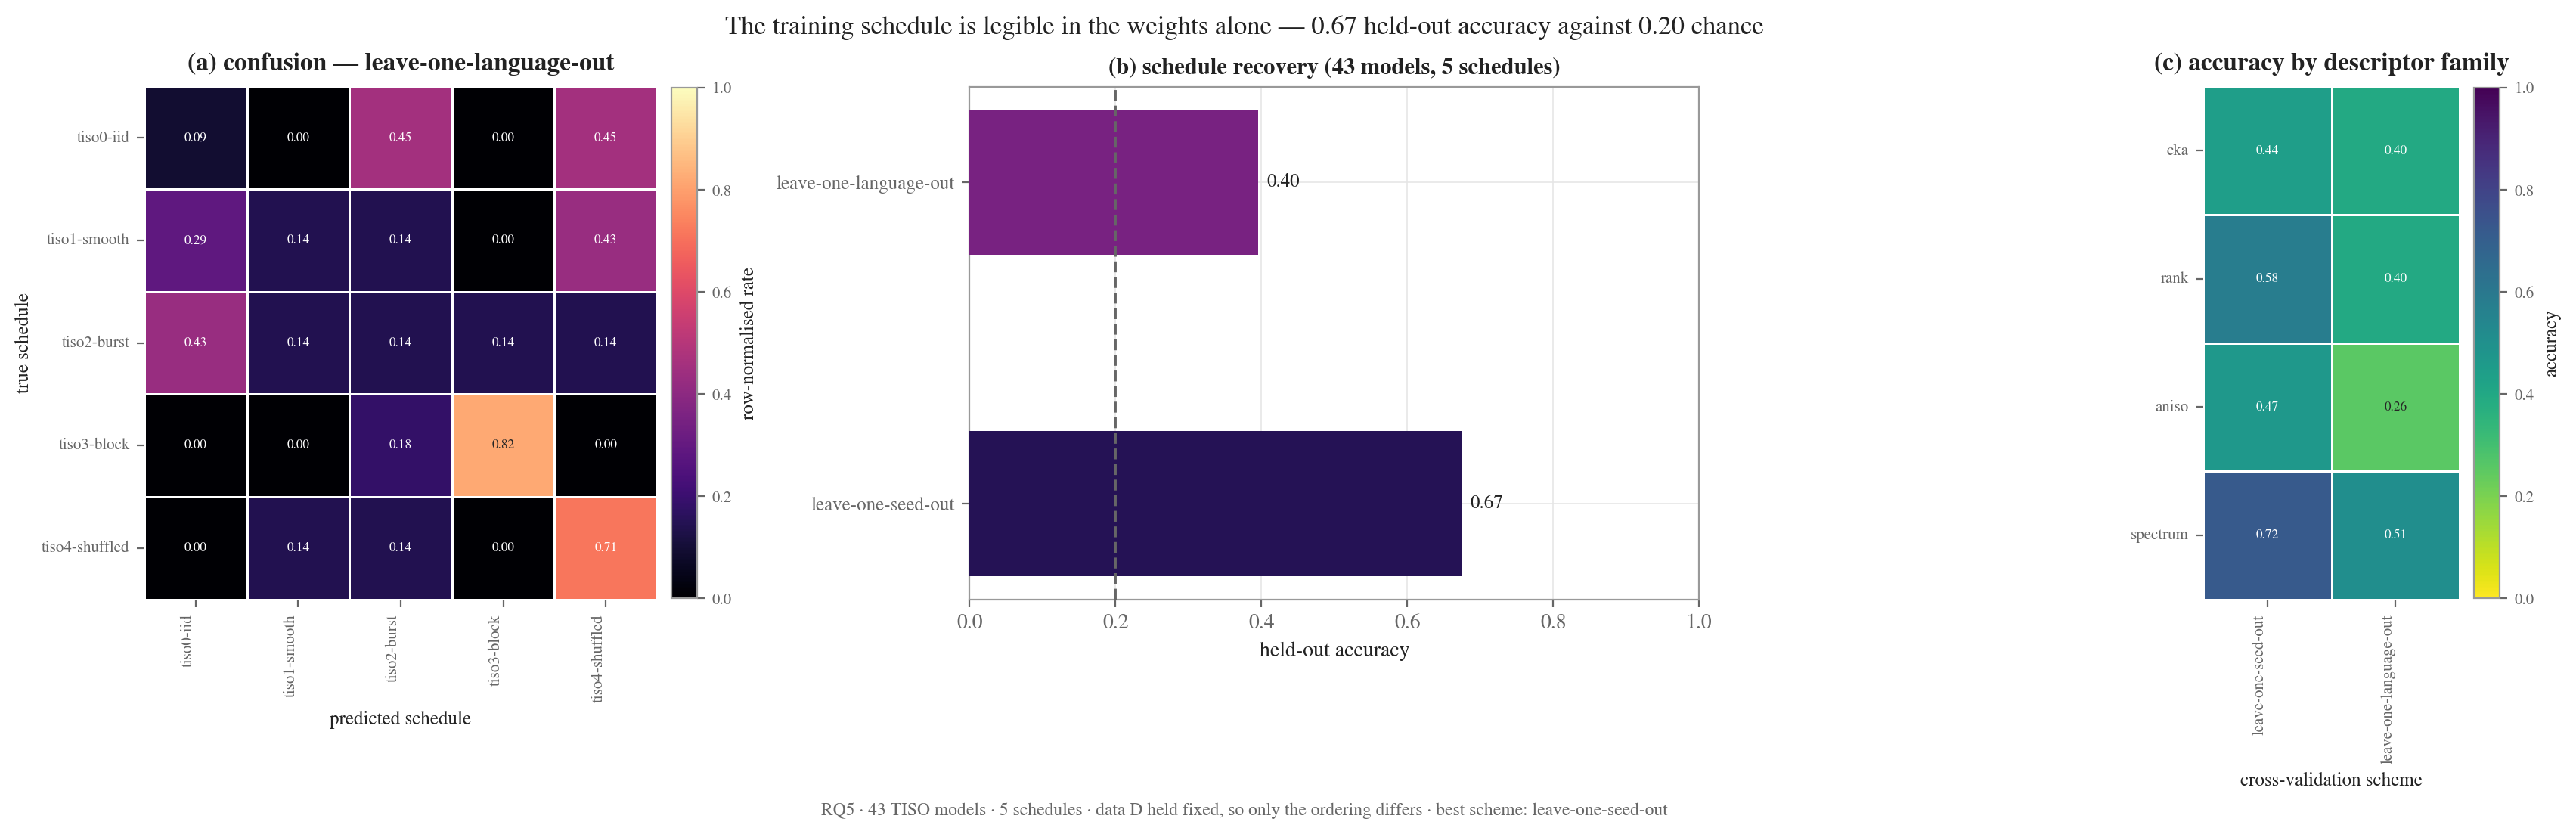
\includegraphics[width=\textwidth,height=0.74\textheight,keepaspectratio]{figures/fig_rq5_schedule_recovery.png}
  \end{center}
  \vspace{-0.5em}\begin{center}\tiny {\tiny\texttt{\detokenize{fig_rq5_schedule_recovery.png}}}\end{center}
\end{frame}

\begin{frame}{Fig rq6 merge slope curriculum}
  \begin{center}
    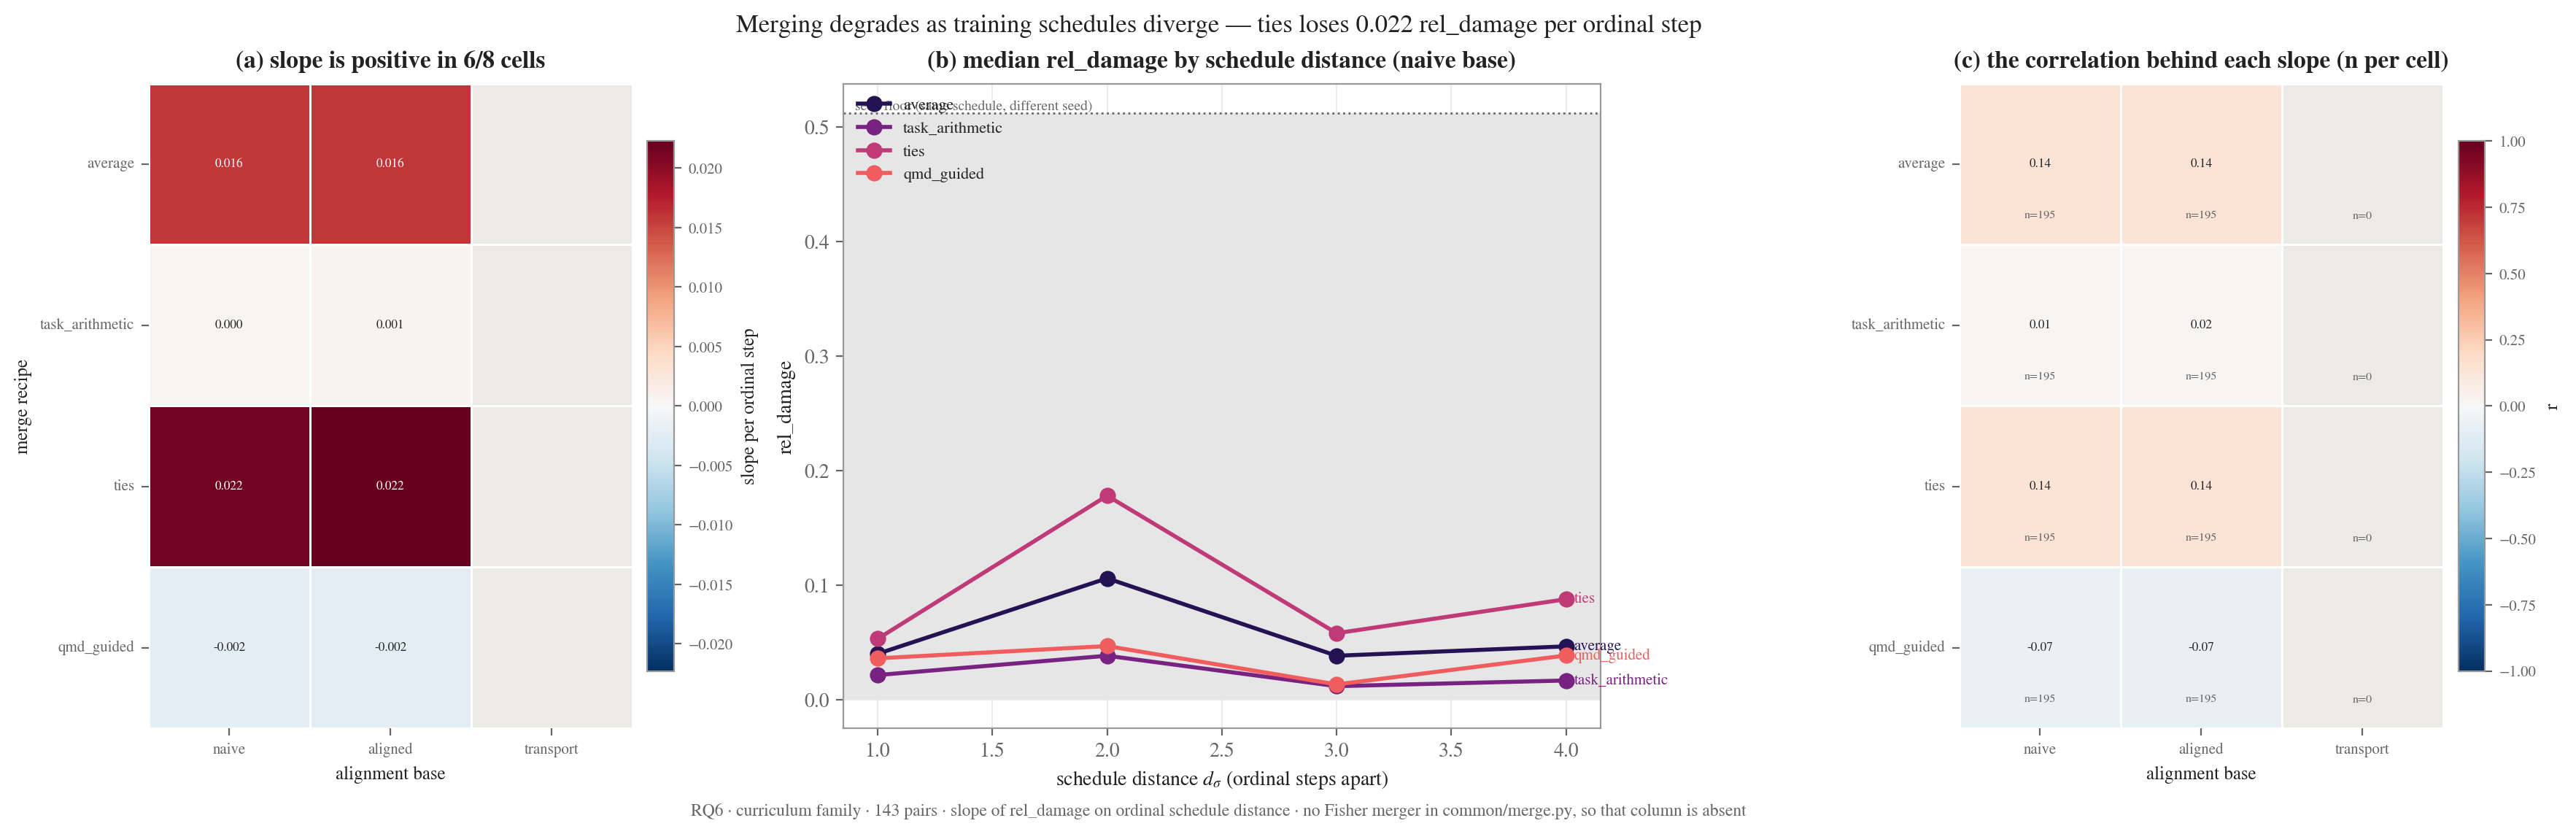
\includegraphics[width=\textwidth,height=0.74\textheight,keepaspectratio]{figures/fig_rq6_merge_slope_curriculum.png}
  \end{center}
  \vspace{-0.5em}\begin{center}\tiny {\tiny\texttt{\detokenize{fig_rq6_merge_slope_curriculum.png}}}\end{center}
\end{frame}

\begin{frame}{Fig rq7 basin separation curriculum}
  \begin{center}
    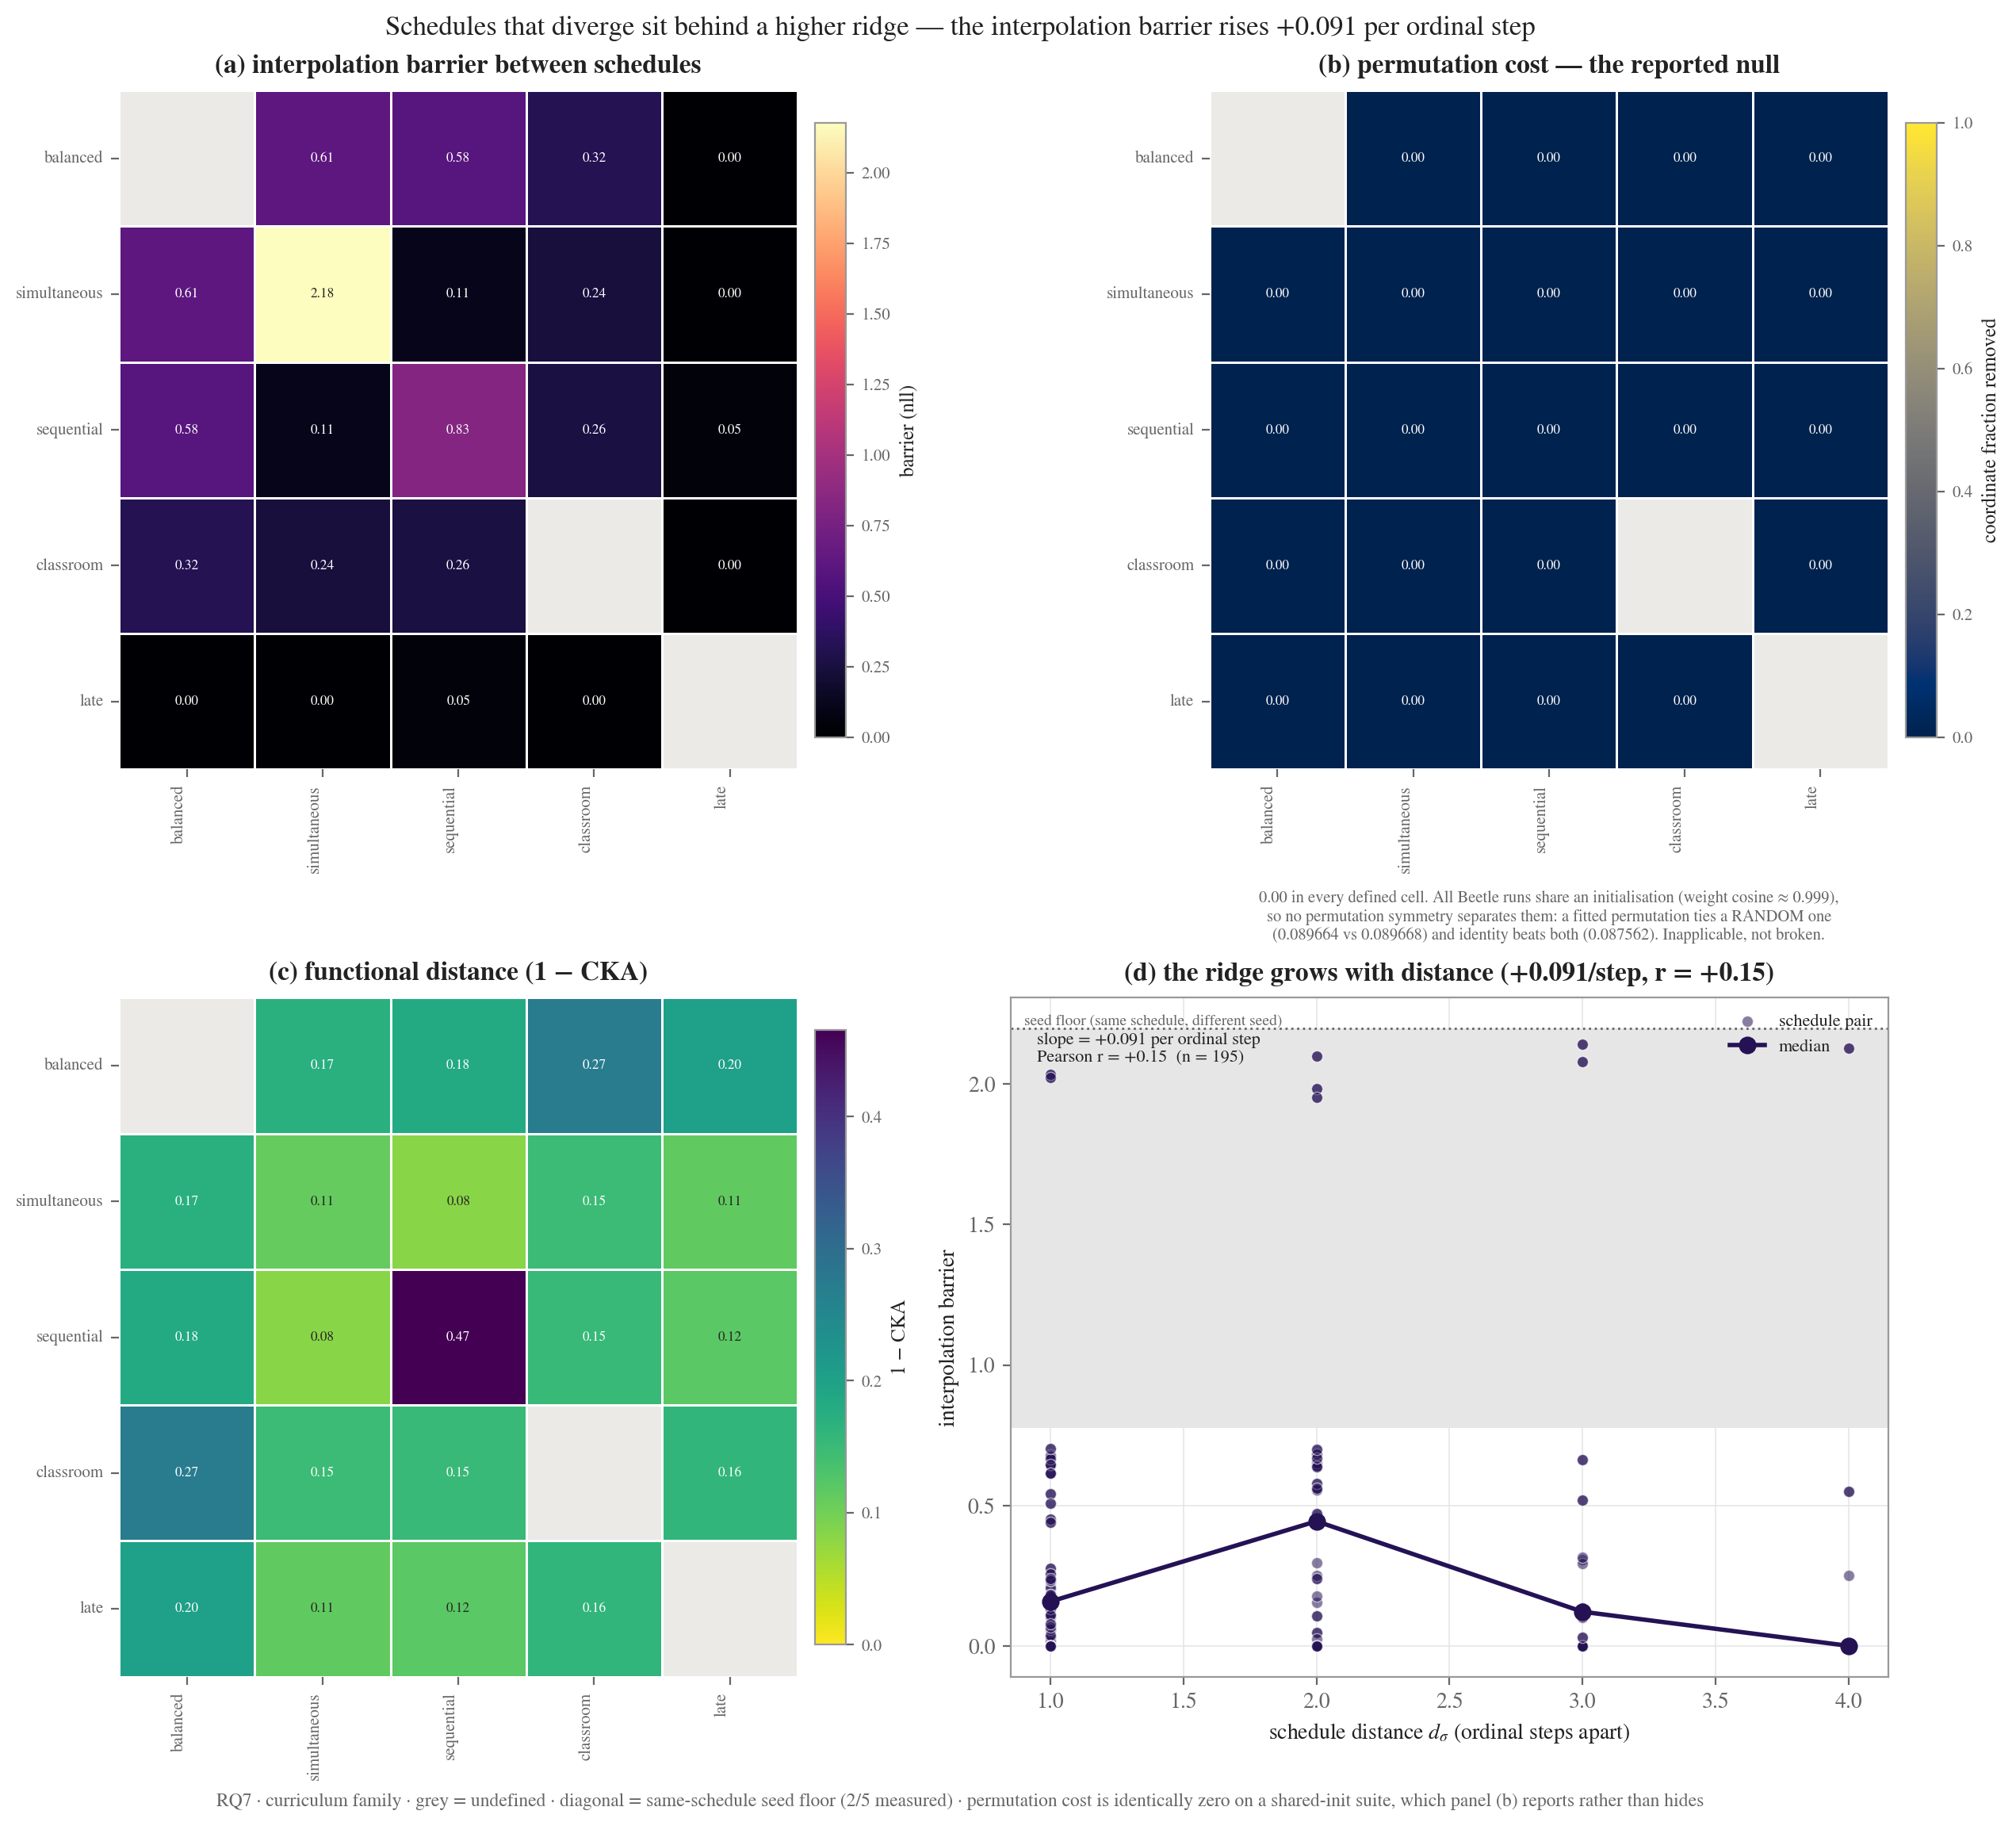
\includegraphics[width=\textwidth,height=0.74\textheight,keepaspectratio]{figures/fig_rq7_basin_separation_curriculum.png}
  \end{center}
  \vspace{-0.5em}\begin{center}\tiny {\tiny\texttt{\detokenize{fig_rq7_basin_separation_curriculum.png}}}\end{center}
\end{frame}

\begin{frame}{Fig rq8 developmental}
  \begin{center}
    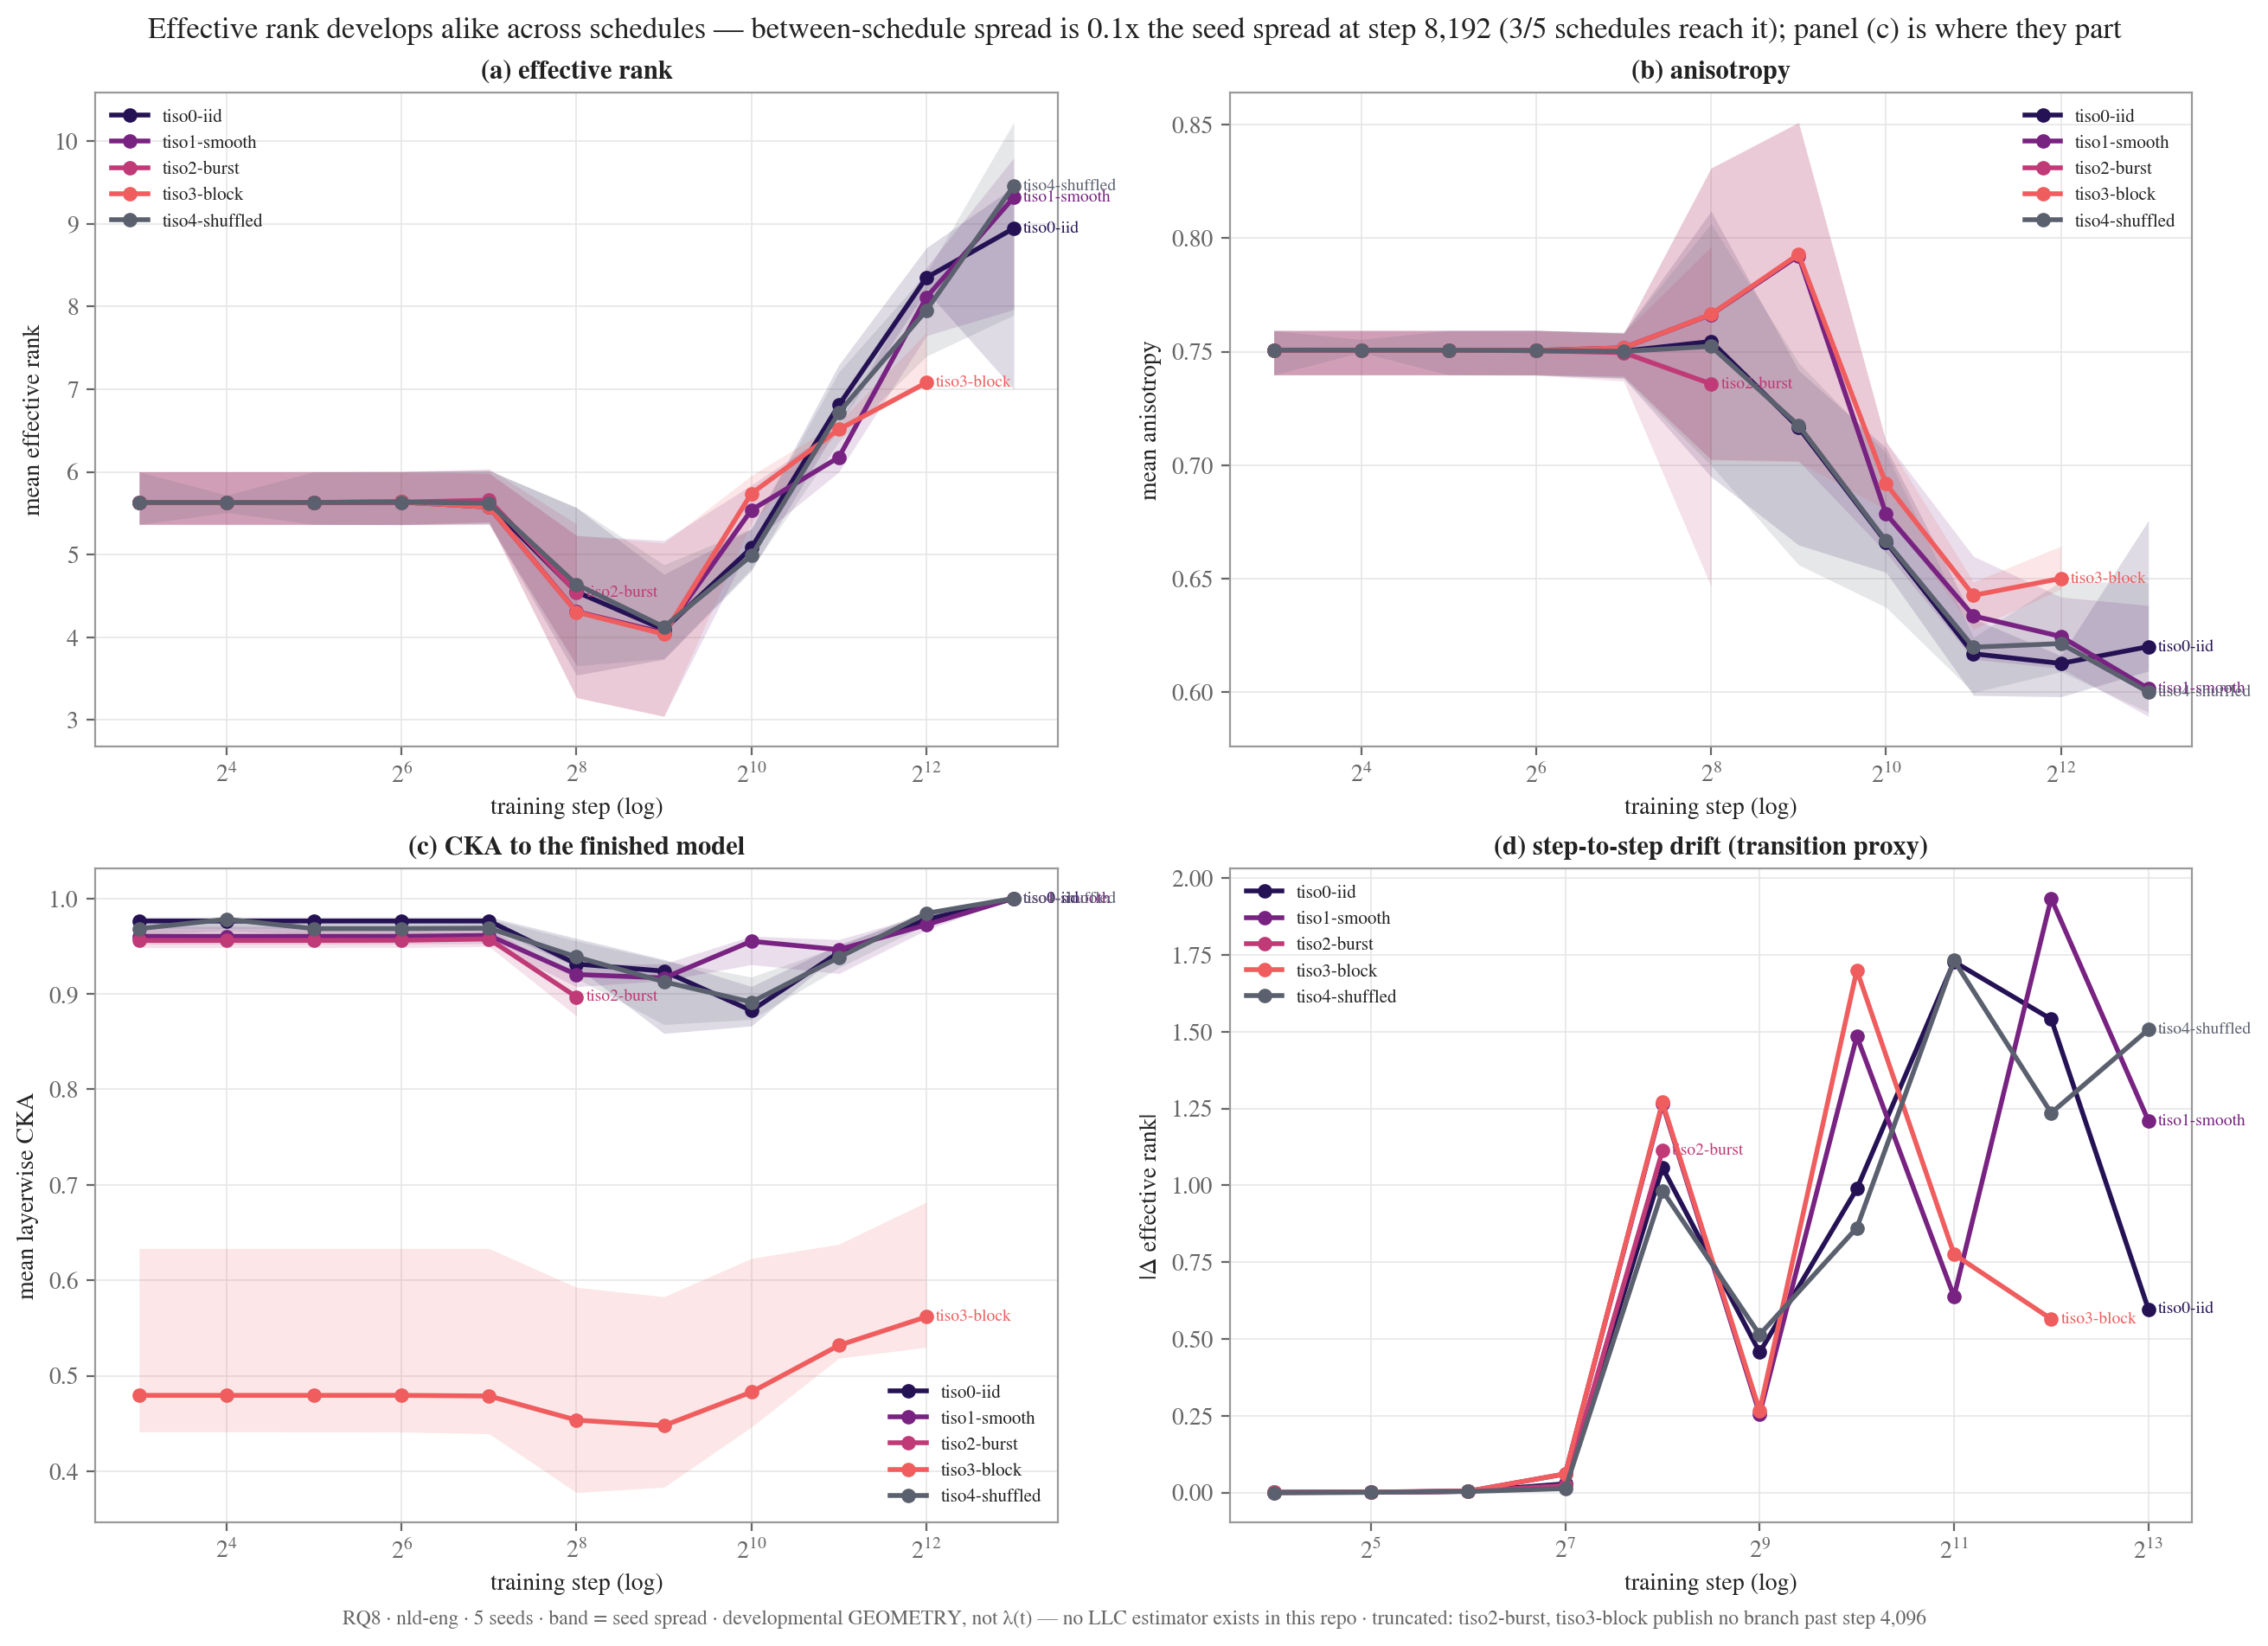
\includegraphics[width=\textwidth,height=0.74\textheight,keepaspectratio]{figures/fig_rq8_developmental.png}
  \end{center}
  \vspace{-0.5em}\begin{center}\tiny {\tiny\texttt{\detokenize{fig_rq8_developmental.png}}}\end{center}
\end{frame}

\begin{frame}{Zoo heatmaps}
  \begin{center}
    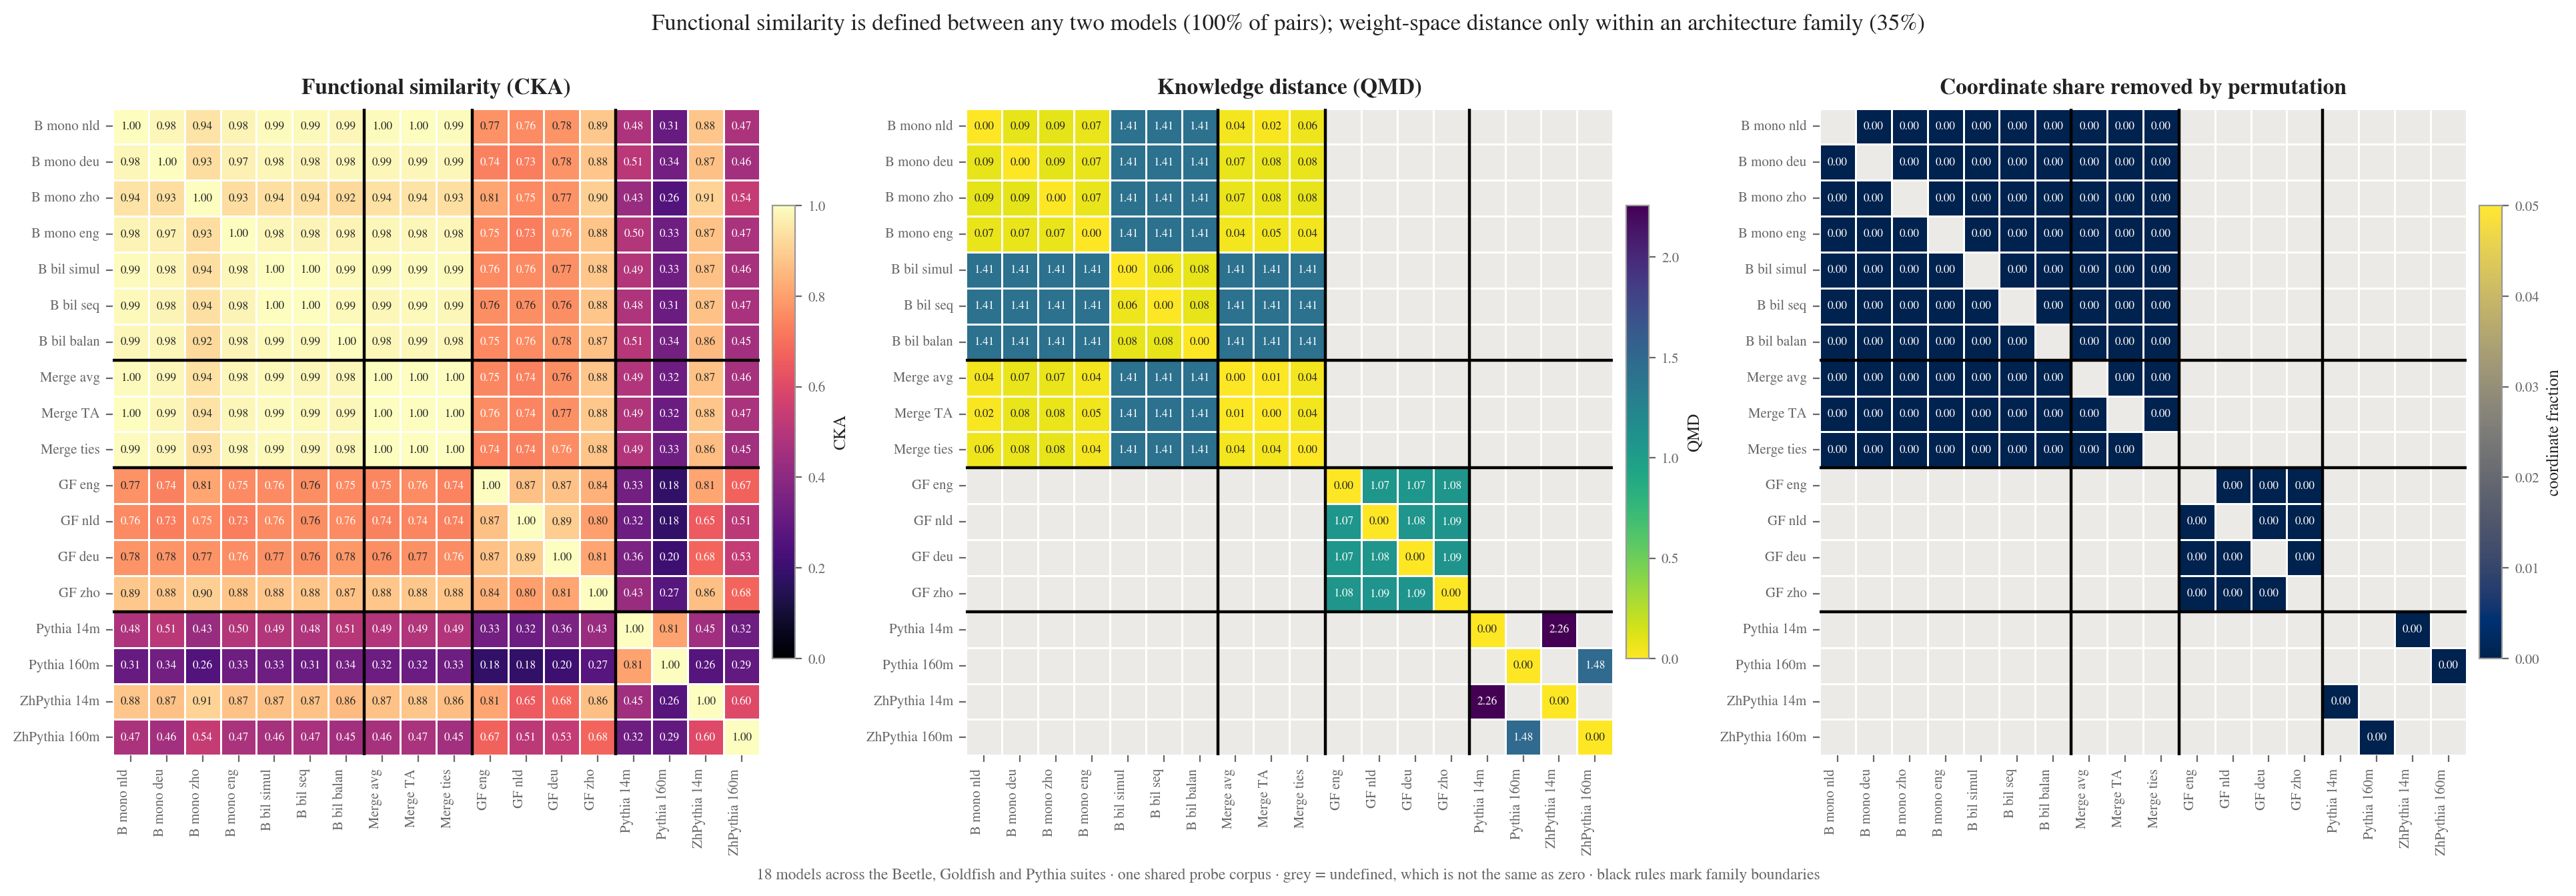
\includegraphics[width=\textwidth,height=0.74\textheight,keepaspectratio]{figures/zoo_heatmaps.png}
  \end{center}
  \vspace{-0.5em}\begin{center}\tiny {\tiny\texttt{\detokenize{zoo_heatmaps.png}}}\end{center}
\end{frame}

\begin{frame}
  \centering\Large Thank you
\end{frame}

\end{document}
